%%%%%%%%%%%%%%%%%%%%%%%%%%%%%%%%%%%%%%%%%%%%%%%%%%%%%%%
% A template for Wiley article submissions.
% Developed by Overleaf. 
%
% Please note that whilst this template provides a 
% preview of the typeset manuscript for submission, it 
% will not necessarily be the final publication layout.
%
% Usage notes:
% The "blind" option will make anonymous all author, affiliation, correspondence and funding information.
% Use "num-refs" option for numerical citation and references style.
% Use "alpha-refs" option for author-year citation and references style.

%\documentclass[blind, num-refs]{wiley-article}
\documentclass[alpha-refs]{wiley-article}

% Add additional packages here if required
\usepackage{siunitx}
\usepackage{natbib} % added for reference management 
\usepackage{flafter} % no backward float to get figure numbers is right order 
\usepackage{subcaption} % added for subfigures 
\usepackage[section]{placeins} % impedes floating to next section (use only for outline!) 
\usepackage{lineno} % line numbers 
\usepackage[left=3cm,top=3cm,right=3cm,bottom=3cm,bindingoffset=0.5cm]{geometry}
\usepackage{wrapfig}  % added package 


% Update article type if known
\papertype{International Journal of Climatology}
% Include section in journal if known, otherwise delete
\paperfield{Journal Section}

\title{Temporal and spatial variations of convection and precipitation over the Tibetan Plateau based on recent satellite observations. Part I: Cloud climatology derived from \textit{CloudSat} and \textit{CALIPSO}}

% List abbreviations here, if any. Please note that it is preferred that abbreviations be defined at the first instance they appear in the text, rather than creating an abbreviations list.
\abbrevs{TP, Tibetan Plateau; CFAD, contoured-frequency-by-altitude-diagram; CPR, cloud profiling radar; CCN, cloud condensation nuclei; IN, ice condensation nuclei}



% Include full author names and degrees, when required by the journal.
% Use the \authfn to add symbols for additional footnotes and present addresses, if any. Usually start with 1 for notes about author contributions; then continuing with 2 etc if any author has a different present address.
\author[1\authfn{1}]{Julia Kukulies}
\author[1\authfn{1}]{Deliang Chen}
\author[2\authfn{1}]{Minghuai Wang}

%\contrib[\authfn{1}]{Equally contributing authors.}

% Include full affiliation details for all authors
\affil[1]{Regional Climate Group, Department of Earth Sciences, University of Gothenburg, Gothenburg, Sweden}
\affil[2]{School of Atmospheric Sciences, Nanjing University, Jiangsu, Nanjing, China}

\corraddress{Deliang Chen, Department of Earth Sciences, University of Gothenburg, Box 460, 405 30 Gothenburg, Sweden.}
\corremail{deliang@gvc.gu.se}


\fundinginfo{The Strategic Priority Research Program of Chinese Academy of Sciences (XDA2006040103), 2. The Swedish Research Council (2014-5320 and 2017-03780), 3. The Swedish Foundation for International Cooperation in Research and Higher Education (CH2015-6226), 4) The National Natural Science Foundation of China (91537210).}

% Include the name of the author that should appear in the running header
\runningauthor{Kukulies et al.}

\begin{document}
\openup 1em % double line spacing

\maketitle

\begin{abstract}

This sequence of papers, consisting of two parts, examines temporal and spatial variations of convection and precipitation over the Tibetan Plateau (TP) based on recent satellite observations. Here in Part 1 seasonal and diurnal variations of cloud vertical structure and cloud properties have been derived from four combined \textit{CloudSat} and \textit{CALIPSO} satellite datasets and compared between three subregions in the TP which are marked by different large-scale atmospheric circulations and moisture sources. The results show that the plateau is generally dominated by low-level single-layer clouds and stratiform cloud types. Cloud occurrence frequencies peak during the summer monsoon season between May and September and are generally higher during daytime compared to nighttime in all the three subregions. The fraction of detected ice cloud layers in the TP domain exceeds 50 \% during all months and 80 \% between January and April. While ice cloud layers occur as altostratus clouds in the westerly-dominated north and transition zone, high level cirrus cloud occur frequently accompanied by lower level cumulus clouds in the monsoon-dominated south, especially during nighttime. This study complements previous satellite observations of clouds over the TP and reveals firstly the high contribution of stratiform ice cloud layers in the westerly-dominated north, secondly the importance of the monsoon season which outweighs day-night differences and affects the examined cloud parameters in all regions and finally the significant regional differences of cloud characteristics within the plateau. It is therefore suggested to focus on the relative importance of stratification, mesoscale convective systems and advection in future studies on hydro-climatic changes in the TP region.

% Please include a maximum of seven keywords! 
\keywords{Tibetan Plateau, \emph{CloudSat}, climatology, Indian summer monsoon, westerlies, cloud vertical structure, ice clouds}
\end{abstract}

\section{Introduction}
\linenumbers


The Tibetan Plateau (TP) is also referred to as the Third Pole, because it stores the largest amounts of fresh water after the Arctic and Antarctica \citep{yao2012TPE,yao2018recent}. With an average elevation above 4000 m a.s.l. over an area of 5 million km$^2$ \citep{yao2012TPE}, it is the most extensive high altitude region of the world. It represents also one of the most sensitive regions to climate change, because intensive surface heating which is reinforced by different feedback mechanisms have led to enhanced atmospheric warming, glacier retreat and an accelerated hydrological cycle \citep{bibi2018climatic}. 

\citet{EDW2015} describe the TP as an outstanding example for elevation-dependent warming (EDW) and \citet{EDW_tp2009} suggest that cloud-radiation interactions are one of the underlying mechanisms that contribute to this observed effect of accelerated warming at higher elevations over the TP. Station observations and model simulations suggest that decreasing cloud occurrences during daytime have reduced the cloud albedo of the region and this in combination with increasing low-level clouds during nighttime led to an increase of minimum temperatures \citep{duan2006changeclds}. However, because the effect of clouds on the regional climate and its linkages to precipitation are dependent on different cloud macro- and microphysical properties \citep{IPCC_cloudsaerosols}, it is crucial to understand the temporal and spatial variations of these in addition to the total cloud amount \citep{cl15_2}. Spaceborne active remote sensing provides a useful tool for climatological studies of various cloud parameters at a high spatio-temporal resolution (including the vertical dimension) \citep{stephens2002cloudsat}, especially in regions like the TP where meteorological stations are sparsely distributed.


Several previous studies have used active remote sensing techniques, in order to examine convection over the TP \citep{cu13, cu16, cu16_2, cu17,cu17_2, cu17_4, himawari2018diurnal}. \citet{cu16} have found that cumulus clouds from shallow convection are among the most common cloud types over the TP, especially between June and August, when the summer monsoon dominates the moisture transport to the region. Climate model simulations suggest that these cumulus clouds hamper the development of stratiform cloud layers over large areas \citep{cu17_6}. Whereas deep convection cells seem to dominate the southeastern parts of the plateau \citep{cu08, shallowconvection2011intercomparison, m11_2} and contribute to the transport of moisture and precipitation over the southern mountain ranges \citep{cu16_5}, convection is generally shallow compared to the surrounding regions \citep{shallowconvection2011intercomparison}. \citet{cu17_4} describe a \textit{compression effect}, referring to the low vertical extents of observed cloud layers over the TP. Since these result from both relatively low cloud base and top heights above ground level, clouds have a net cooling effect in the region \citep{cu17_4}. However, while the above named studies have mainly focused on the summer monsoon season, there is insufficient knowledge about the seasonality and diurnal variations of cloud types other than cumulus. The occurrence of ice clouds have, for example, only been addressed in a few studies based on first-generation passive satellites \citep{cirrus2005MODIS} or measurements from single stations \citep{cirrus2013naqu}. Moreover, regional differences of cloud occurrences and properties within the TP as well as the linkages between convection and precipitation remain unexplored to a large extent. For these reasons, recent satellite observations from \textit{CloudSat} and \textit{CALIPSO} were used in this study to examine seasonal and diurnal variations of cloud characteristics in three subregions of the TP. The paper serves as a pilot study for future research on convection processes over the TP and provides a general overview of cloud variations in the region. 


We will proceed in the following way. The used data products and processing of the four combined \textit{CloudSat-CALIPSO} profile data are described in Section 2 and 3. The satellite-derived cloud climatology consists of cloud frequencies, cloud types, cloud vertical structure and ice cloud occurrences and is presented in Section 4. Section 5 summarizes and discusses the three key findings of this study. 


\section{Datasets}

\textit{CloudSat} \citep{stephens2002cloudsat} and \textit{CALIPSO} (\textit{Cloud-Aerosol Lidar and Infrared Pathfinder Satellite Observation}) \citep{calipso2009overview_winker} belong to the A-train constellation, which is a satellite mission consisting of five Earth observing sun-synchronous satellites with the same polar orbit. The satellites fly at an altitude of 705 km above Earth’s surface and orbit the globe between 13 and 16 times per day (14.56 orbits/day on average). However, only two of the daily orbits pass the TP each day at same local solar time, whereby one overpass occurs during daytime (ca. 13.30 local time) and the other during nighttime (ca. 1.30 local time). \textit{CloudSat} and \textit{CALIPSO} have thus a revisit time of about 14 days and some locations of the TP are not covered at all.

The \textit{Cloud Profiling Radar} (\textit{CPR}) is the measuring sensor of \textit{CloudSat} and records the radar reflectivity of three-dimensional cloud systems. It operates at 94 GHz (where the absorption of atmospheric gases is small) with a time interval of 0.32 seconds and has the capacity to identify and penetrate optically thick clouds. \textit{CALIOP} (\textit{Cloud-Aerosol Lidar with Orthogonal Polarization}) is a spaceborne polarization lidar sensor on \textit{CALIPSO} which operates at a frequency of 10 Hz and is, in contrast to \textit{CPR}, very sensitive to optically thin clouds. It is able to measure the depolarization ratio at 532 nm and the attenuated backscattering coefficient at both 532 nm and 1064 nm. This capability is useful for the determination of cloud particle phase \citep{caliop_ice2005} and for the detection of hydrometeors with echos below the \textit{CPR} detection minimum of -30 dBZ \citep{stephens2002cloudsat}. Owing to the complementary skills of \textit{CALIOP} and \textit{CPR}, it was chosen to derive the cloud climatology in this study from combined \textit{CPR} and\textit{ CALIOP} satellite retrievals. 

The cloud profile data products 2B-GEOPROF (2006 -- 2011), 2B-GEOPROF-LIDAR (2006 -- 2011), 2B-CLDCLASS-LIDAR (2007 -- 2010) and 2C-ICE (2007 -- 2010) have been obtained from the NASA server (ftp.cloudsat.cira.colostate.edu) and processed as described in Section 3. The used data products and examined cloud parameters for the respective periods are summarized in Table \ref{tab:data}. A more detailed description of the respective datasets and underlying retrieval algorithms is given by \citet{mace2008nasa}, \citep{sassen2008classifying} and \citet{cloudsat_ice}. The sampled hydrometeor profiles in 2B-GEOPROF, 2B-GEOPROF-LIDAR and 2C-ICE are aggregated in data granules of one orbit, where each profile consists of 125 vertical bins corresponding to 0.24 km. On the contrary, the parameter values of 2B-CLDCLASS-LIDAR are given for each detected vertical cloud layer in one profile. A cloud layer is defined as a vertically and horizontally connected cloud cluster and \textit{CPR} can detect up to five cloud layers in one profile \citep{stephens2002cloudsat}. All cloud profiles are recorded with a horizontal resolution of 1.1 km along track and 1.3 km across track \citep{stephens2002cloudsat}. 



\section{Data processing of cloud profiles}

In order to identify possible day-night differences, the data granules have first been separated according to the two different overpass times (Section 2). The data has further been aggregated into monthly grids, following \citet{cu16} who found that a 1$^{\circ}$ x 1$^{\circ}$ grid is the optimal resolution for an adequate amount and equal distribution of profile samples over the grid cells. Figure \ref{fig:monthly_profiles} illustrates the average number of monthly profile samples over the TP in each grid cell and Table \ref{tab:profilenr} shows the total amount of profile samples for the period 2006 -- 2011 in the different subdomains, separated into daytime and nighttime. 

\begin{wrapfigure}{r}{0.5\textwidth}
\noindent
%\begin{minipage}[c]{0.45\textwidth}
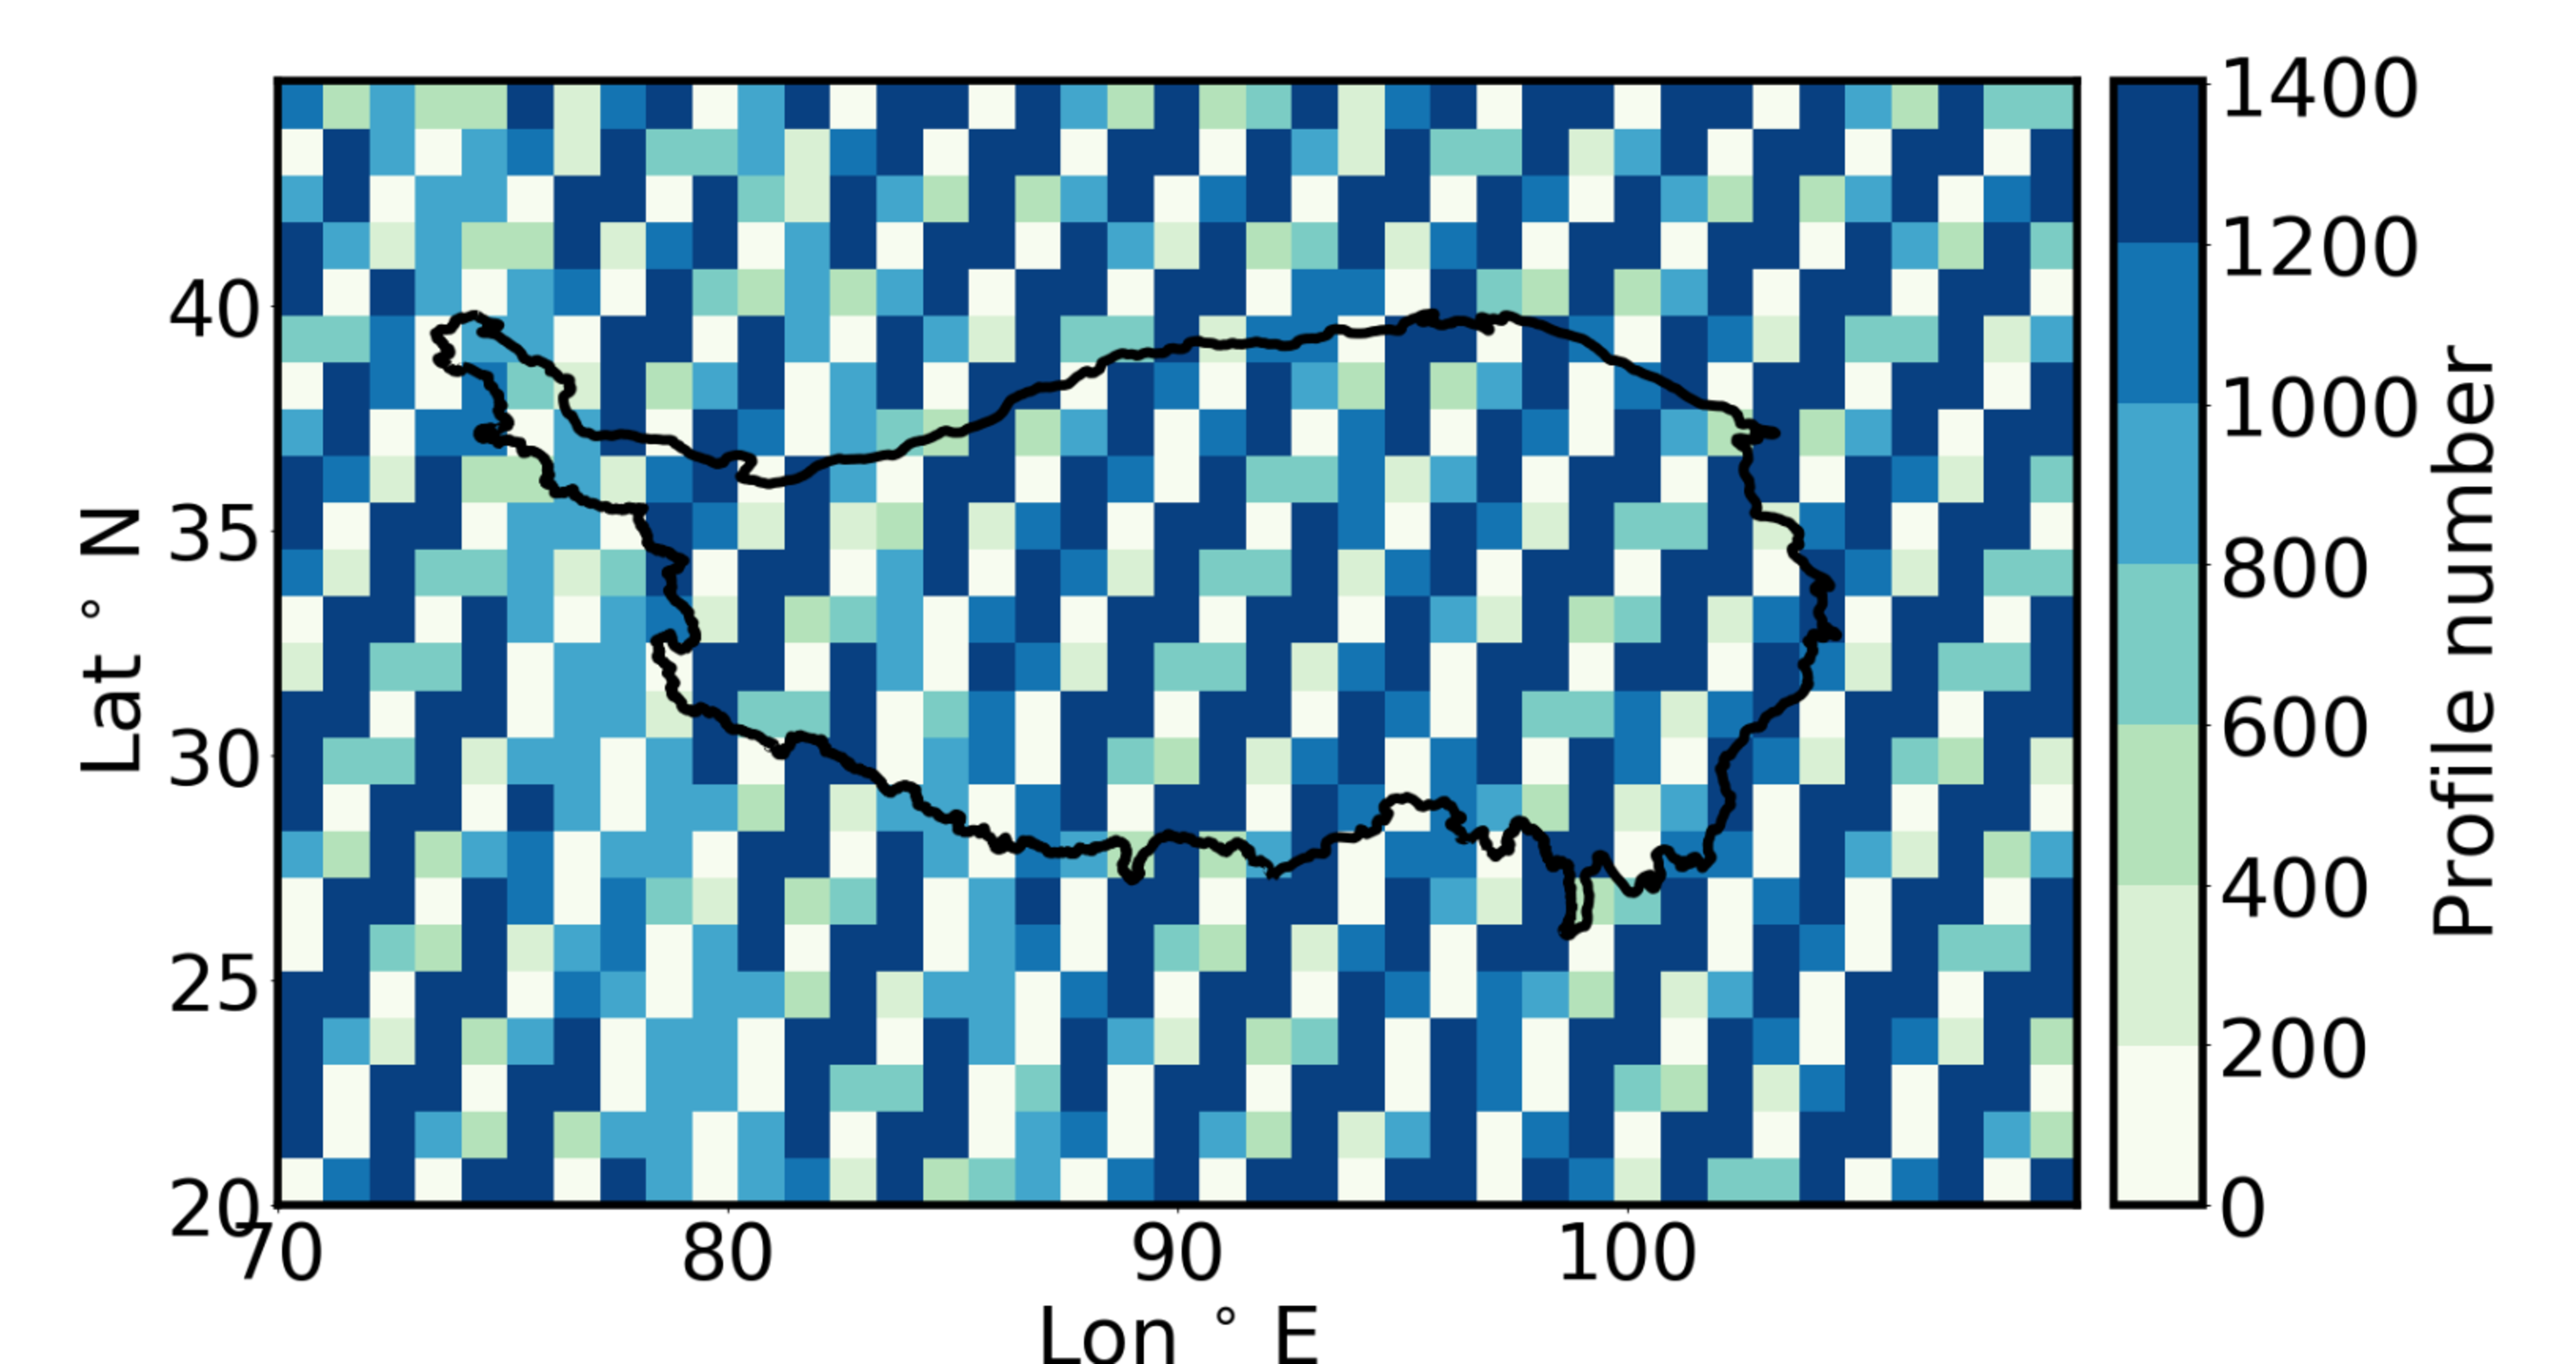
\includegraphics[width=0.5\textwidth]{mon_avg_profilenr.png}
\caption{Average number of monthly grid samples in 1$^{\circ}$ x 1$^{\circ}$ based on 2B-GEOPROF/2B-GEOPROF-LIDAR (2006 -- 2011). Grid cell values vary between a few and 1400. According to \citet{cu16}, the optimal compromise between profile sample amount per grid and an equal distribution over the grid cells is achieved in the 1$^{\circ}$ x 1$^{\circ}$ resolution grid.}
\label{fig:monthly_profiles}
%\end{minipage}
\end{wrapfigure}



Cloud fractions have been calculated as suggested by \citet{cl14}. In order to include hydrometeors that are only detected by \textit{CPR} or \textit{CALIOP}, the cloud fraction is set to 100 \%, when the \textit{CPR} cloud mask in 2B-GEOPROF is $>=$ 30 (corresponding to a high-confidence cloud detection) and when radar reflectivity is above the \textit{CPR} minimum detection level of -30 dBZ. Otherwise the value is replaced by the lidar fraction of hydrometors in one radar volume, as provided in the 2B-GEOPROF-LIDAR product (Table \ref{tab:data}). A profile is determined to be cloudy if it contains hydrometeor detections by either radar and/or lidar. Cloud layer occurrences refer, by contrast, only to vertically and horizontally connected cloud detections (cf. Section 2). Relative occurrence frequencies of cloud layer properties (e.g. cloud layer amount in Section 4.a  and ice cloud occurrences in Section 4.d) describe the average fractions of the respective parameter when a profile has been found to be cloudy. 



In order to identify regional differences of cloud characteristics within the TP and to account for the different impact of large-scale atmospheric circulation and associated moisture transport, a framework for regionalization introduced by \citet{cu13_2} has been used in this study. Since the hydro-climate of the TP is mainly affected by two atmospheric large-scale circulation patterns, namely the mid-latitude westerlies and the Indian and East Asian summer monsoon \citep{cu13_2, largescale2016}, the plateau is divided into three distinct zones based on ice core reconstructions \citep{cu13_2}. Whereas it is assumed that the domain north of latitude 35 $^{\circ}$N is primarily affected by the moisture transport through westerlies, the domain south of 30 $^{\circ}$N is, according to this framework, dominated by the monsoon circulation (Fig. \ref{fig:dem_tp_regimes}). The central TP between latitudes 30 $^{\circ}$N and 35 $^{\circ}$N is referred to as the transition zone and is affected by both large-scale circulation systems (Fig. \ref{fig:dem_tp_regimes}). It should also be noted, that only locations above 3000 m a.s.l. are defined as the TP. The study has further focused on the two seasons, where the respective large-scale circulation system prevail: (a) May -- September for the monsoon season \citep{monsoon_season_def2002} and (b) October -- April for the westerly season, which refers to the dry season between monsoon dissipation and onset, where the strongest midlatitudes westerlies occur \citep{largescale2016}.


\begin{figure}[!htbp]
%\begin{figure}[hbt]
\centering
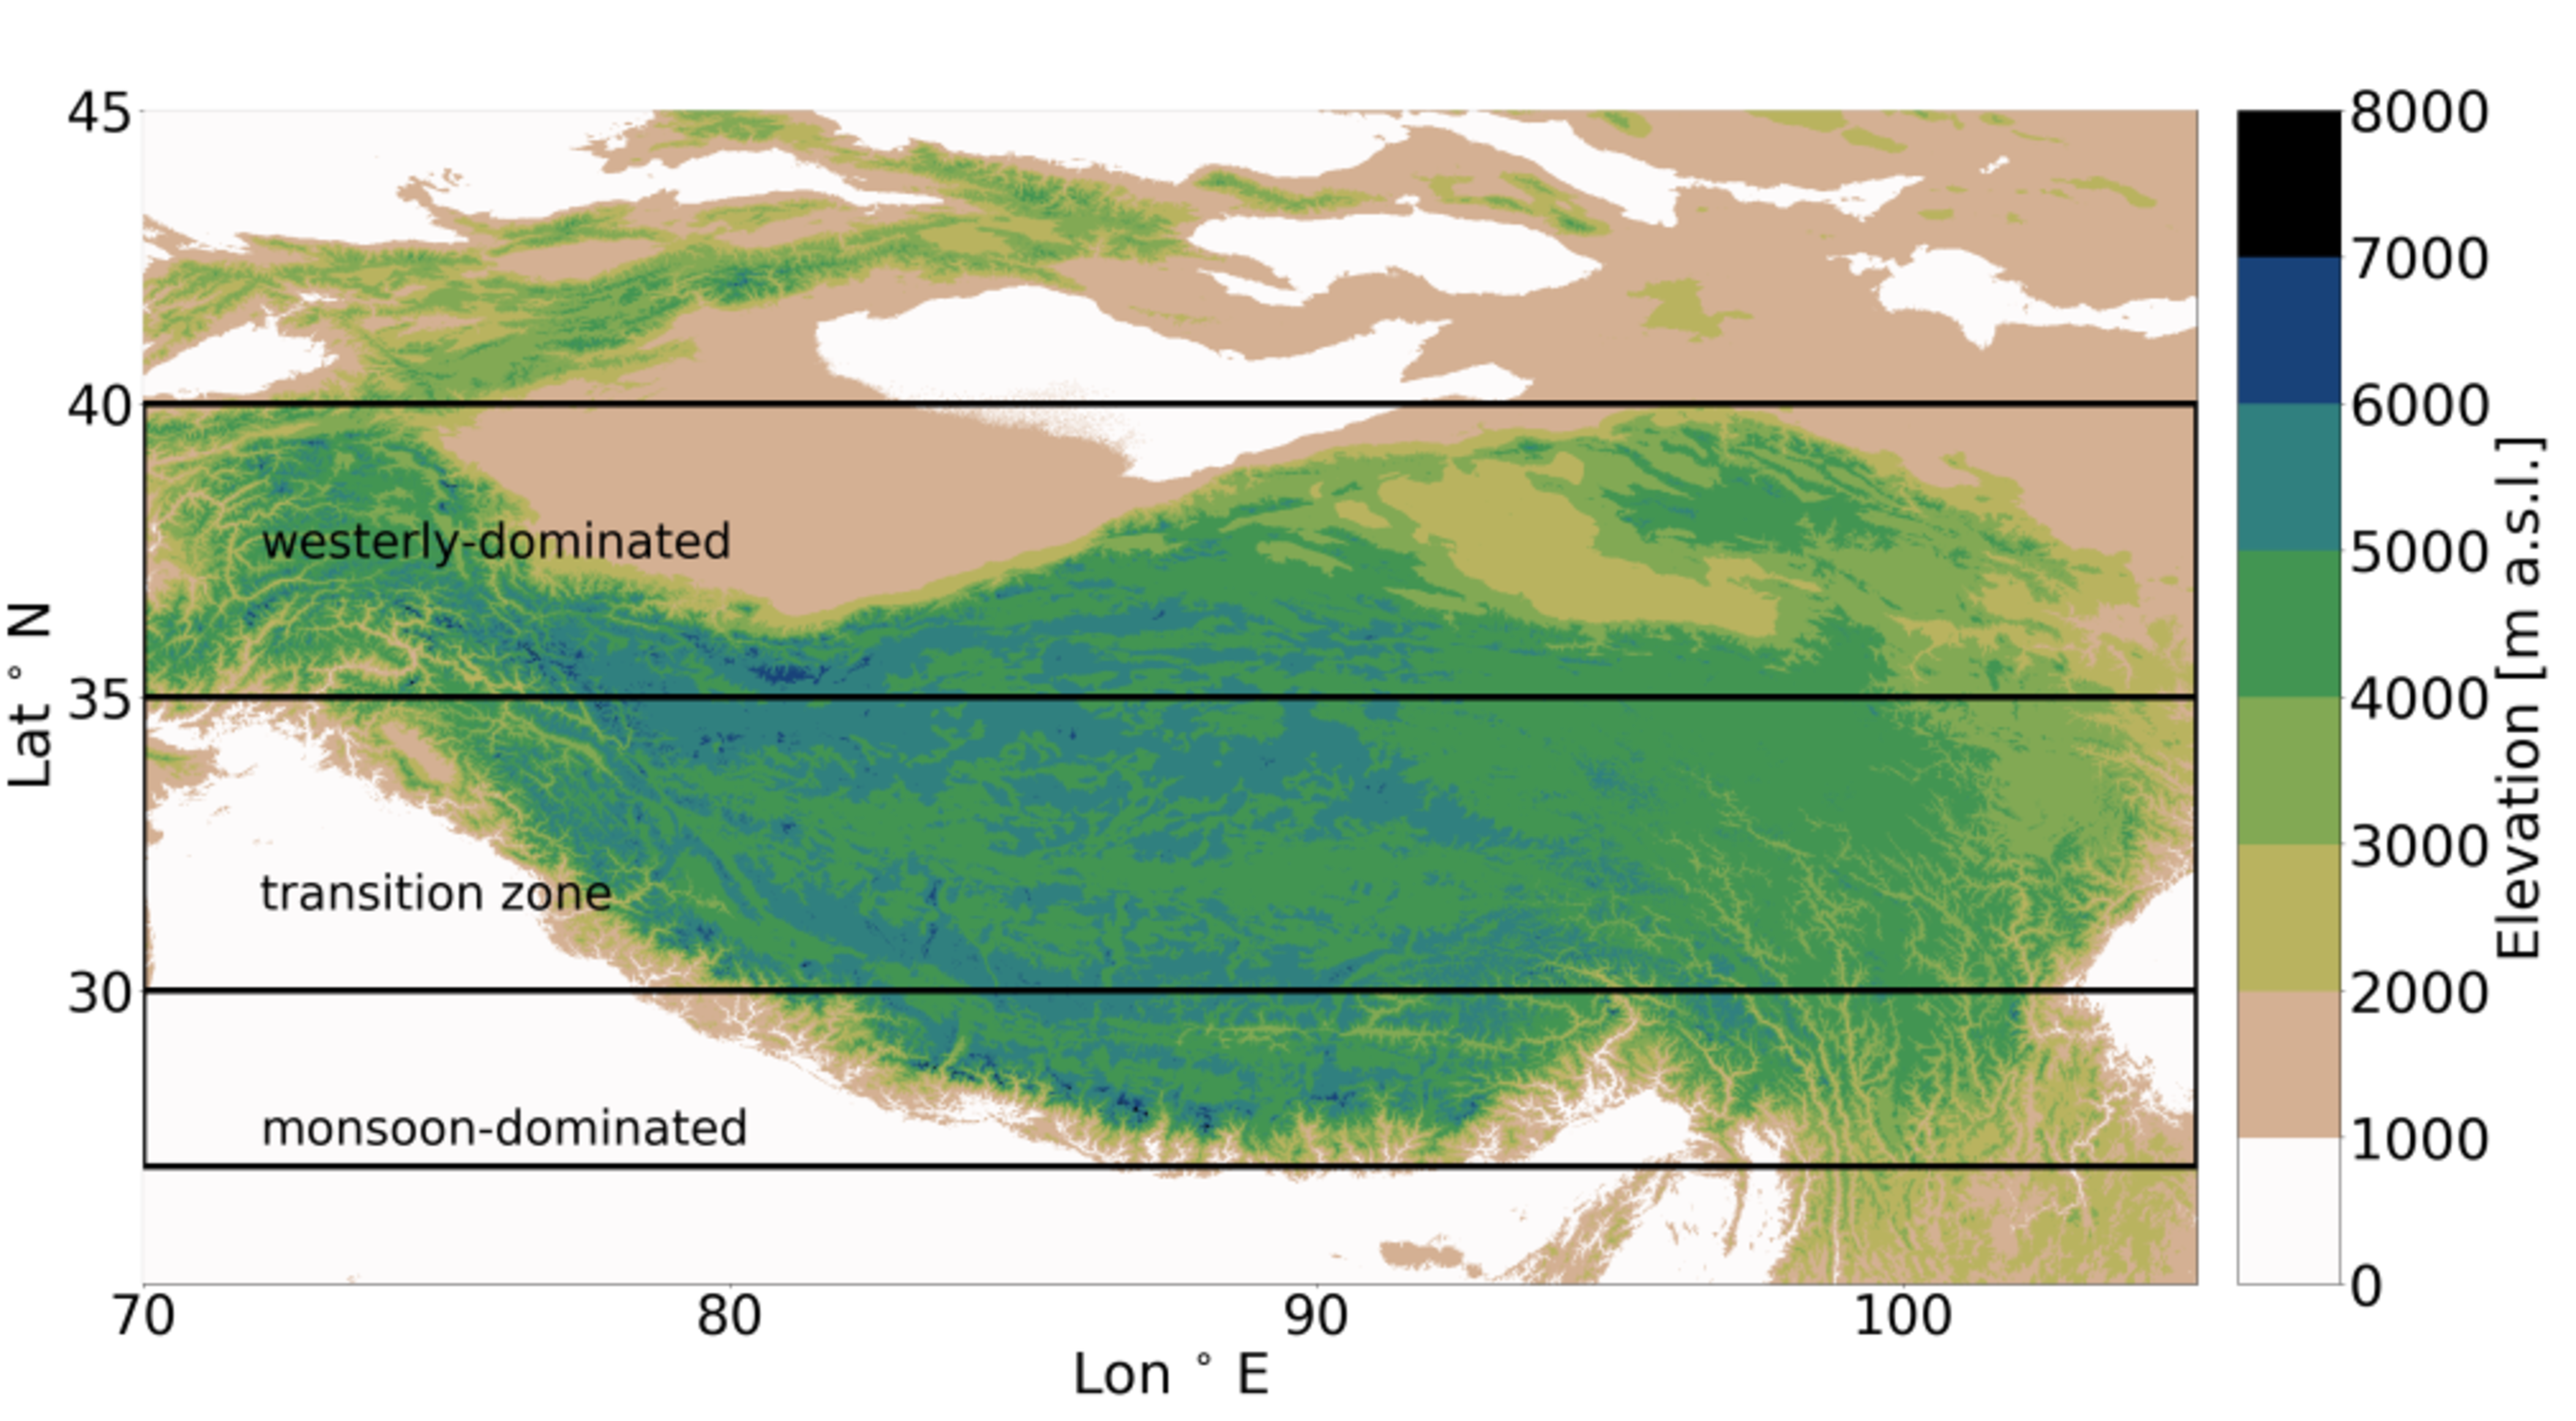
\includegraphics[width=0.6\textwidth]{DEM_TP_regimes.png}
\caption{Topography of the Tibetan Plateau (TP) and illustration of the three subregions based on impact of large-scale moisture transport according to \citet{cu13_2}. Locations within the domain 27 -- 40 $^{\circ}$N, 70 -- 105 $^{\circ}$E and above 3000 m a.s.l. are in this study defined as the TP.}
\label{fig:dem_tp_regimes}
%\end{figure}
\end{figure}


    
\section{Results}
\subsection{Total cloud occurrences and cloud types}

The gridded values for cloud occurrence frequencies (\%) over the TP are displayed in Figure \ref{fig:cloud_occ} for the monsoon season (May -- Sep) and westerly season (Oct -- Apr). Whereas most of the grid values exceed 70 \% for the monsoon months, the westerly season exhibits significantly lower values for all grid cells verifying that the plateau is much drier between October and April (Fig. \ref{fig:cloud_occ2}) than between May and September (Fig. \ref{fig:cloud_occ1}). Having said this, more than half of the sampled profiles are found to be cloudy during both seasons, indicating a generally high cloudiness over the whole region (Fig. \ref{fig:cloud_occ}). 

Table \ref{tab:profile_stats} shows the fractions of clouds detected in the datasets 2B-GEOPROF/2B-GEOPROF-LIDAR (2006 -- 2011) for each subregion, divided into daytime vs. nighttime and profiles with detected hydrometeors vs. cloud profiles with detected cloud layers. The respective fractions of cloud layer occurrences in the data products 2C-ICE and 2B-CLDCLASS-LIDAR are now shown, since these encompass a four-year (2007--2010) period which is already included in 2B-GEOPROF/2B-GEOPROF-LIDAR. The cloud detections differ hence at most 1 \% and show the same regional and diurnal variations as in 2B-GEOPROF/2B-GEOPROF-LIDAR . 
The table clarifies that the monsoon-dominated domain exhibits the highest percentages of detected clouds and cloud layers, followed by the westerly-dominated domain. In general, cloud and cloud layer occurrence frequencies are higher during daytime than during nighttime, whereby the largest day-night differences occur in the transition zone. 


\begin{figure}[!htbp]
\centering
    \begin{subfigure}[b]{0.5\textwidth}
       \centering
        \caption{monsoon}       
        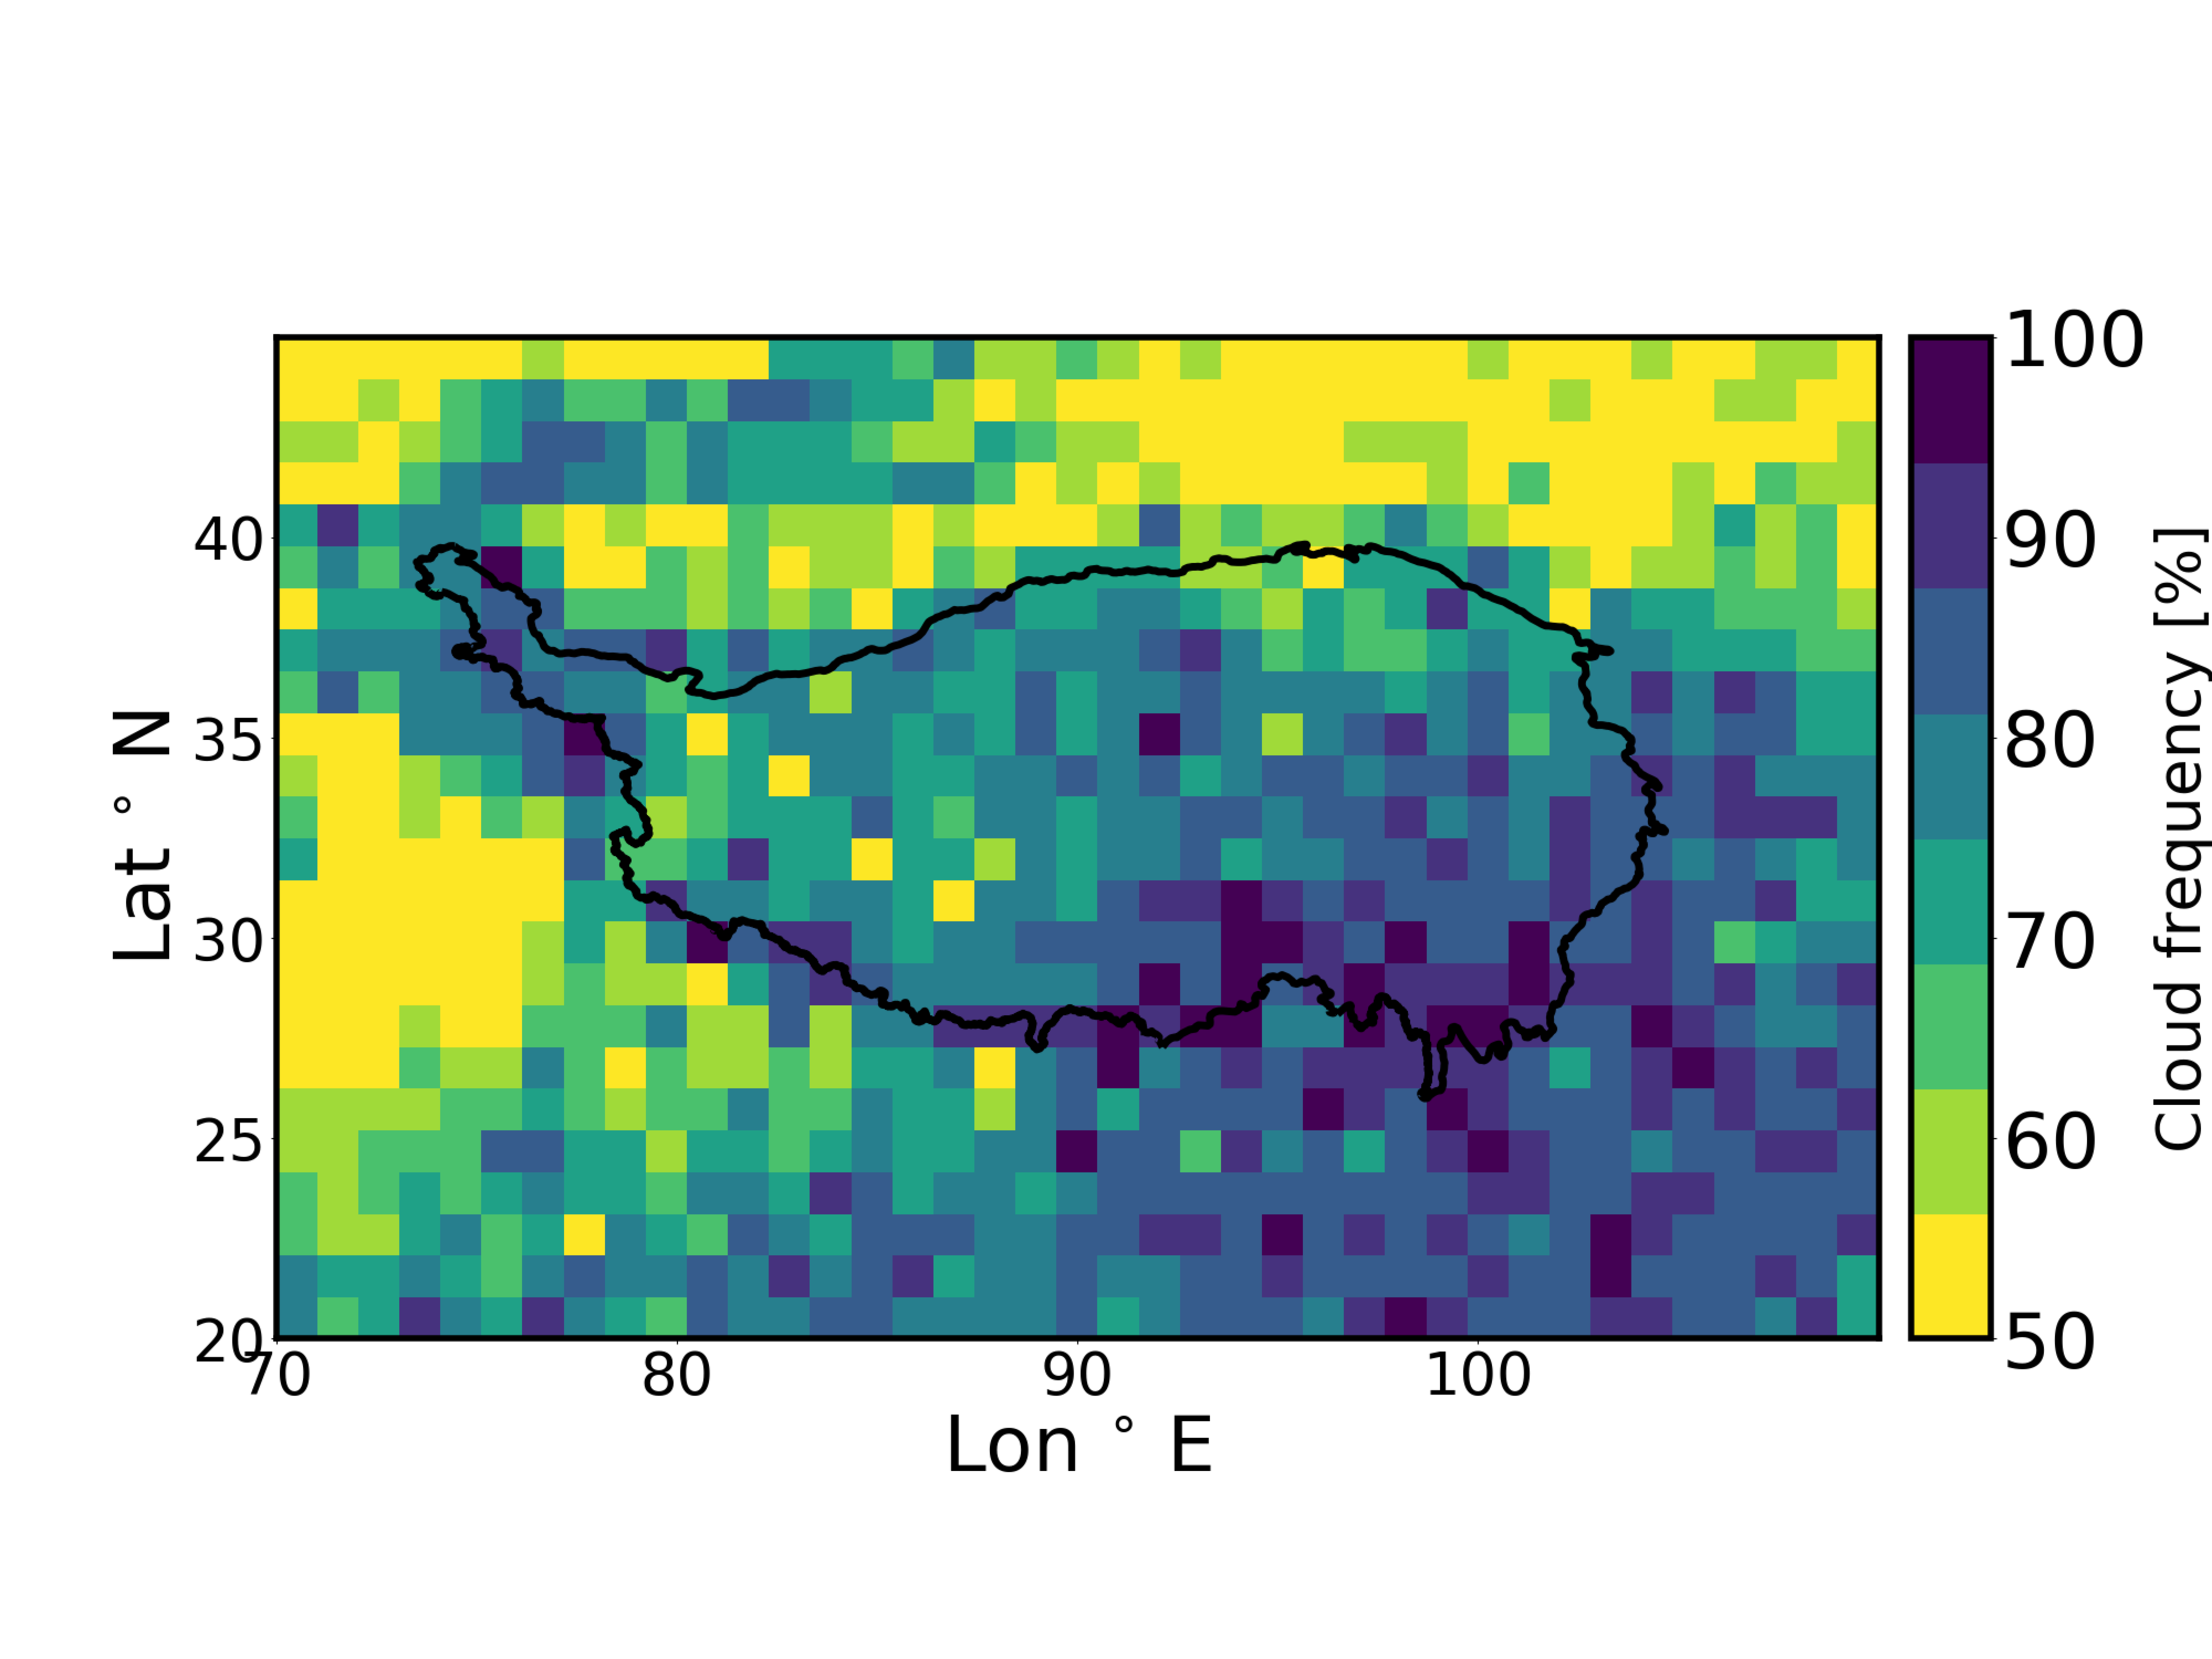
\includegraphics[width=\textwidth]{cloudfreq_monsoonseason.png}
        \label{fig:cloud_occ1}
    \end{subfigure}%
    \begin{subfigure}[b]{0.5\textwidth}
        \centering
        \caption{westerly} 
        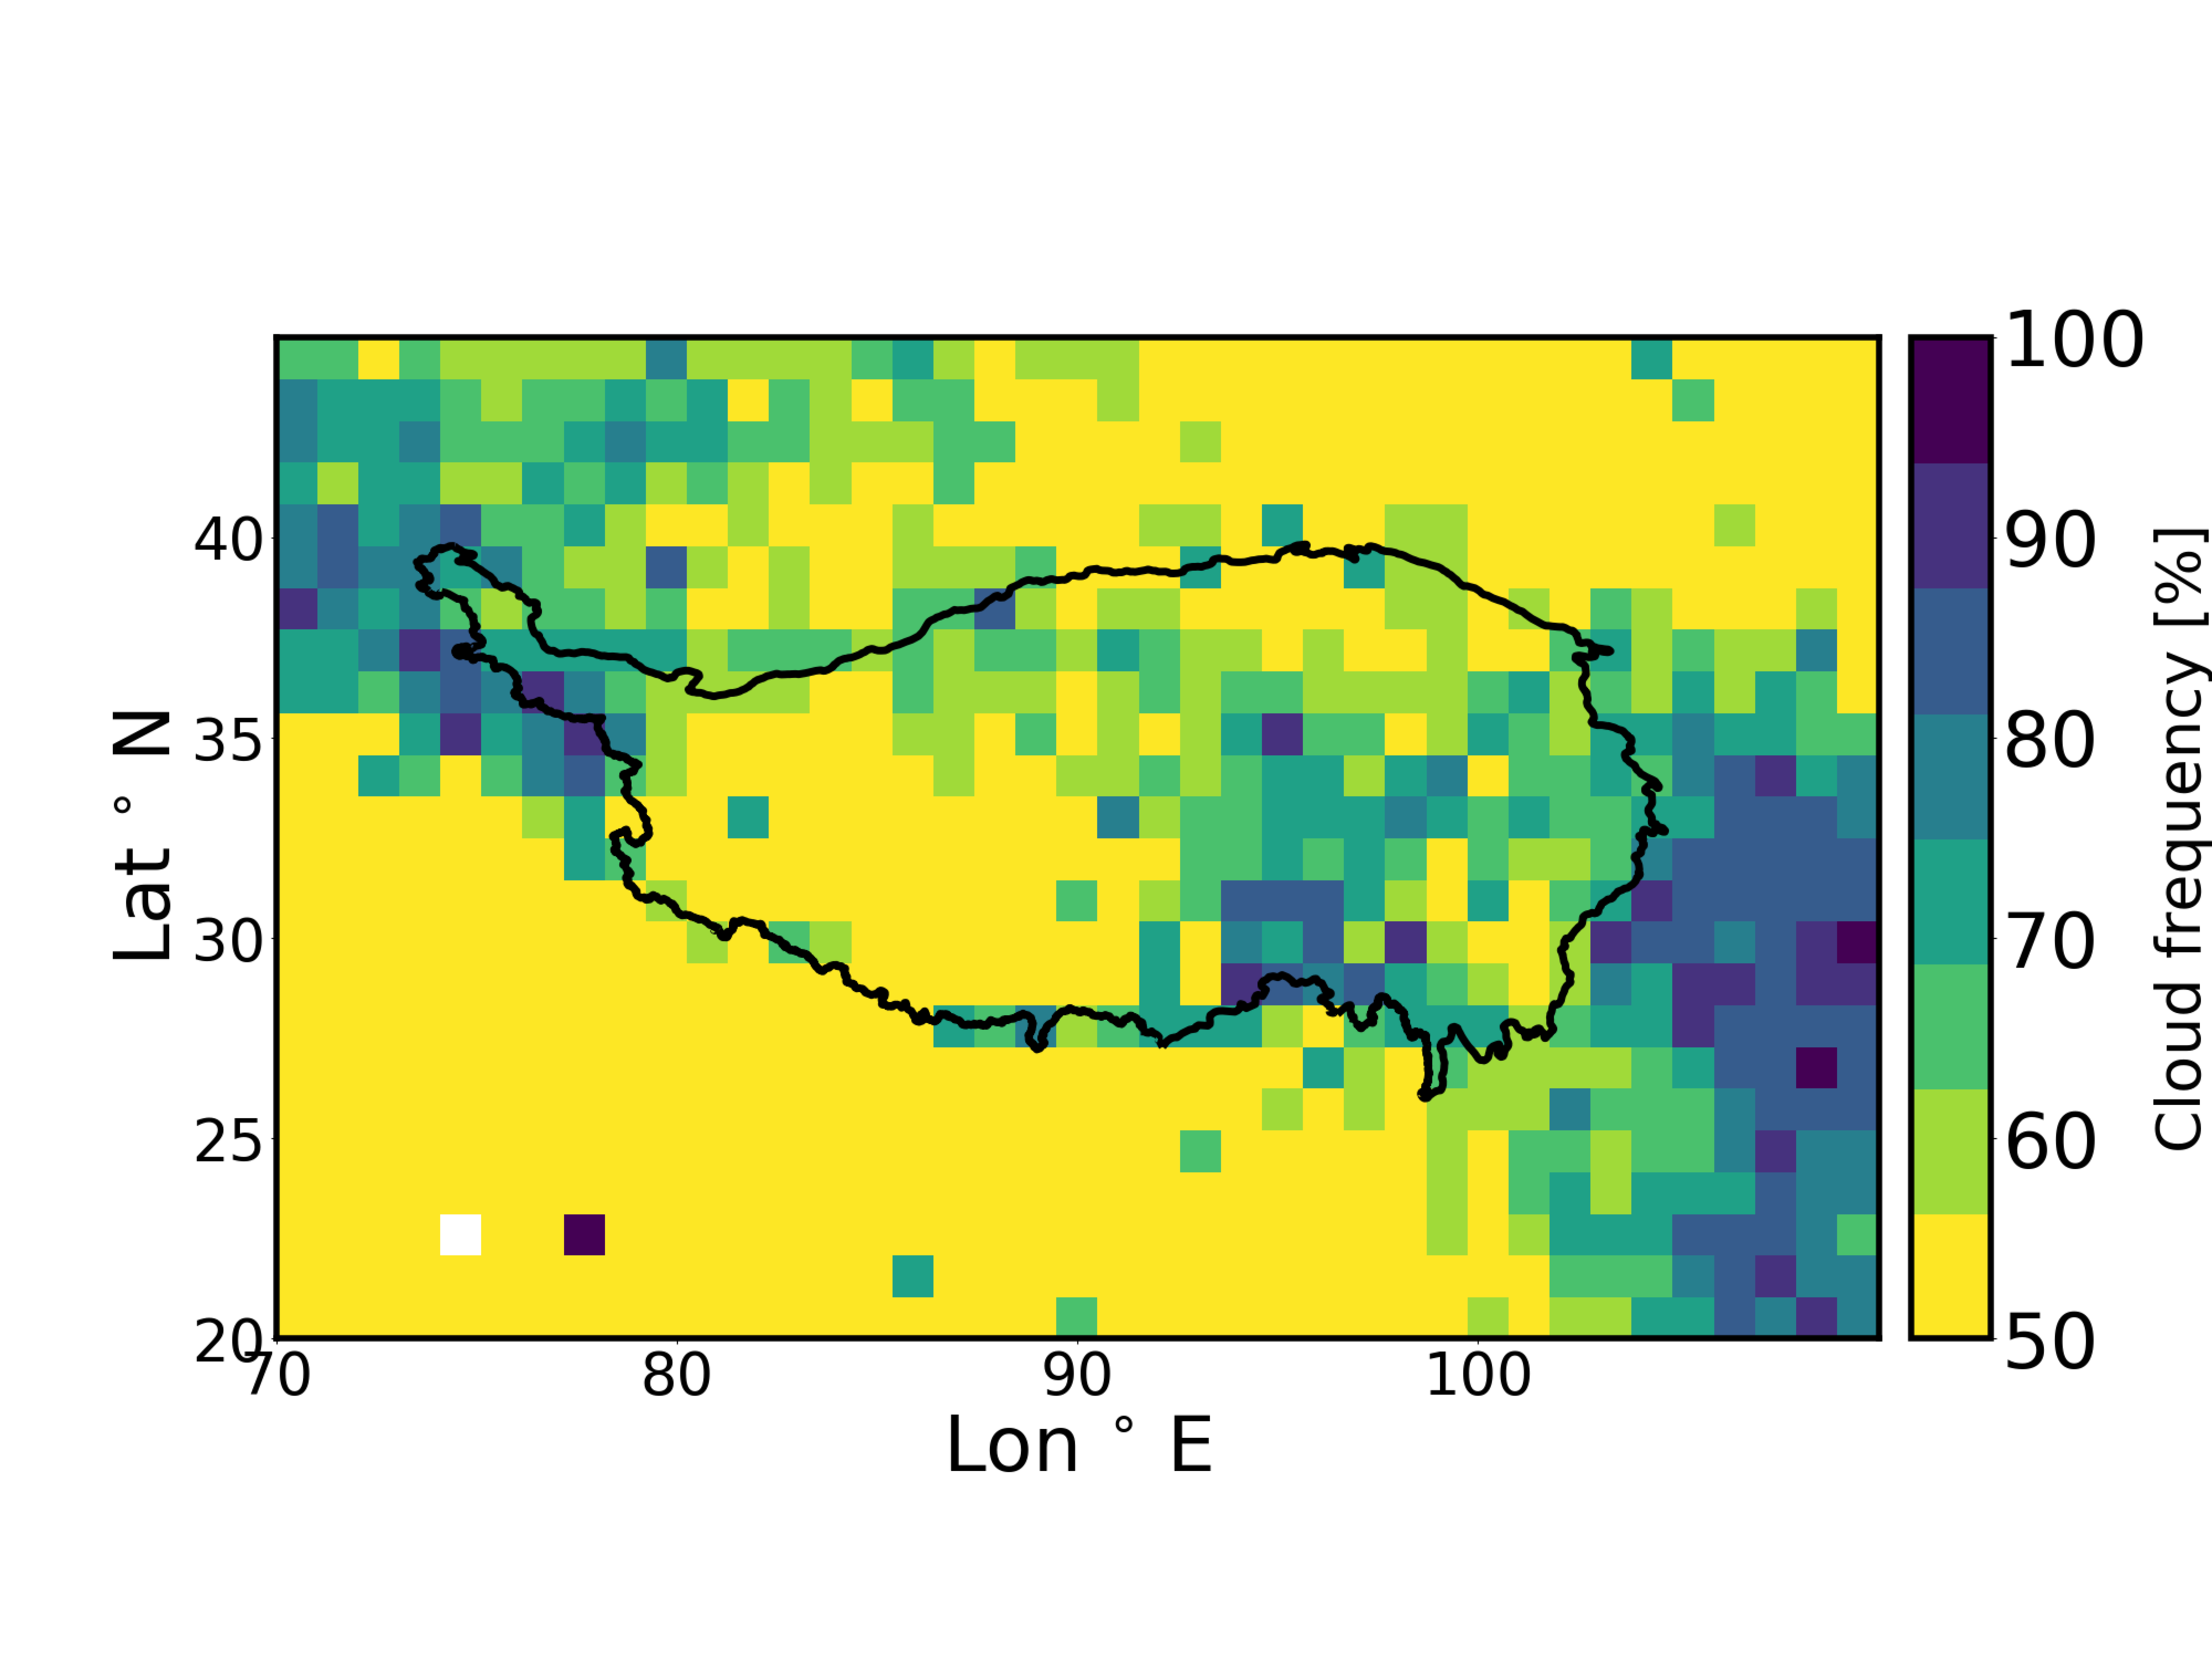
\includegraphics[width=\textwidth]{cloudfreq_westerlyseason.png}
         \label{fig:cloud_occ2}
    \end{subfigure}   
    \caption{Cloud occurrence frequencies (\%) over the TP for the (a) monsoon season (May -- Sep) and (b) westerly season (Oct -- Apr) based on 2B-GEOPROF and 2B-GEOPROF-LIDAR (2006 – 2011).}
    \label{fig:cloud_occ}
\end{figure}



Figure \ref{fig:cld_type} shows the occurrence frequencies (\%) for different types of detected cloud layers (in total 81 \% during the monsoon season and 64 \% during the westerly season) over the TP domain and the three subregions for the monsoon and westerly season based on 2B-CLDCLASS-LIDAR (2007 -- 2010). The most frequent cloud types over the TP and in all three subregions are As (Altostratus), Sc (Stratocumulus) and Cu (Cumulus, cumulus congestus), whereby As refer to non-precipitating cloud layers with base heights between 2 and 7 km above the surface and very little liquid water and Sc and Cu are clouds with base heights between 0 and 2 km above the surface \citep{cloudsat_classification}. Deep convective cloud layers (DC) occur only during the monsoon season and with frequencies below 3 \% in all three subregions. In general, stratiform cloud types (As and Sc) dominate the region, but show also a clear seasonality and differences between the subregions. Whereas As are the most frequent cloud type in the transition zone (Fig. \ref{fig:cld_type5} -- \ref{fig:cld_type6}) and the westerly-dominated domain (Fig. \ref{fig:cld_type7} -- \ref{fig:cld_type8}), Cu and Cr (Cirrus) are the most common cloud types in the monsoon-dominated domain (Fig. \ref{fig:cld_type3} -- \ref{fig:cld_type4}). The contribution of As in all subregions is generally higher during the westerly season (Fig. \ref{fig:cld_type2}, \ref{fig:cld_type4}, \ref{fig:cld_type6}, \ref{fig:cld_type8}) and about 15 \% higher for the entire TP domain compared to the monsoon season. The monsoon season is, by contrast, characterized by an increased contribution of Ac (Altocumulus) and Cr (Fig. \ref{fig:cld_type1}, \ref{fig:cld_type3}, \ref{fig:cld_type5}, \ref{fig:cld_type7}). 


\begin{figure}[!htbp]
    \begin{subfigure}[b]{0.5\textwidth}
       \centering
        \caption{TP, May -- Sep}
        \includegraphics[width=\textwidth]{cld_type_freq_TP_monsoonseason.png}
        \label{fig:cld_type1}

    \end{subfigure}%
    ~ 
        \begin{subfigure}[b]{0.5\textwidth}
       \centering
        \caption{TP, Oct -- Apr}
        \includegraphics[width=\textwidth]{cld_type_freq_TP_westerlyseason.png}
\label{fig:cld_type2}
    \end{subfigure}%
    
    \bigskip
   
    \begin{subfigure}[b]{0.5\textwidth}
        \centering
        \caption{monsoon-dominated, May -- Sep}        
        \includegraphics[width=\textwidth]{cld_type_freq_monsoondomain_monsoonseason.png}
        \label{fig:cld_type3}
    \end{subfigure} 
    ~
    \begin{subfigure}[b]{0.5\textwidth}
        \centering
        \caption{monsoon-dominated, Oct -- Apr }        
        \includegraphics[width=\textwidth]{cld_type_freq_monsoondomain_westerlyseason.png}
        \label{fig:cld_type4}
    \end{subfigure}%
    
    \bigskip 
    
    \begin{subfigure}[b]{0.5\textwidth}
        \centering
        \caption{transition zone, May -- Sep }        
        \includegraphics[width=\textwidth]{cld_type_freq_transitionzone_monsoonseason.png}
        \label{fig:cld_type5}
        \end{subfigure}
        ~ 
        \begin{subfigure}[b]{0.5\textwidth}
        \centering
        \caption{transition zone, Oct -- Apr }        
        \includegraphics[width=\textwidth]{cld_type_freq_transitionzone_westerlyseason.png}
        \label{fig:cld_type6}
        \end{subfigure}
        \end{figure}
        
 \begin{figure}\ContinuedFloat   
        \begin{subfigure}[b]{0.5\textwidth}
        \centering
        \caption{westerly-dominated, May -- Sep }        
        \includegraphics[width=\textwidth]{cld_type_freq_westerlydomain_monsoonseason.png}
        \label{fig:cld_type7}
        \end{subfigure}
        ~ 
        \begin{subfigure}[b]{0.5\textwidth}
        \centering
        \caption{westerly-dominated, Oct -- Apr }        
        \includegraphics[width=\textwidth]{cld_type_freq_westerlydomain_westerlyseason.png}
        \label{fig:cld_type8}
        \end{subfigure}  
        \caption{Relative occurrence frequencies (\%) of different cloud types for TP domain (a -- b), monsoon-dominated domain (c --d ), transition zone (e -- f) and westerly-dominated domain (g -- h) during the monsoon (May -- Sep) and westerly season (Oct -- Apr), based on 2B-CLDCLASS-LIDAR (2007 -- 2010). The acronyms stand for following cloud types: Cr = Cirrus, As = Altostratus, Ac = Altocumulus, St = Stratus, Sc= Stratocumulus, Cu = Cumulus, Ns = Nimbusstratus, DC= deep convection (layer base above 3 km above surface and large vertical extent), CLD = total cloud layer amount.}
\label{fig:cld_type}
\end{figure}


\subsection{Cloud vertical structure}

The monthly variation of vertical cloud fractions based on 2B-GEOPROF/2B-GEOPROF-LIDAR (2006 -- 2010), as shown in Figure \ref{fig:vertical_cloudfract},  highlight once again the strong seasonality of cloud occurrences and indicate that the highest cloud fractions over the TP domain occur between 8 and 10 km a.s.l. from February to April and between 5 and 8 km a.s.l. during the monsoon season from May to September. This shows that the summer months are characterized by stronger cloud signals at lower levels above mean sea level, compared to the spring months where the troposphere above the TP is marked by hydrometeors at higher heights. The fact that the transition zone exhibits characteristics of both domains (Fig. \ref{fig:vertical_cloudfract5}-- \ref{fig:vertical_cloudfract6}) together with the spring peak of cloud fractions in the westerly-dominated domain (Fig. \ref{fig:vertical_cloudfract7}-- \ref{fig:vertical_cloudfract8}) verify that the applied regional framework of \citet{cu13_2}, implying precipitation peaks during spring in the northern TP, is reflected in the data. Day-night differences are most obvious in the monsoon-dominated domain, where high-level cloud fractions increase significantly during nighttime between June and August (Fig. \ref{fig:vertical_cloudfract3} -- \ref{fig:vertical_cloudfract4}). The two maxima of cloud fractions (5 -- 8 km and 12 -- 15 km a.s.l.) are disconnected, suggesting that the cloud peaks are associated with different cloud layer types rather than deep convective cells (Fig. \ref{fig:vertical_cloudfract4}). Recalling the retrieved cloud types for the monsoon-dominated domain during summer, this indicates the simultaneous occurrences of cirrus and lower convective clouds with small to moderate vertical extent. 


It should be noted that the higher cloud fractions in the upper troposphere during nighttime do not depict that cloud layers or profiles containing hydrometeors are more frequent during night. Indeed, the opposite was found to be true (cf. sec. 4.1), so the higher cloud fractions during night reflect rather that \textit{CPR}-detected hydrometeors and hence precipitation are more frequent (cf. sec. 3), but that the radar signals are detected from a smaller amount of cloudy profiles. 


\begin{figure}[!htbp]
\centering
    \begin{subfigure}[b]{0.5\textwidth}
       \centering
        \caption{TP, daytime}
        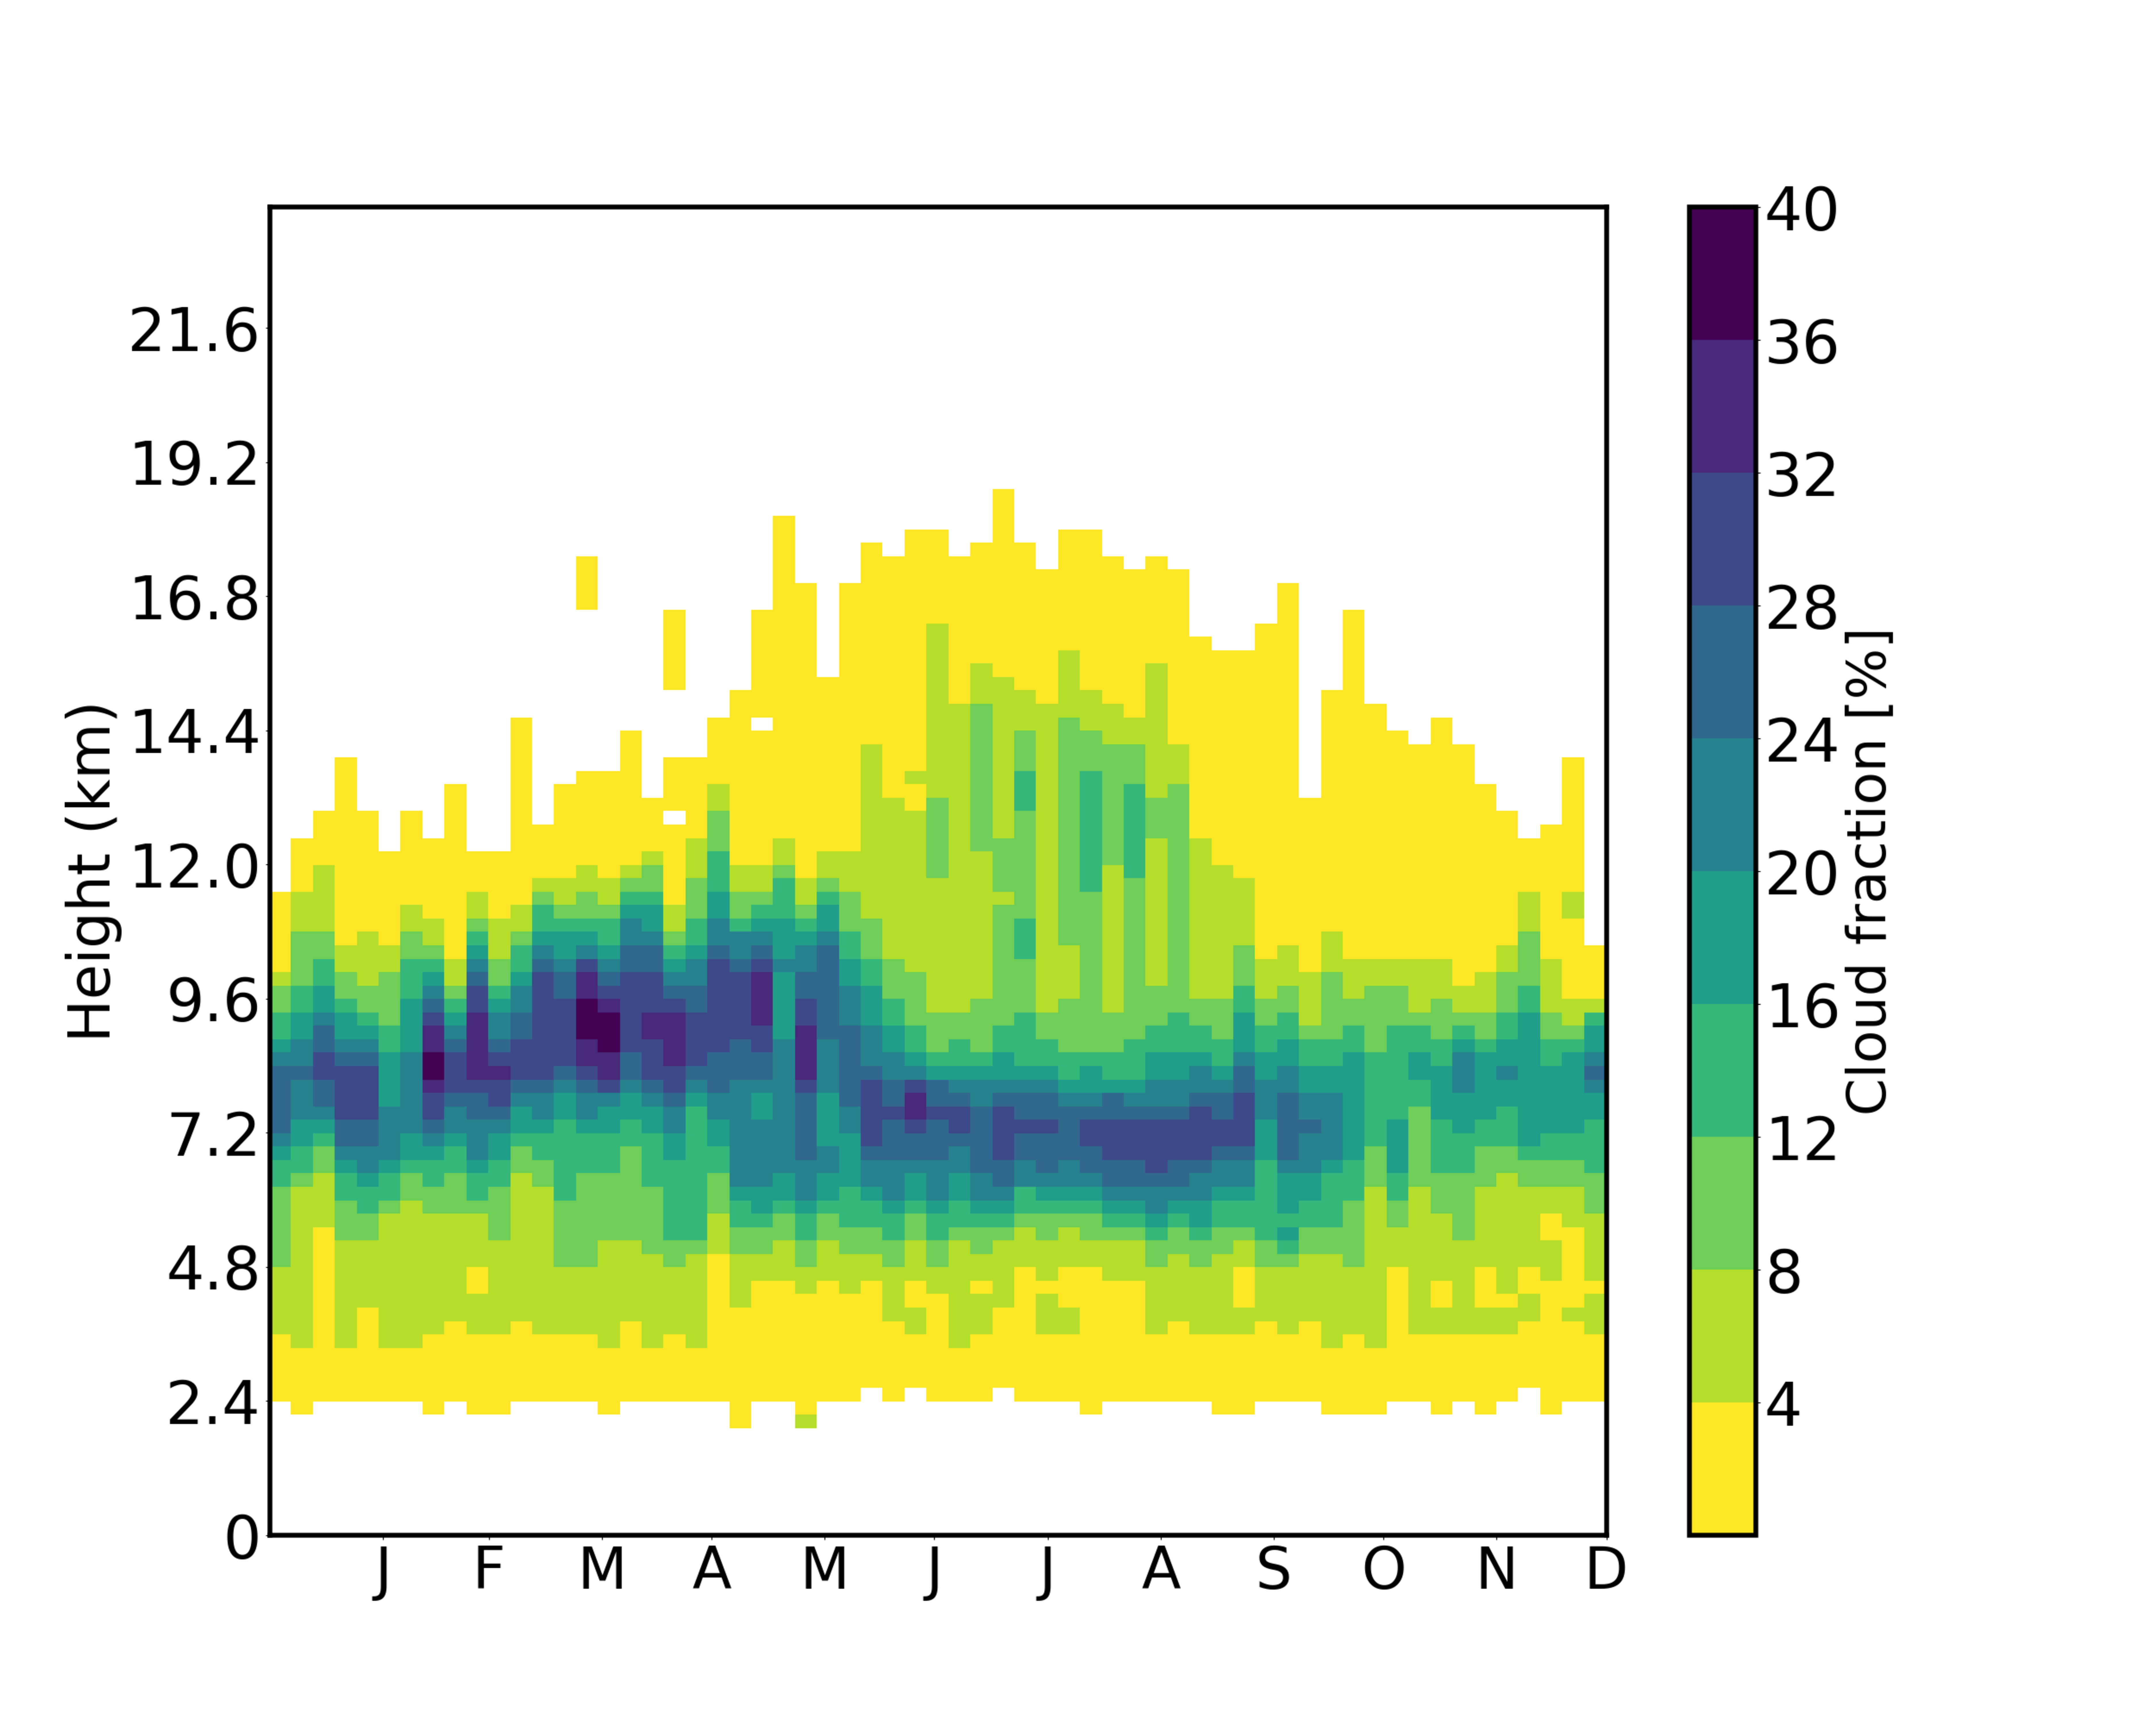
\includegraphics[width=\textwidth]{cloudsat_cloudfract_seasonal_pentadavg_day.png}
        \label{fig:vertical_cloudfract1}
    \end{subfigure}%
    ~ 
    \begin{subfigure}[b]{0.5\textwidth}
        \centering
        \caption{TP, nighttime}        
        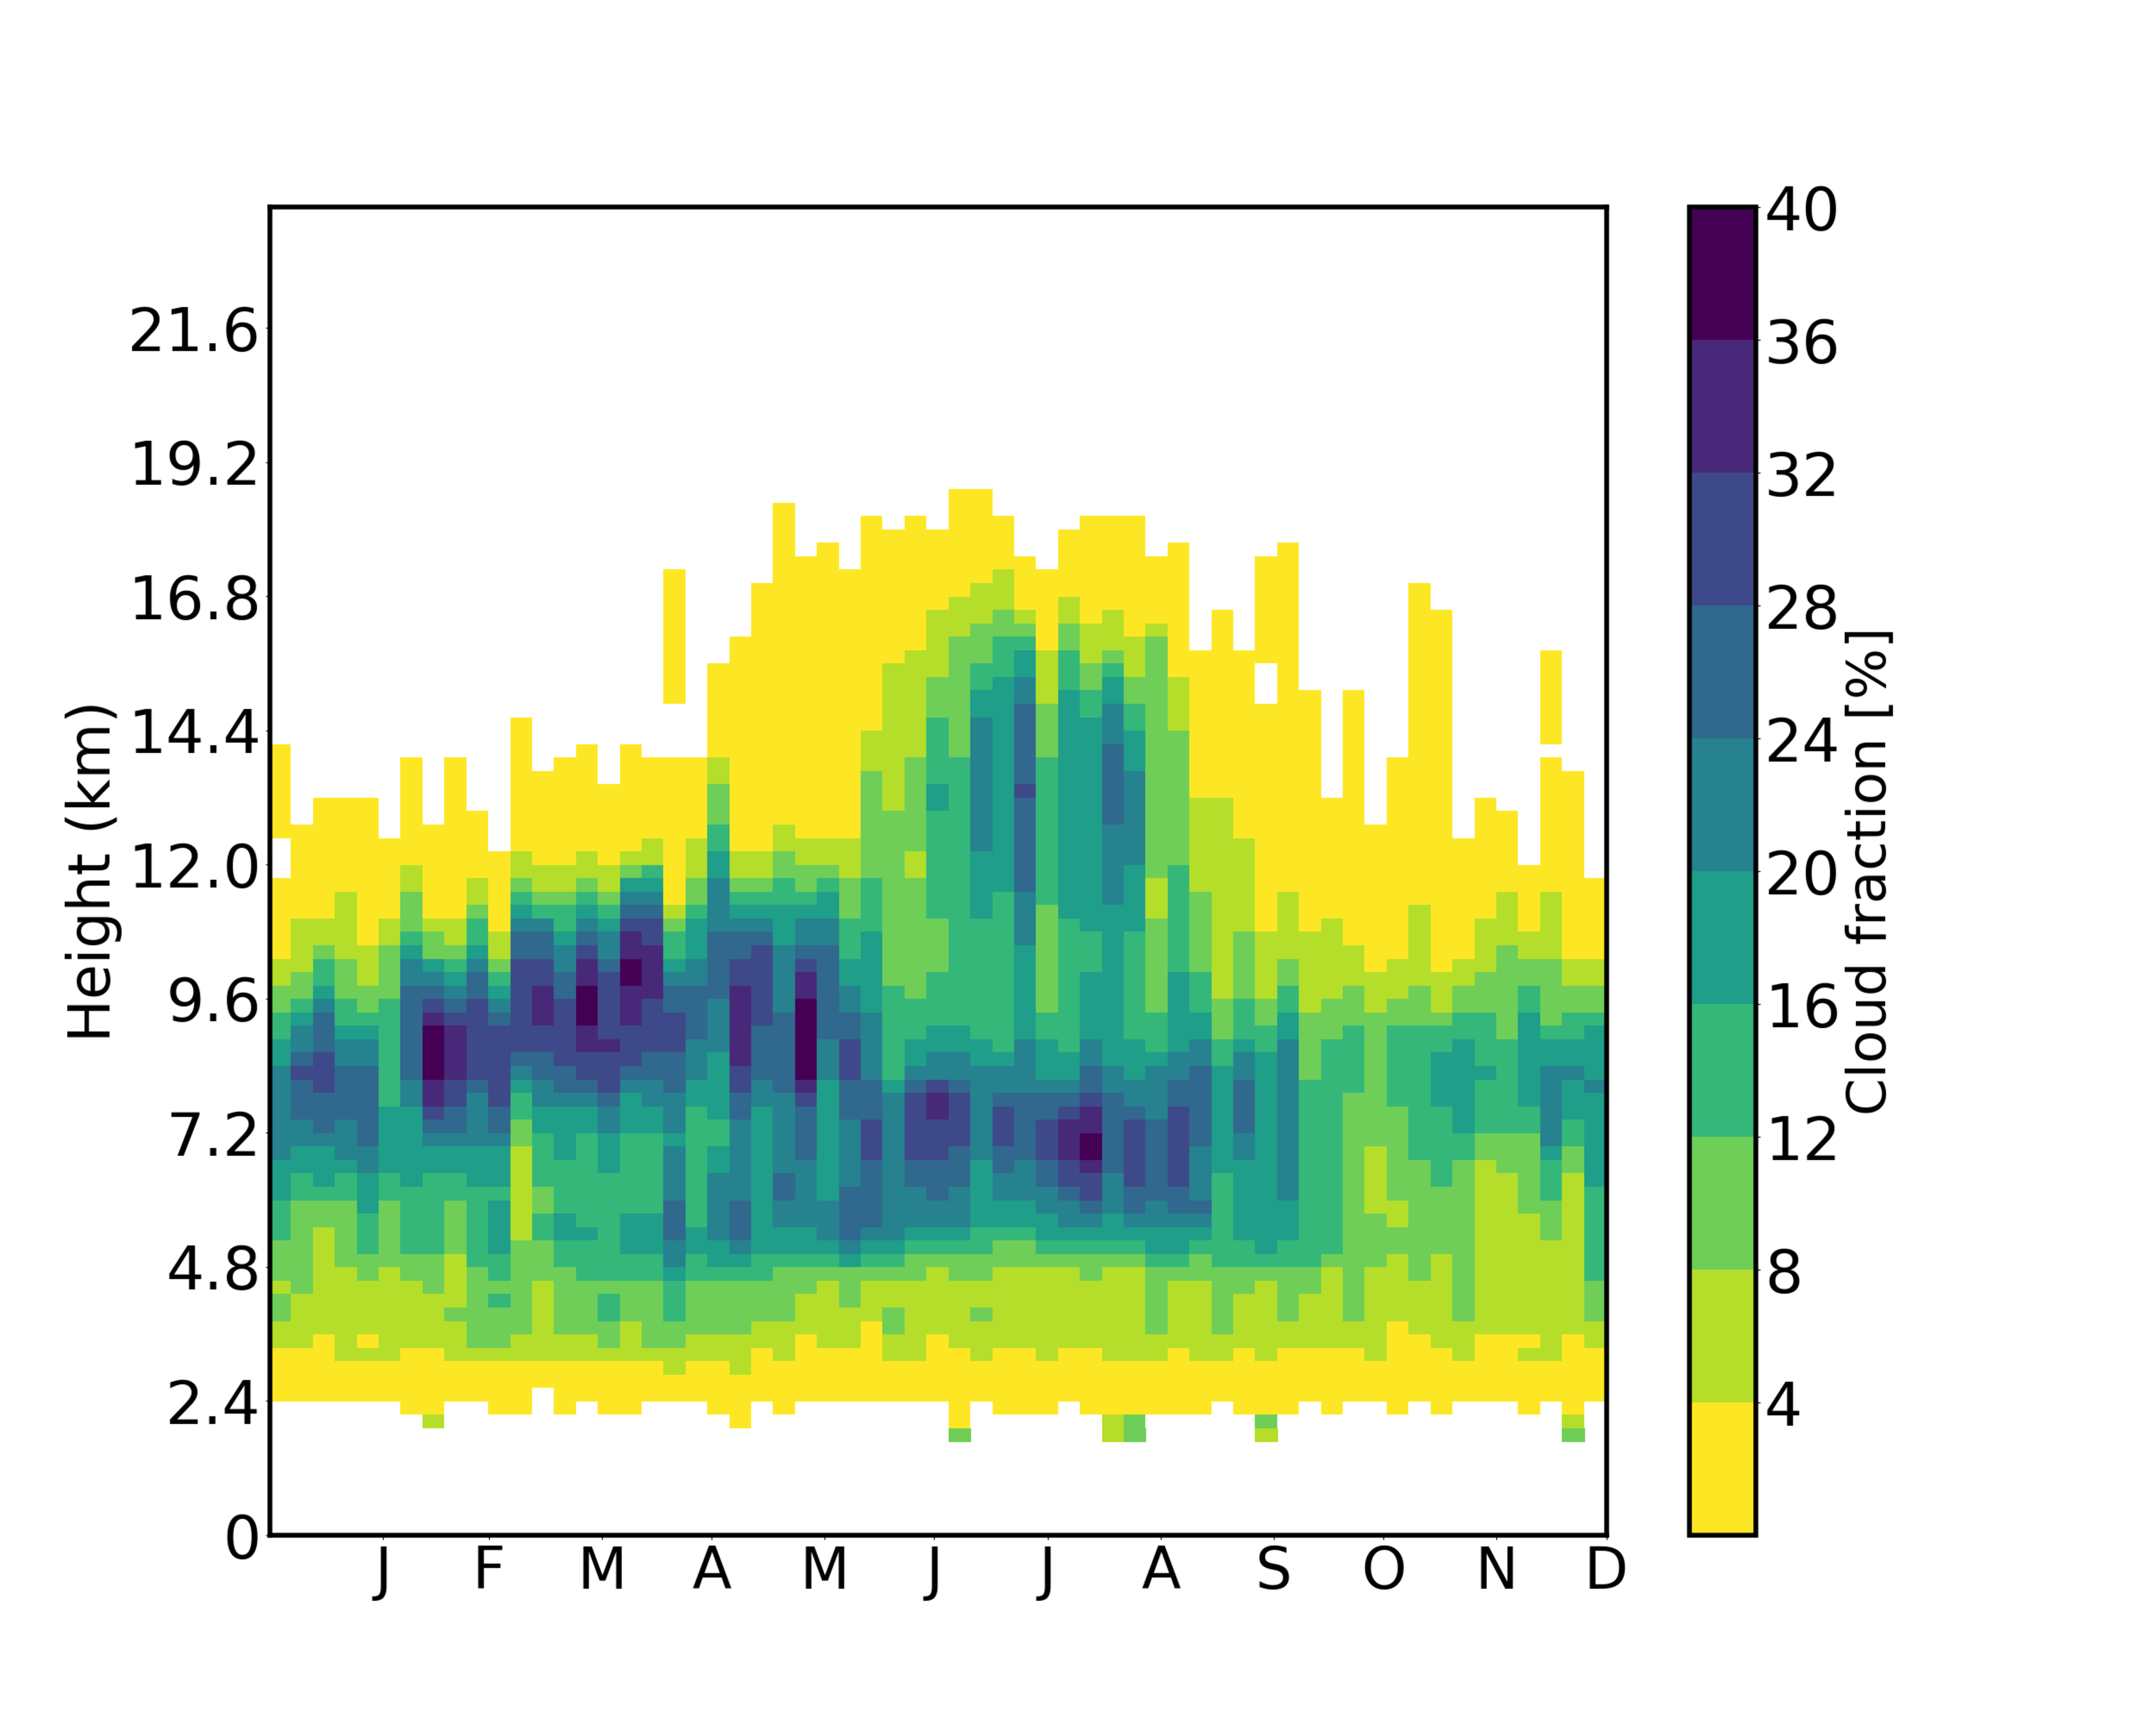
\includegraphics[width=\textwidth]{cloudsat_cloudfract_seasonal_pentadavg_night.png}
        \label{fig:vertical_cloudfract2}

    \end{subfigure}
    
    \bigskip

    \begin{subfigure}[b]{0.5\textwidth}
        \centering
        \caption{monsoon-dominated, daytime }        
        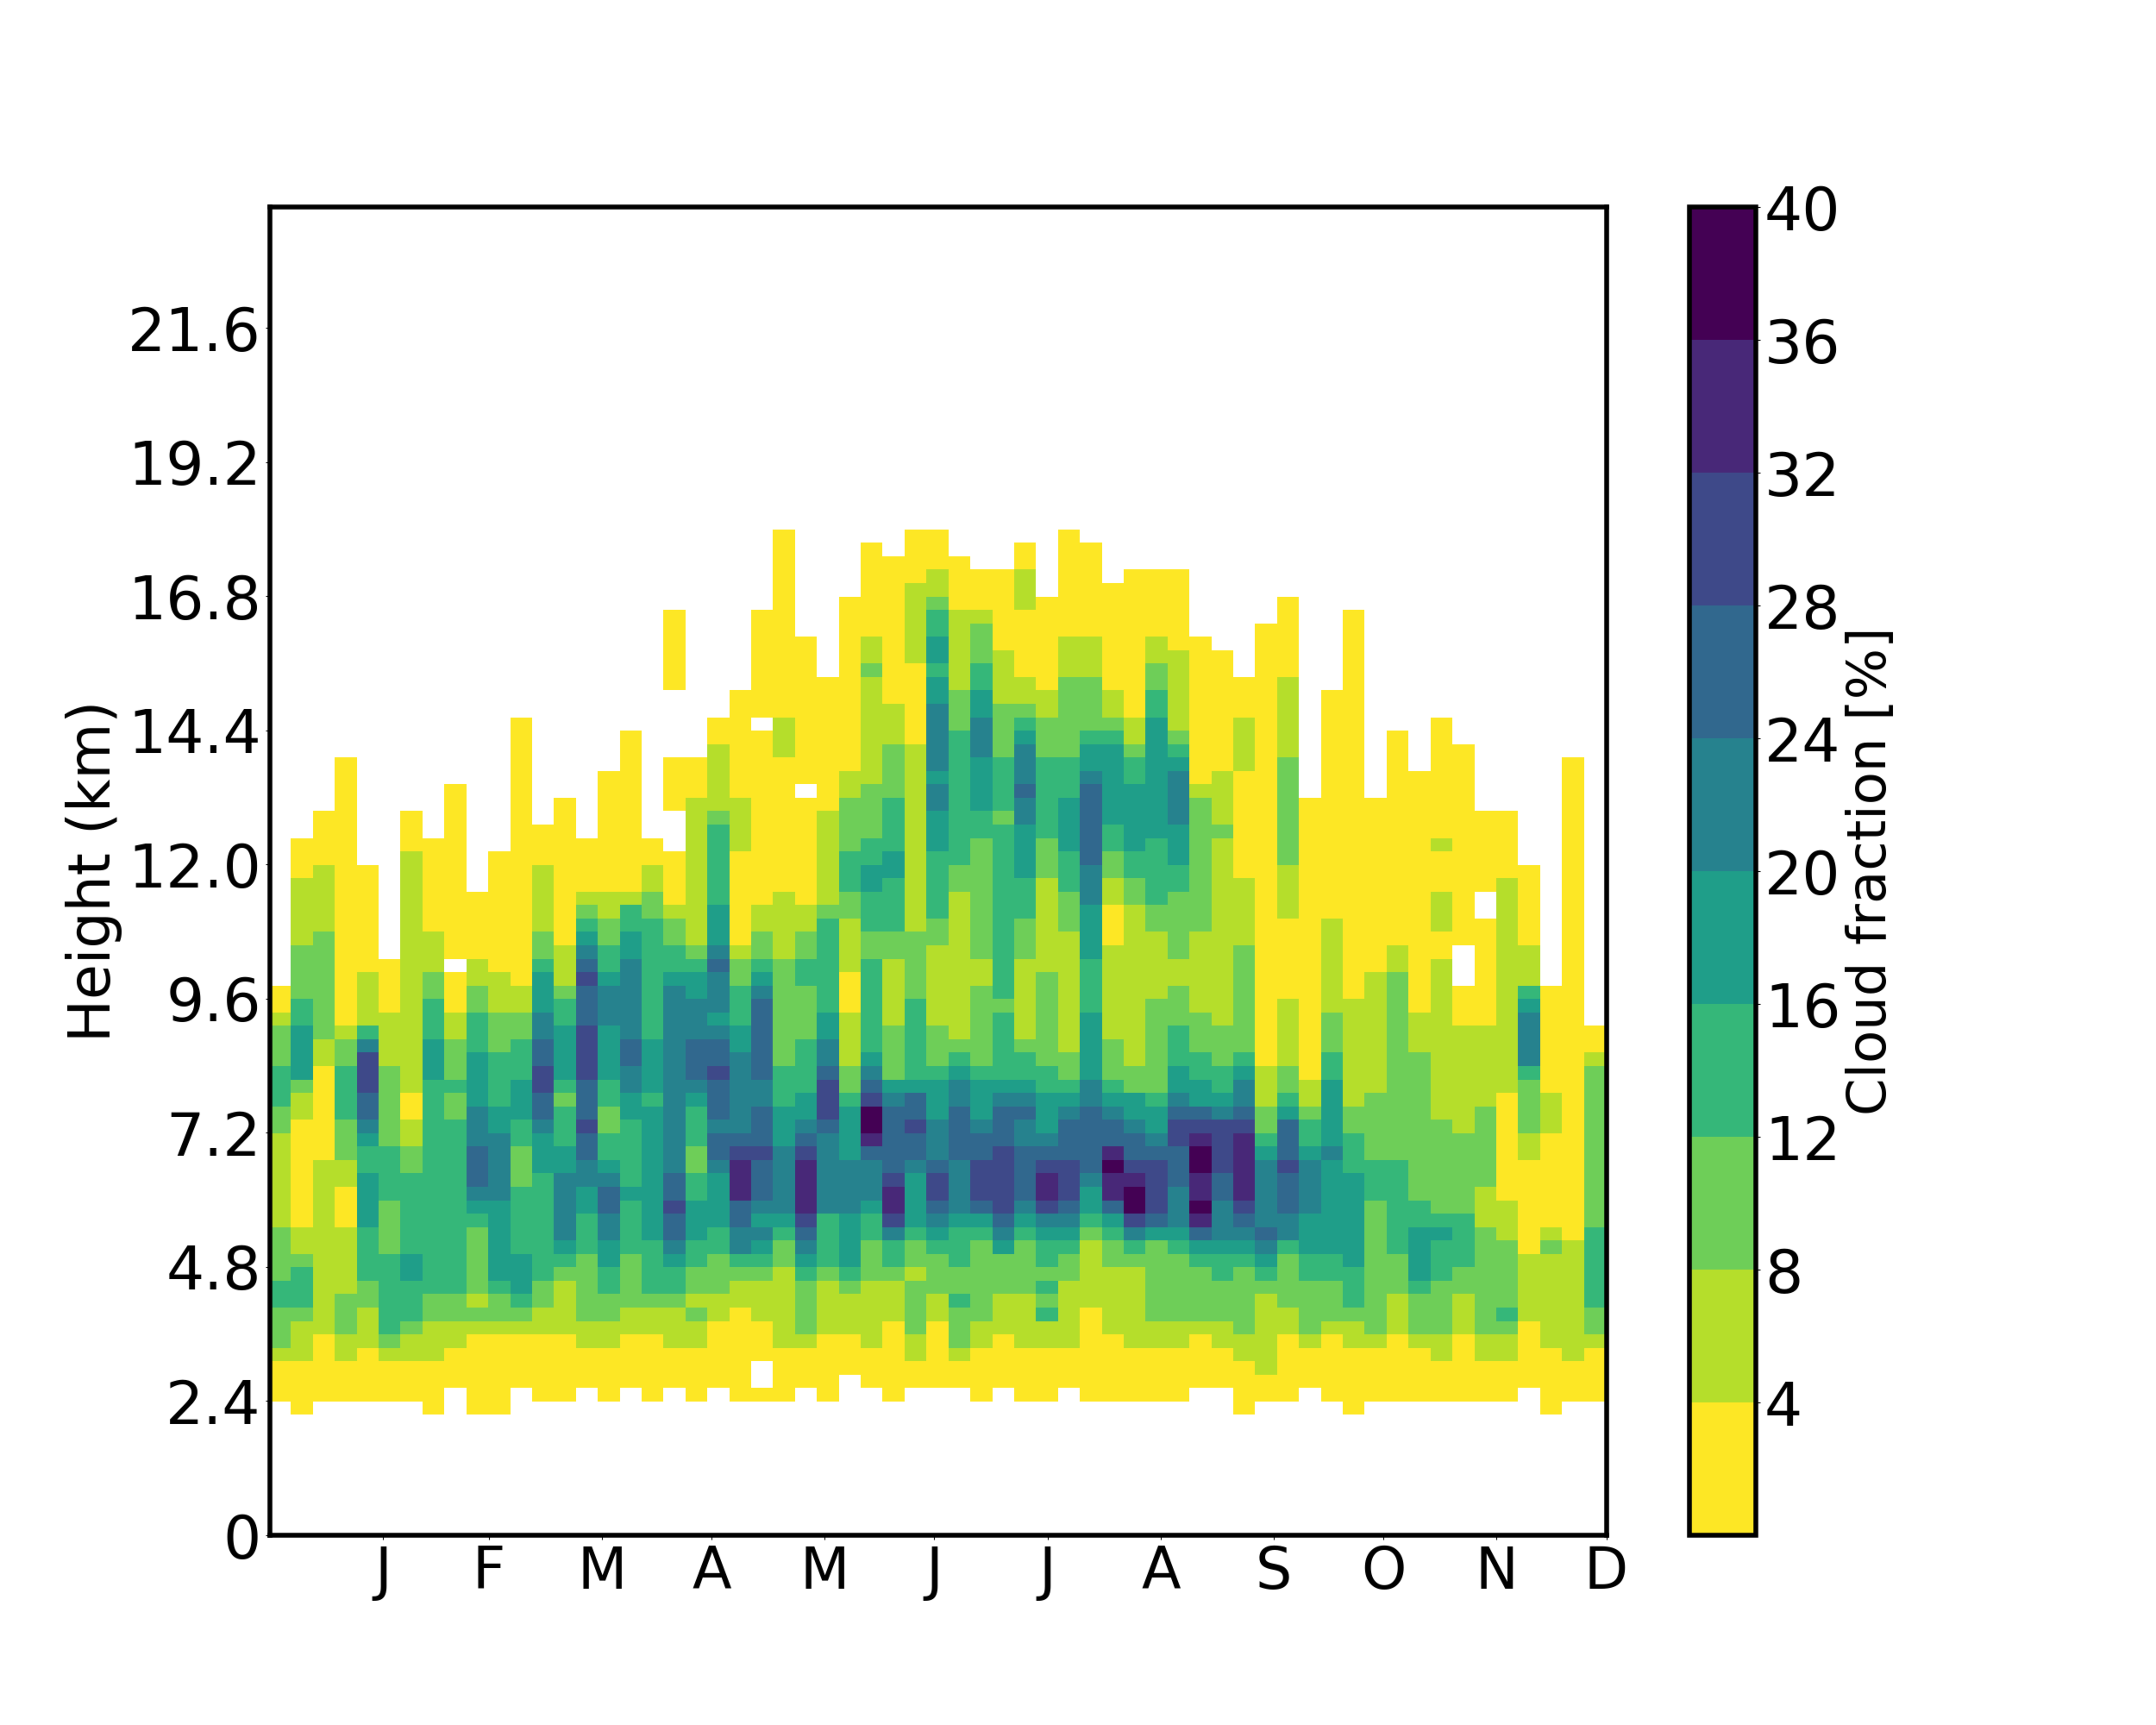
\includegraphics[width=\textwidth]{cloudsat_cloudfract_seasonal_monsoonmode_day.png}
        \label{fig:vertical_cloudfract3}

    \end{subfigure}%
    ~ 
    \begin{subfigure}[b]{0.5\textwidth}
        \centering
        \caption{monsoon-dominated, nighttime }        
        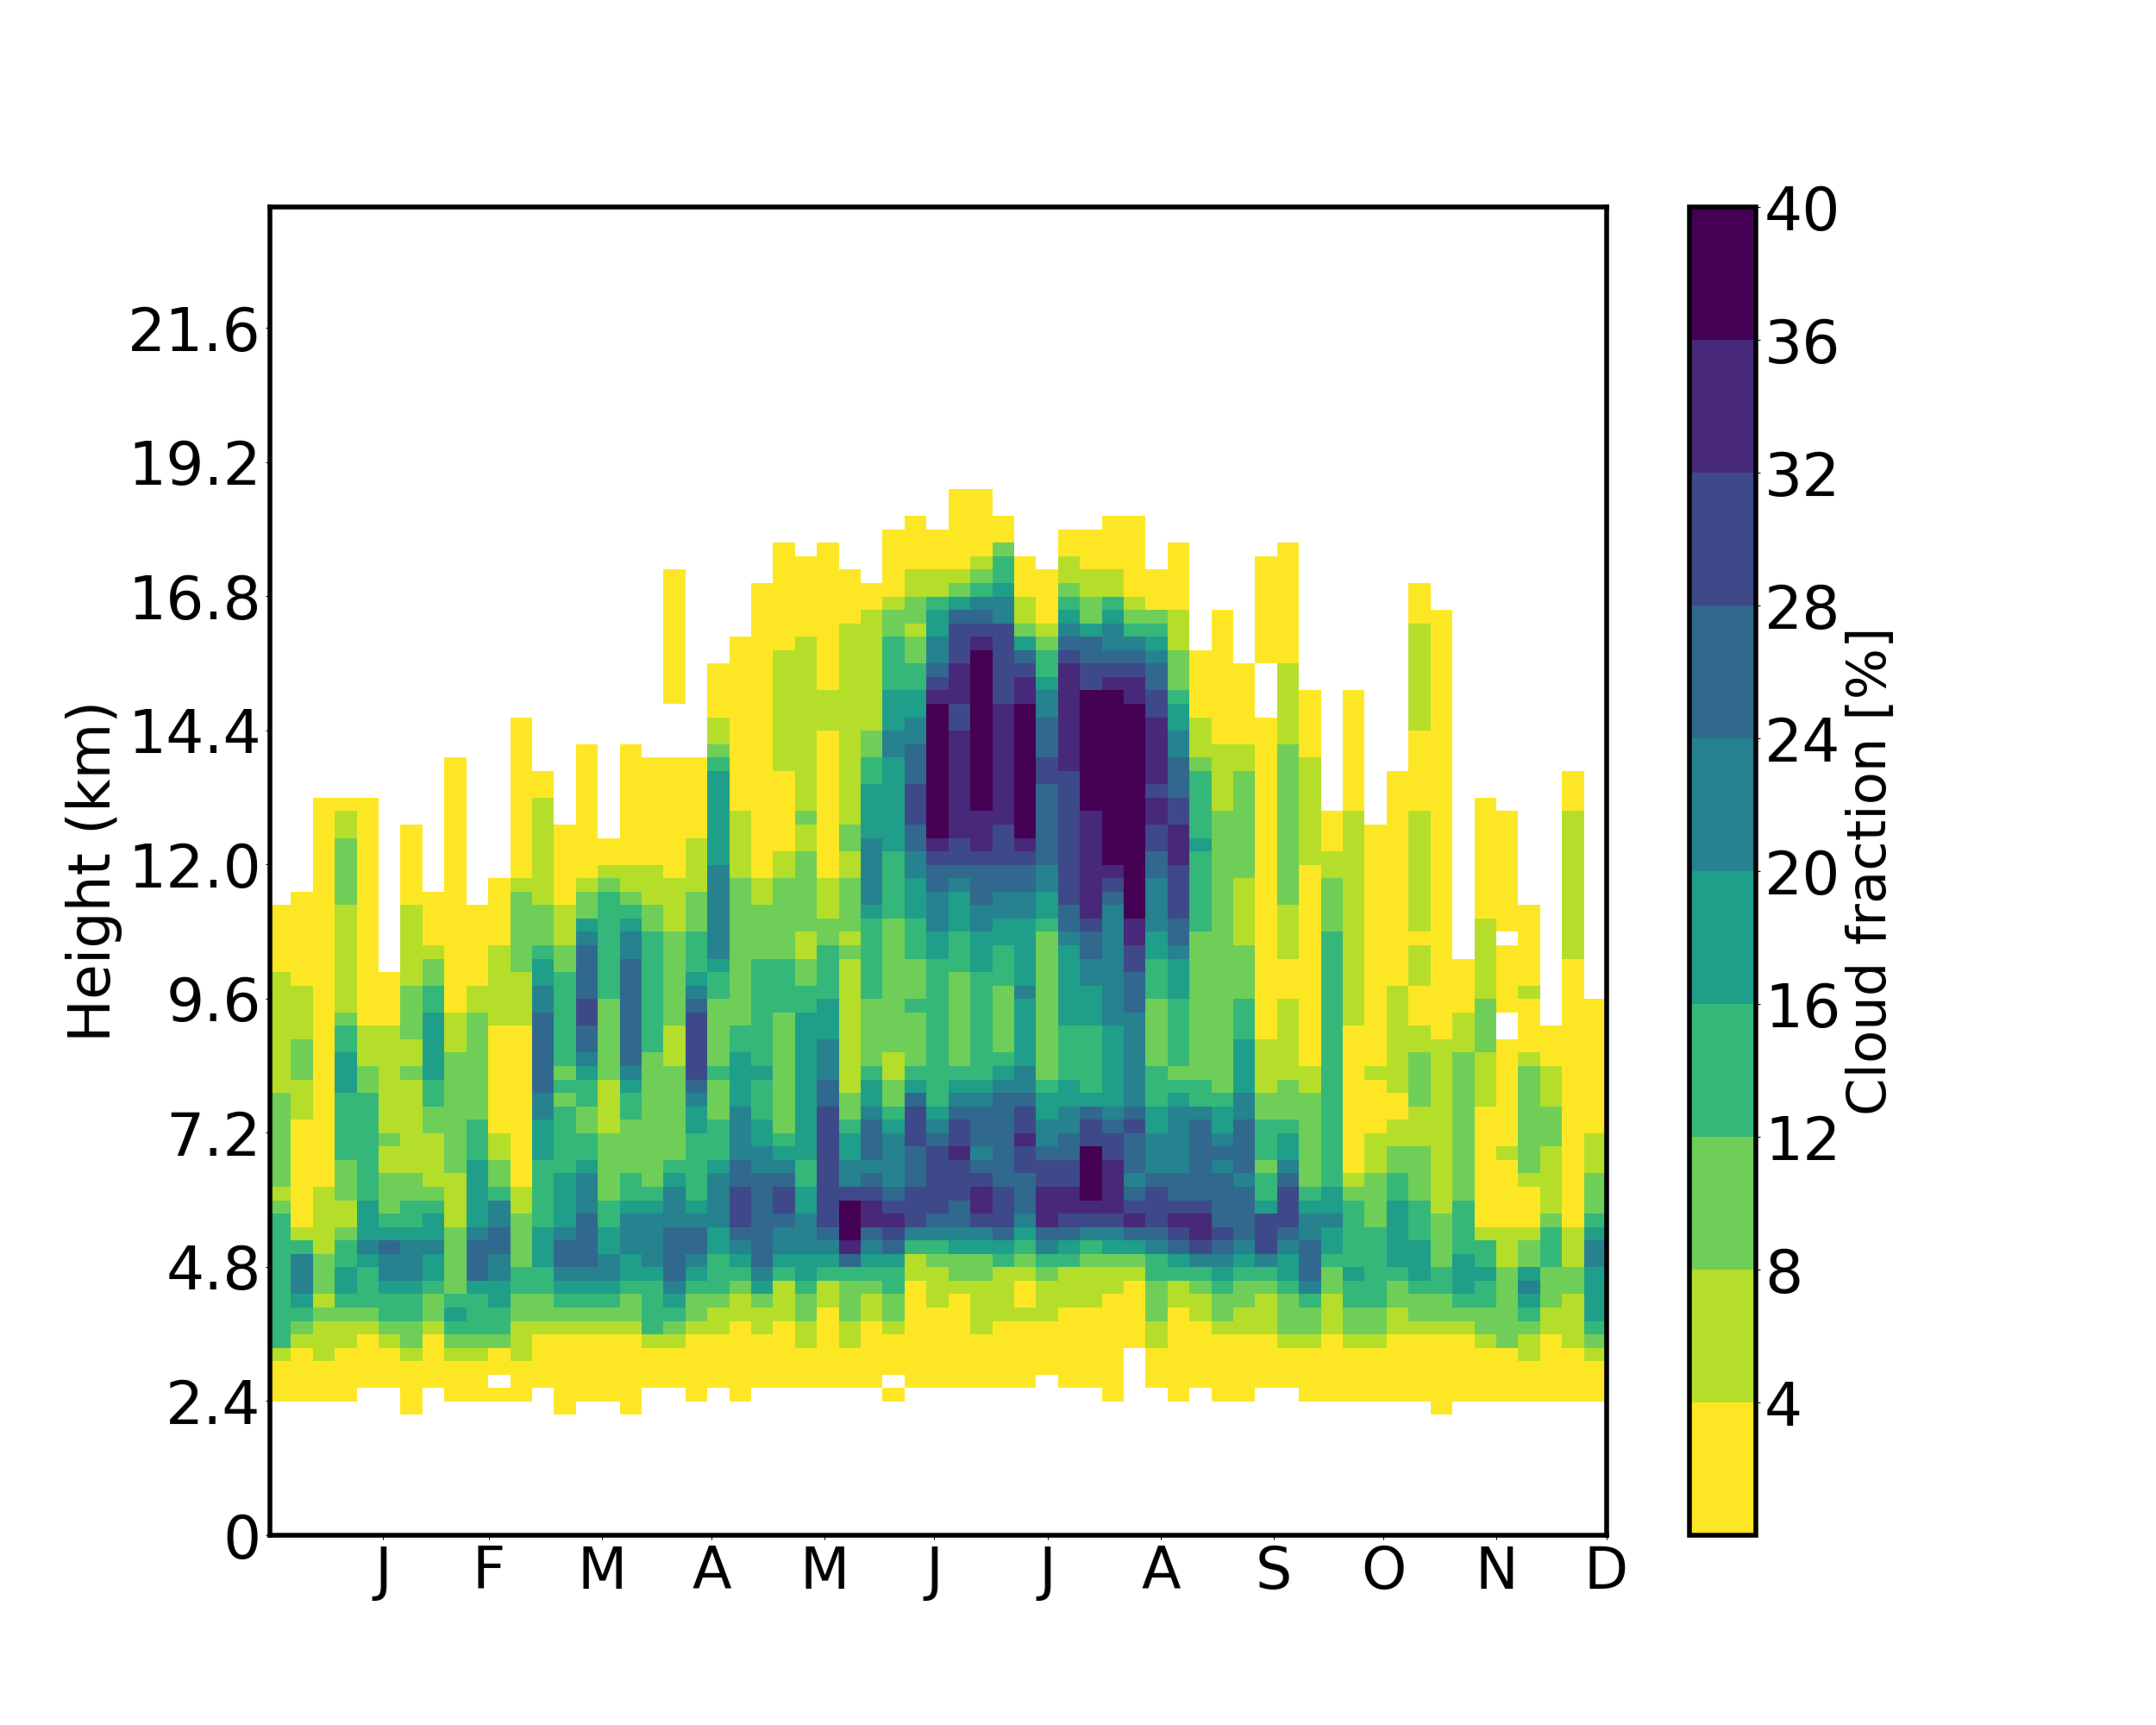
\includegraphics[width=\textwidth]{cloudsat_cloudfract_seasonal_monsoonmode_night.png}
        \label{fig:vertical_cloudfract4}

    \end{subfigure}
    
        \bigskip
        
   \begin{subfigure}[b]{0.5\textwidth}
       \centering
        \caption{westerly-dominated, daytime}       
        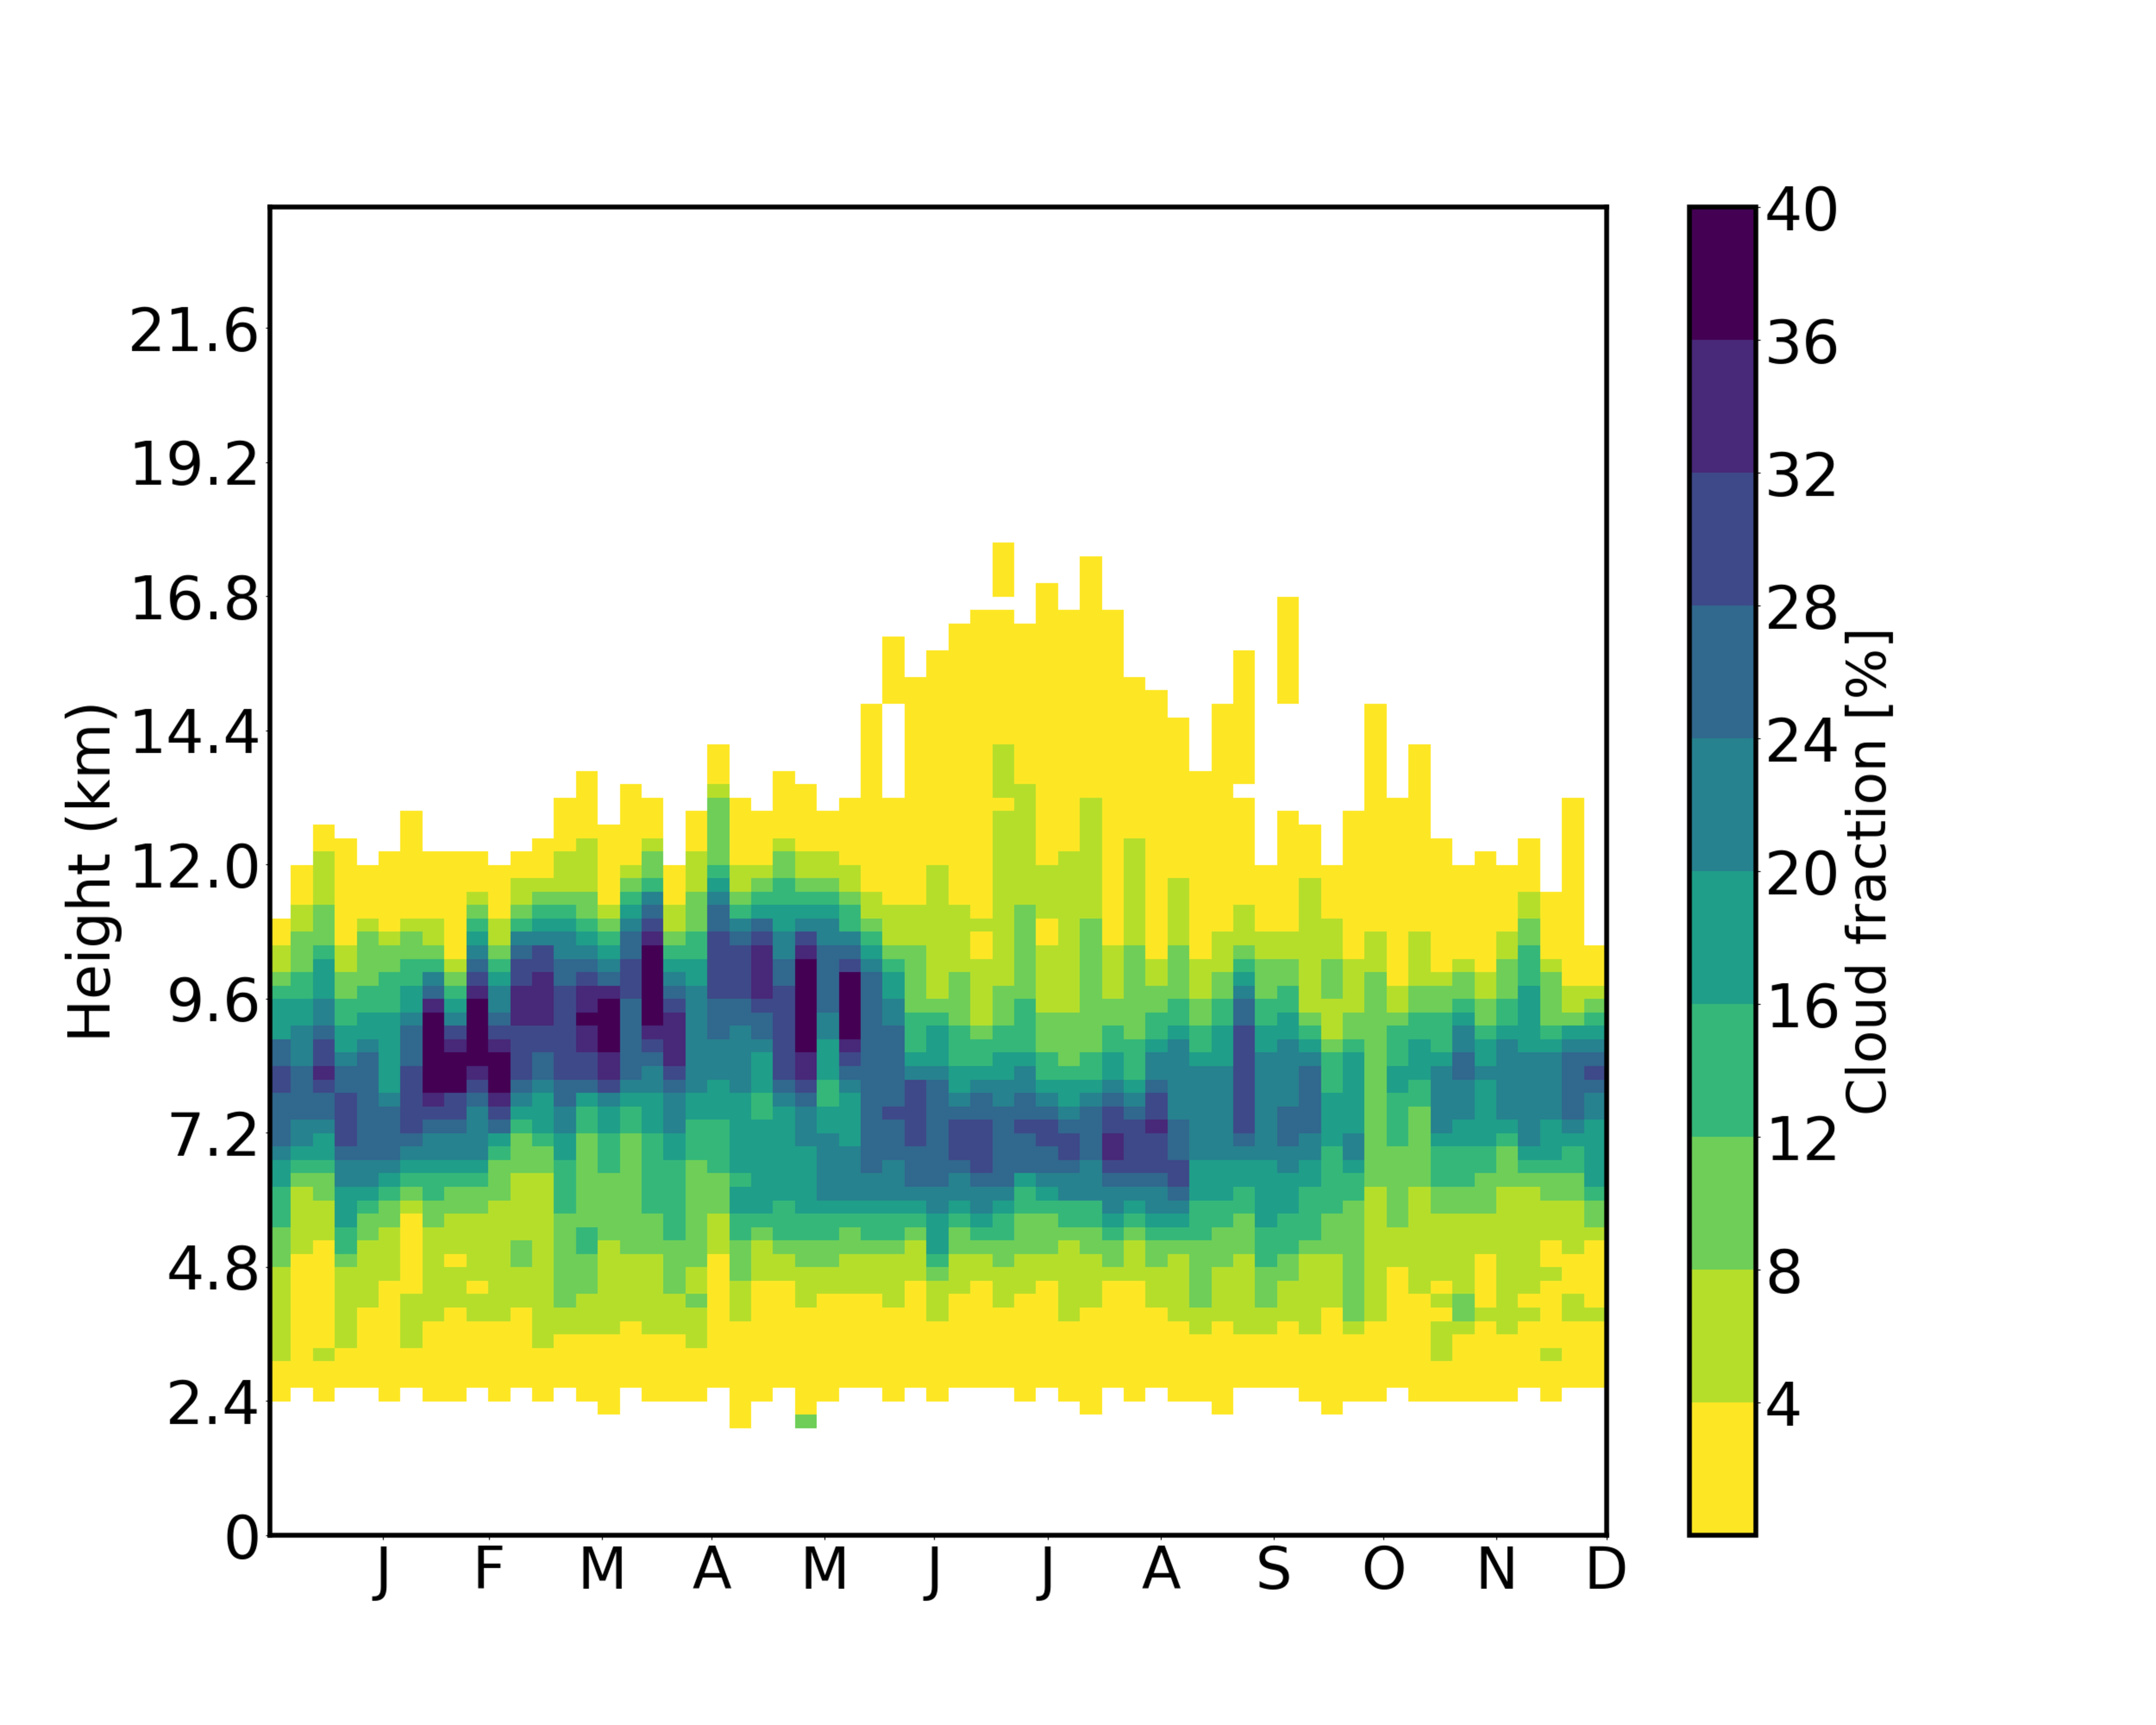
\includegraphics[width=\textwidth]{cloudsat_cloudfract_seasonal_westerlymode_day.png}
        \label{fig:vertical_cloudfract5}

    \end{subfigure}%
    ~ 
    \begin{subfigure}[b]{0.5\textwidth}
        \centering
\caption{westerly-dominated, nighttime}        
        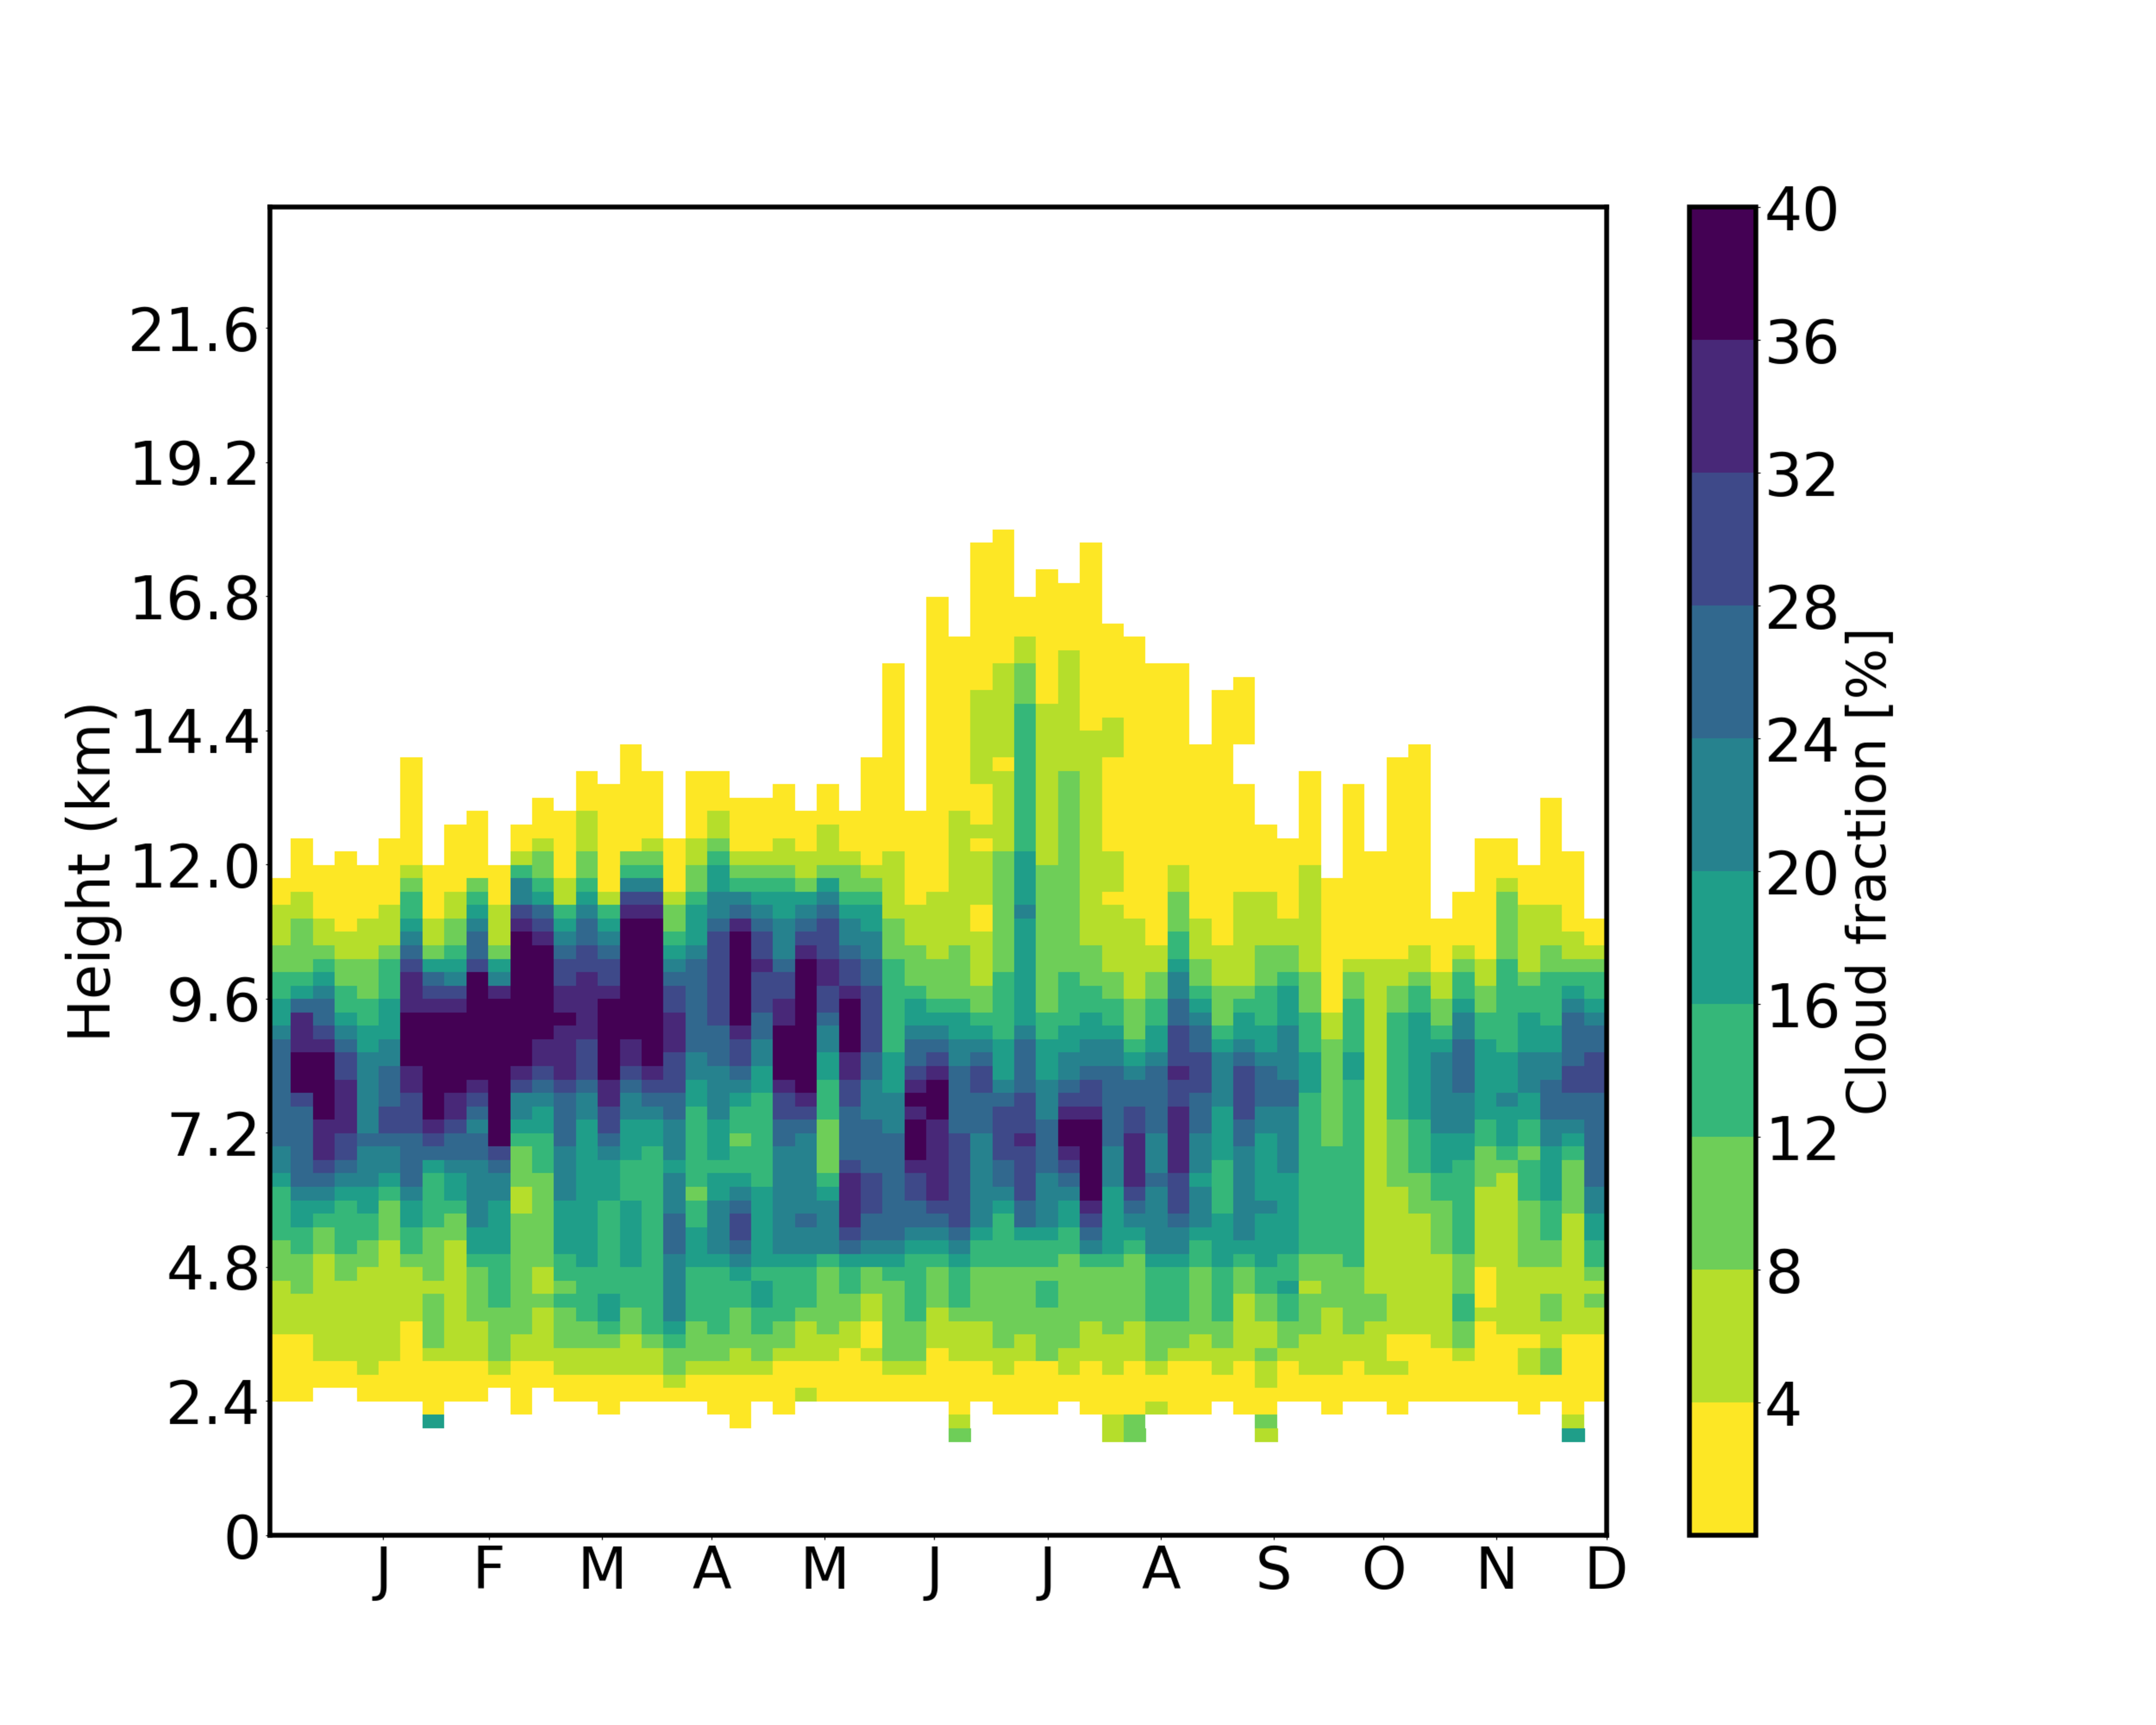
\includegraphics[width=\textwidth]{cloudsat_cloudfract_seasonal_westerlymode_night.png}
        \label{fig:vertical_cloudfract6}
    \end{subfigure}
    \label{fig:vertical_cloudfract}
    \end{figure}

\begin{figure}\ContinuedFloat
    \begin{subfigure}[b]{0.5\textwidth}
        \centering
        \caption{transition zone, daytime }        
        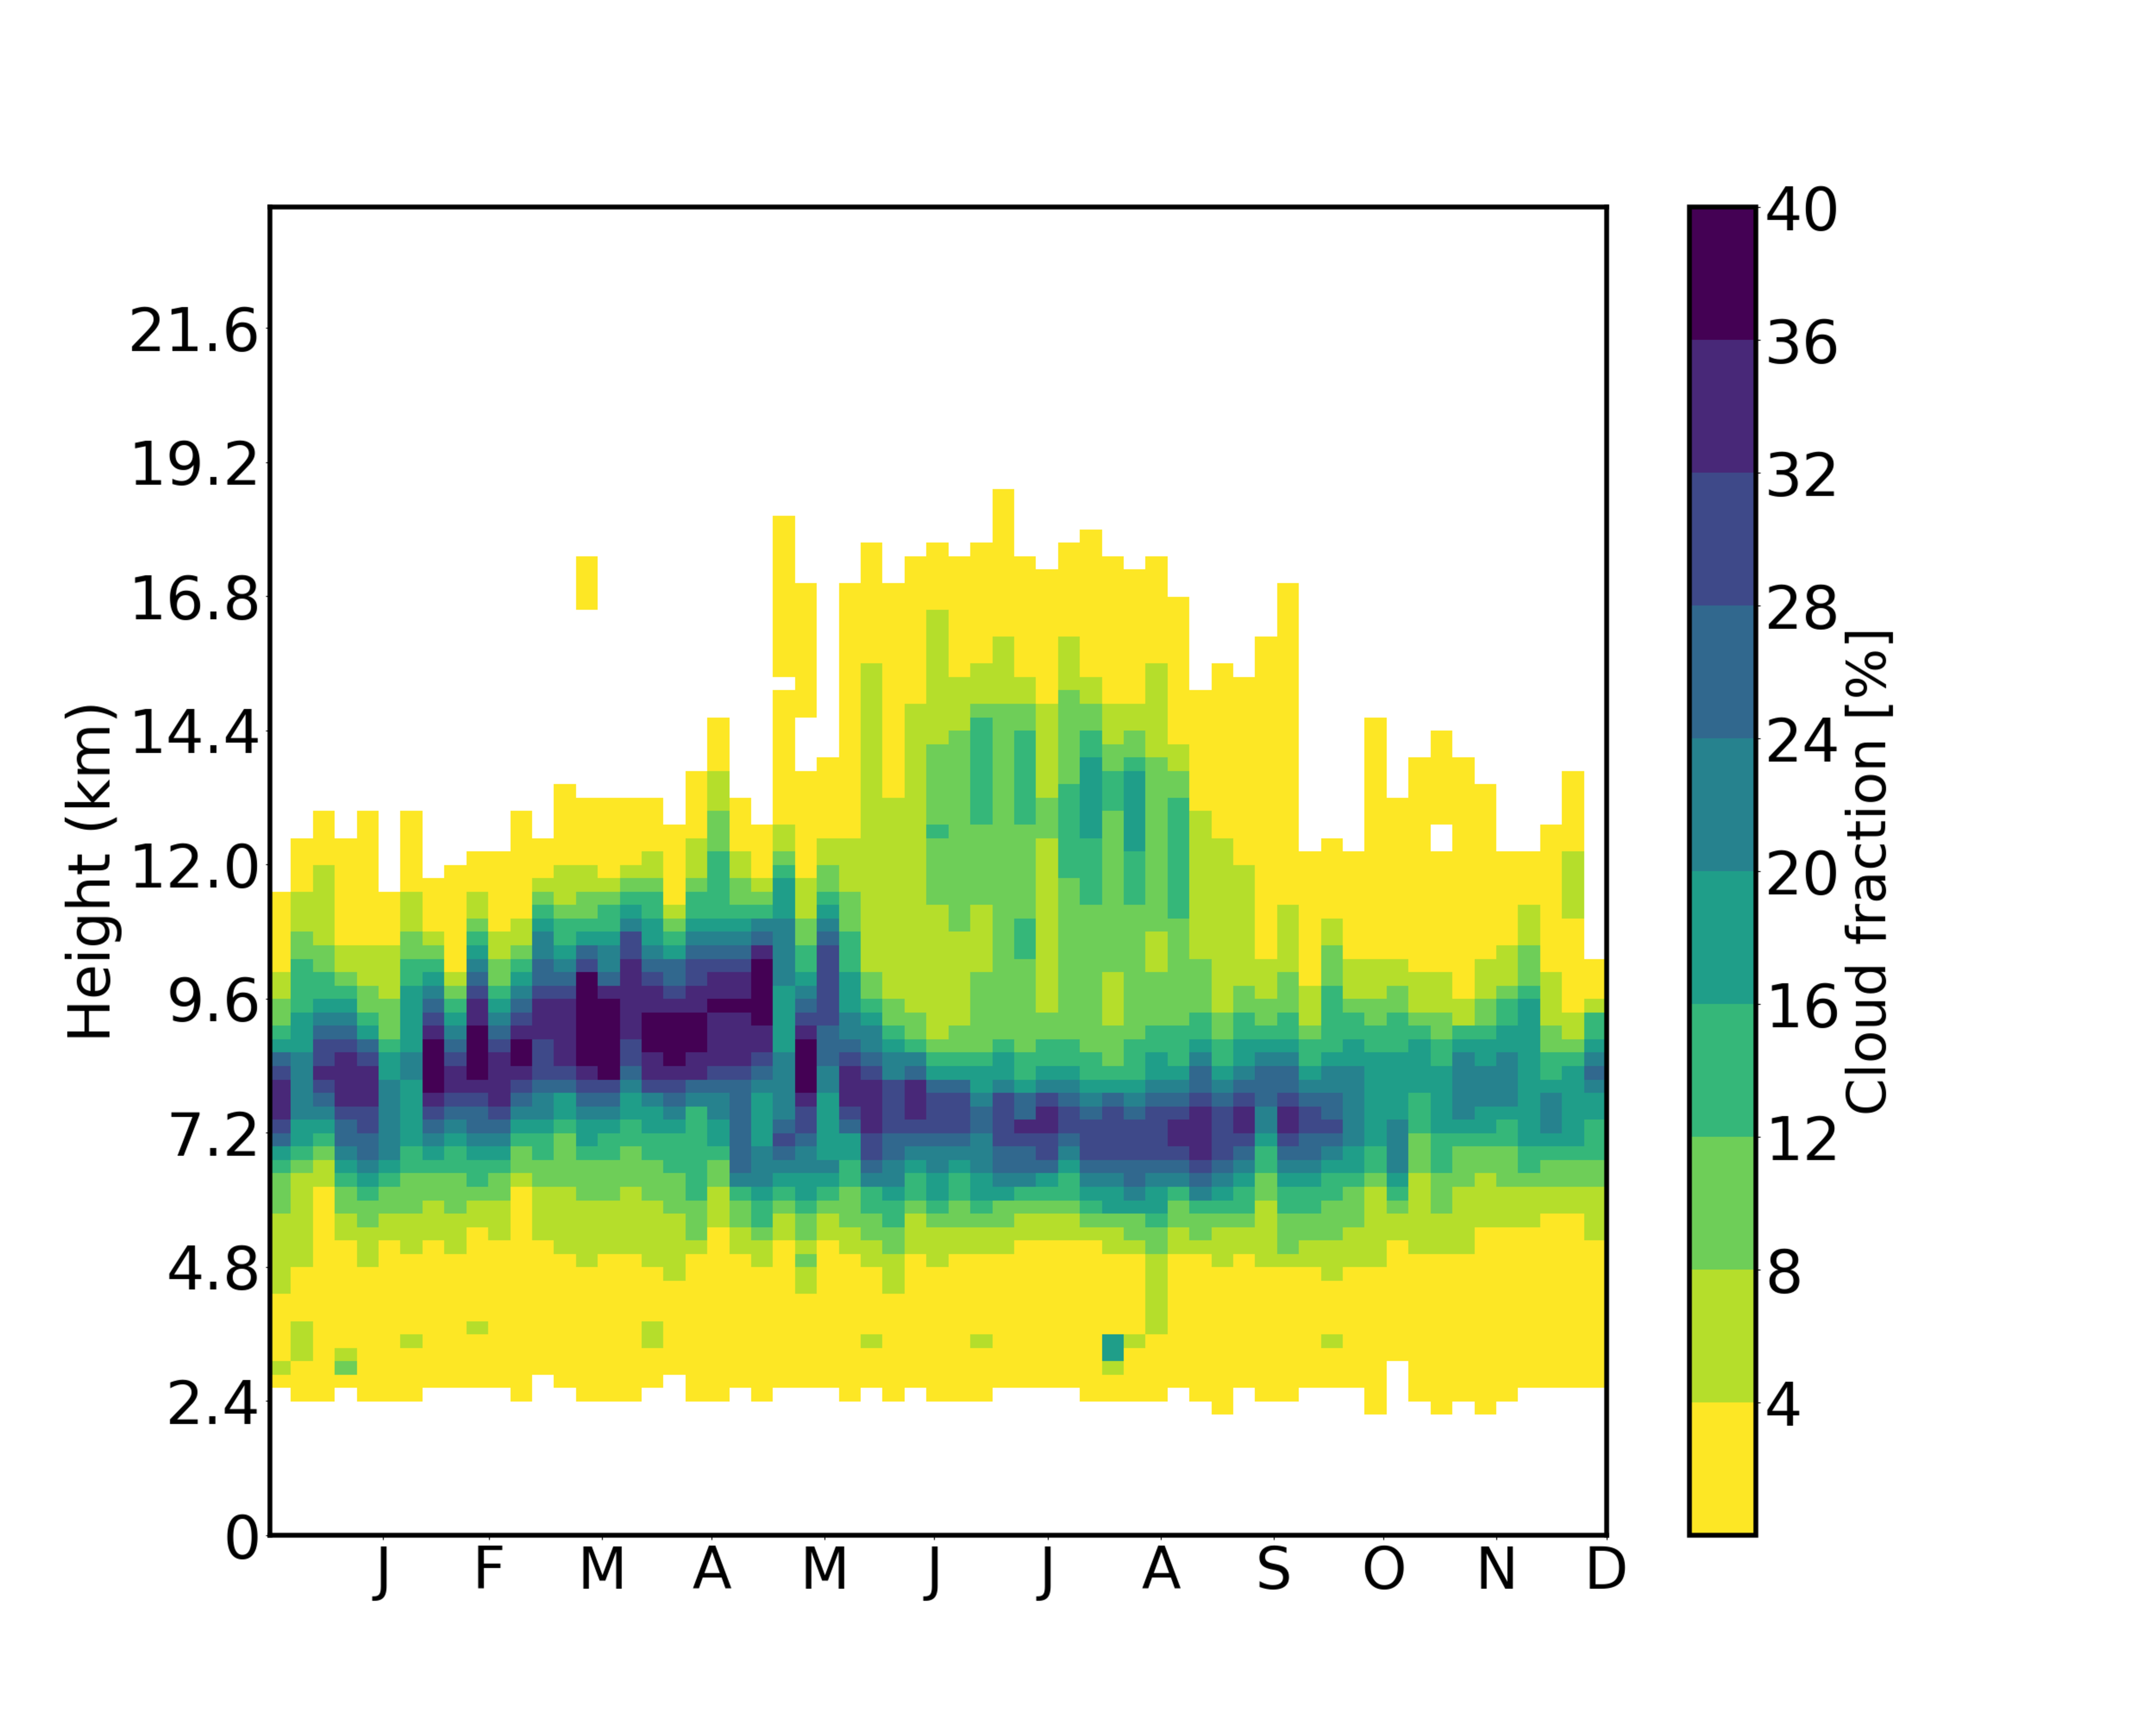
\includegraphics[width=\textwidth]{cloudsat_cloudfract_seasonal_transitionmode_day.png}
              \label{fig:vertical_cloudfract7}

    \end{subfigure}%
    ~ 
    \begin{subfigure}[b]{0.5\textwidth}
        \centering
        \caption{transition zone, nighttime }        
        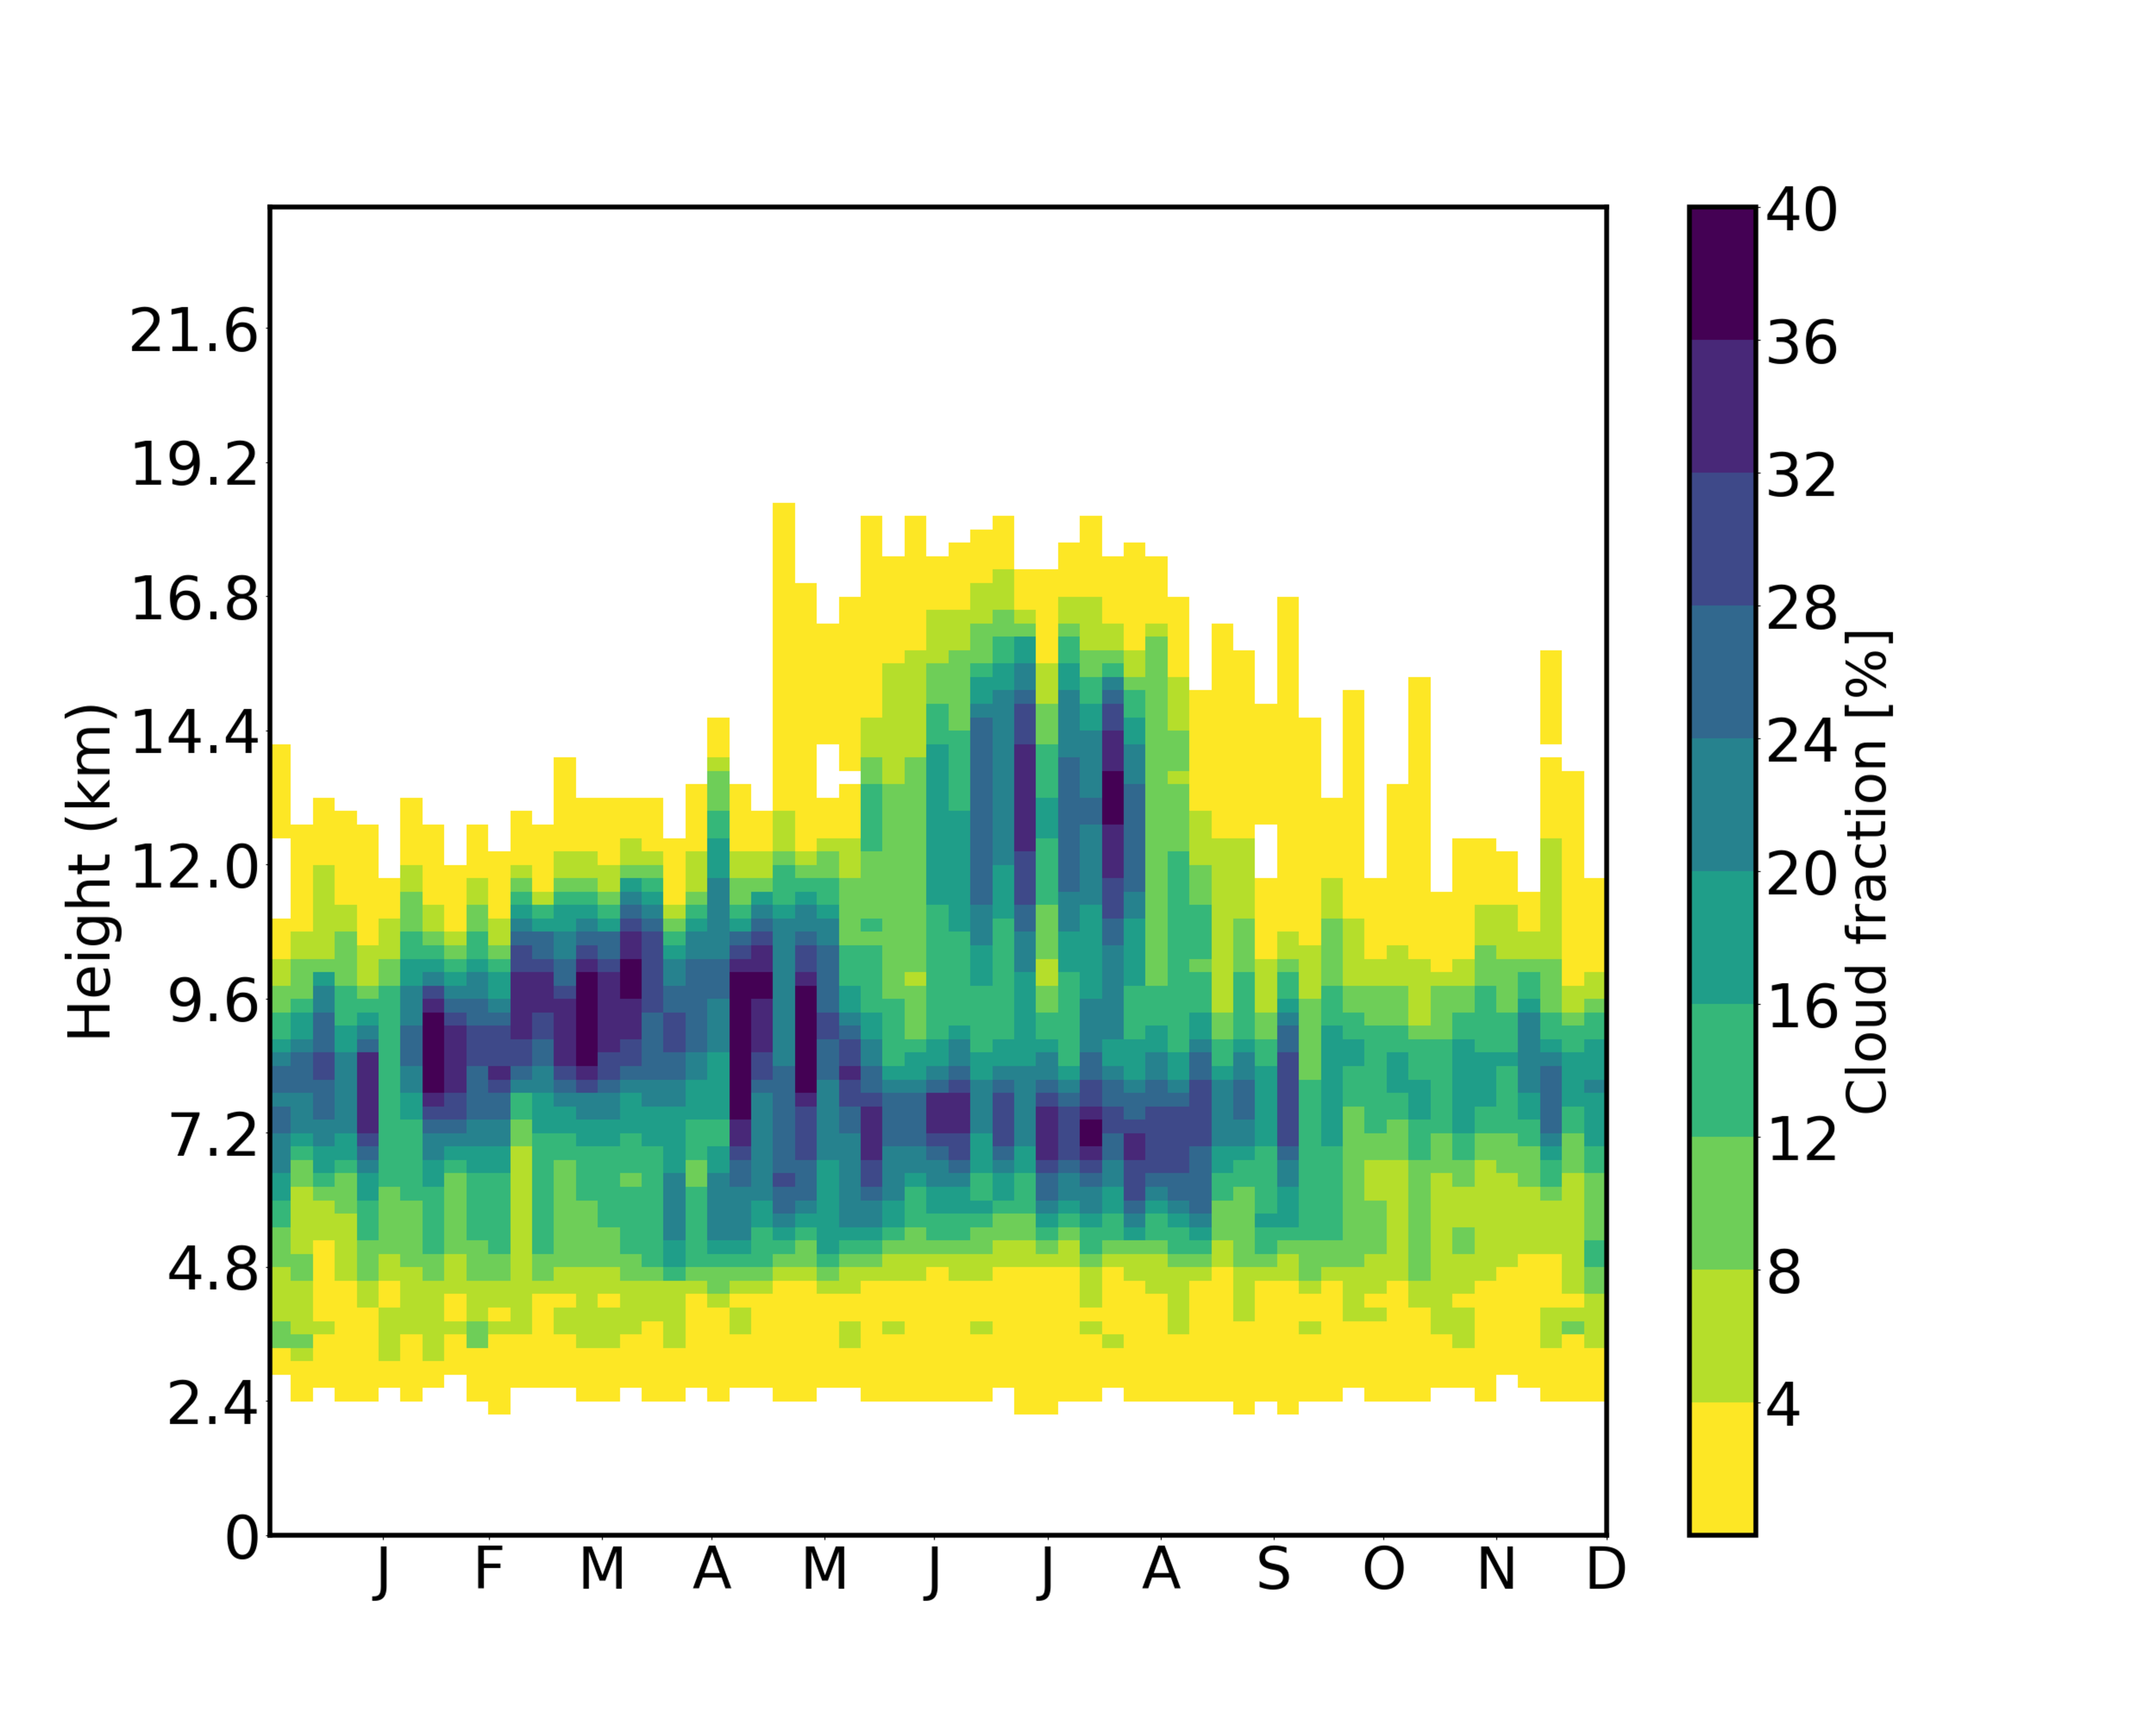
\includegraphics[width=\textwidth]{cloudsat_cloudfract_seasonal_transitionmode_night.png}
              \label{fig:vertical_cloudfract8}
        \end{subfigure}   
    \caption{Monthly variation of vertical cloud fractions (\%) for the TP domain (a -- b), monsoon-dominated domain (c -- d), westerly-dominated domain (e --f) and transition zone (g -- h) during daytime compared nighttime as derived from 2B-GEOPROF and 2B-GEOPROF-LIDAR (2006 -- 2011). Cloud fractions include CPR and CALIOP detections and are presented as a 6-day average for each vertical profile bin (0.24 km).}   
\label{fig:vertical_cloudfract}
\end{figure}

In addition to cloud fractions at different heights, we examined the normalized contoured-frequency-by-altitude diagram (CFAD) of radar reflectivities as derived from 2B-GEOPROF (2006 -- 2011). The CFAD presents the number of occurrences in each height-reflectivity bin in relation to the total number of values in the cloudy profiles \citep{CFAD1995} and reveals thereby frequencies of particle sizes for different cloud altitudes (Fig. \ref{fig:CFAD}). Both the seasonality of cloud characteristics as well as the regional dependence are well reflected in the radar reflectivity profiles: the two most distinct CFAD are the monsoon-dominated domain between May and September (Fig. \ref{fig:CFAD3}) compared to the westerly-dominated domain between October and April (Fig. \ref{fig:CFAD6}). In general, differences between the westerly and monsoon season outweigh regional and day-night differences (not shown here), since both seasons entail two distinct radar reflectivity profiles which dominate the pattern in the TP domain as well as in each of the three subregions (Fig. \ref{fig:CFAD}). The frequency values between -25 and -5 dBZ from 5 to 10 km a.s.l. increase significantly during the westerly season, resulting in a triangle-shaped CFAD (Fig. \ref{fig:CFAD2}, \ref{fig:CFAD4}, \ref{fig:CFAD6}, \ref{fig:CFAD8}). The largest reflectivities during the westerly season occur below 7 km a.s.l., whereas lower reflectivity values which indicate smaller hydrometeors, are most frequent between 7 and 10 km a.s.l.. All CFAD of the westerly season exhibit the highest frequencies for negative radar reflectivities and values above 10 dBZ are generally less frequent compared to the monsoon season. This reflects the drier westerly season (see also Fig. \ref{fig:cloud_occ}), since precipitation is generally associated with higher radar reflectivity values. Meanwhile, frequency values in the monsoon season tend to be more spread over the height-reflectivity space, suggesting a higher variation of particle sizes occurring at different levels (Fig. \ref{fig:CFAD1}, \ref{fig:CFAD3}, \ref{fig:CFAD5}, \ref{fig:CFAD7}). This is consistent with the vertical cloud fractions and cloud types (Fig. \ref{fig:vertical_cloudfract}, \ref{fig:cld_type}), which exhibited higher variations for the monsoon compared to the westerly season. 



\begin{figure}[!htbp]
    \begin{subfigure}[b]{0.5\textwidth}
       \centering
        \caption{TP,   May -- Sep}
        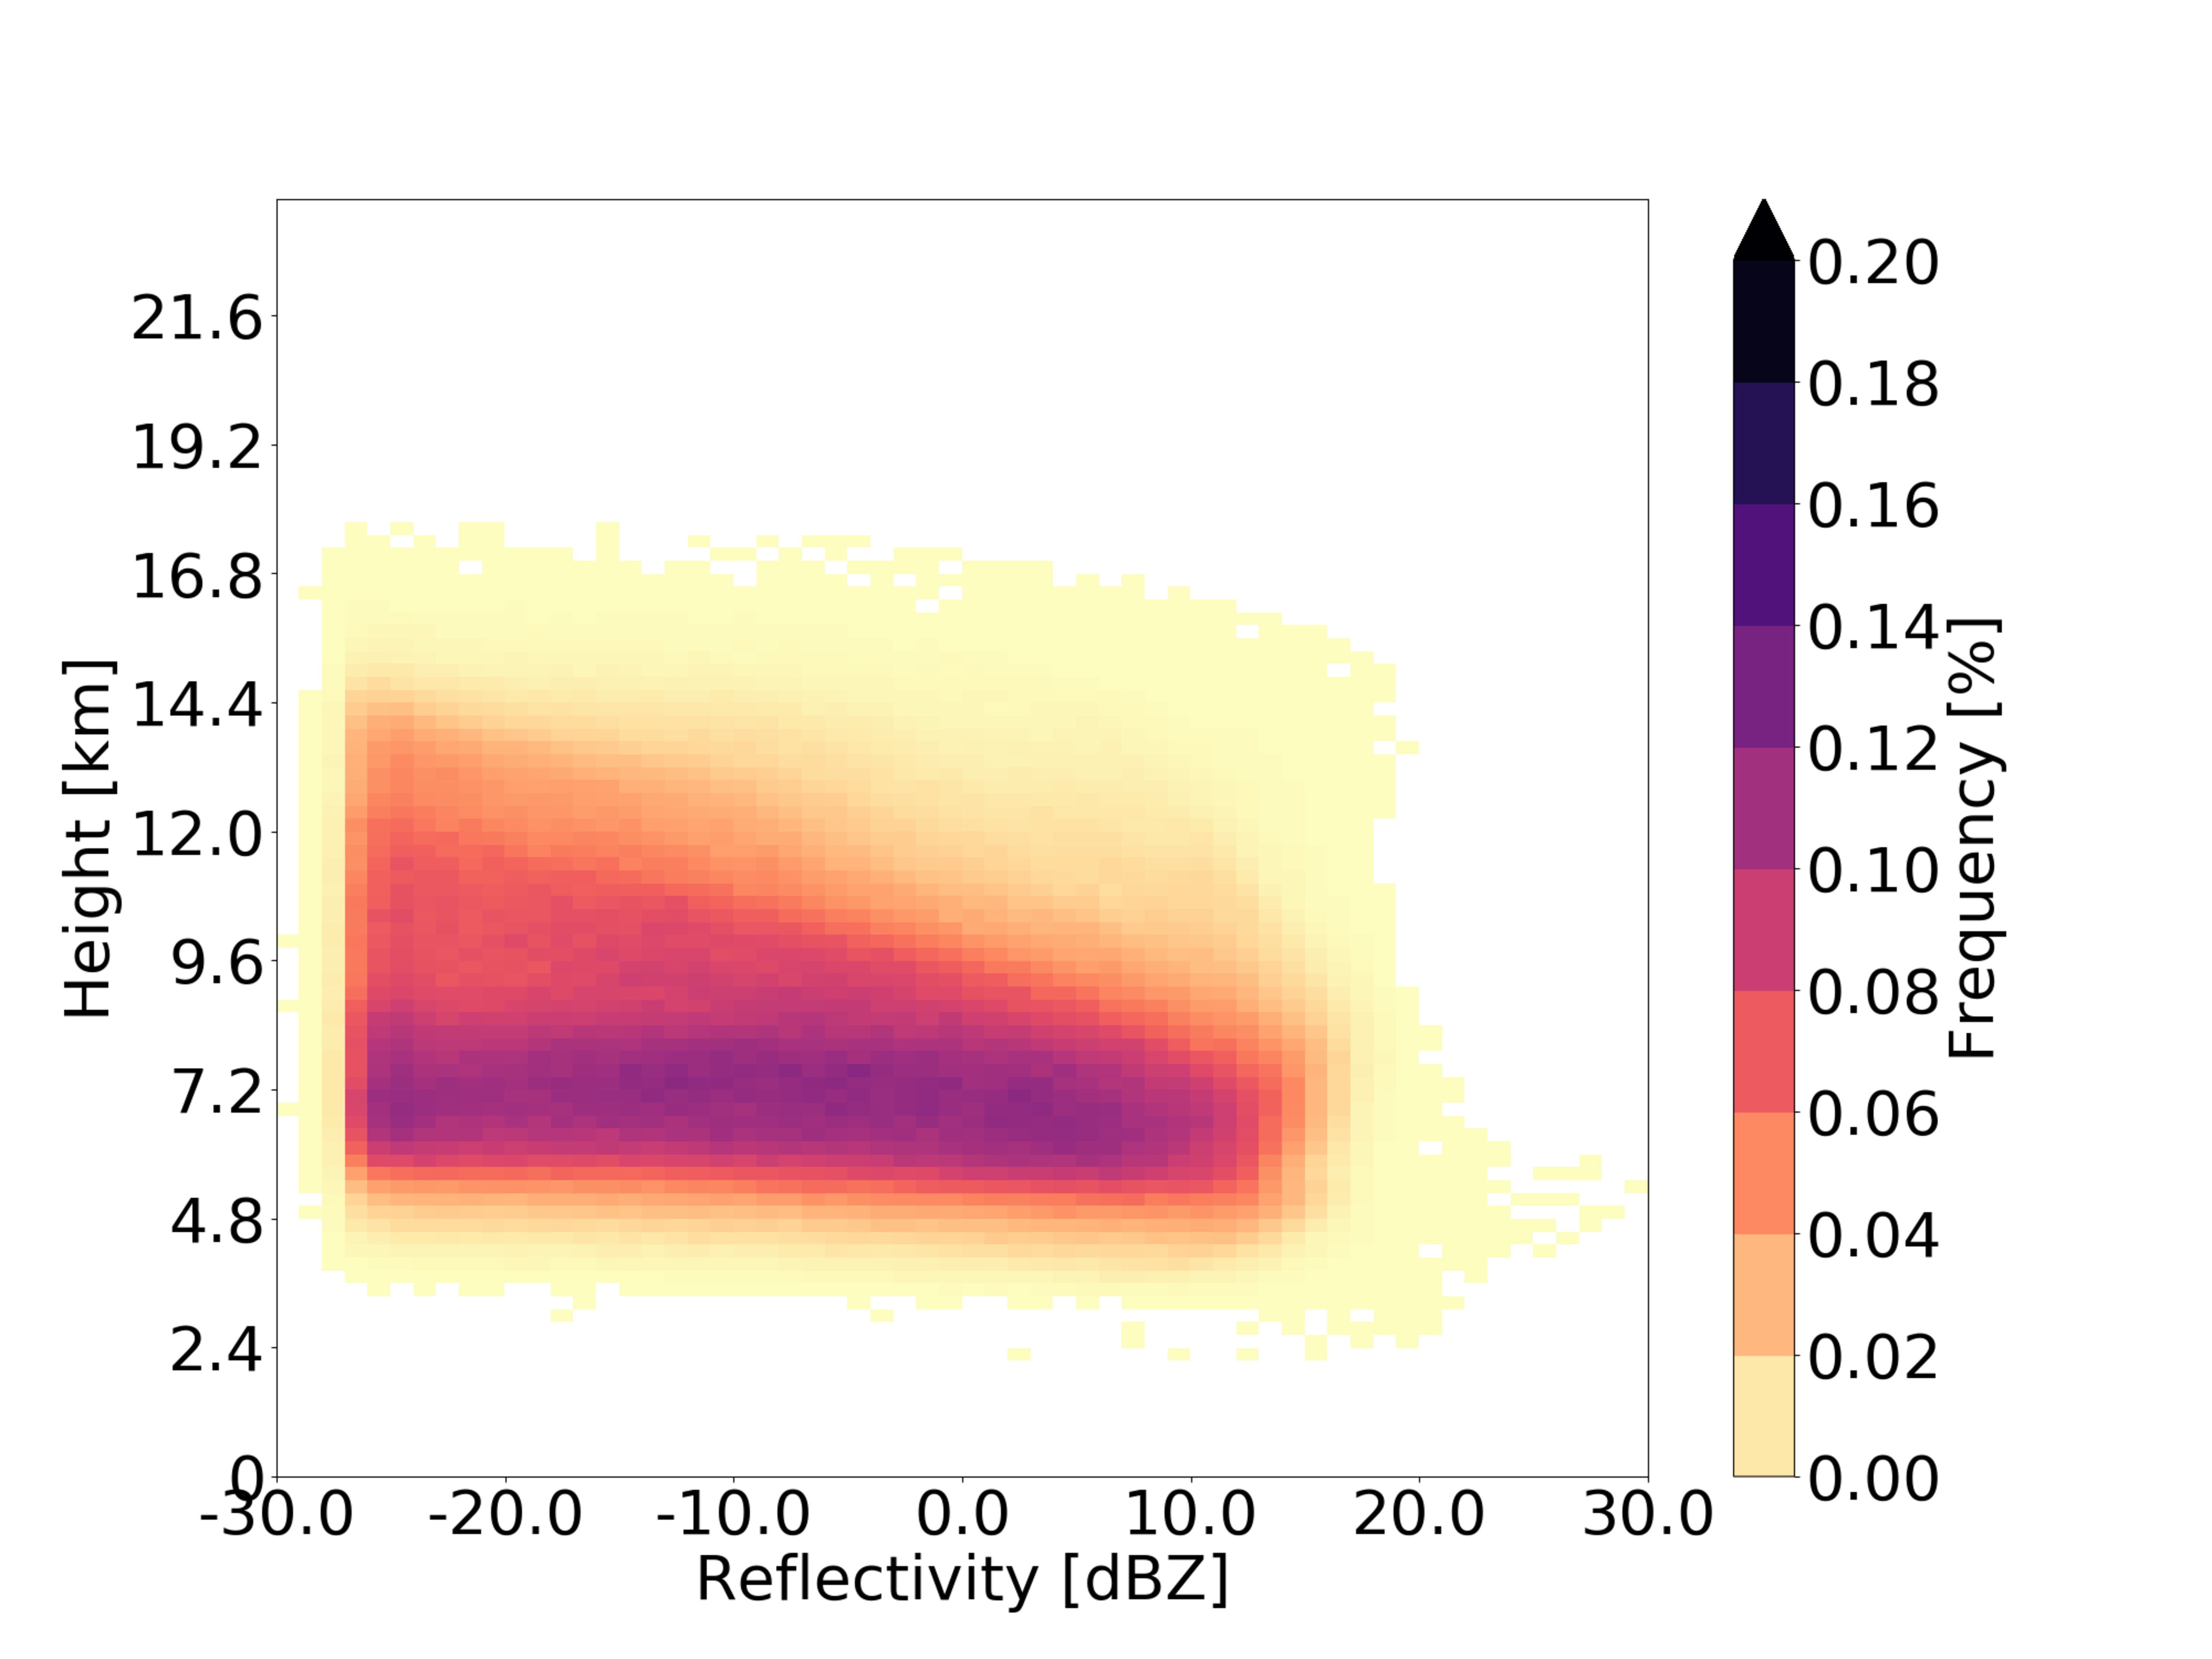
\includegraphics[width=\textwidth]{radar_reflect_TP_monsoonseason.png}
        \label{fig:CFAD1}

    \end{subfigure}%
    ~ 
    \begin{subfigure}[b]{0.5\textwidth}
        \centering
        \caption{TP,  Oct -- Apr }        
        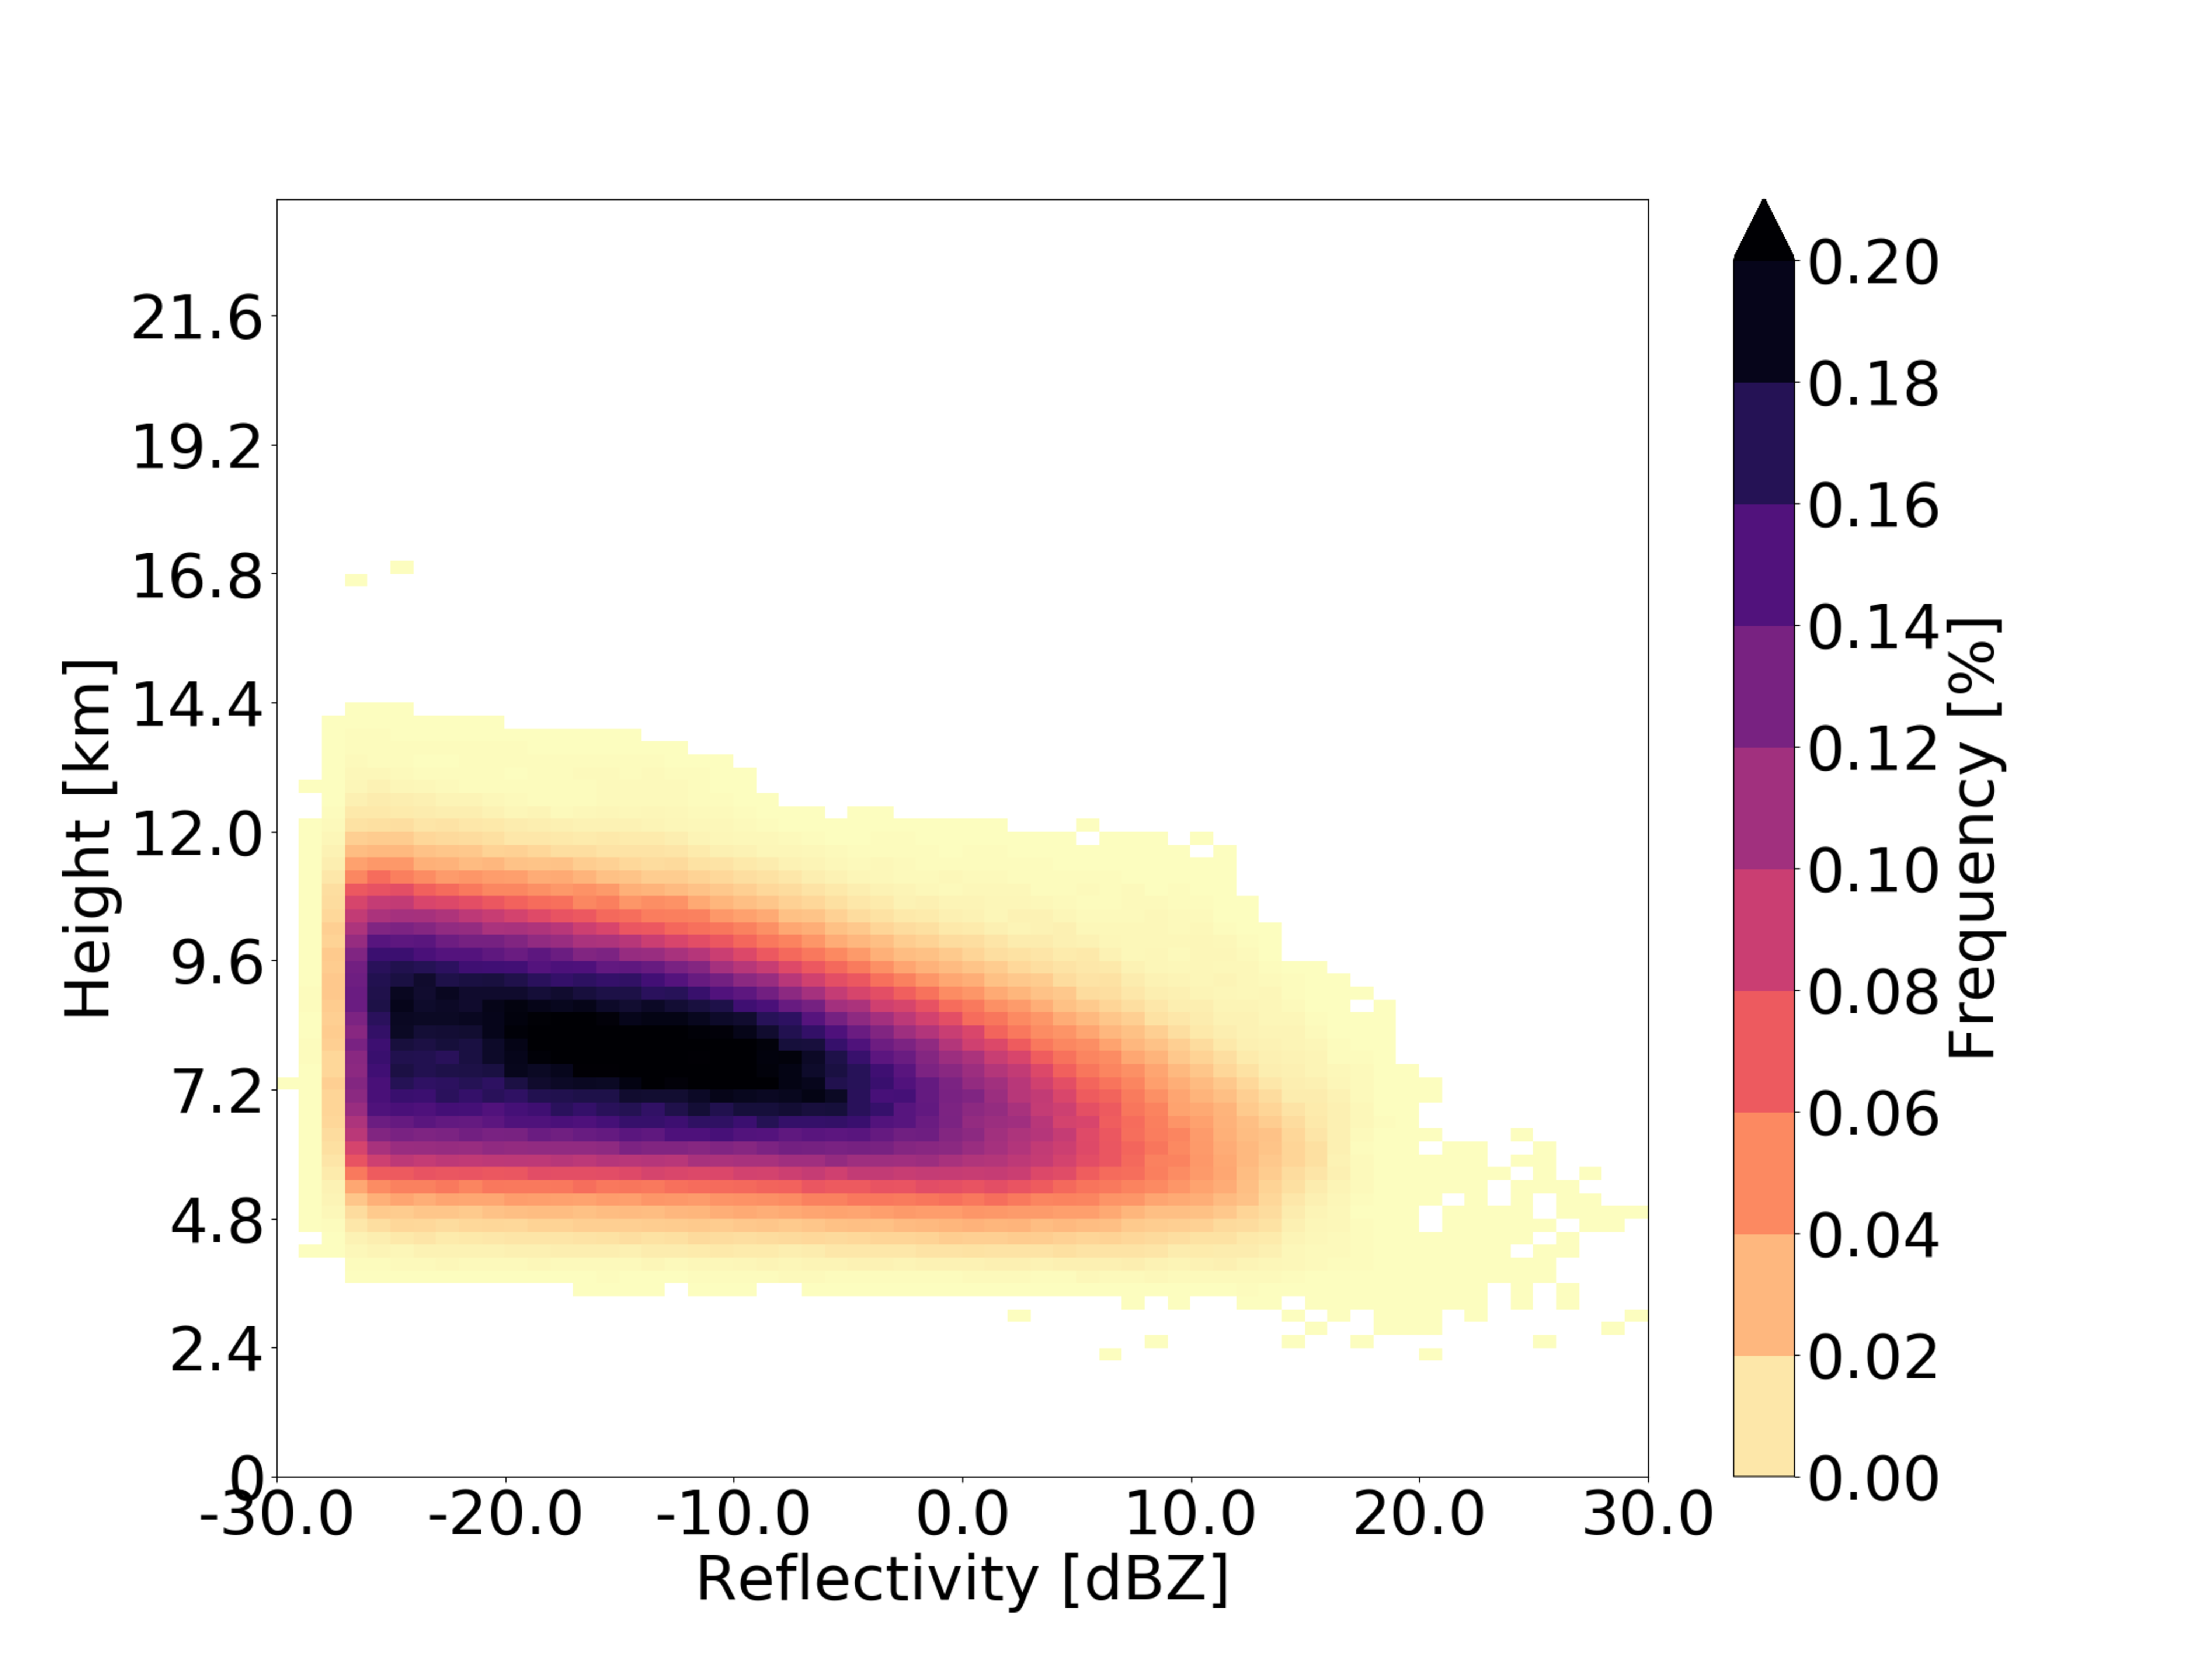
\includegraphics[width=\textwidth]{radar_reflect_TP_westerlyseason.png}
        \label{fig:CFAD2}
\end{subfigure}

    \begin{subfigure}[b]{0.5\textwidth}
       \centering
        \caption{monsoon-dominated, May -- Sep}
        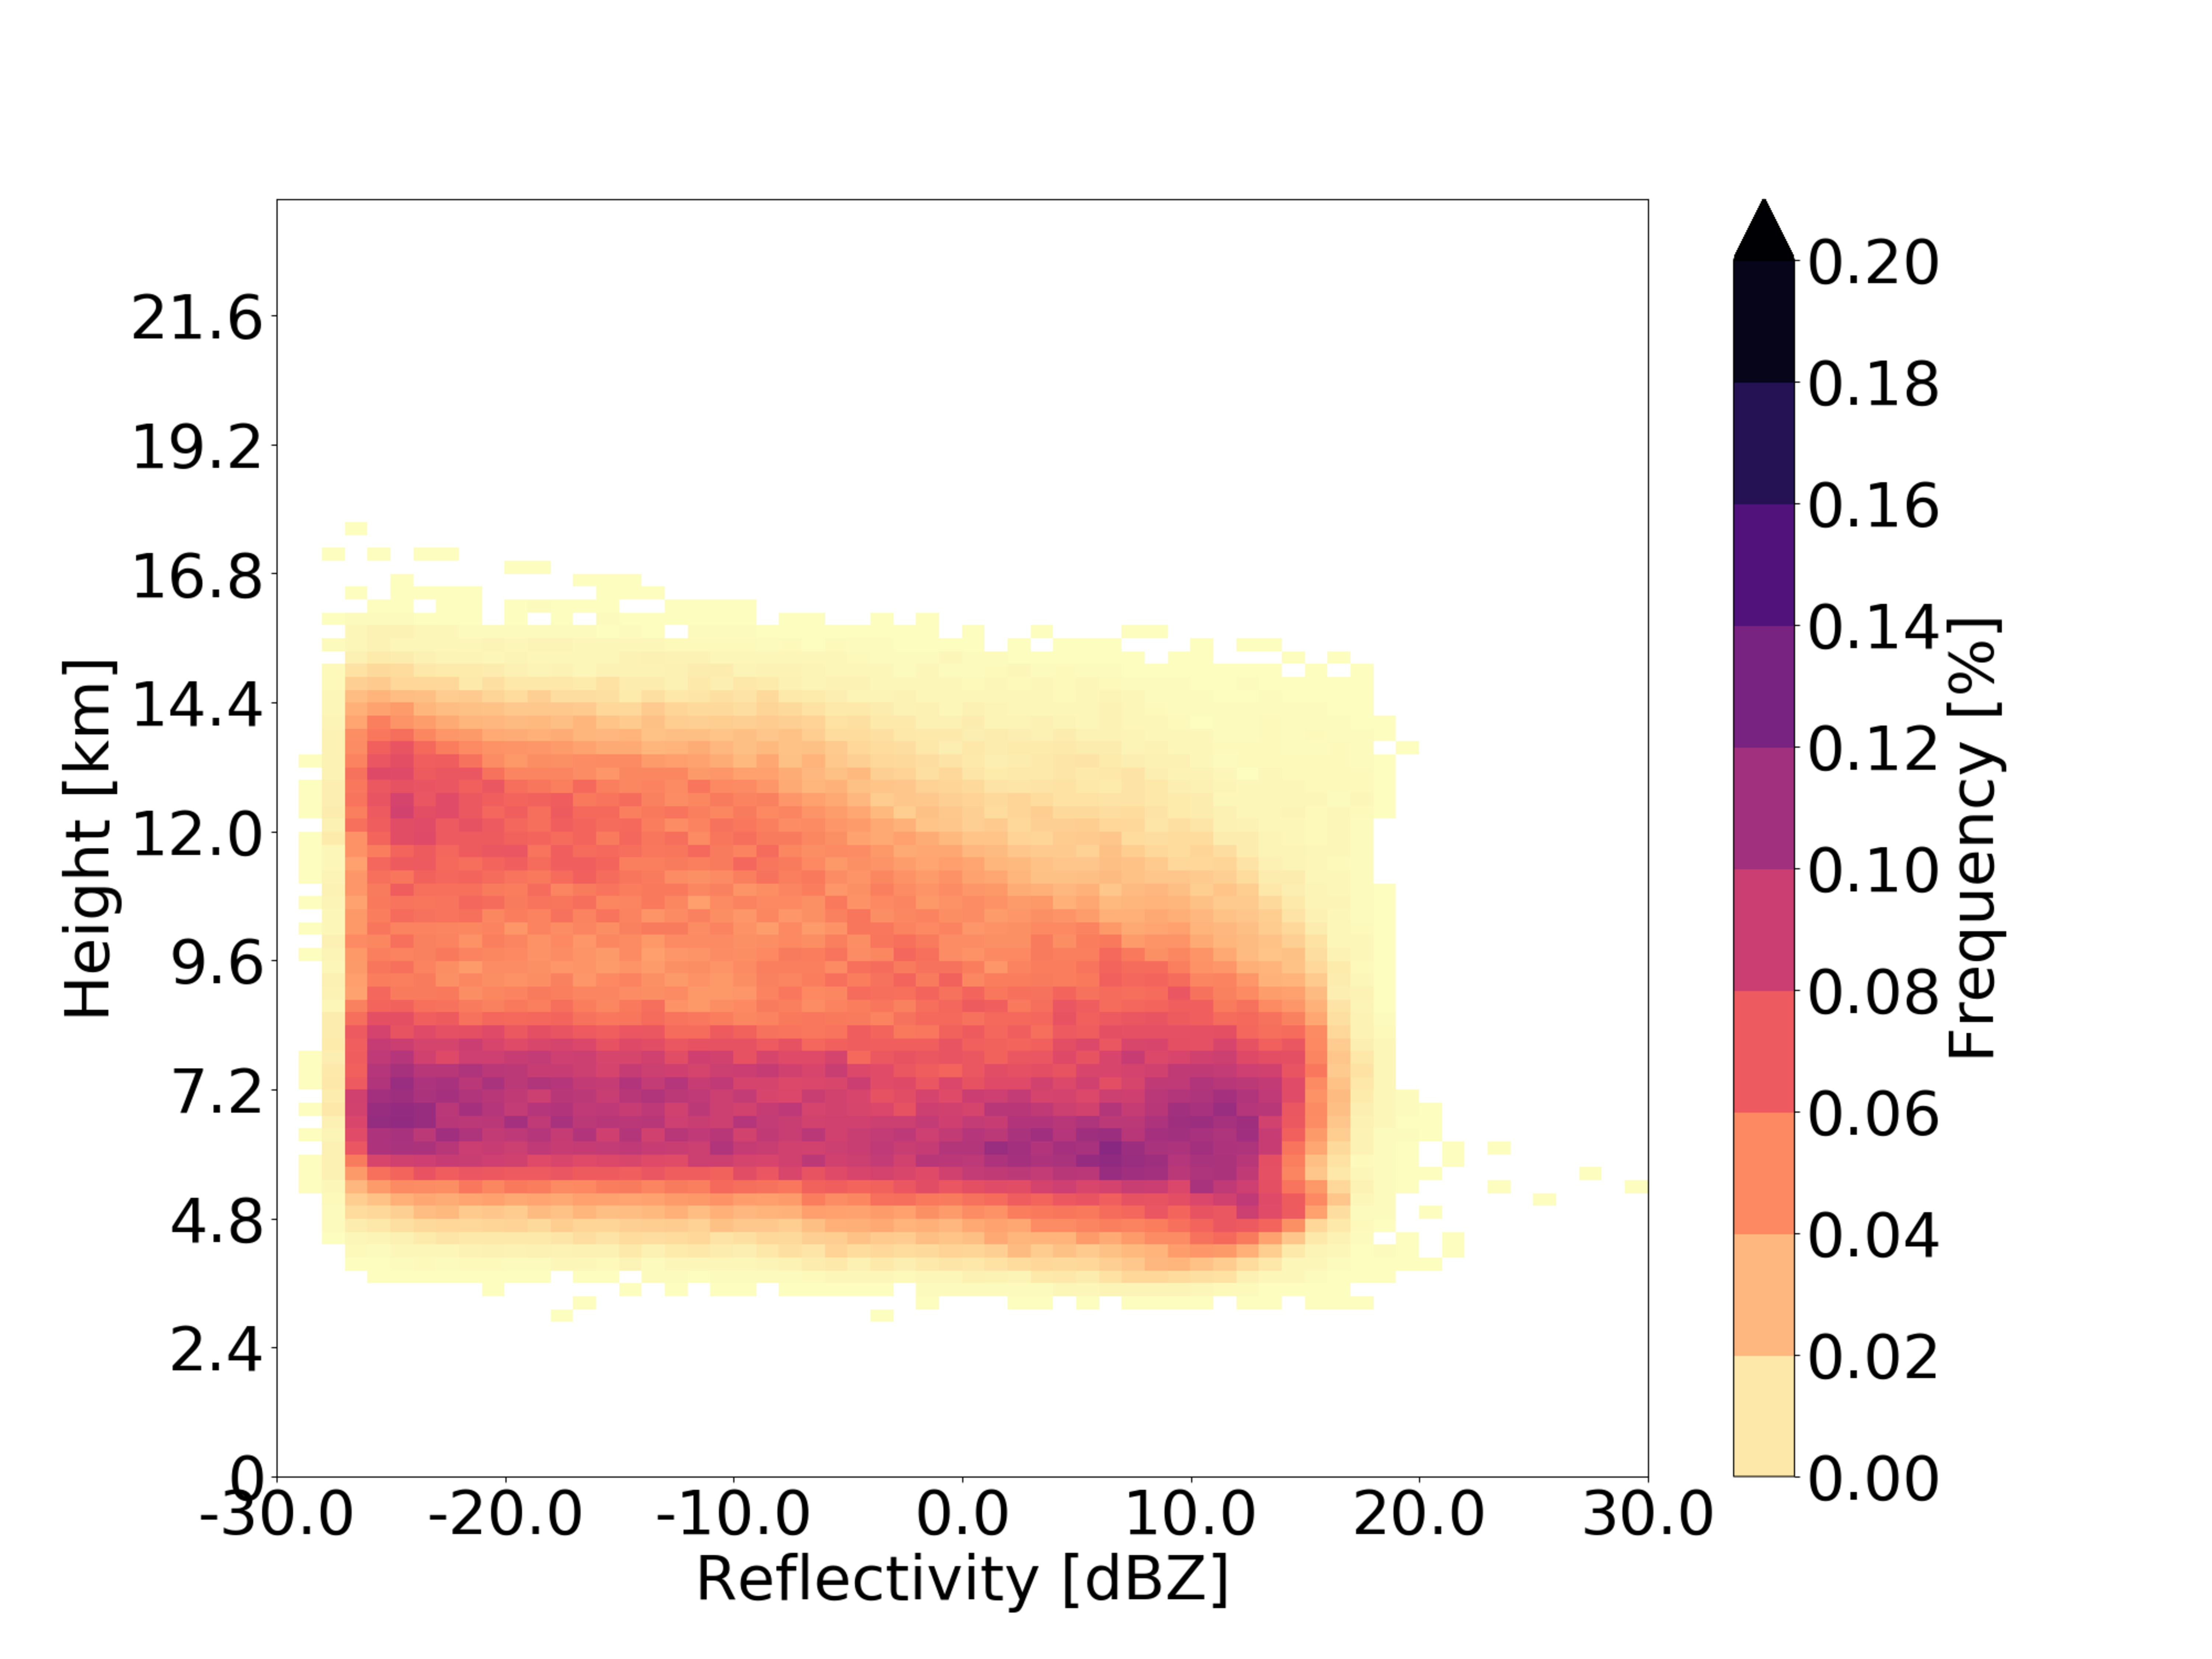
\includegraphics[width=\textwidth]{radar_reflect_monsoondomain_monsoonseason.png}
\label{fig:CFAD3}
    \end{subfigure}%
    ~ 
    \begin{subfigure}[b]{0.5\textwidth}
        \centering
        \caption{monsoon-dominated, Oct -- Apr }        
        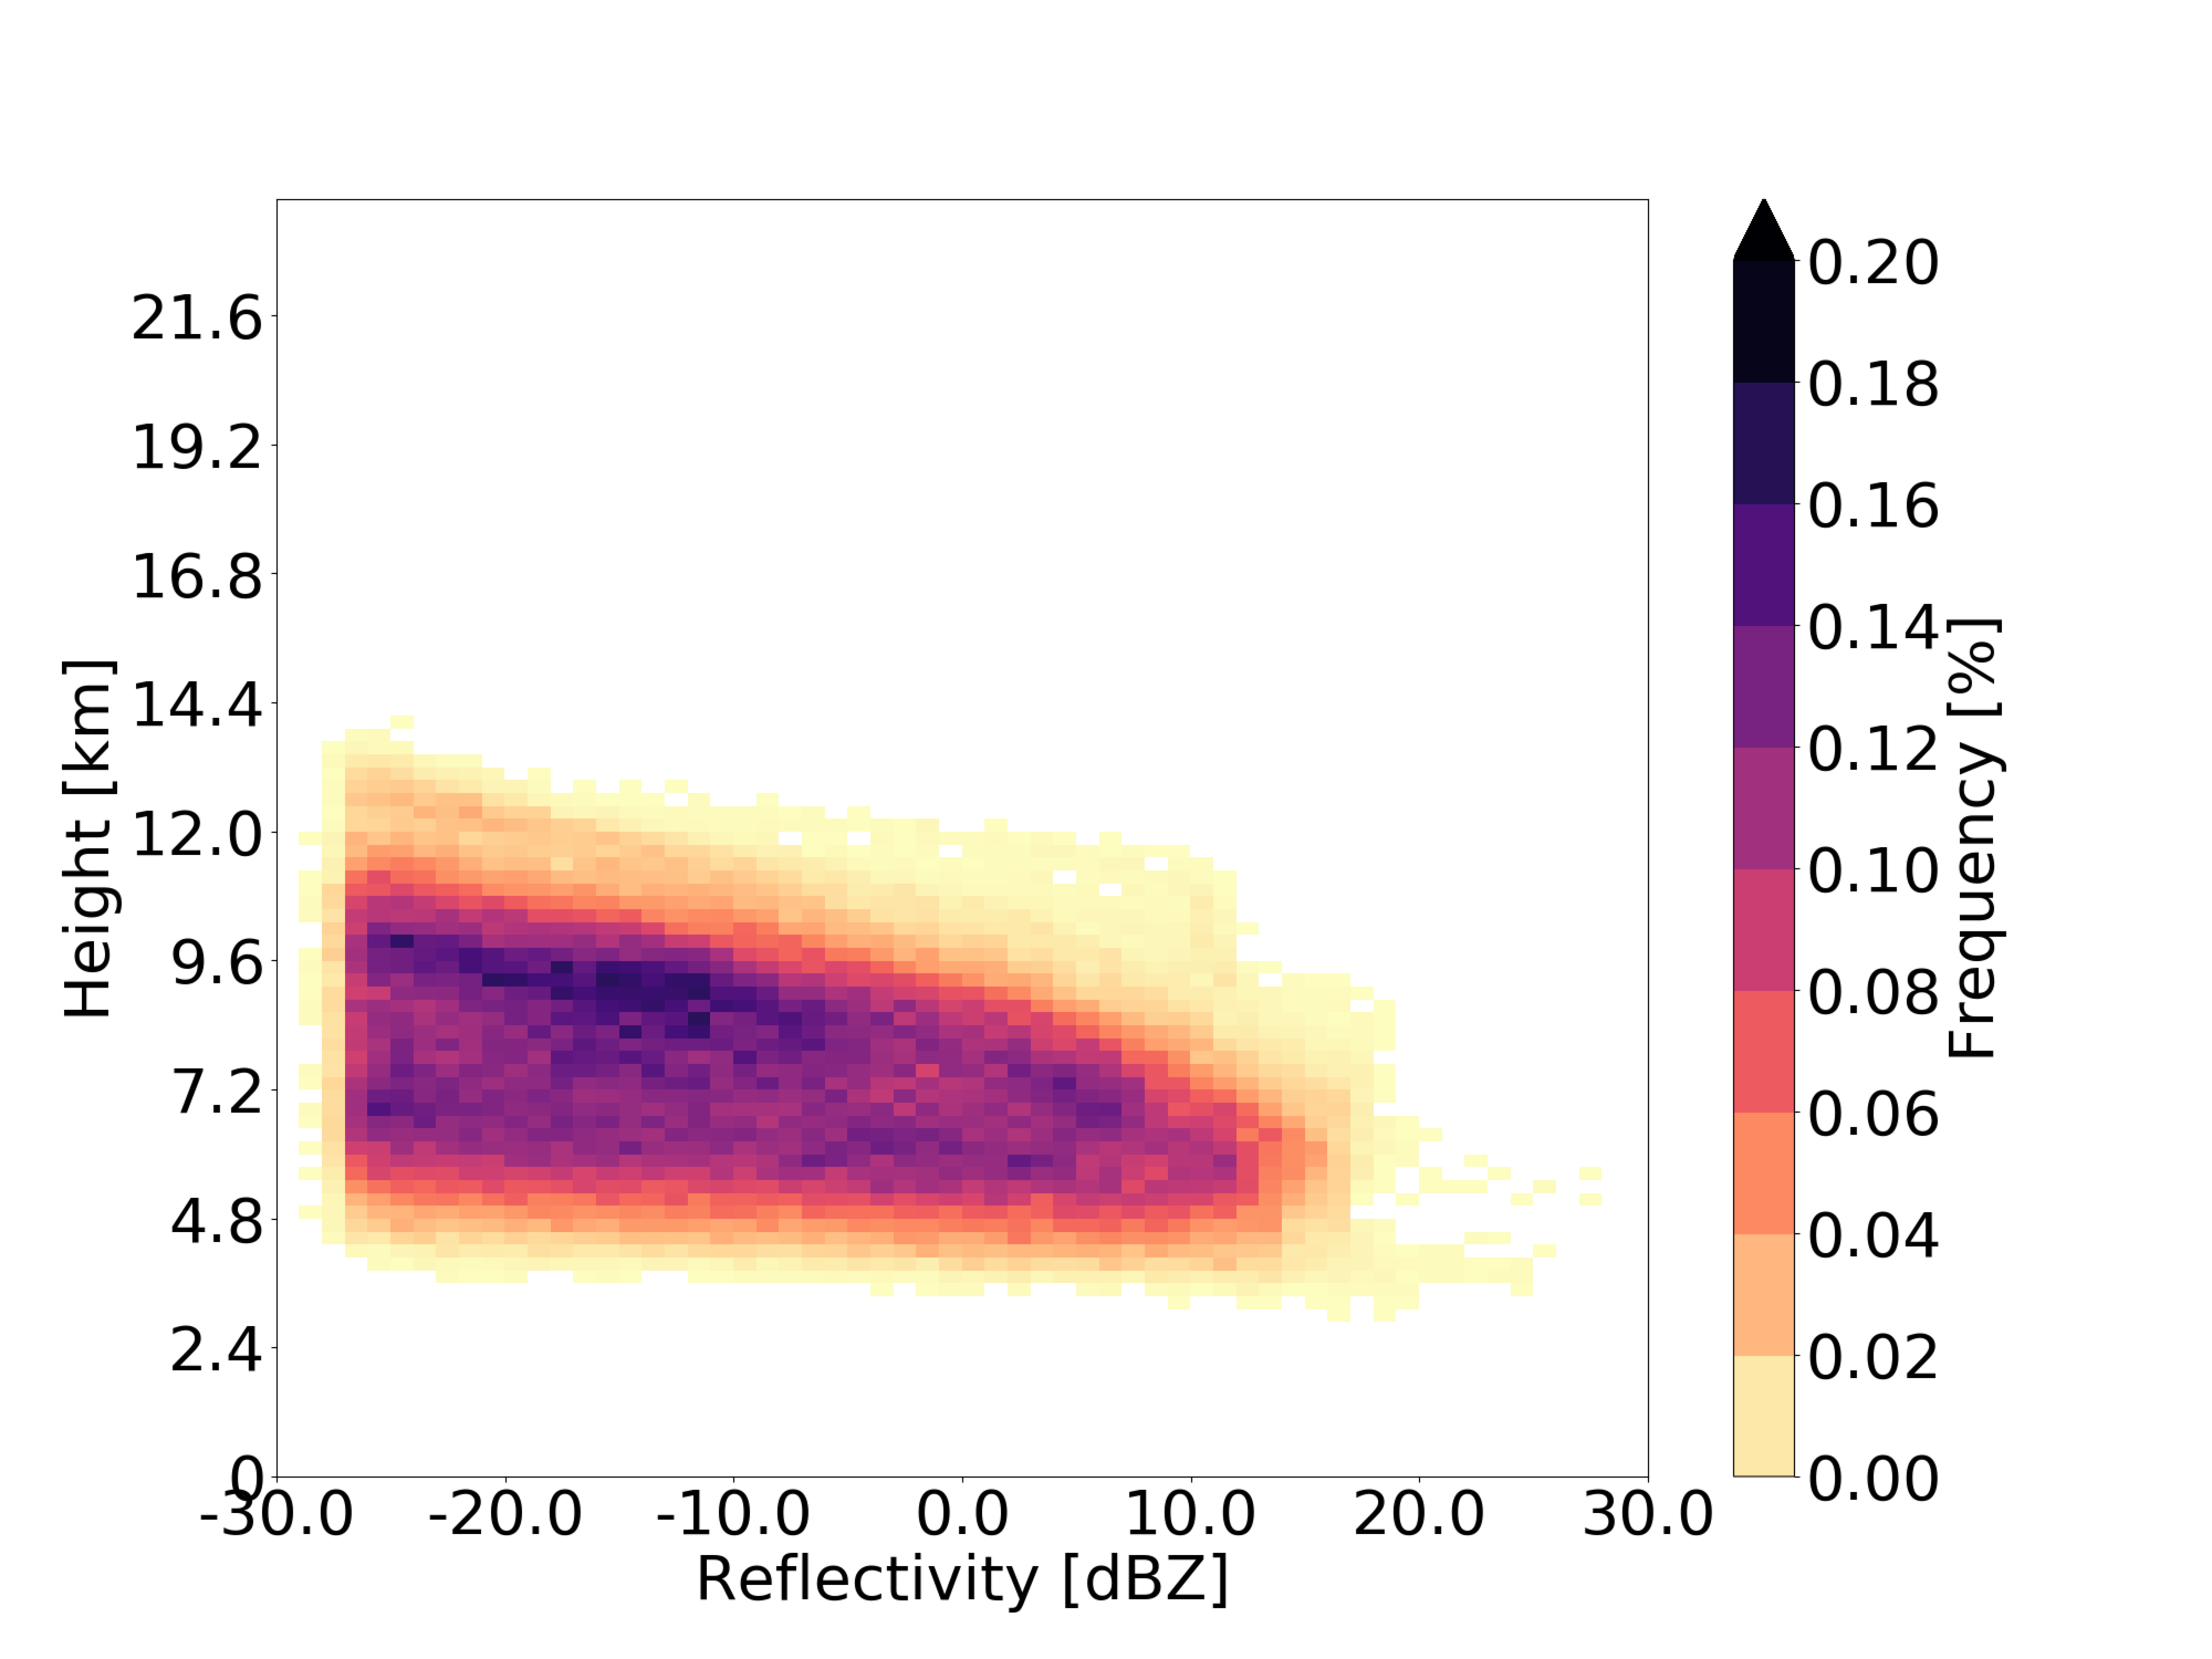
\includegraphics[width=\textwidth]{radar_reflect_monsoondomain_westerlyseason.png}
        \label{fig:CFAD4}
       \end{subfigure}%

    \begin{subfigure}[b]{0.5\textwidth}
       \centering
        \caption{westerly-dominated, May -- Sep}
        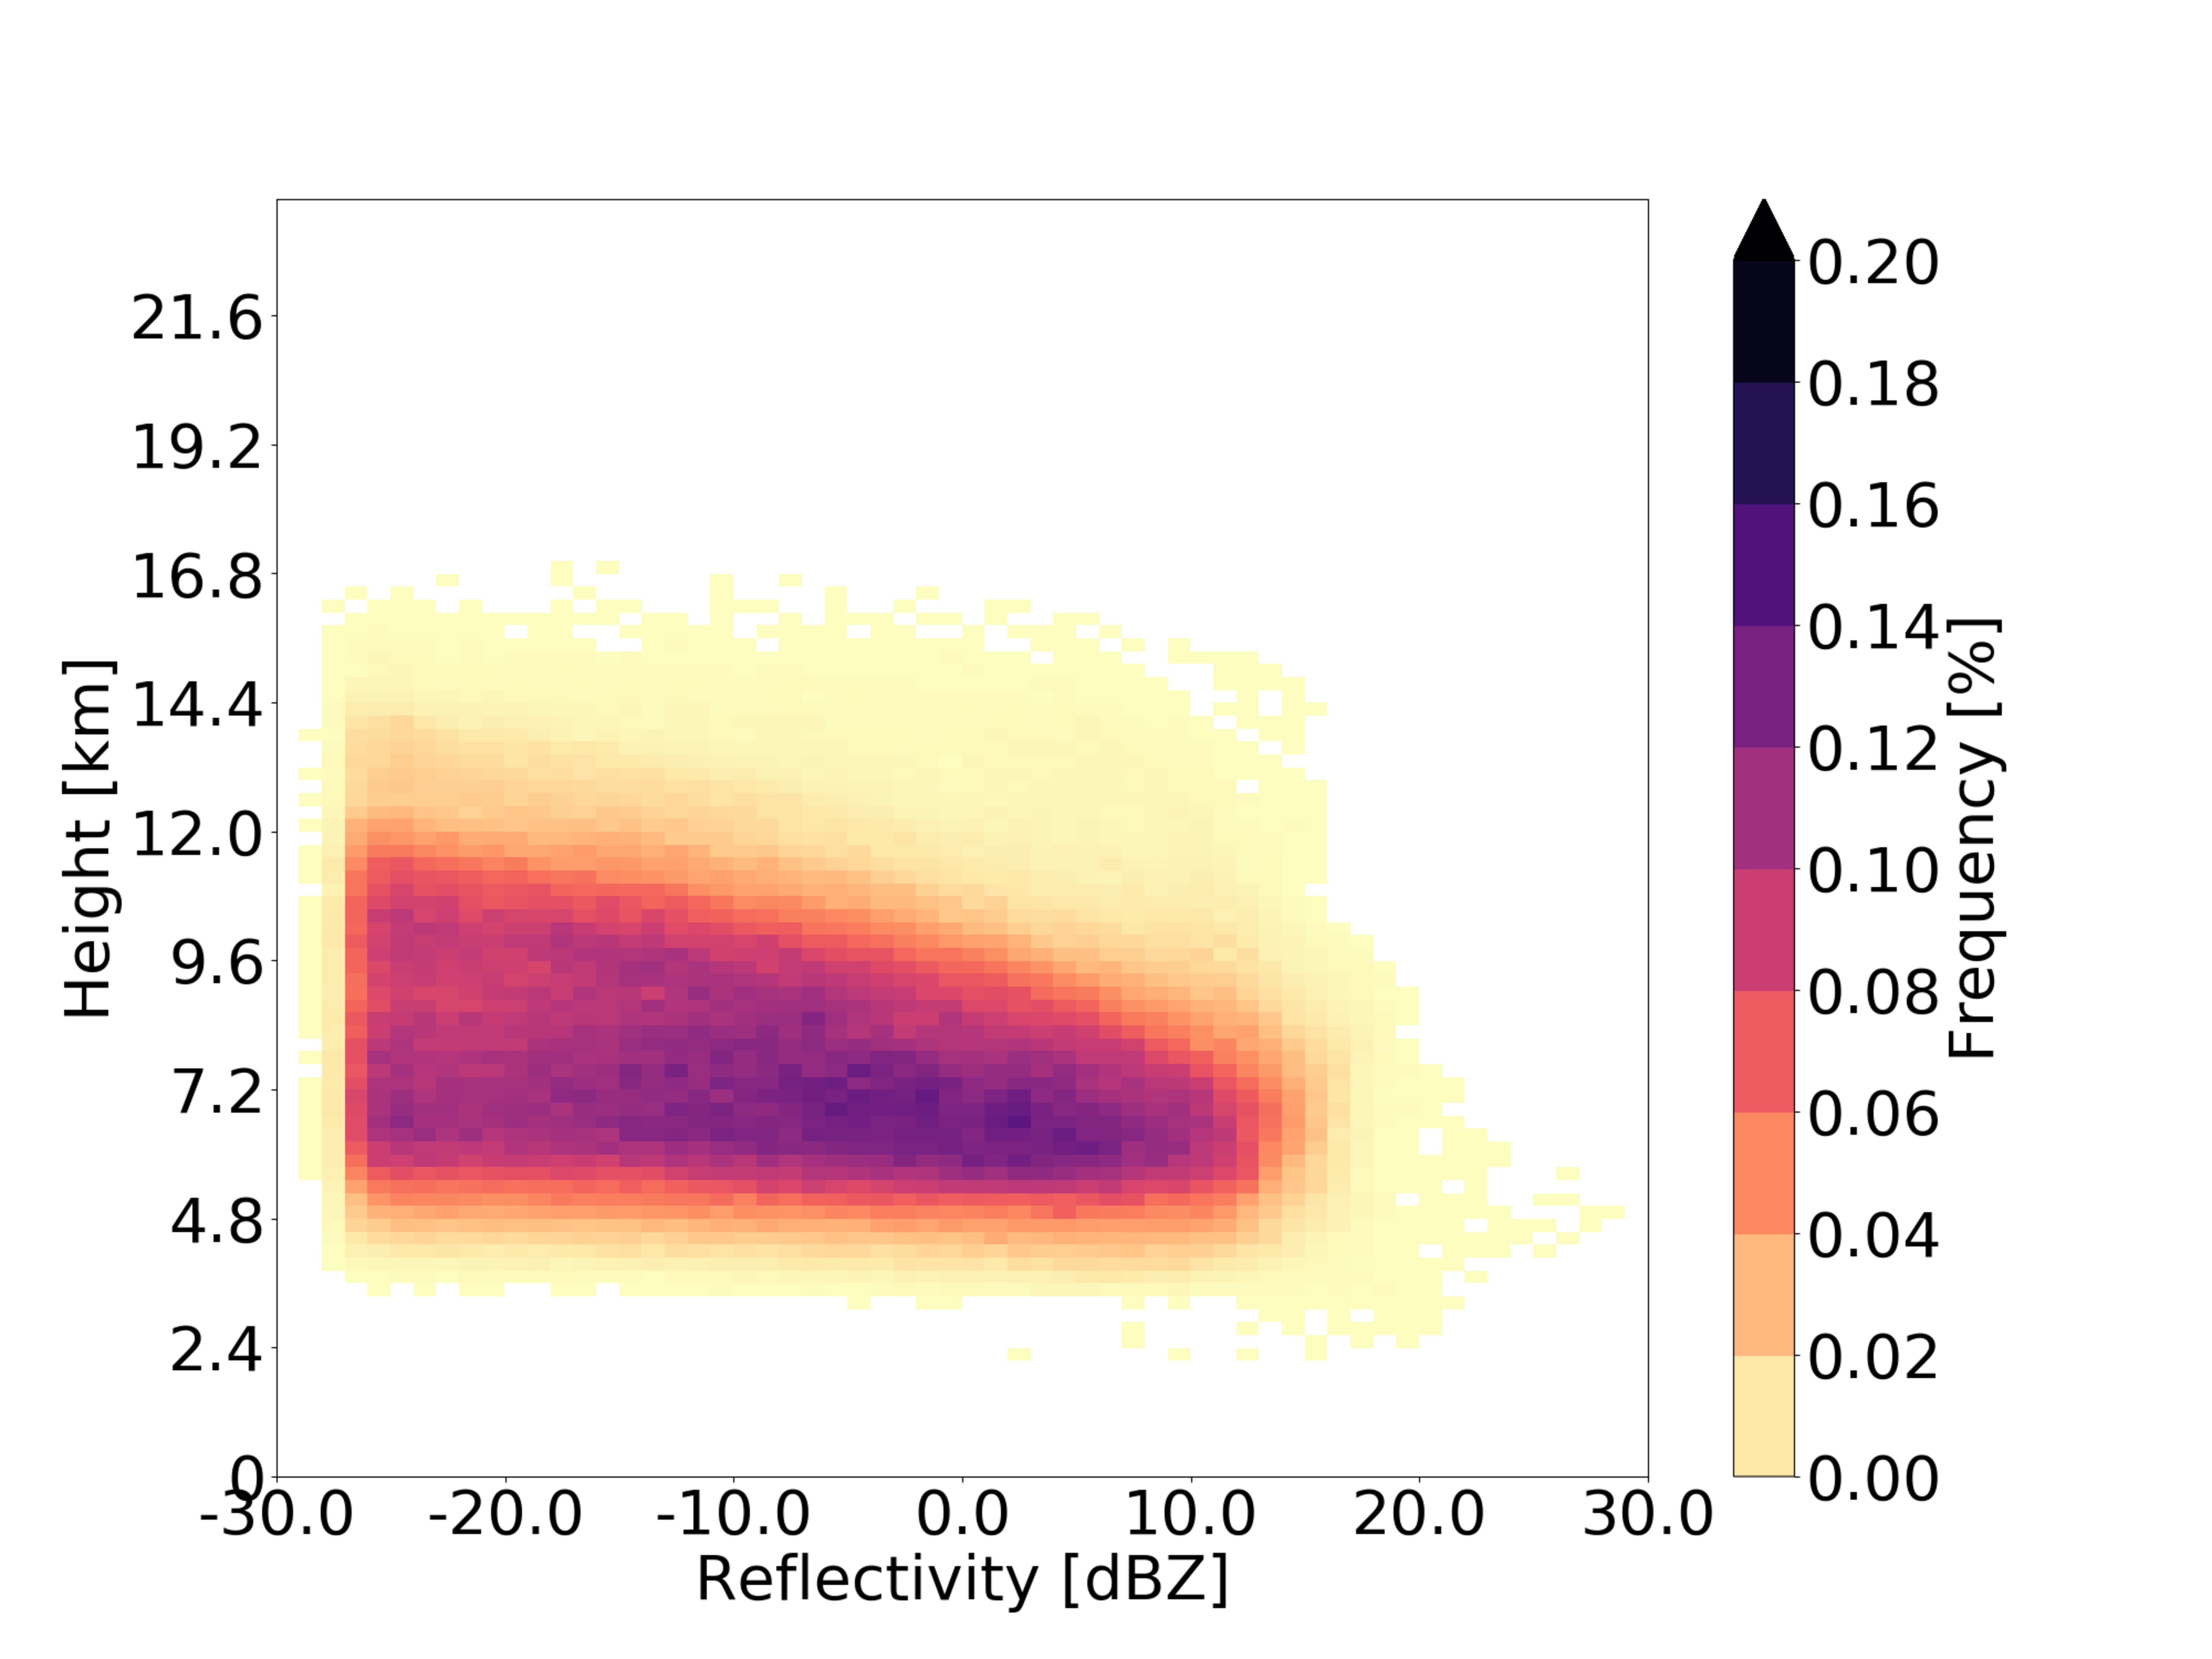
\includegraphics[width=\textwidth]{radar_reflect_westerlydomain_monsoonseason.png}
        \label{fig:CFAD5}
    \end{subfigure}%
    ~ 
    \begin{subfigure}[b]{0.5\textwidth}
        \centering
        \caption{westerly-dominated, Oct -- Apr}        
        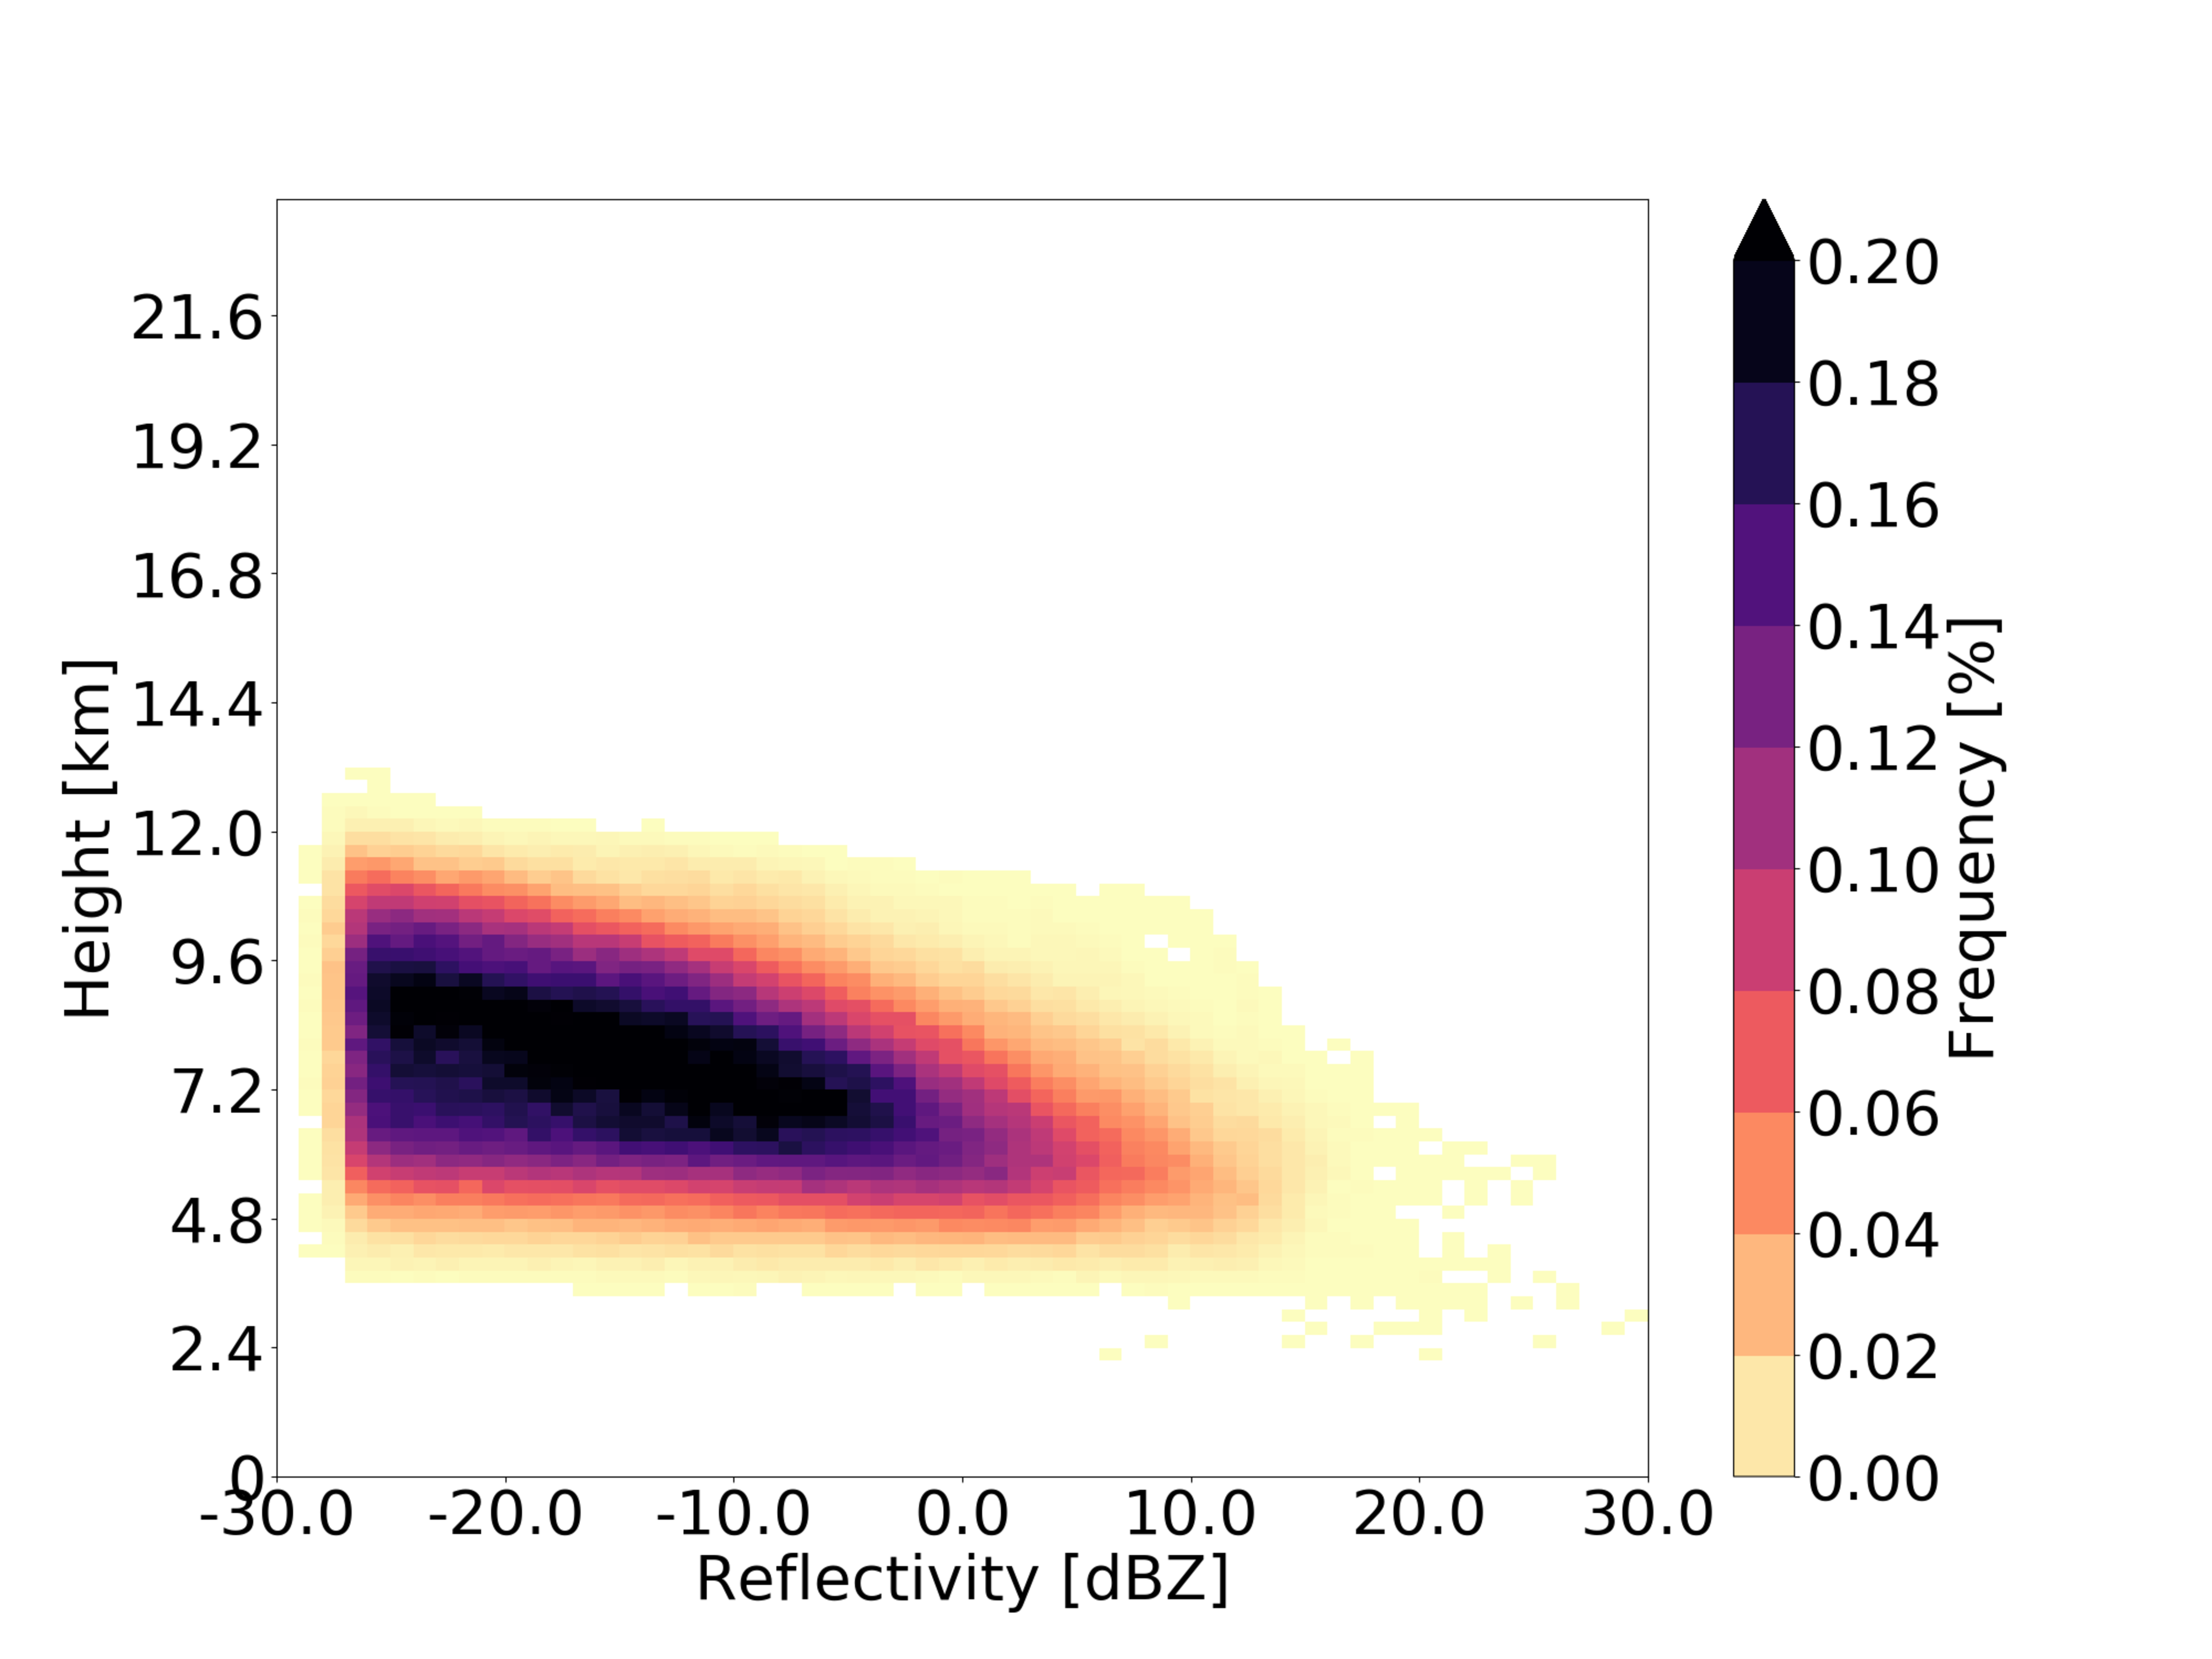
\includegraphics[width=\textwidth]{radar_reflect_westerlydomain_westerlyseason.png}
        \label{fig:CFAD6}
    \end{subfigure}
    \label{fig:CFAD}
    \end{figure}

\begin{figure}\ContinuedFloat
    \begin{subfigure}[t]{0.5\textwidth}
        \centering
        \caption{transition zone, May -- Sep }        
        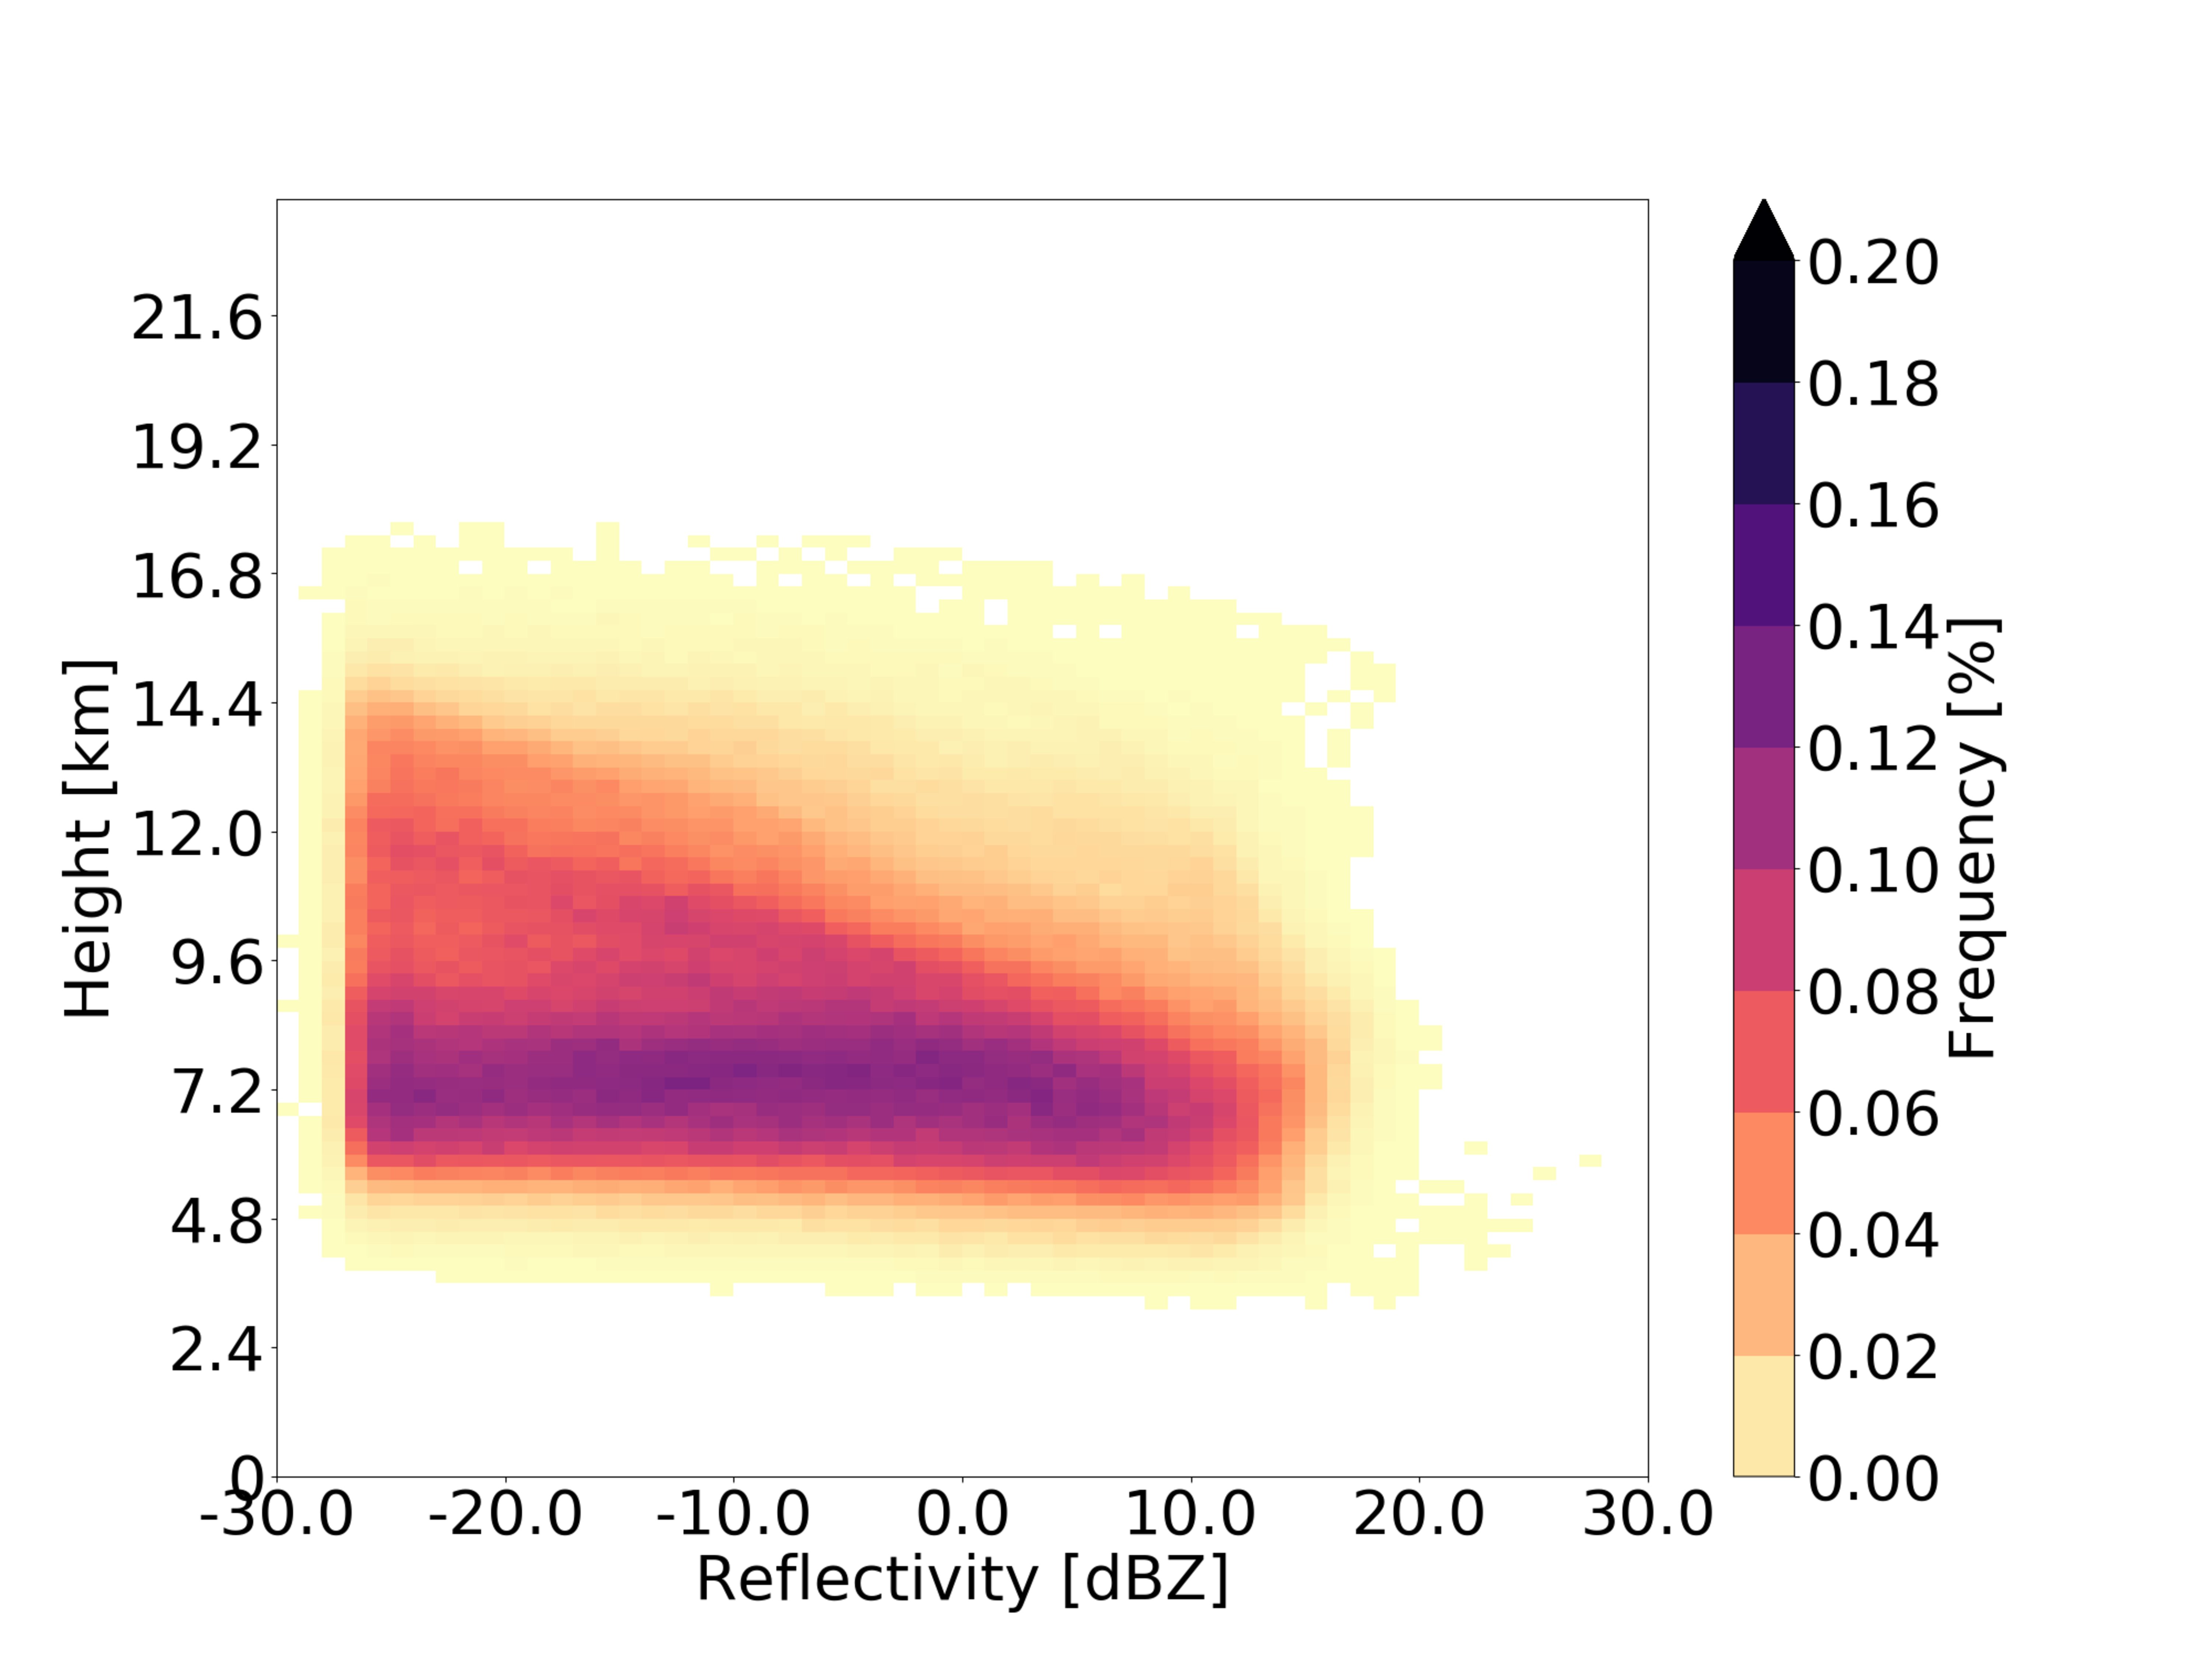
\includegraphics[width=\textwidth]{radar_reflect_transitionzone_monsoonseason.png}
\label{fig:CFAD7}
    \end{subfigure}%
    ~ 
    \begin{subfigure}[t]{0.5\textwidth}
        \centering
        \caption{transition zone, Oct -- Apr}        
        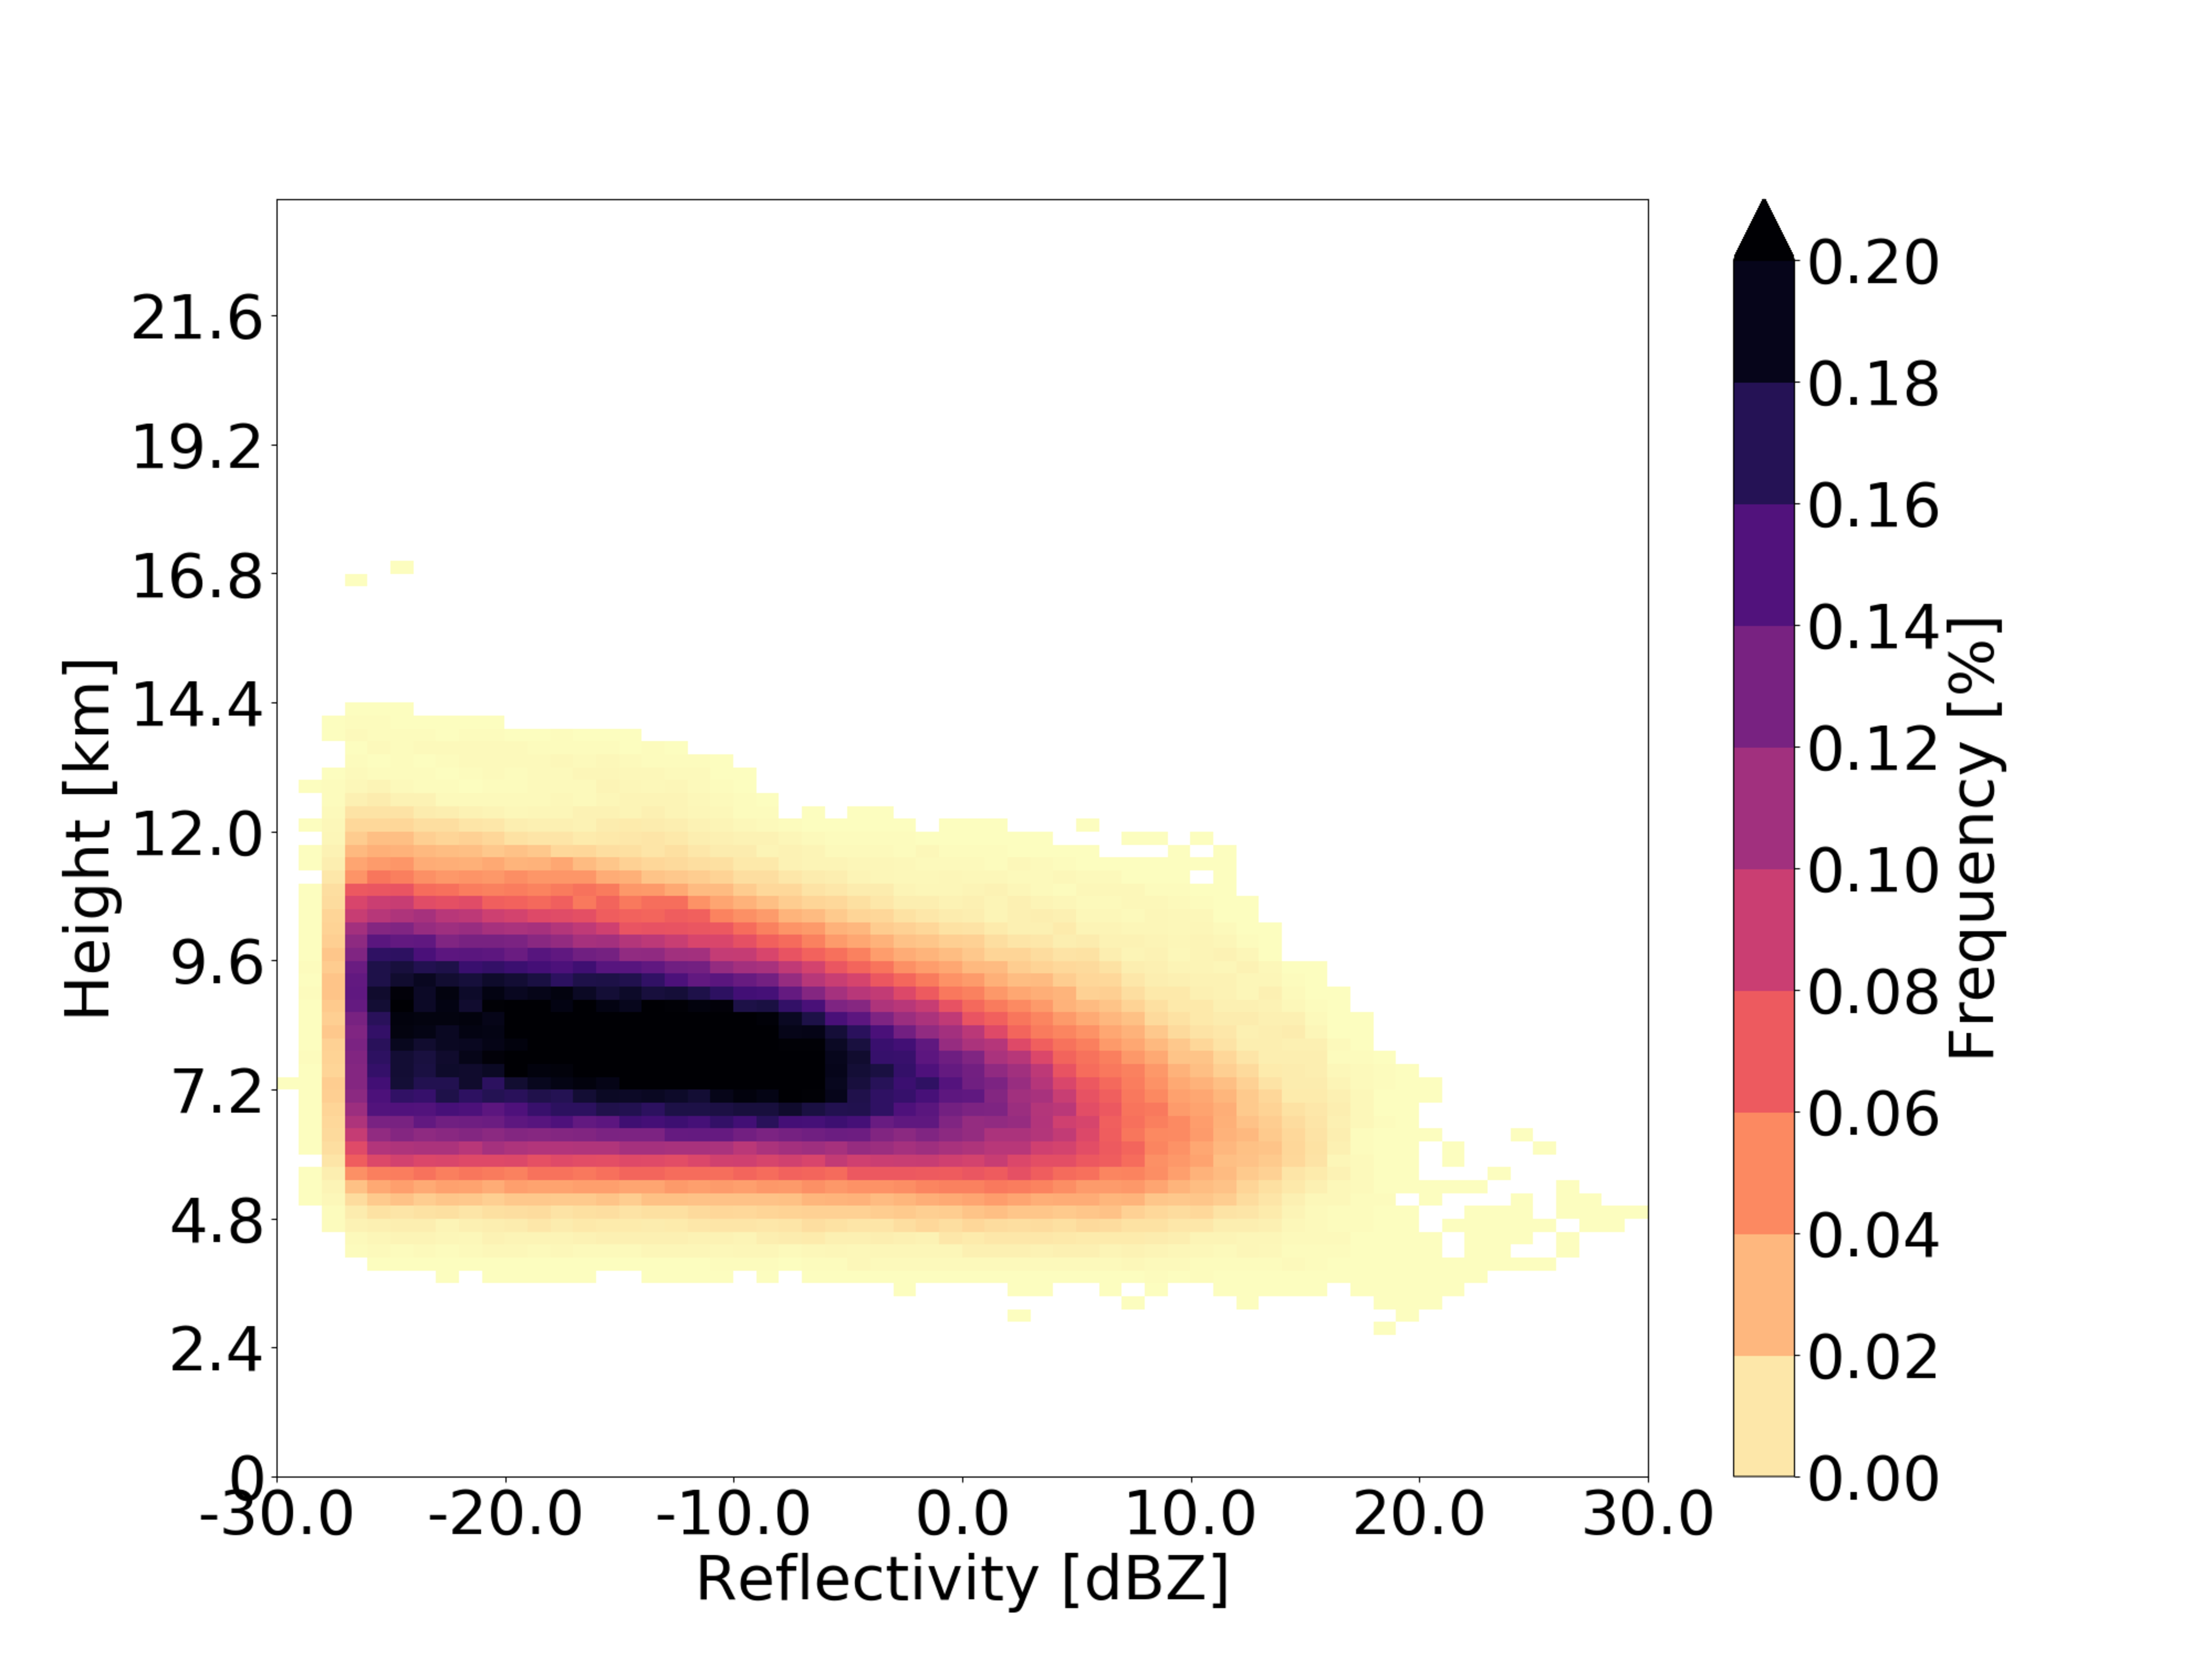
\includegraphics[width=\textwidth]{radar_reflect_transitionzone_westerlyseason.png}
        \label{fig:CFAD8}
        \end{subfigure}
    \caption[]{CFAD of radar reflectivity for TP domain (a -- b), monsoon-dominated domain (c -- d), westerly-dominated domain (e --f) and transition zone (g -- h) during monsoon (May--Sep) and westerly seasons (Oct--Apr) based on 2B-GEOPROF (2006 -- 2011). The height bin (km a.s.l.) ranges from 2 to 17 km with a 0.24 km interval, and the reflectivity bin (dBZ) ranges from -30 to 30 dBZ with a 1 dBZ intervals.}
    \label{fig:CFAD}
\end{figure}


The higher variation of cloud layer types, cloud fractions and particle sizes at different heights during the monsoon (as shown in the previous section) is not necessarily attributed to single cloud layers during one satellite overpass, because \textit{CPR} can detect up to five cloud layers in one sampled profile (Section 2). The frequencies of multiple cloud layers (\% of all profiles which at least contain one cloud layer) is therefore presented in Figure \ref{fig:seasonal_cld_lyr}. In general, single-layer clouds are the most frequent cloud layer type in the whole TP domain, contributing between 50 and 85 \% to the total cloud layer detections (Fig. \ref{fig:seasonal_cld_lyr1}). The relative contribution of single layer clouds shows a strong seasonal dependence in the monsoon-dominated south and decreases during the monsoon months, especially in July and August (Fig. \ref{fig:seasonal_cld_lyr2}). Multiple cloud layer occurrences are most frequent in the monsoon-dominated domain (Fig. \ref{fig:seasonal_cld_lyr2}) and during the monsoon months in all regions. The highest contribution of two-layer clouds are observed between May and September during night in the monsoon-dominated domain, which is consistent with the vertical cloud fractions revealing the co-occurrence of high level cirrus clouds and low level clouds in the summer nighttime profiles (cf. Section 4.2). In the westerly-dominated domain, two-layer clouds are most frequent in March (Fig. \ref{fig:seasonal_cld_lyr4}) and the transition zone shows again properties of both the westerly-dominated and monsoon-dominated domain. The number of detected cloud layers during nighttime is smaller than during daytime in all regions during all months (except for July in the monsoon-dominated domain). However, the nighttime curves for cloud layer amount frequencies follow the daytime curves and the monthly variation of cloud layer amount outweighs the day-night differences. 


\begin{figure}[!htbp]
    \begin{subfigure}[b]{0.5\textwidth}
       \centering
        \caption{TP day}
        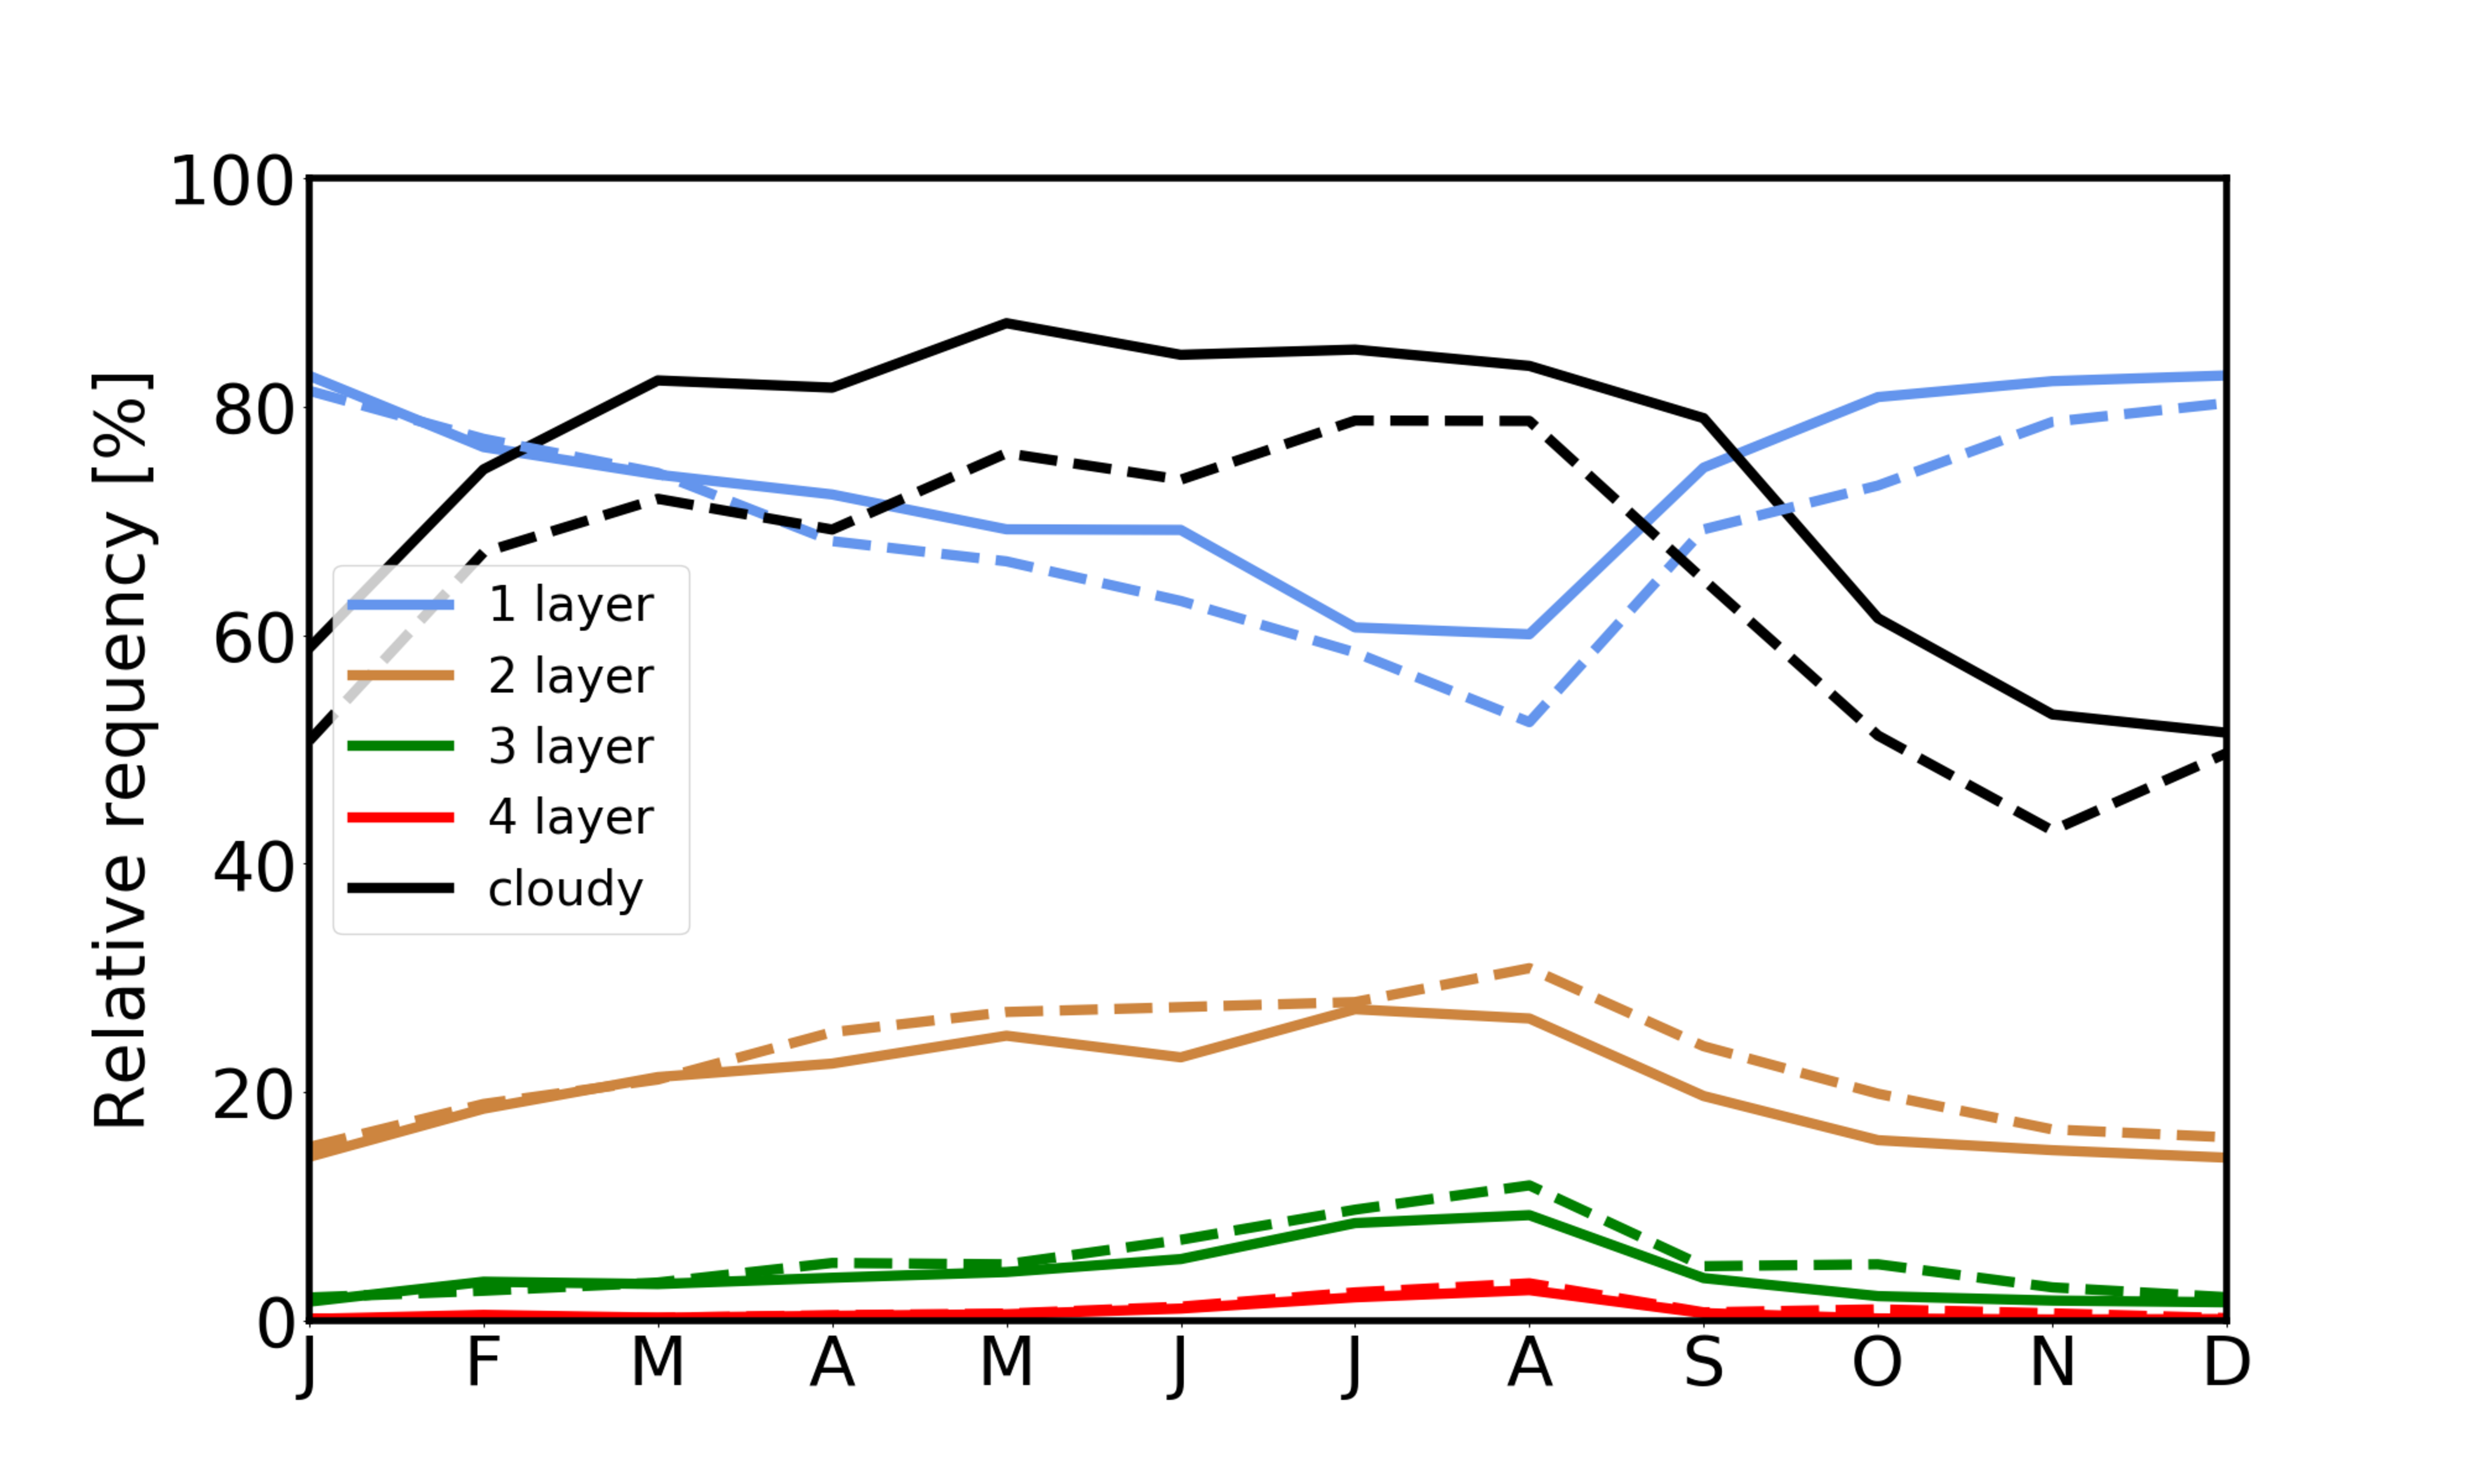
\includegraphics[width=\textwidth]{monthly_cld_layer_TP.png}
\label{fig:seasonal_cld_lyr1}
    \end{subfigure}%
    ~ 
    \begin{subfigure}[b]{0.5\textwidth}
        \centering
        \caption{monsoon-dominated}        
        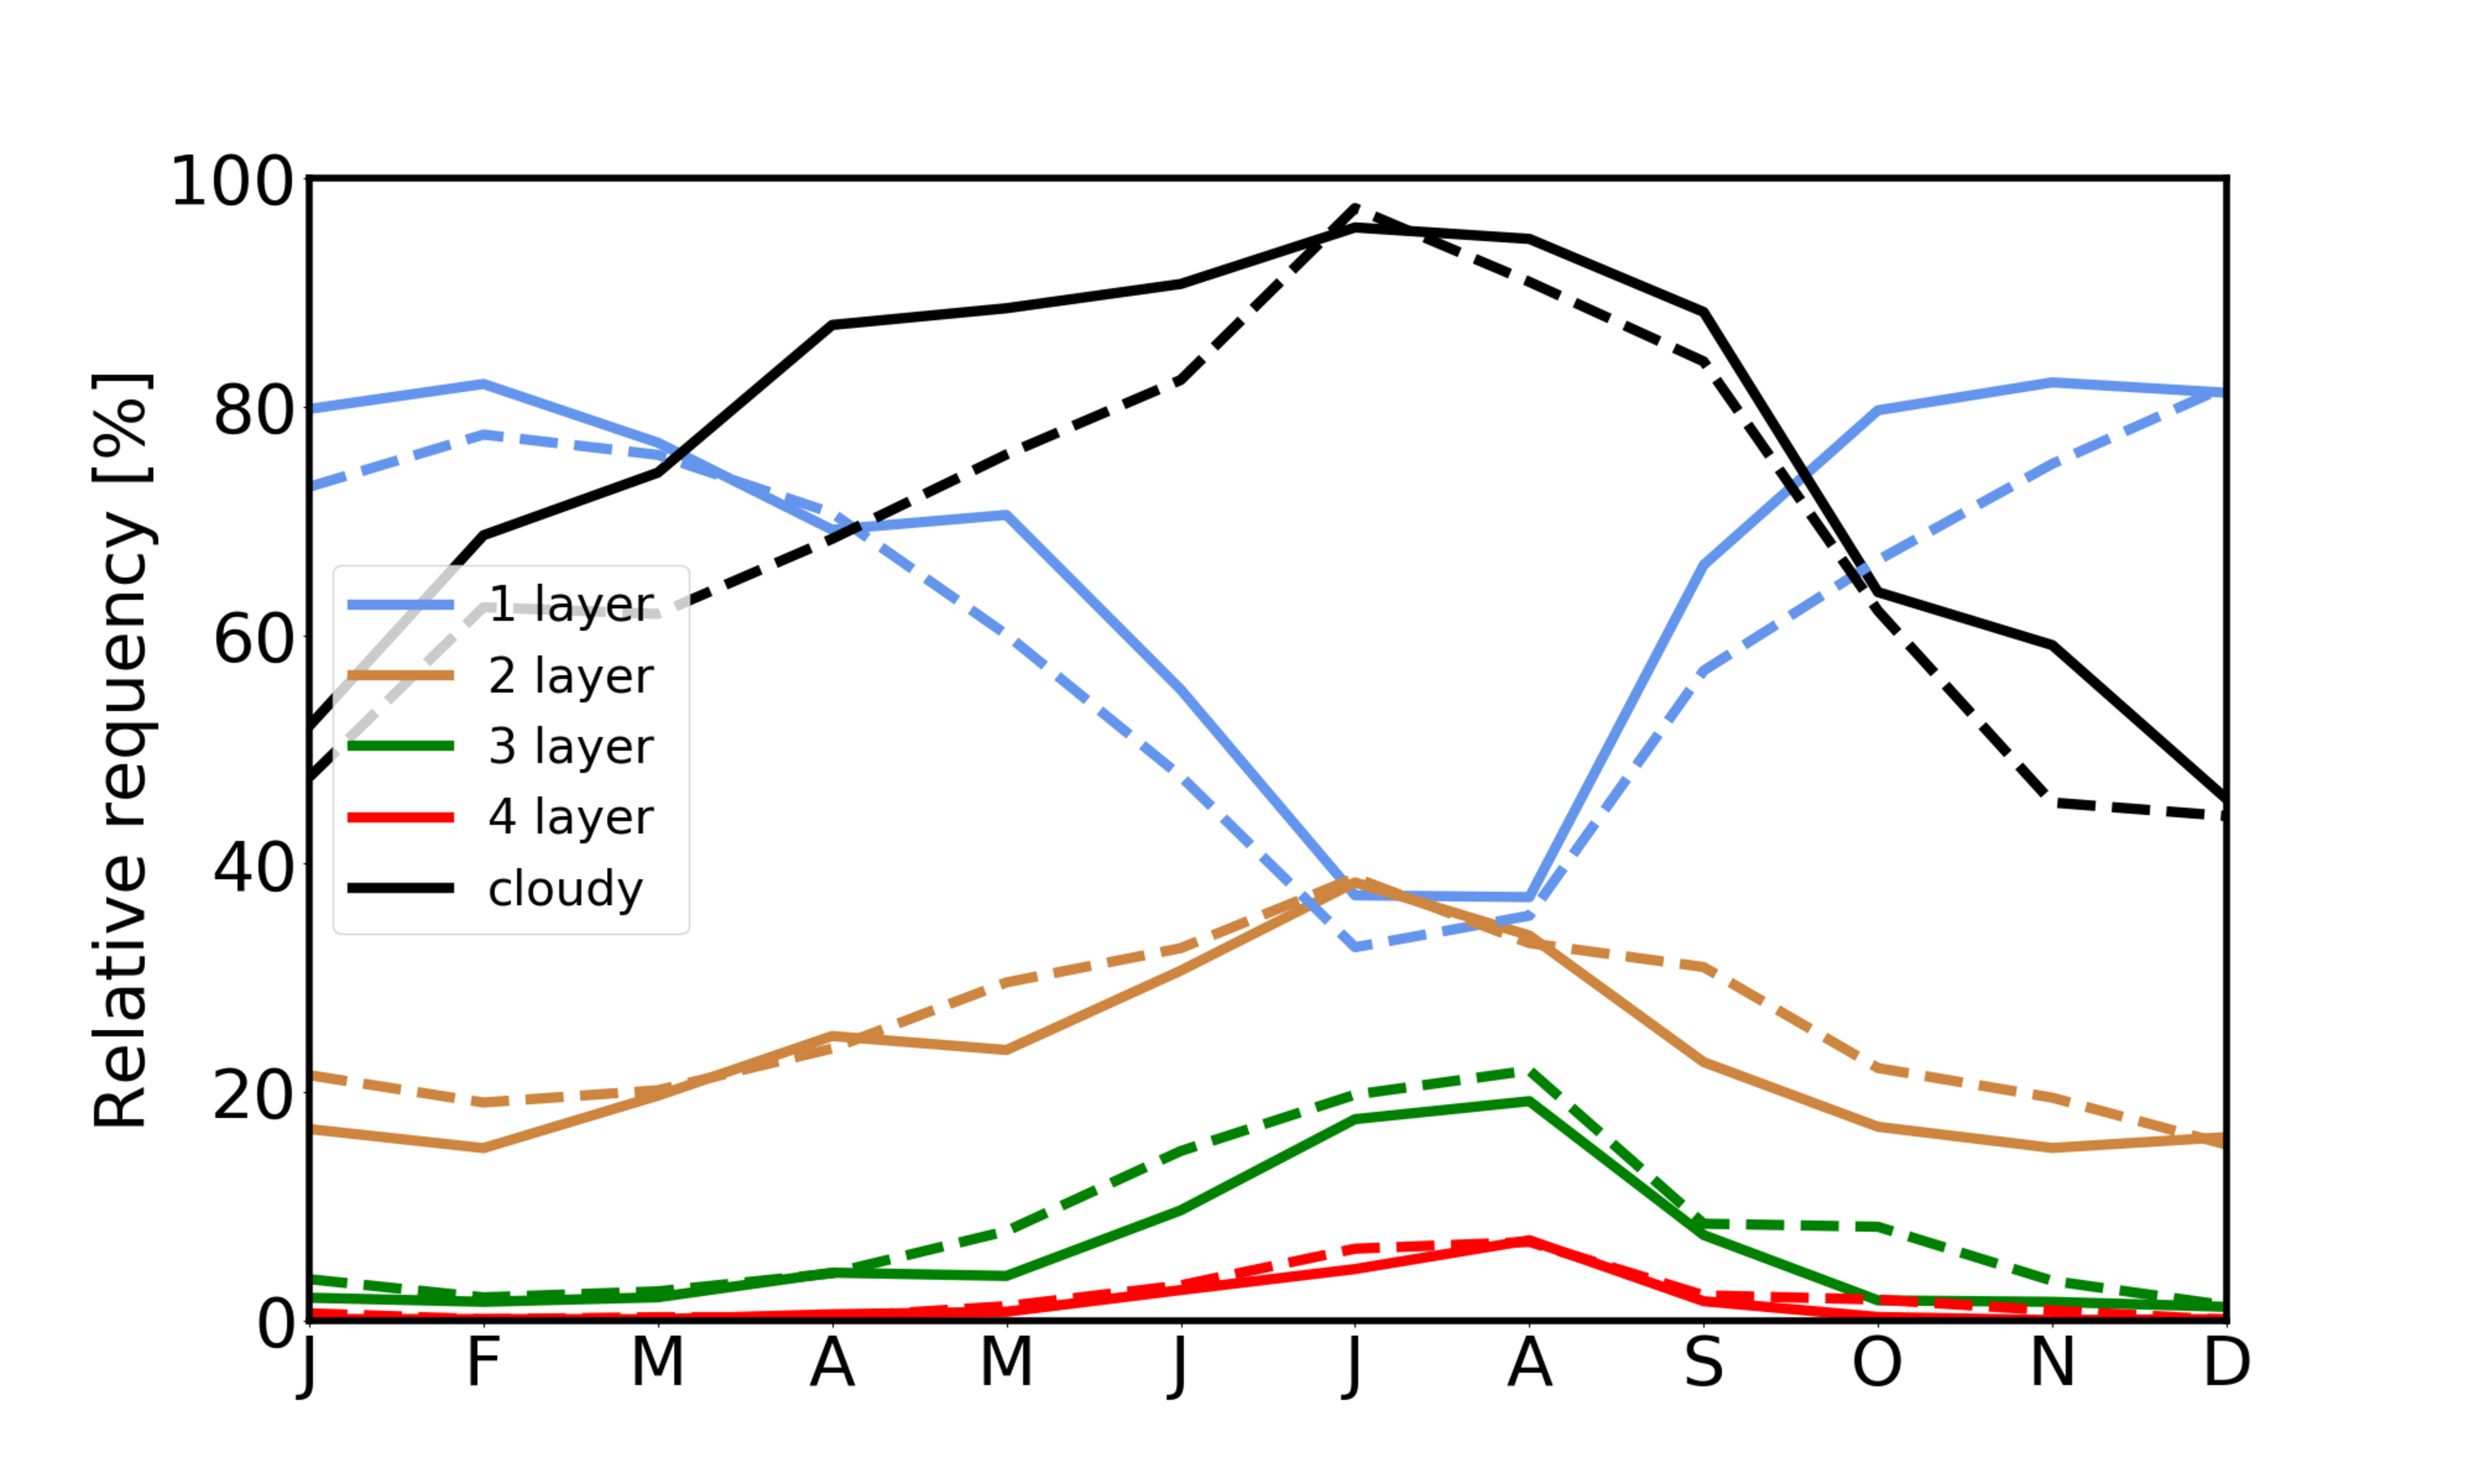
\includegraphics[width=\textwidth]{monthly_cld_layer_monsoon_region.png}
\label{fig:seasonal_cld_lyr2}
    \end{subfigure}
    
    \bigskip

    \begin{subfigure}[b]{0.5\textwidth}
        \centering
        \caption{transition zone }        
        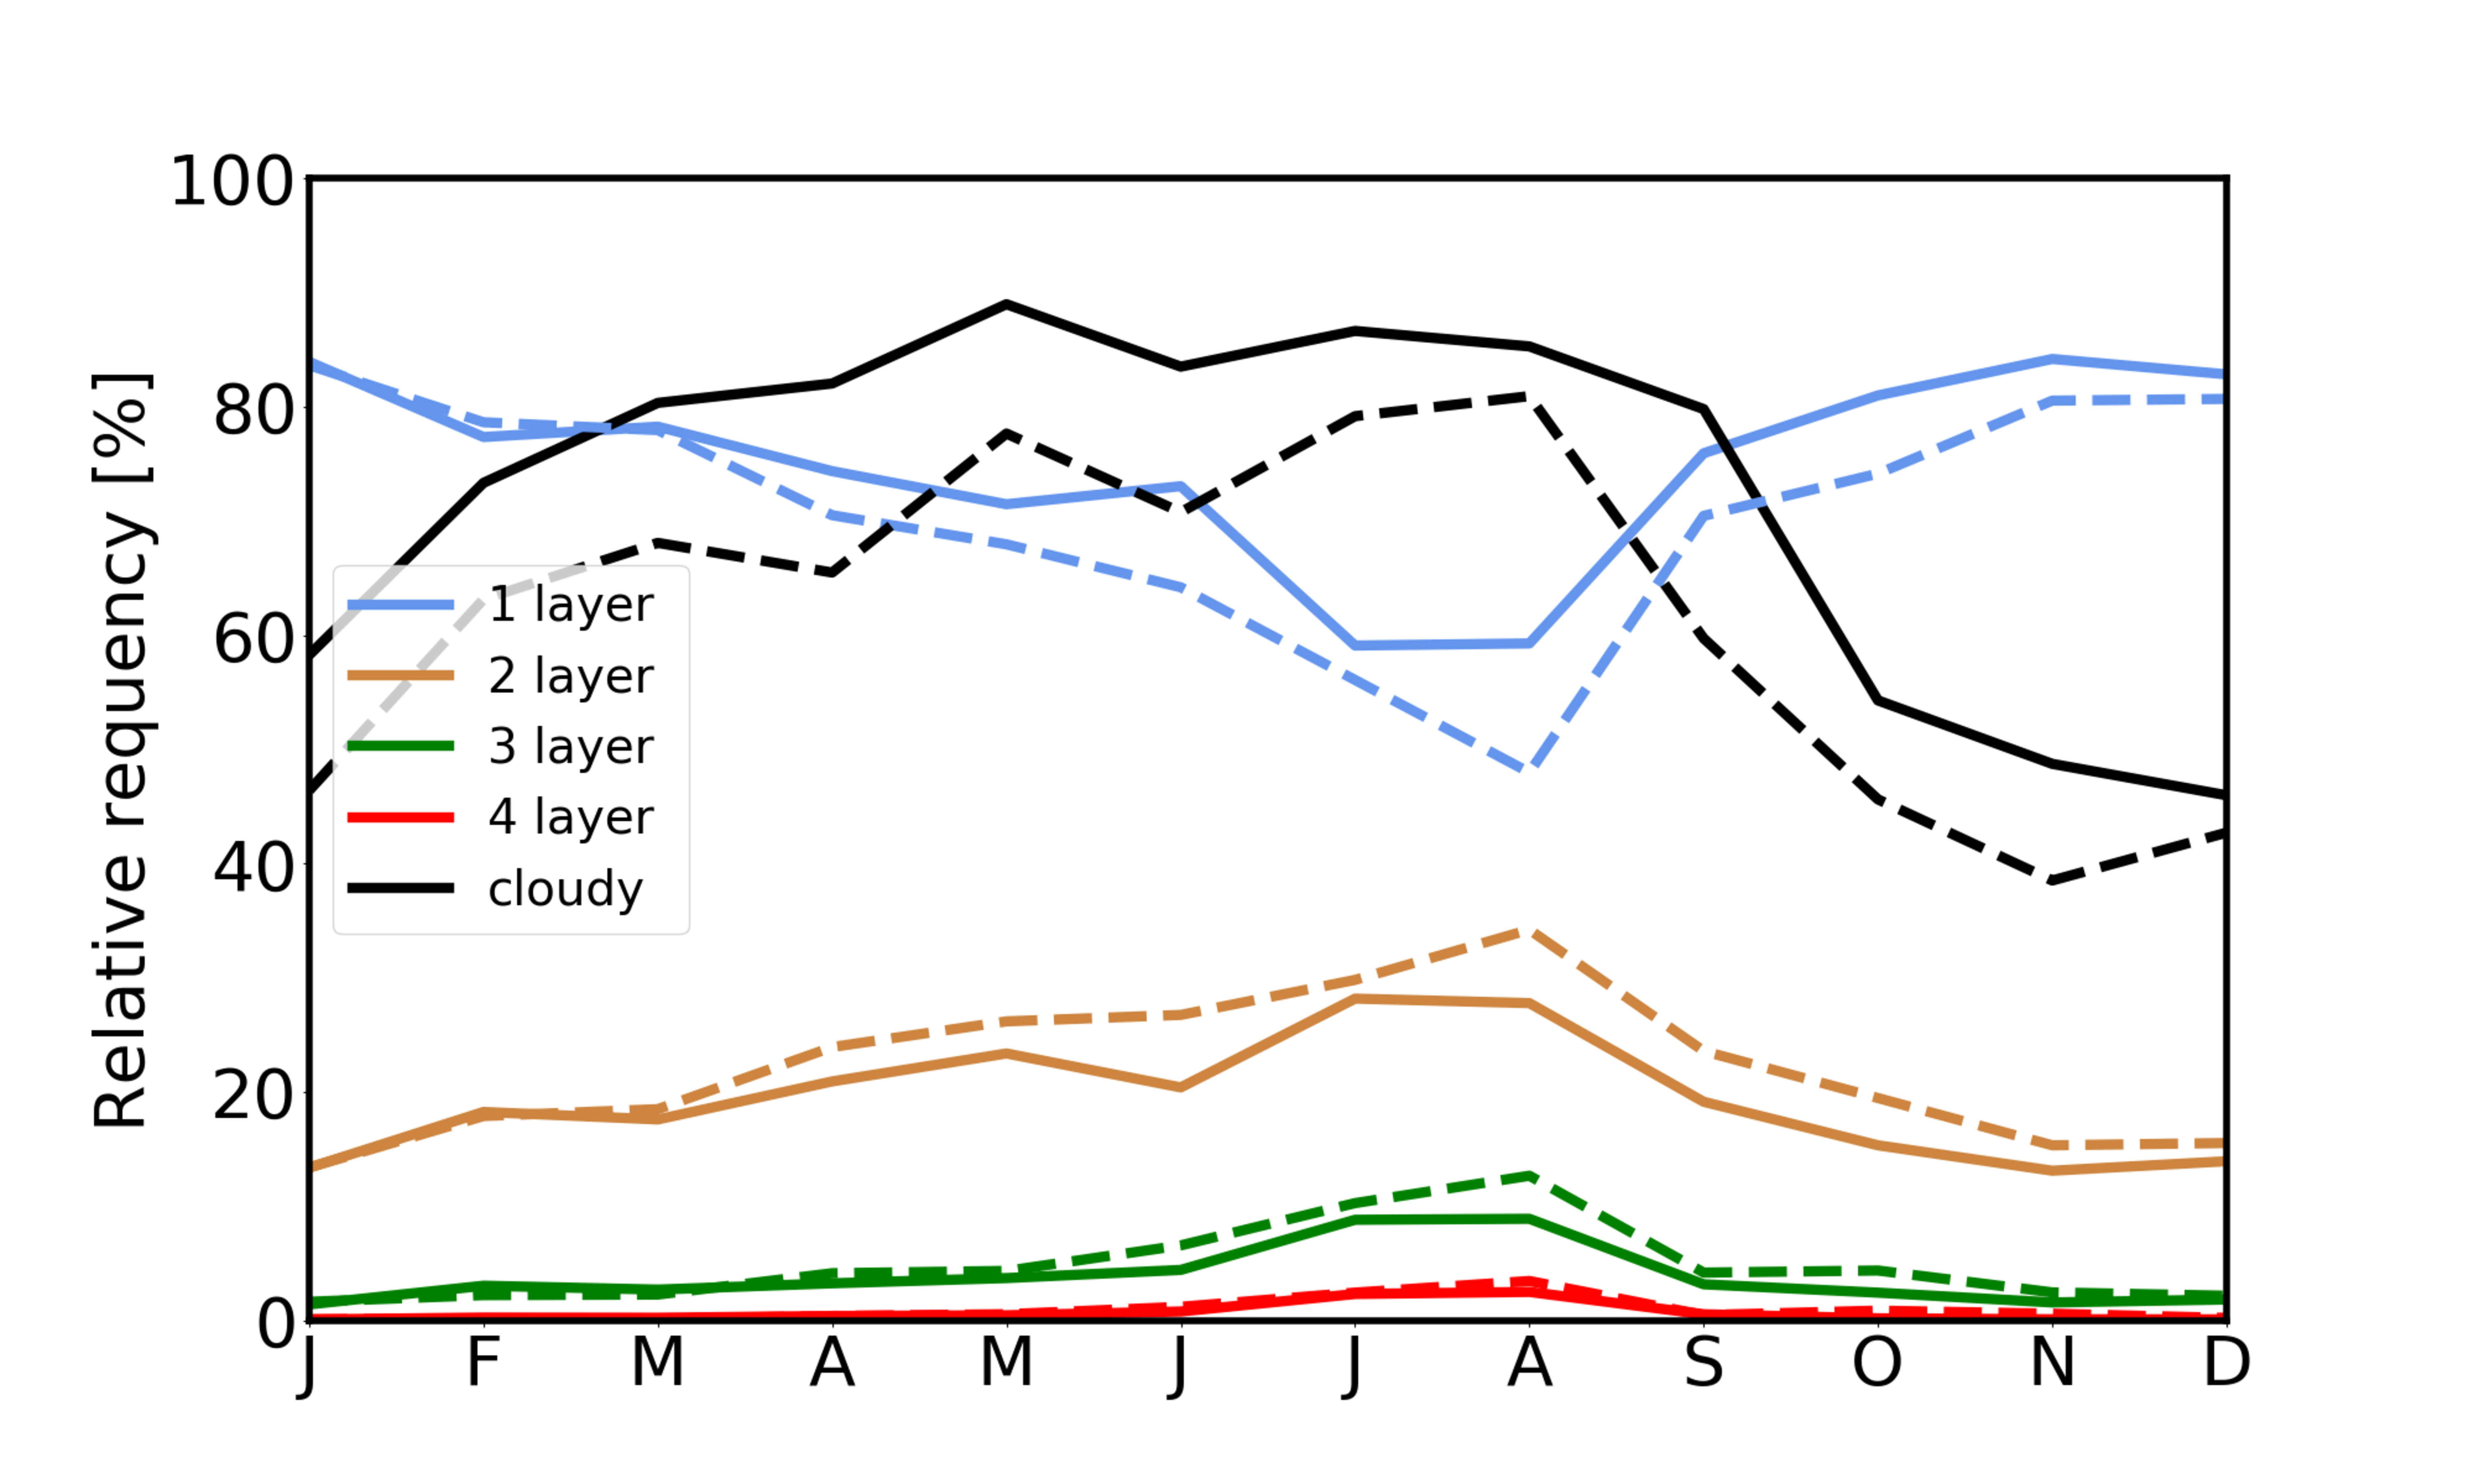
\includegraphics[width=\textwidth]{monthly_cld_layer_transition_region.png}
\label{fig:seasonal_cld_lyr3}
    \end{subfigure}%
    ~ 
    \begin{subfigure}[b]{0.5\textwidth}
        \centering
        \caption{westerly-dominated }        
        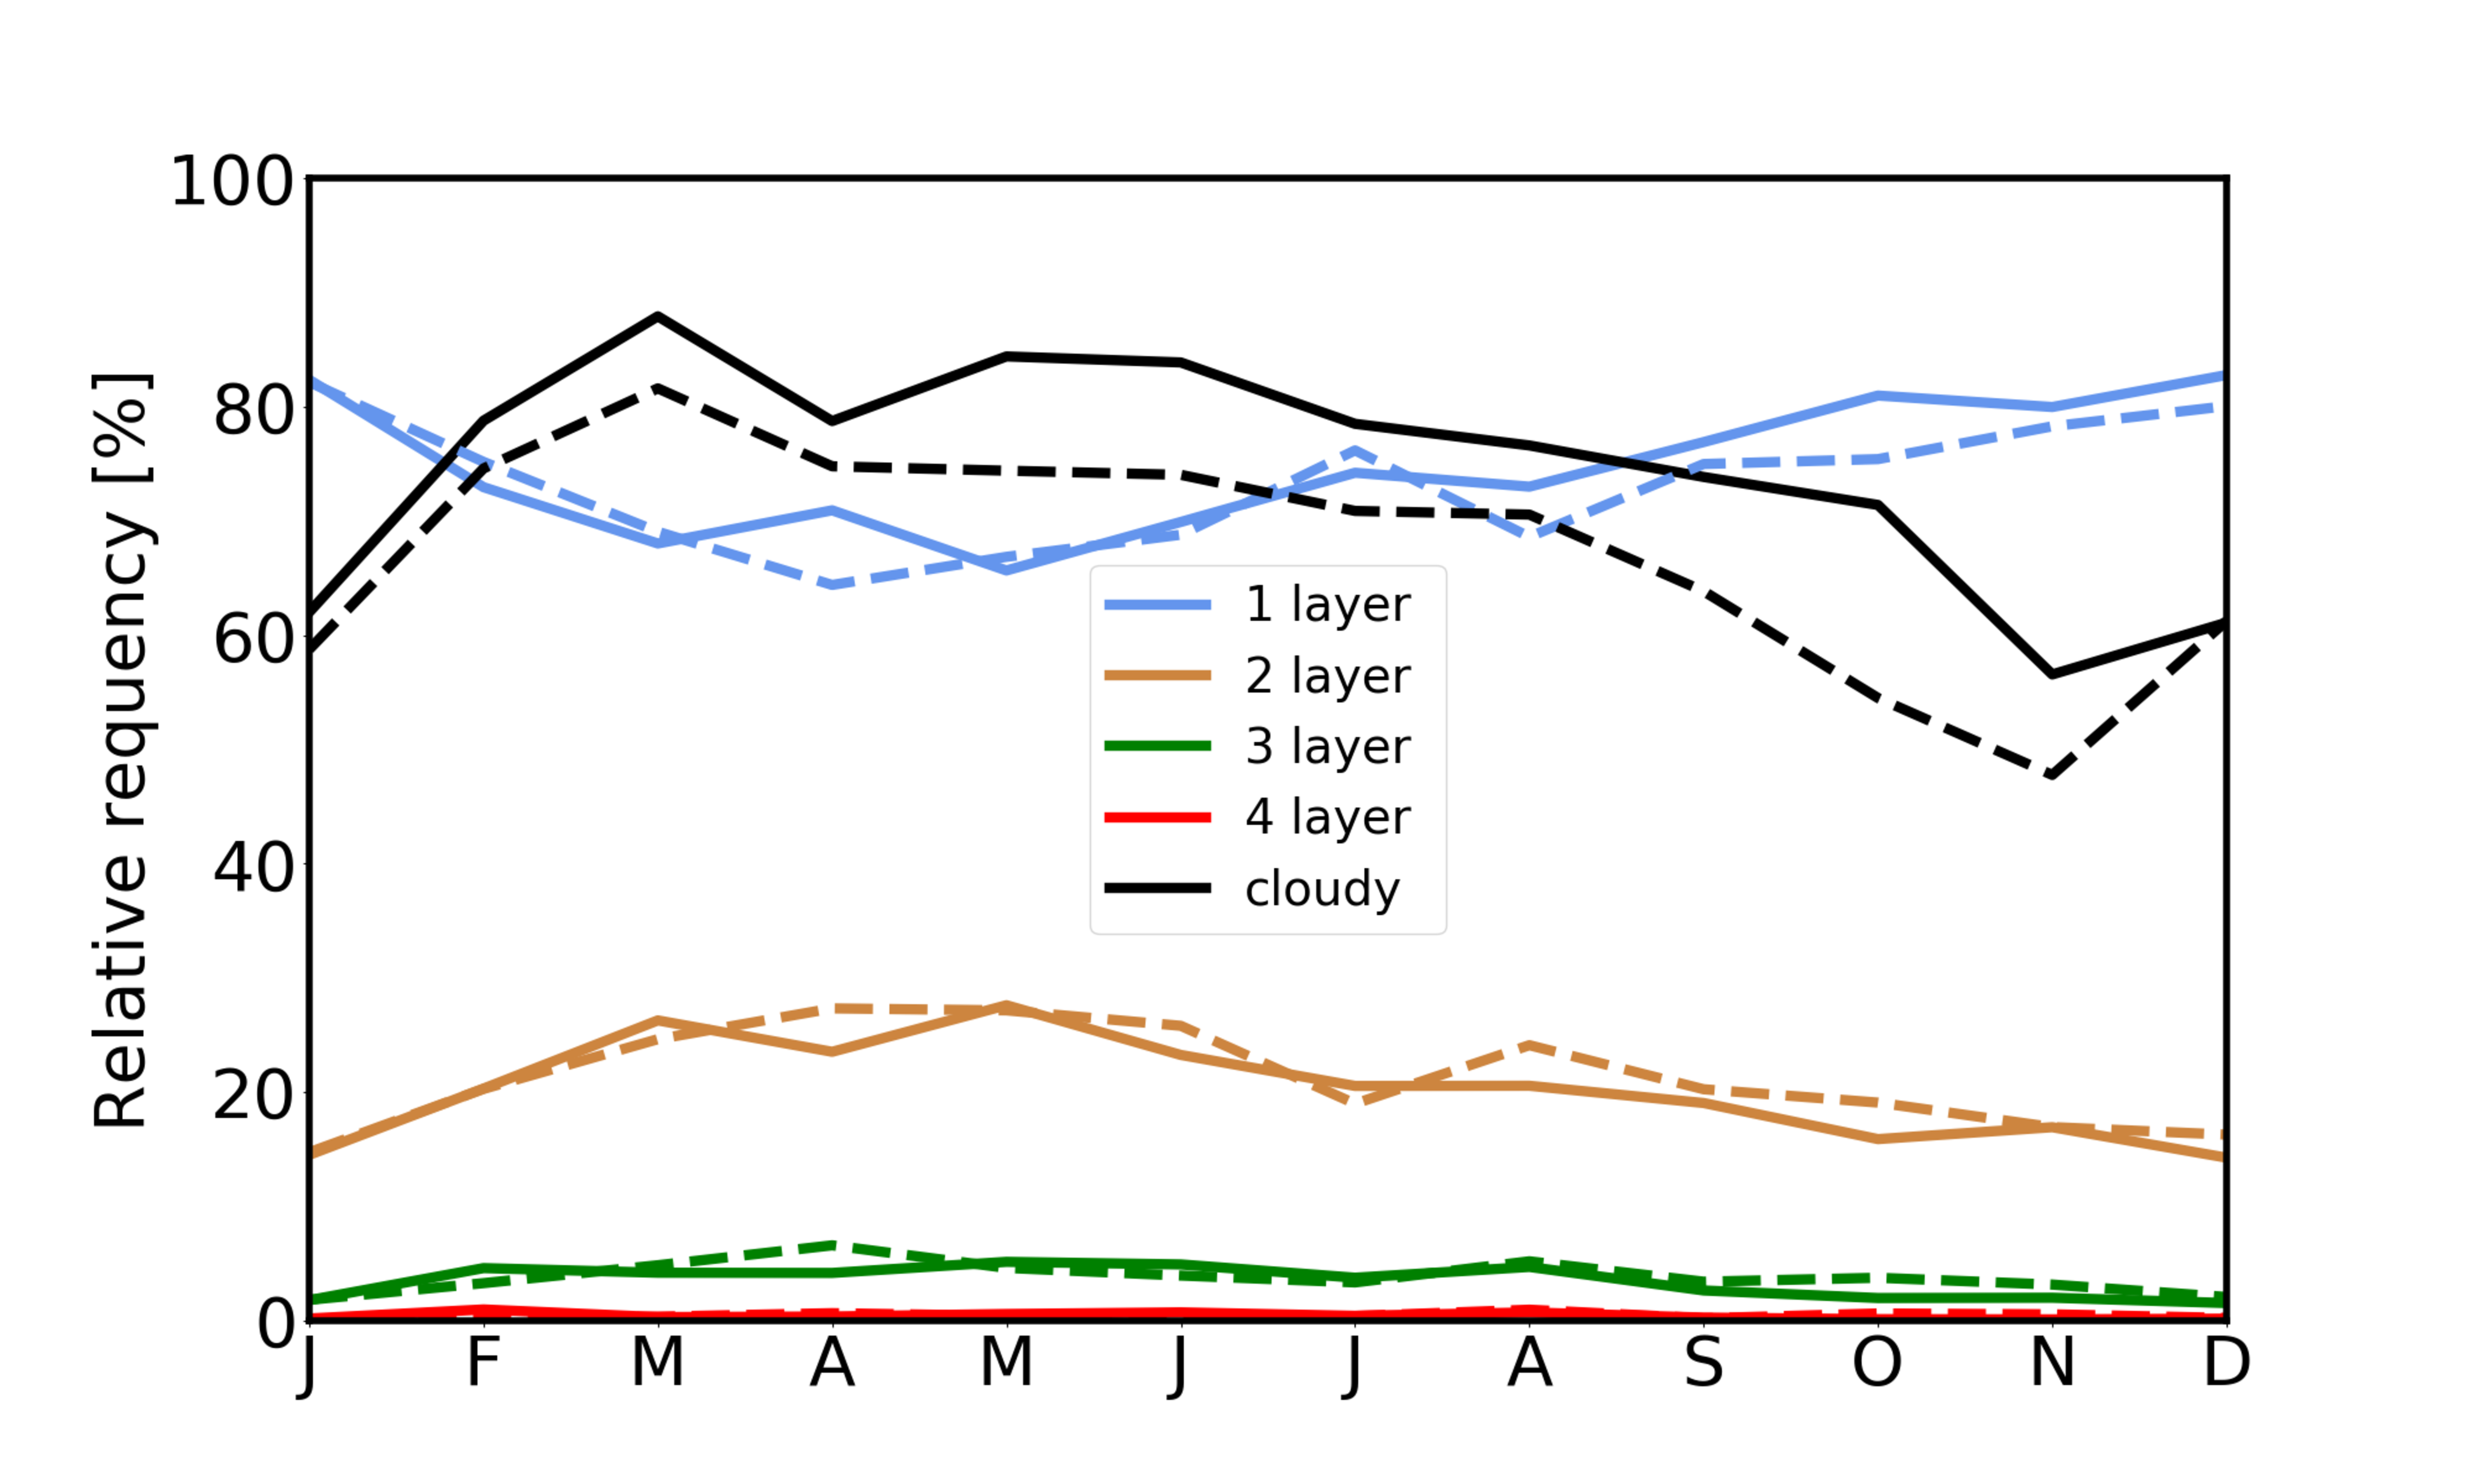
\includegraphics[width=\textwidth]{monthly_cld_layer_westerly_region.png}
        \label{fig:seasonal_cld_lyr4}
    \end{subfigure}  
\caption{Monthly variation of detected cloud layer amount (\% of profiles with at least one cloud layer) in the TP domain (a), monsoon-dominated domain (b), westerly-dominated domain (c) and transition zone (d) based on 2B-CLDCLASS-LIDAR (2007 -- 2010). The solid lines show the relative occurrence frequencies in daytime profiles and the dashed lines represent the nighttime profiles. The black curve refers to the occurrence frequency of samples that contain at least one detected cloud layer relative to all samples.}
\label{fig:seasonal_cld_lyr}
\end{figure}

The PDF of cloud layer base height, top height and thickness (km), as shown in Figure \ref{fig:pdf}, are examined for the monsoon-dominated domain during the monsoon season vs. the westerly-domain during the westerly season, in order to obtain an indication of the vertical cloud structures that are associated with respective large-scale circulation. Both domains are dominated by low-level clouds with a small vertical extents, because more than 70 \% of the detected cloud layers reveal base heights between 0 and 3 km above the surface (Fig. \ref{fig:pdf1}, \ref{fig:pdf2}) and thicknesses between 0 and 3 km (Fig. \ref{fig:pdf5}, \ref{fig:pdf6}). This verifies the small occurrence frequency of deep convective cloud layers (Fig. \ref{fig:cld_type}) and suggest the high occurrence frequency of more stratiform cloud layers. 

However, the monsoon-dominated domain during the monsoon season exhibits higher frequencies of larger base/top heights and thicknesses as well as higher maxima compared to the layer properties associated with the westerlies. This means on one hand that convective cloud types are more frequent (as was displayed in Fig. \ref{fig:cld_type}), and on the other hand that a significant fraction of clouds occur at higher heights, where ice clouds are more likely to occur. Interestingly, cloud top heights in the monsoon-dominated domain during the monsoon season reveal a bimodal distribution (Fig. \ref{fig:pdf3}) which also could be seen in the vertical cloud fraction profiles (Fig. \ref{fig:vertical_cloudfract3}). The two peaks of cloud top heights occur at 1 -- 4 km and 9 -- 12 km above the surface and can supposedly be attributed to cumulus clouds at lower levels and cirrus clouds at higher levels (Fig. \ref{fig:cld_type3}). 


\begin{figure}[!htbp]
    \begin{subfigure}[b]{0.5\textwidth}
        \centering
        \caption{monsoon}        
        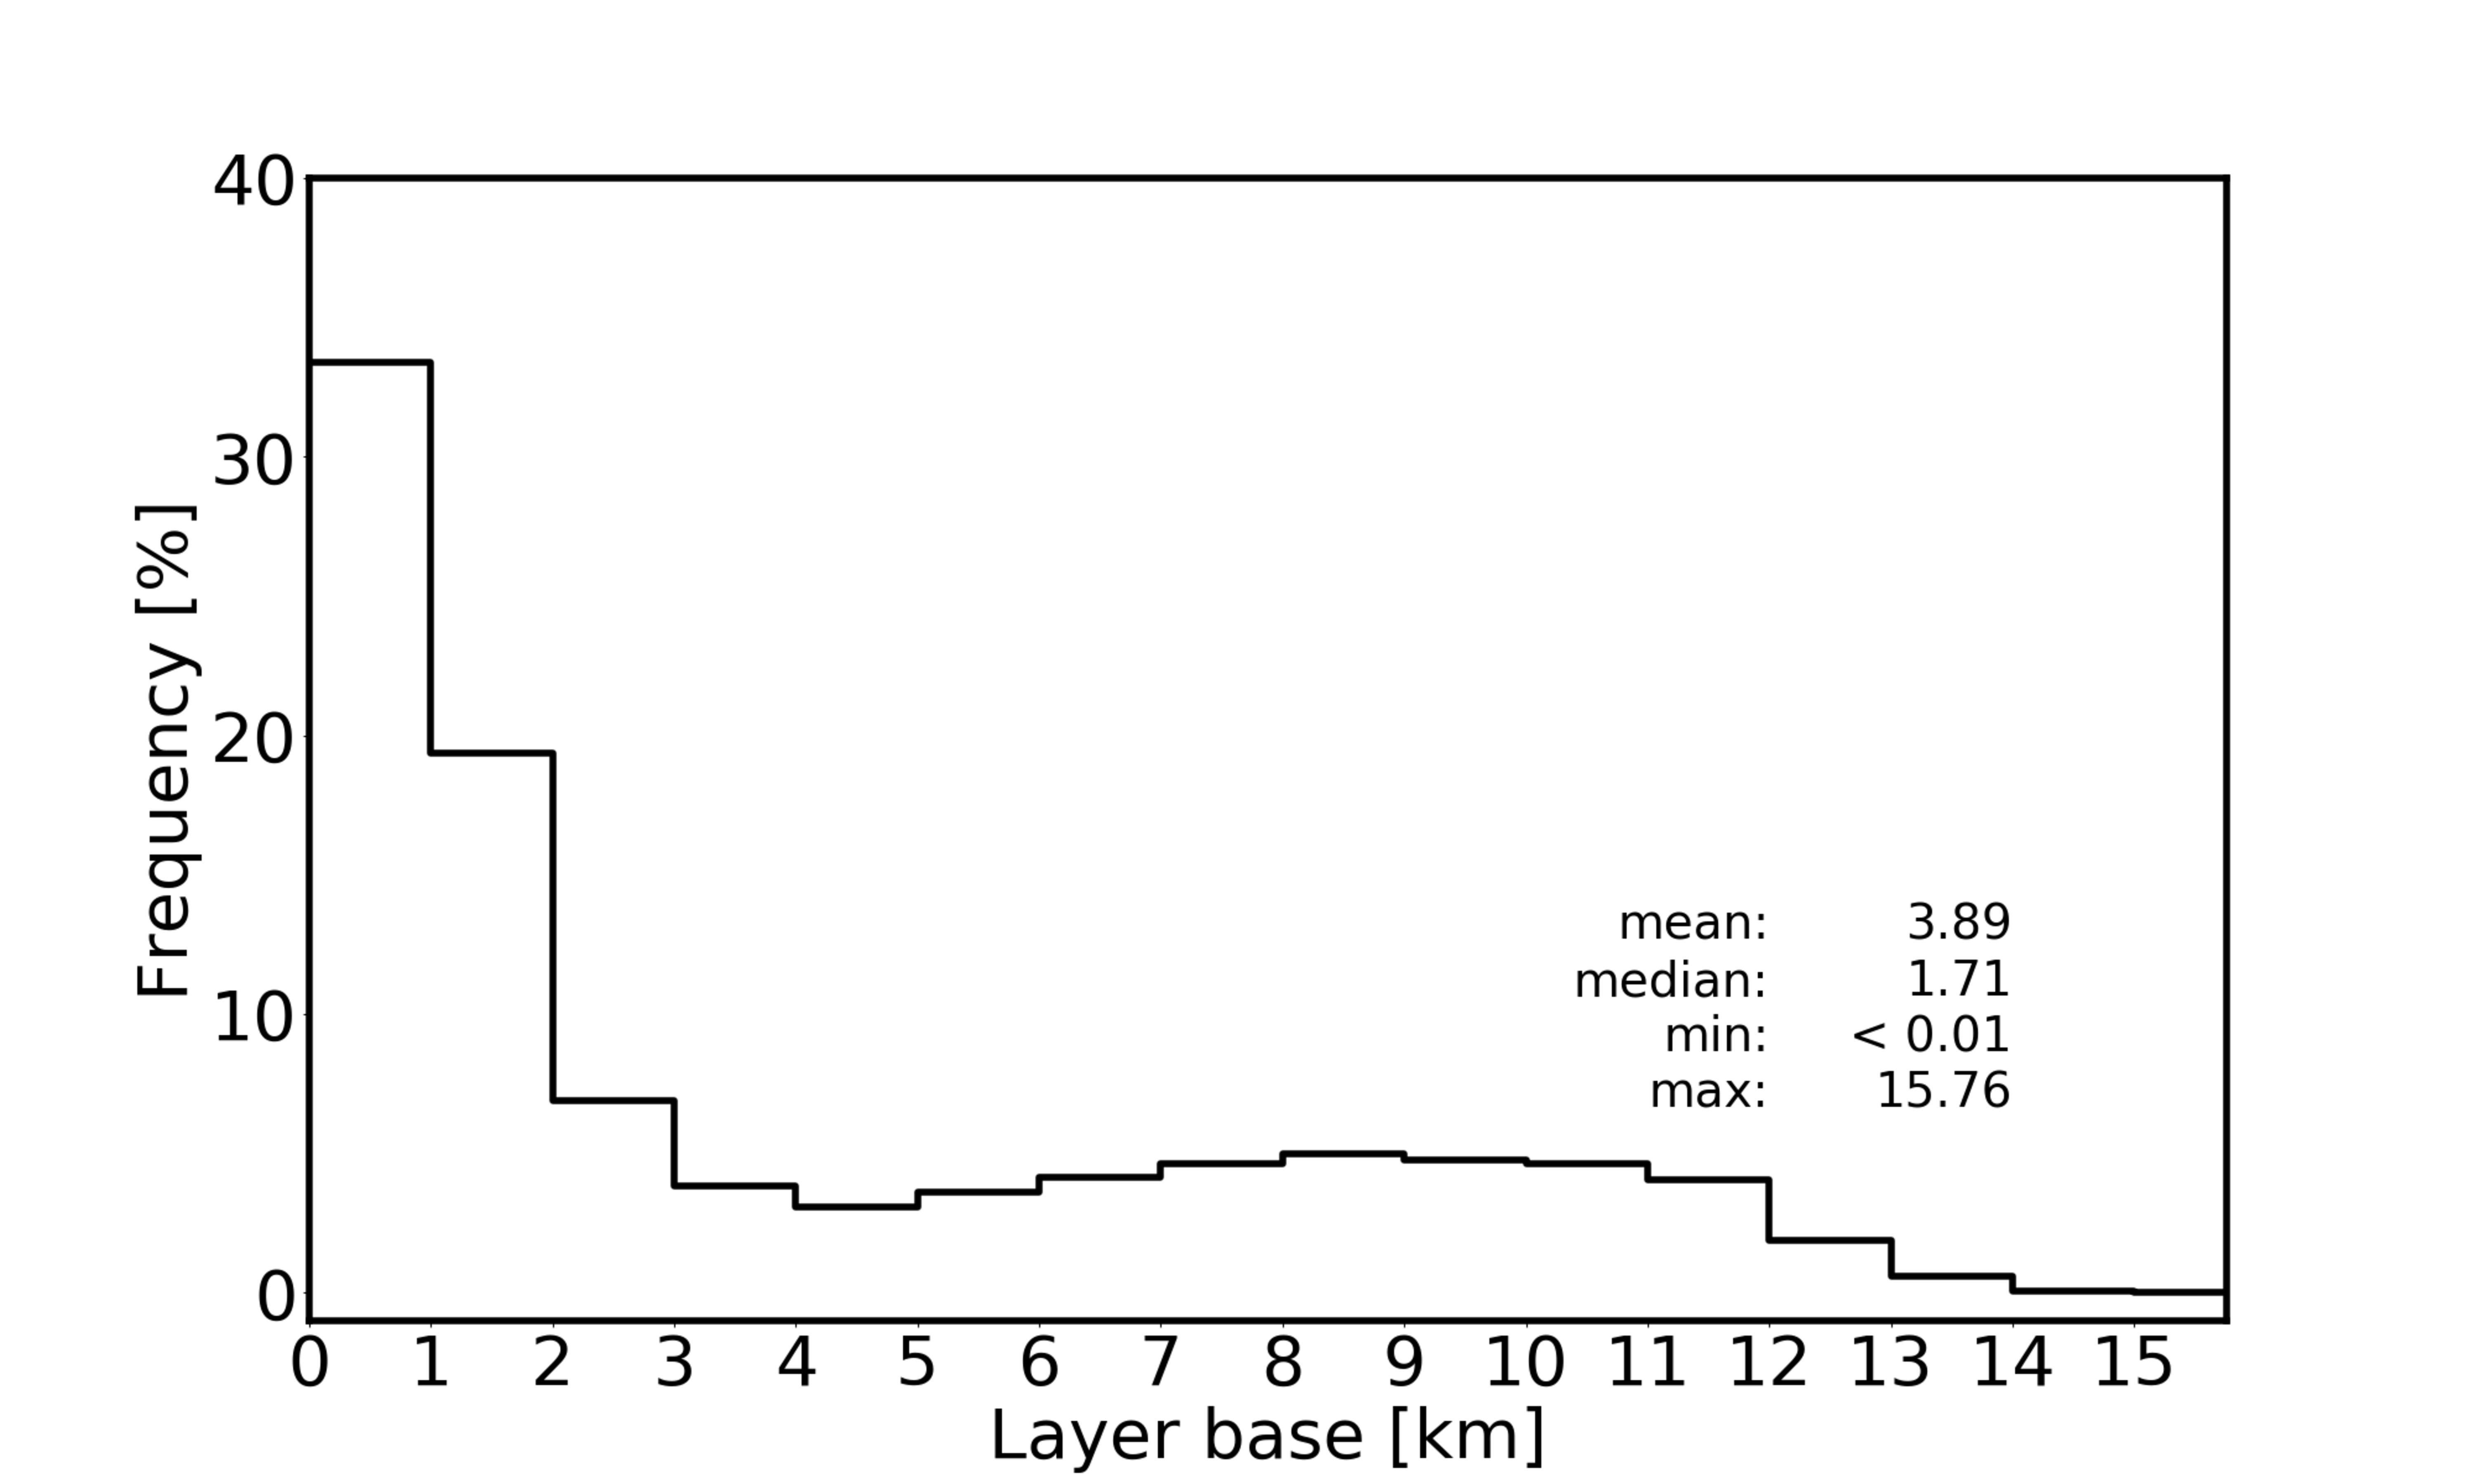
\includegraphics[width=\textwidth]{layerbase_pdf_monsoondomain_monsoonseason.png}
           \label{fig:pdf1}
    \end{subfigure}%
    ~ 
    \begin{subfigure}[b]{0.5\textwidth}
        \centering
        \caption{westerly}        
        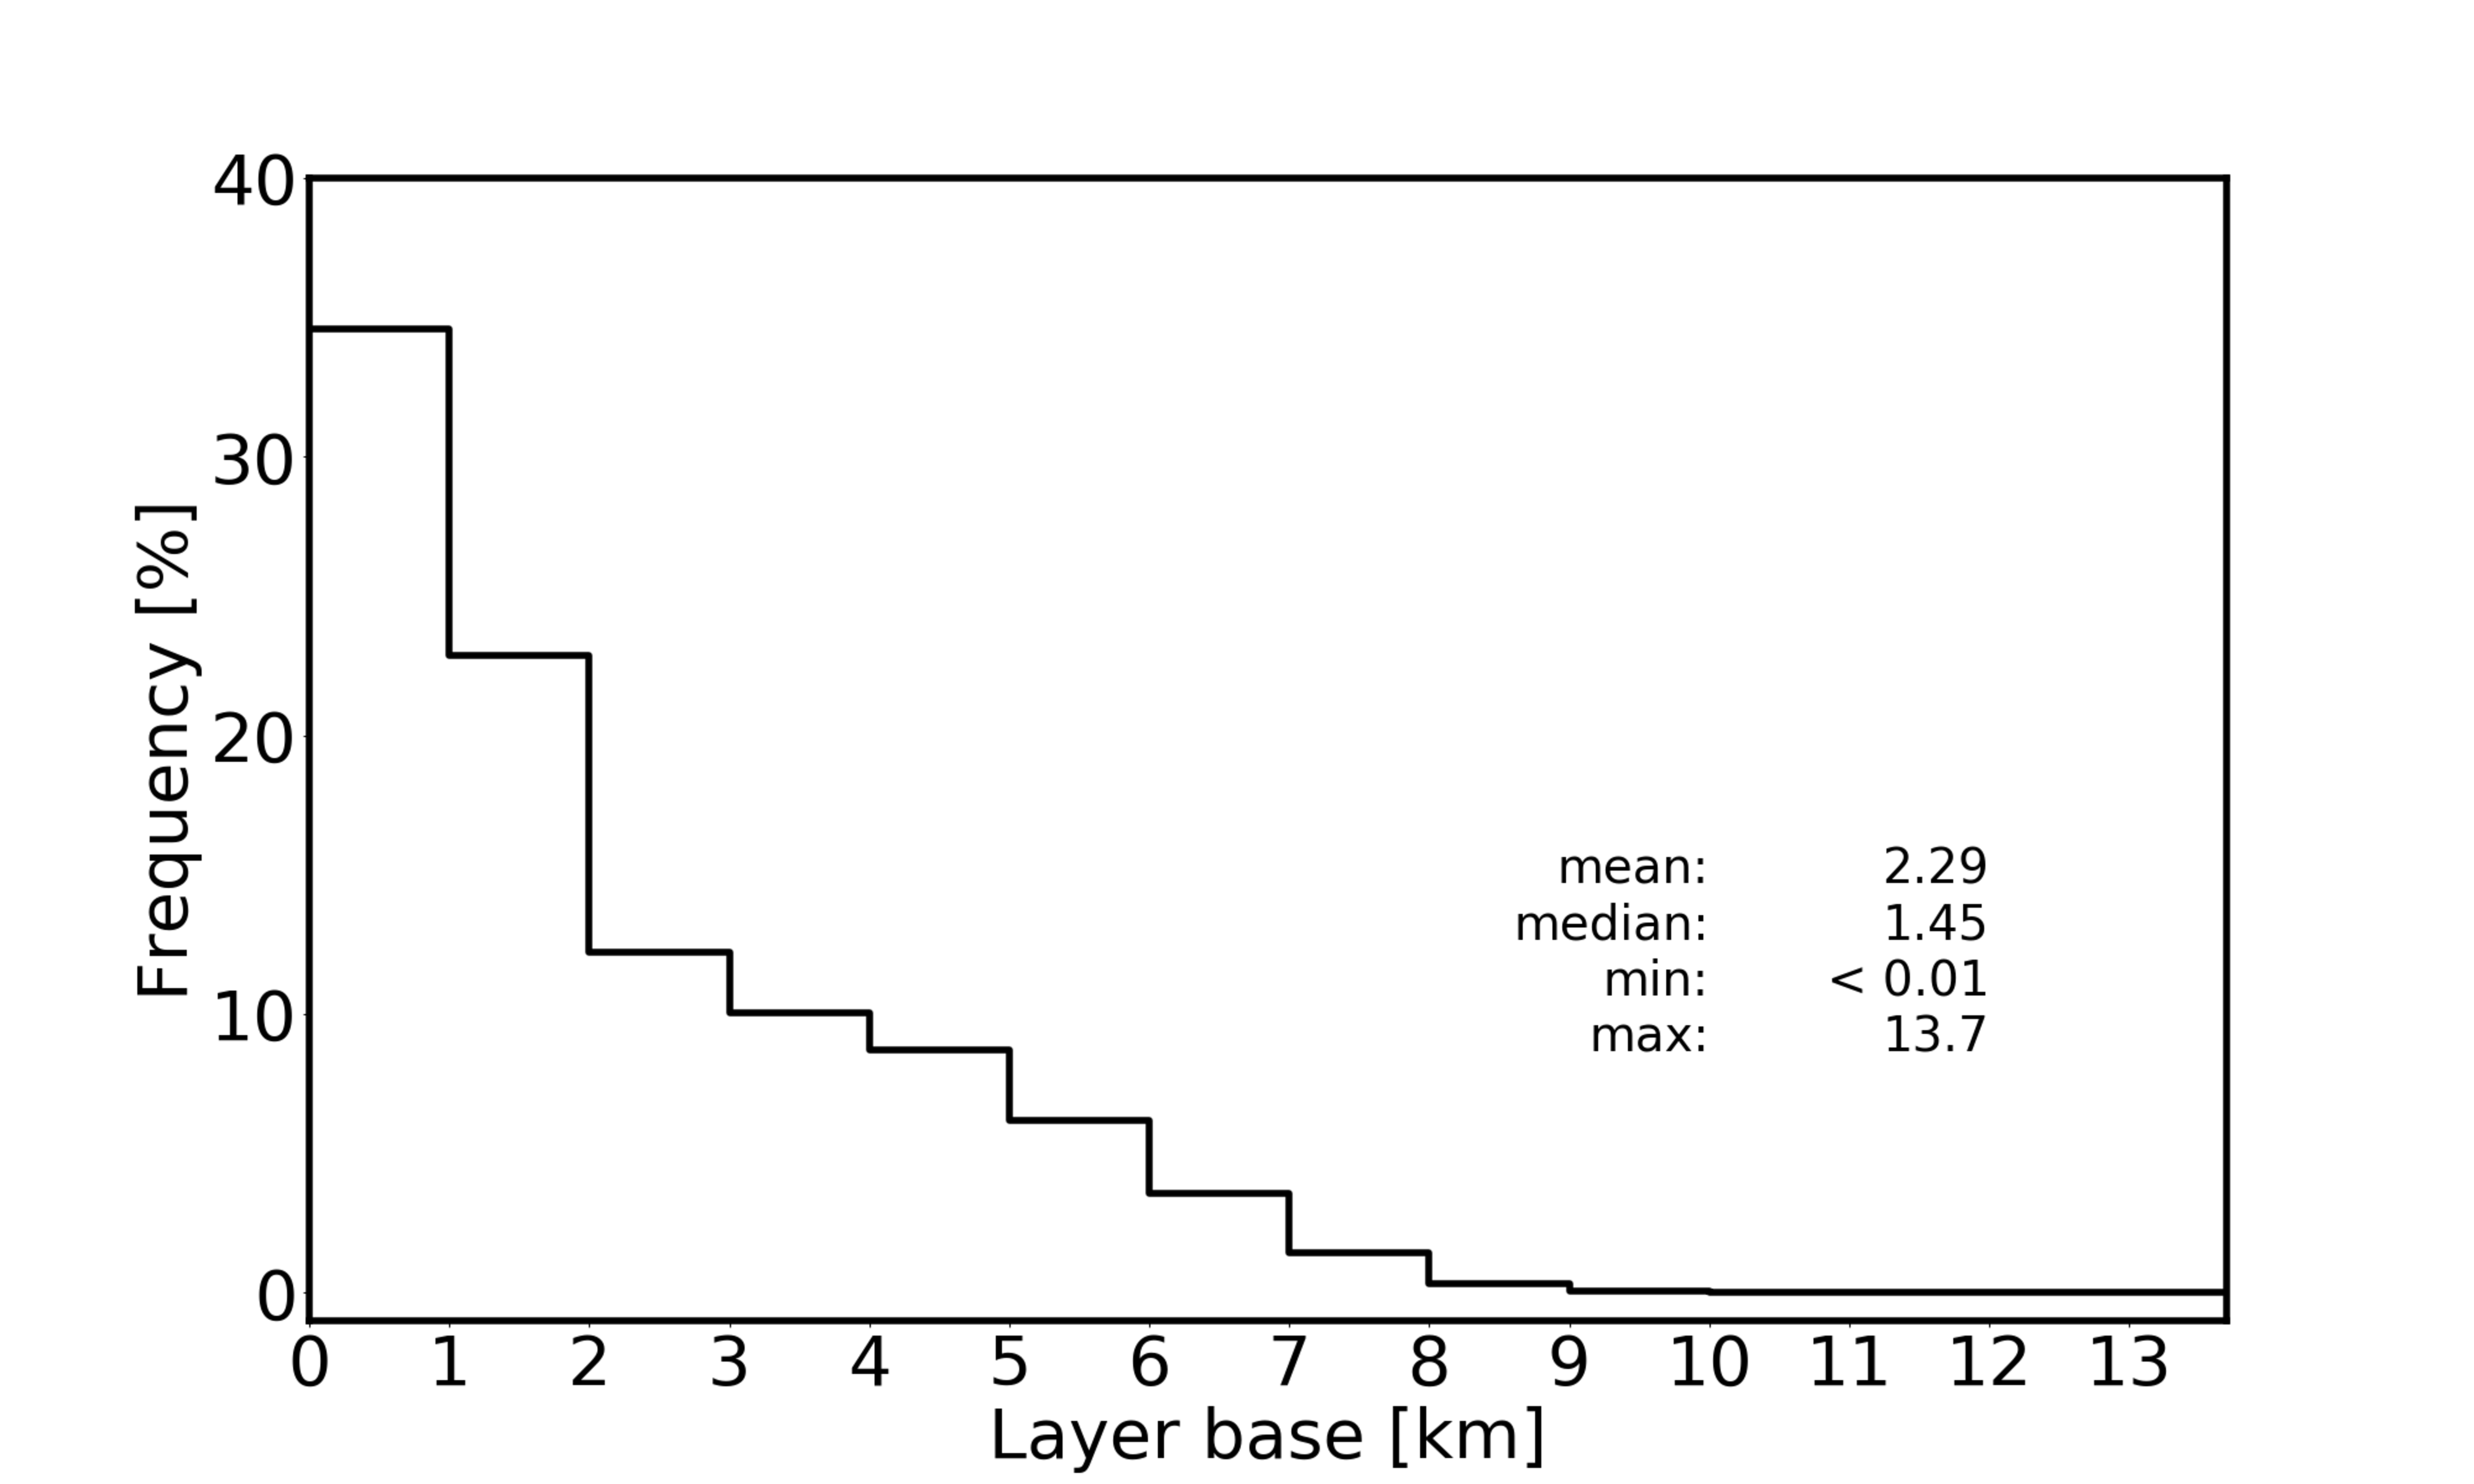
\includegraphics[width=\textwidth]{layerbase_pdf_westerlydomain_westerlyseason.png}
           \label{fig:pdf2}
    \end{subfigure}
    
        \bigskip
        
   \begin{subfigure}[b]{0.5\textwidth}
       \centering
        \caption{monsoon}       
        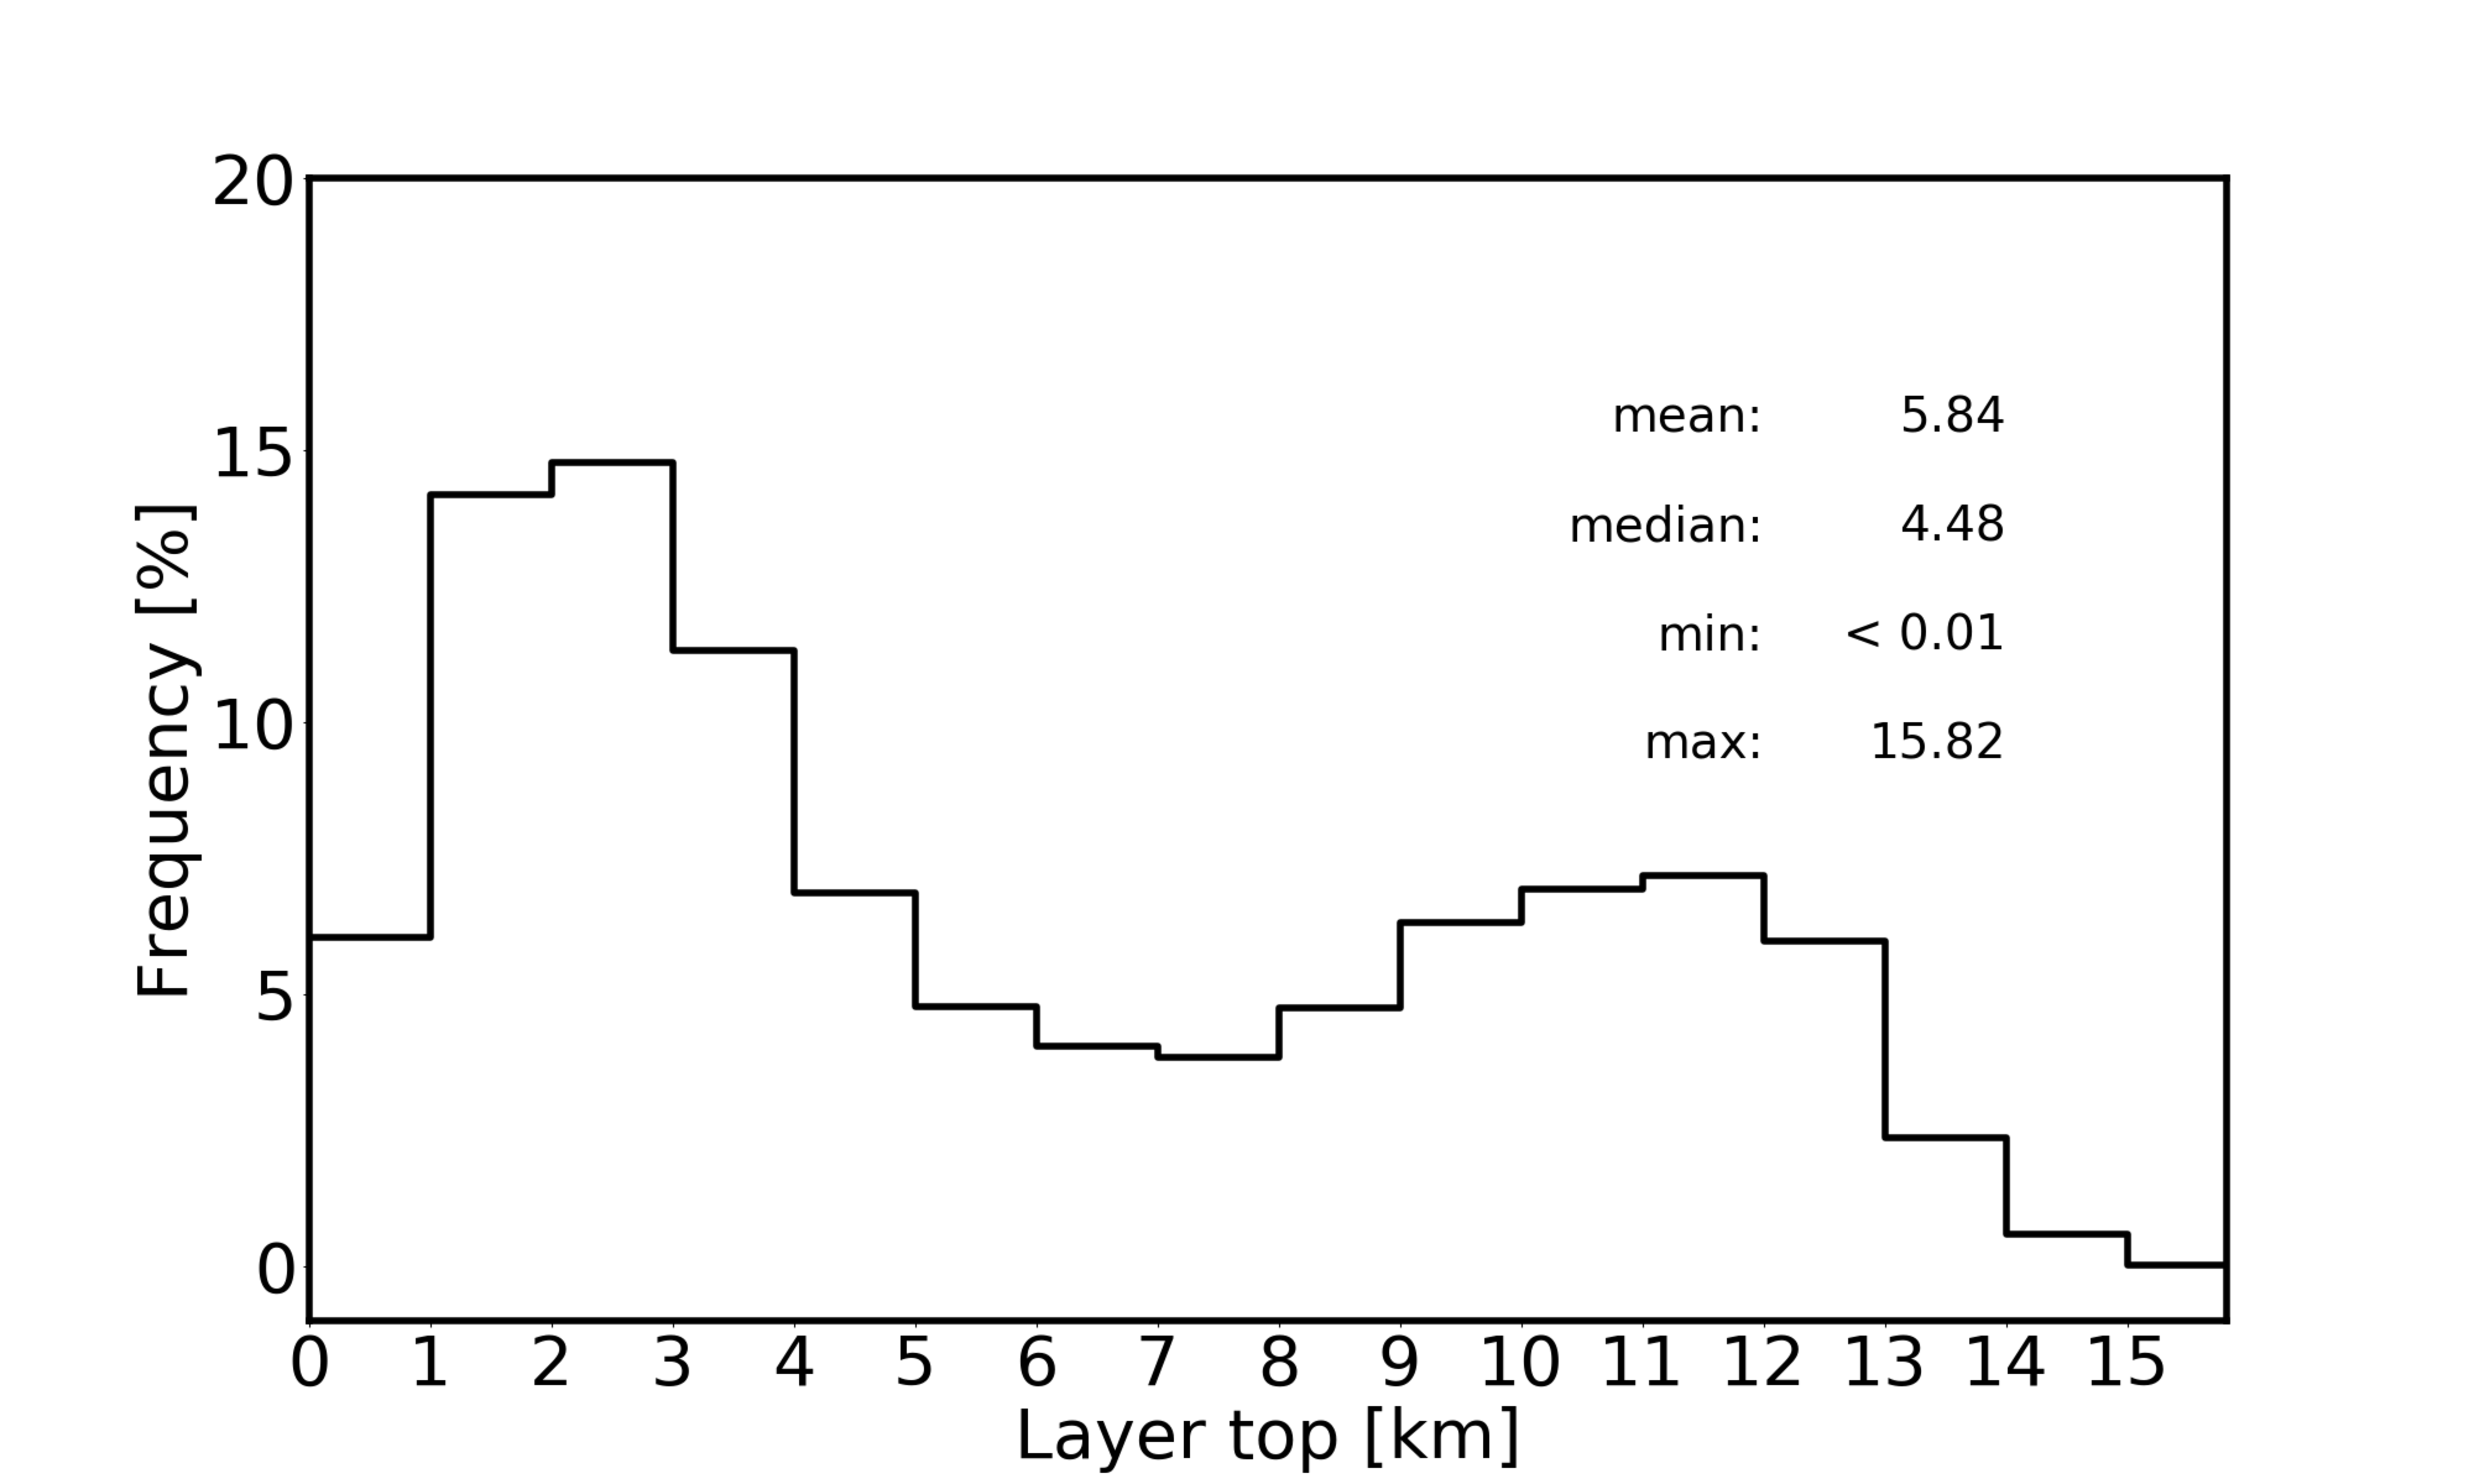
\includegraphics[width=\textwidth]{layertop_pdf_monsoondomain_monsoonseason.png}
   \label{fig:pdf3}
    \end{subfigure}%
    ~ 
    \begin{subfigure}[b]{.5\textwidth}
        \centering
\caption{westerly}        
        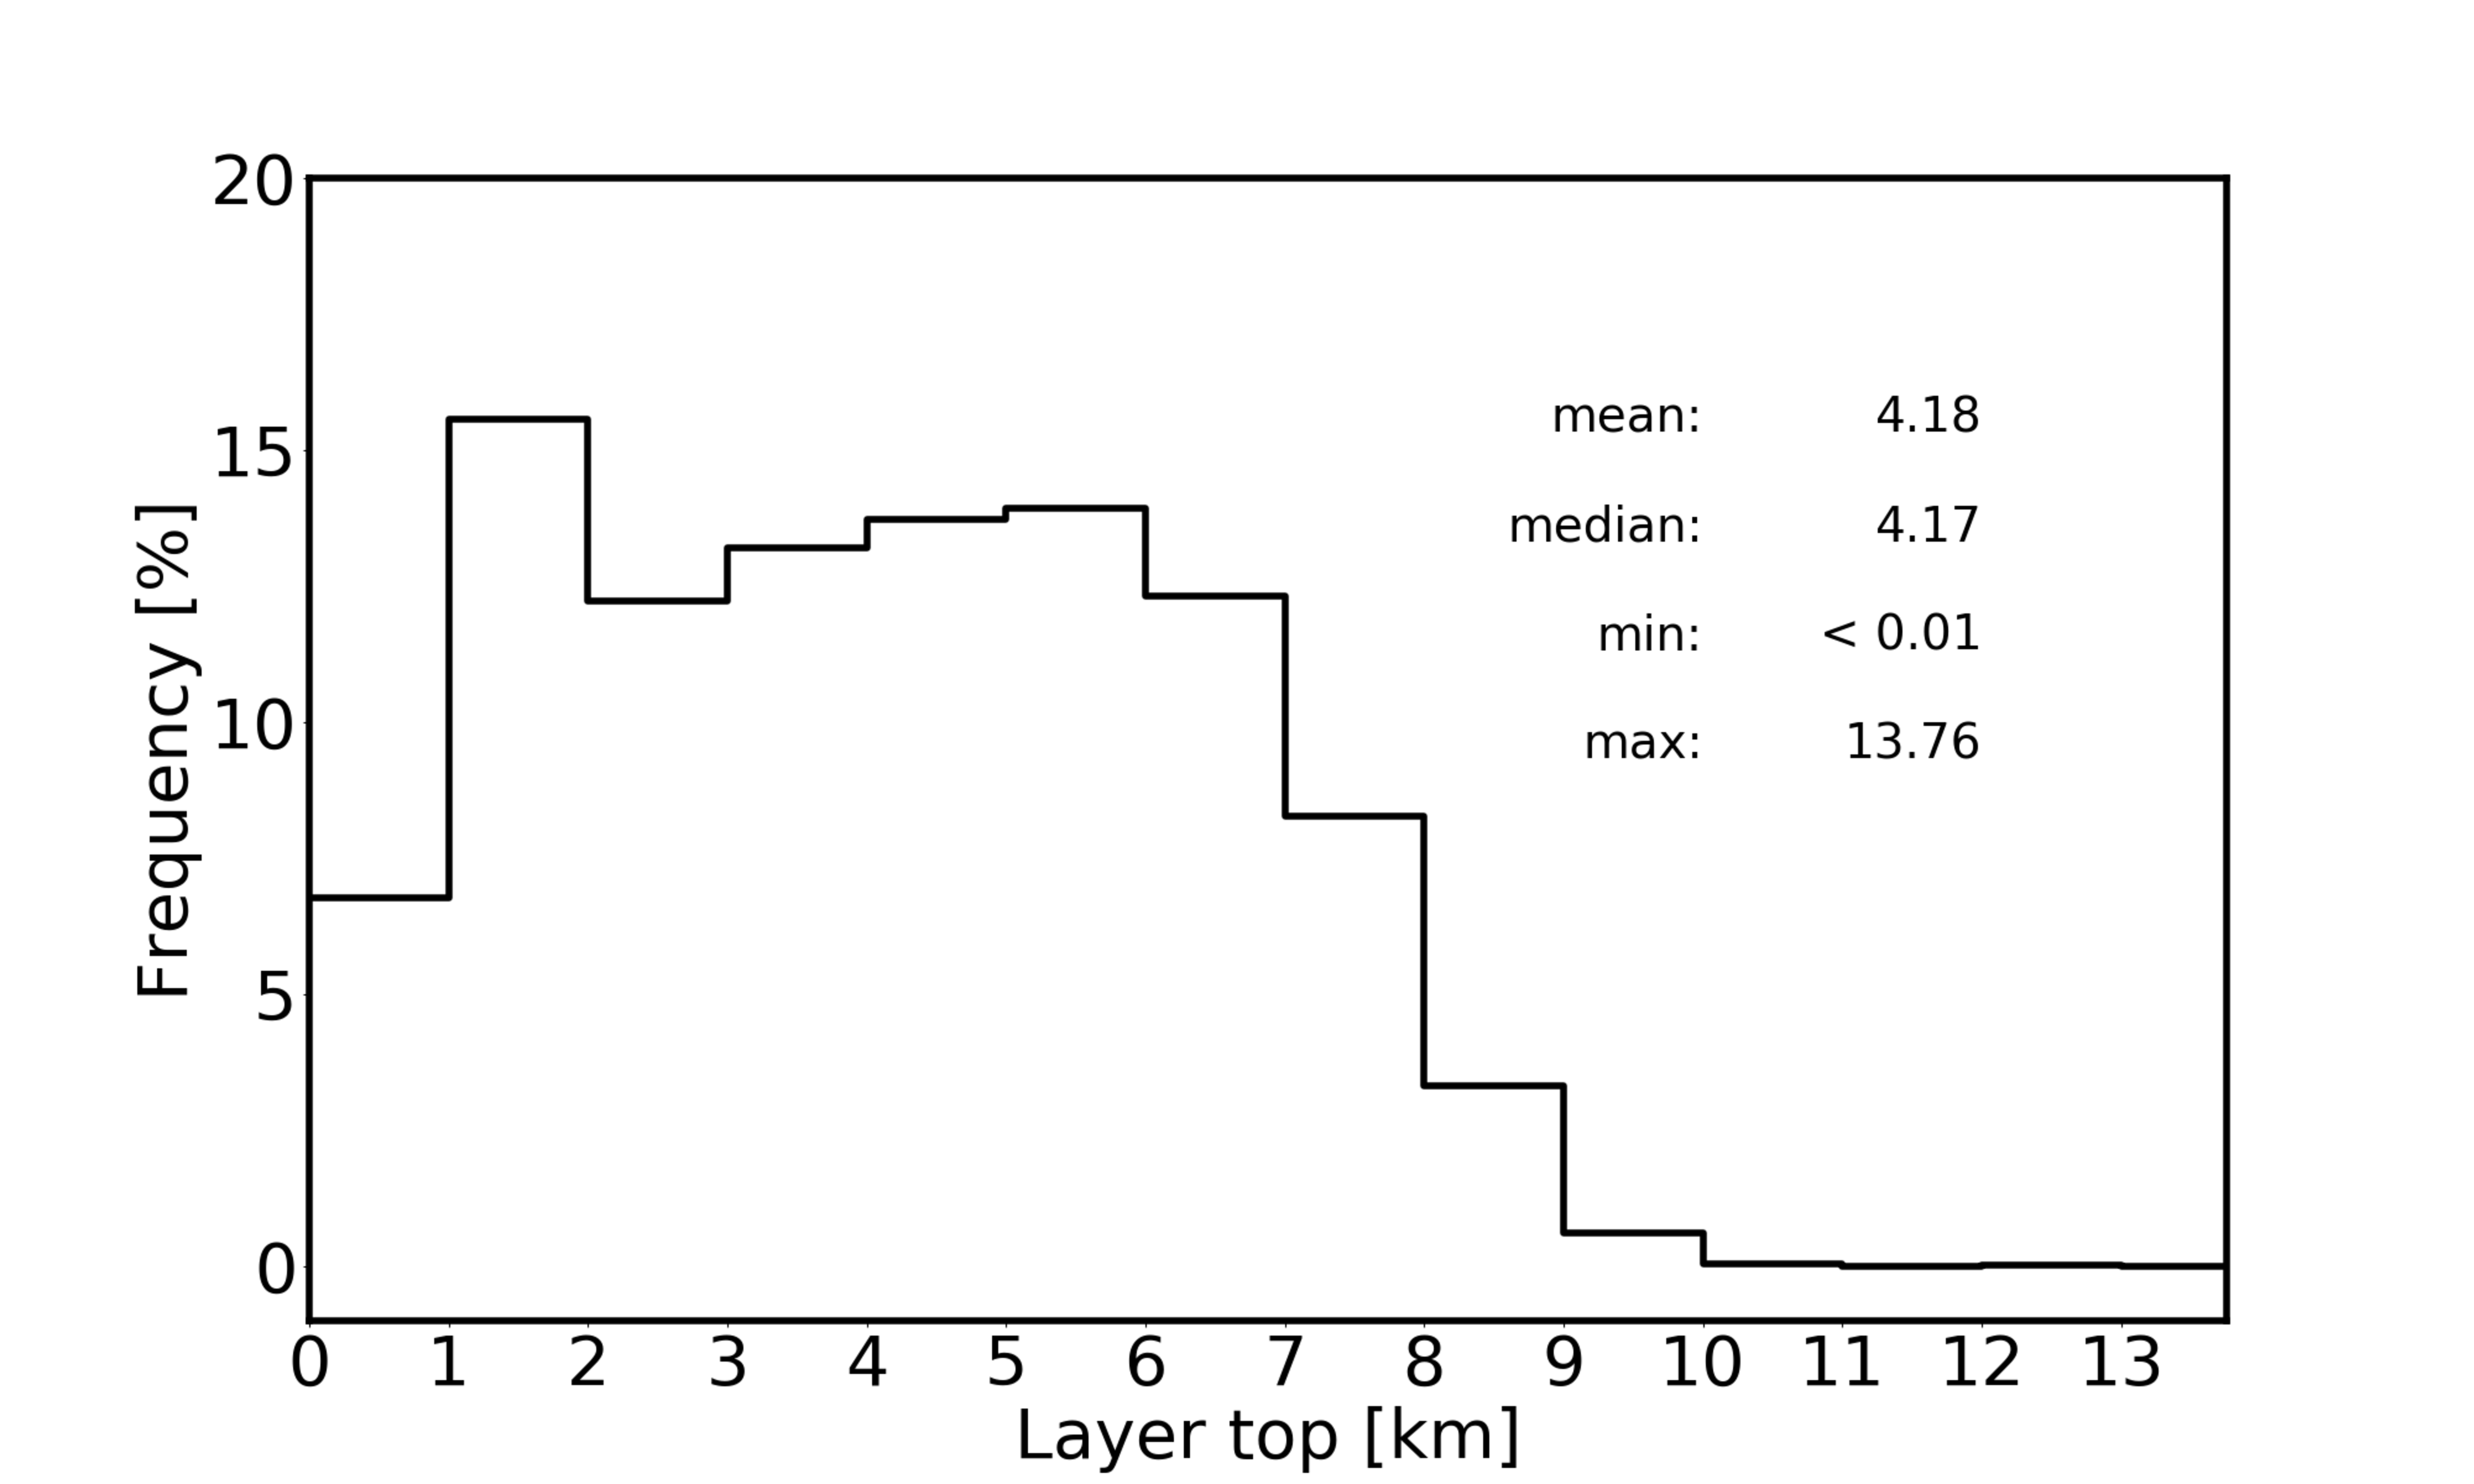
\includegraphics[width=\textwidth]{layertop_pdf_westerlydomain_westerlyseason.png}
   \label{fig:pdf4}
    \end{subfigure}

    \begin{subfigure}[b]{0.5\textwidth}
        \centering
        \caption{monsoon }        
        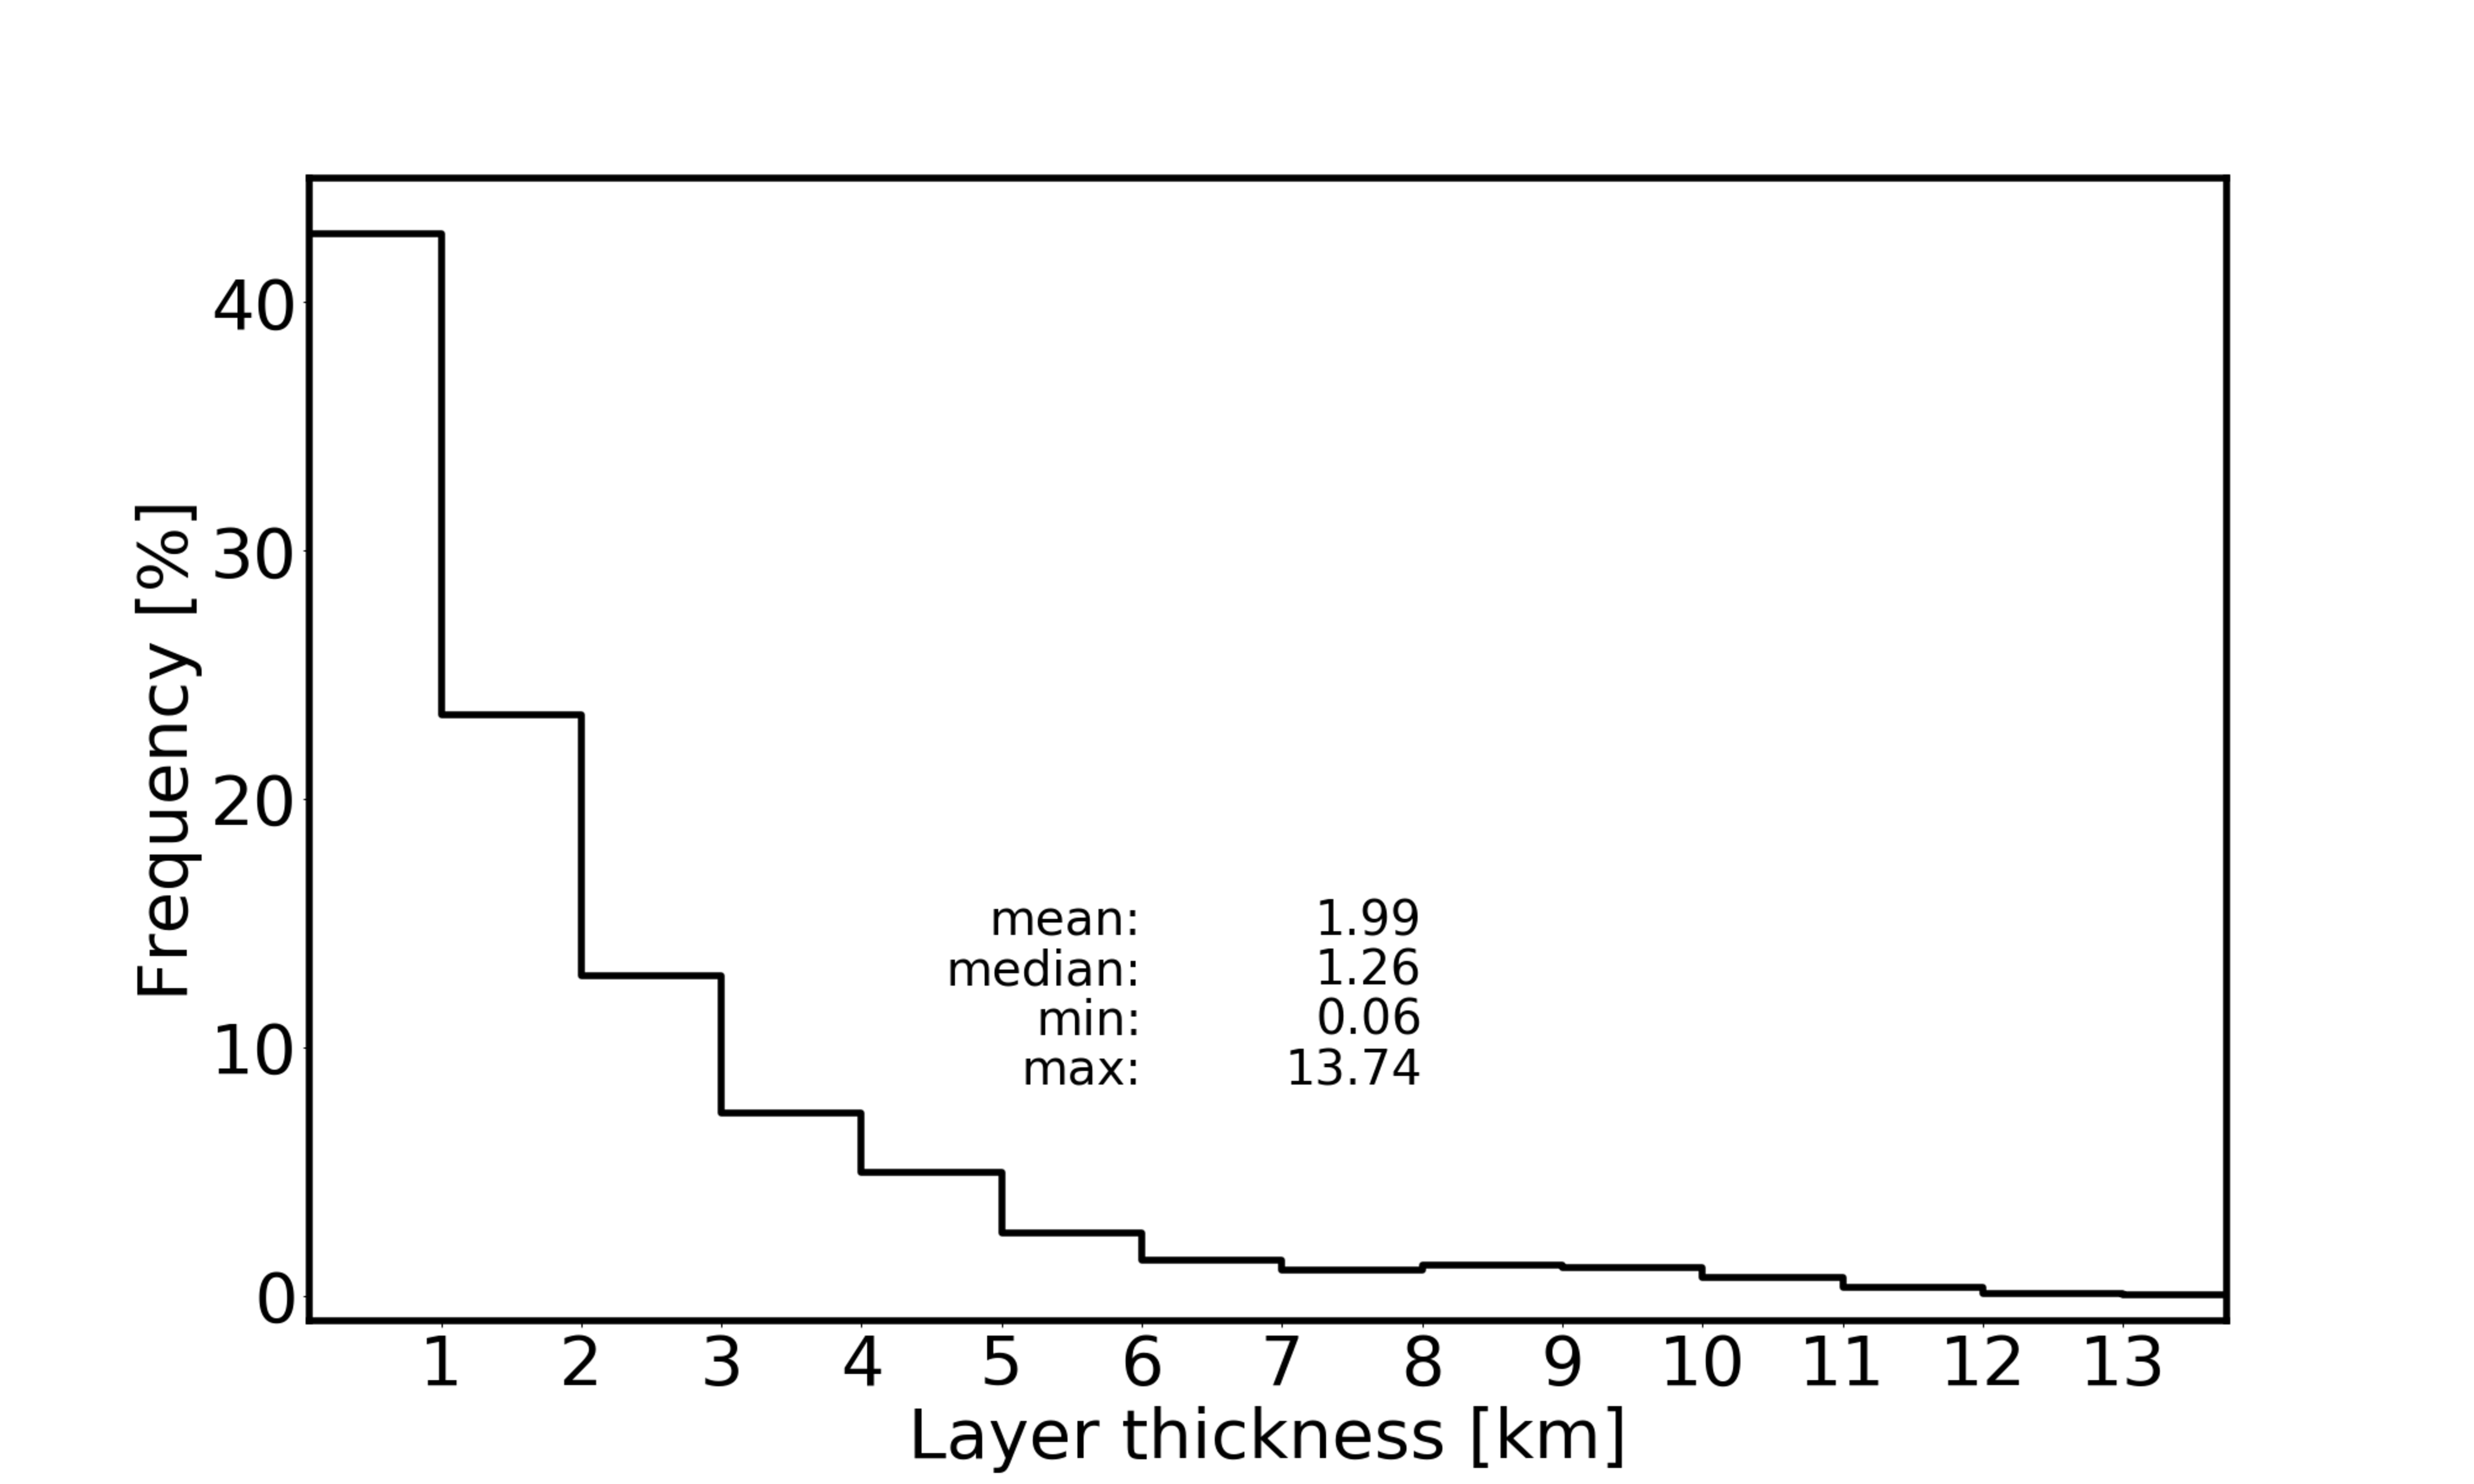
\includegraphics[width=\textwidth]{layerthickness_pdf_monsoondomain_monsoonseason.png}
   \label{fig:pdf5}
    \end{subfigure}%
    ~ 
    \begin{subfigure}[b]{0.5\textwidth}
        \centering
        \caption{westerly}        
        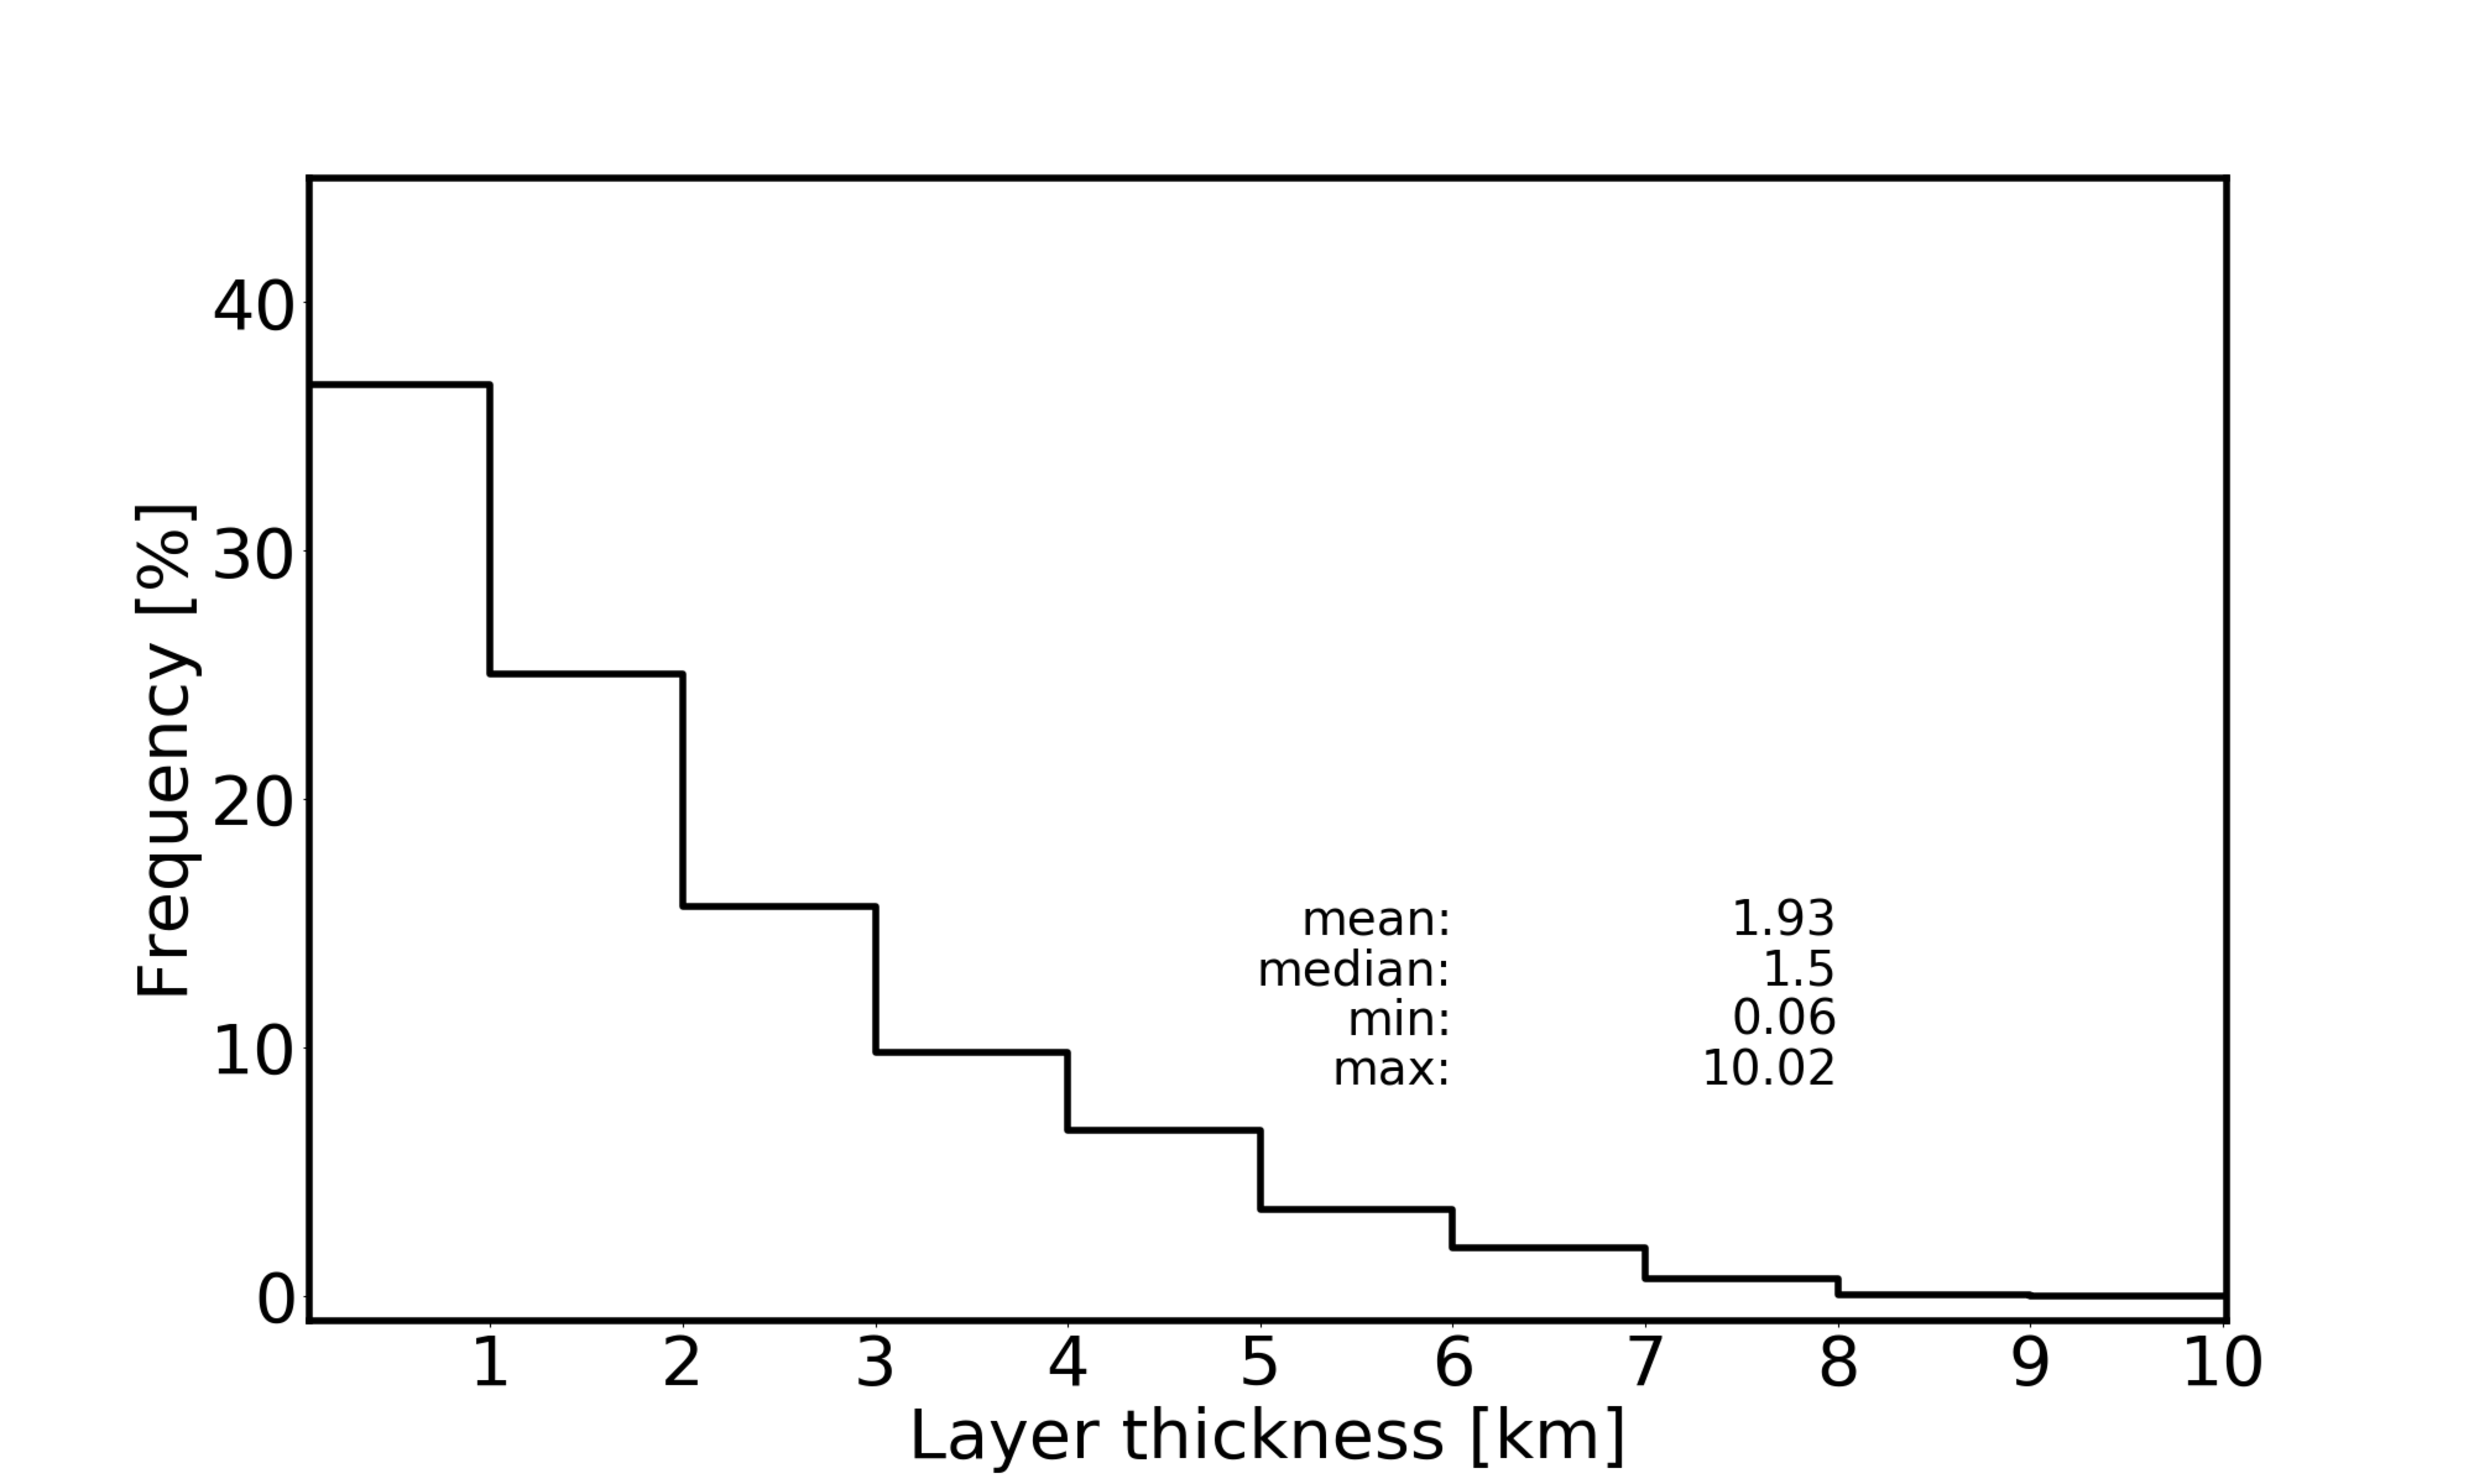
\includegraphics[width=\textwidth]{layerthickness_pdf_westerlydomain_westerlyseason.png}
           \label{fig:pdf6}
        \end{subfigure}
        \caption{PDF of cloud layer base height, top height and thickness (km) for the monsoon-dominated domain during the monsoon season (a, c, e) and for the westerly-dominated domain during the westerly season (b, d, f) based on 2B-CLDCLASS-LIDAR (2007 -- 2010).}
\label{fig:pdf}
\end{figure}  


\subsection{Ice clouds}


As shown in the previous section, cloud layers over the TP show both seasonal and regional variations in vertical structure, which also has implications for its microphysical properties. Figure \ref{fig:monthly_cldphase} shows the monthly variation of cloud particle phase by examining occurrence frequencies of ice, mixed-phase and liquid cloud layers over the TP and in the three subregions. Whereas more than 50 \% of cloud layers over the TP are ice clouds during the entire year, its contribution exceeds 80 \% between January and April (Fig. \ref{fig:monthly_cldphase1}). This shows clearly that ice cloud layers are the most frequent cloud phase type over the plateau, despite the seasonal and regional variations. 

Liquid clouds peak between June and August in the westerly-dominated domain and the transition zone (Fig. \ref{fig:monthly_cldphase3}, \ref{fig:monthly_cldphase4}) and are most frequent in the monsoon-dominated domain, where more than 50 \% of the cloud layers are liquid clouds in October (Fig. \ref{fig:monthly_cldphase2}). This result reflects also the higher occurrence of convective cloud types in the monsoon-dominated domain during the monsoon season (Fig. \ref{fig:cld_type3}), since the liquid water content is generally higher for convective clouds. The monsoon season and the chosen monsoon-dominated domain of the TP point thus towards distinct signals in cloud characteristics with higher contributions of convective cloud types and lower contributions of ice clouds. Even though cloud occurrences are higher during the monsoon season and in the monsoon-dominated domain, the relative fractions of the most common cloud characteristics (including stratiform, ice and single-layer cloud layers) decrease, which means that hydrometeor sizes, cloud types and cloud macrophysical properties depict higher variations. 

However, high-level cirrus clouds are, in contrast to total ice clouds, more frequent in the monsoon-dominated domain (Fig. \ref{fig:cld_type1}, \ref{fig:cld_type3}, \ref{fig:cld_type5}), which means that the ice clouds in the westerly-dominated domain might occur at lower levels.  

Moreover, the relative frequencies of ice, mixed-phase and liquid clouds in the subregions highlight the recurring characteristic of the transition zone showing more similar patterns to the westerly-dominated domain than to the monsoon-dominated domain (Fig. \ref{fig:monthly_cldphase3}, \ref{fig:monthly_cldphase4}).


\begin{figure}[!htbp]
\centering
    \begin{subfigure}[b]{0.5\textwidth}
       \centering
        \caption{TP}       
        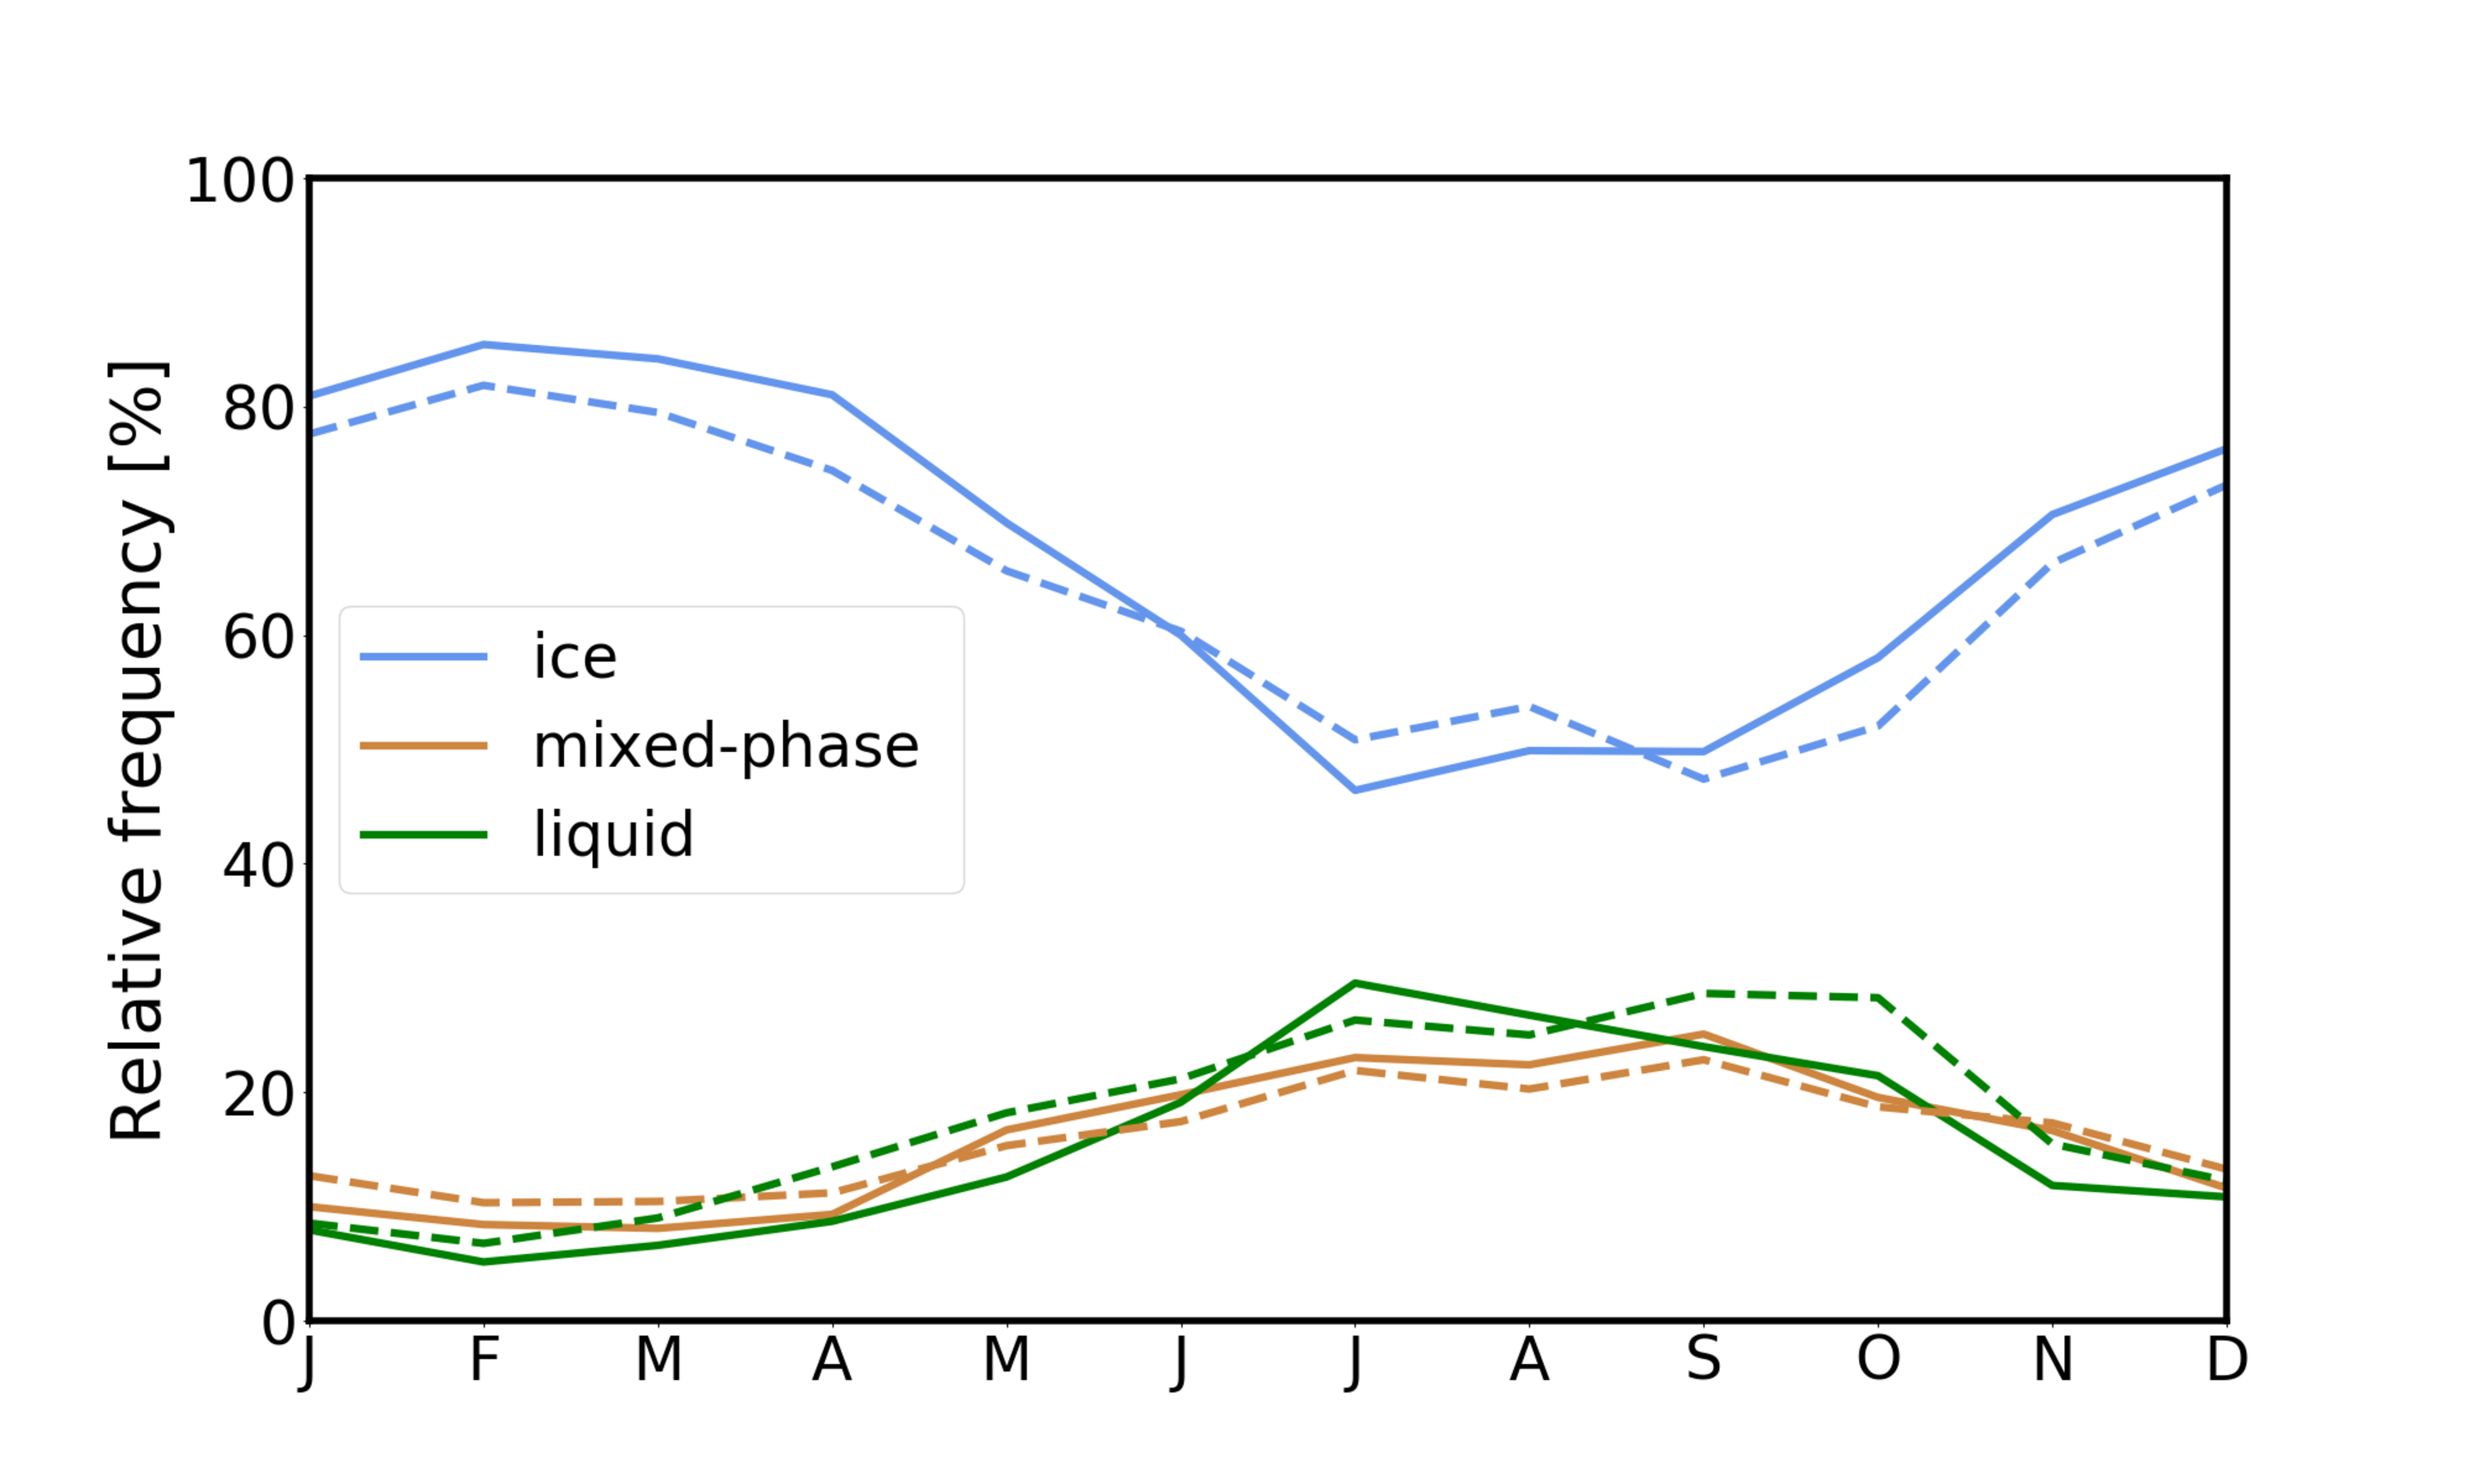
\includegraphics[height=1.5in]{monthly_cldphase_TP.png}
          \label{fig:monthly_cldphase1}
    \end{subfigure}%
    ~ 
    \begin{subfigure}[b]{0.5\textwidth}
        \centering
        \caption{monsoon-dominated} 
        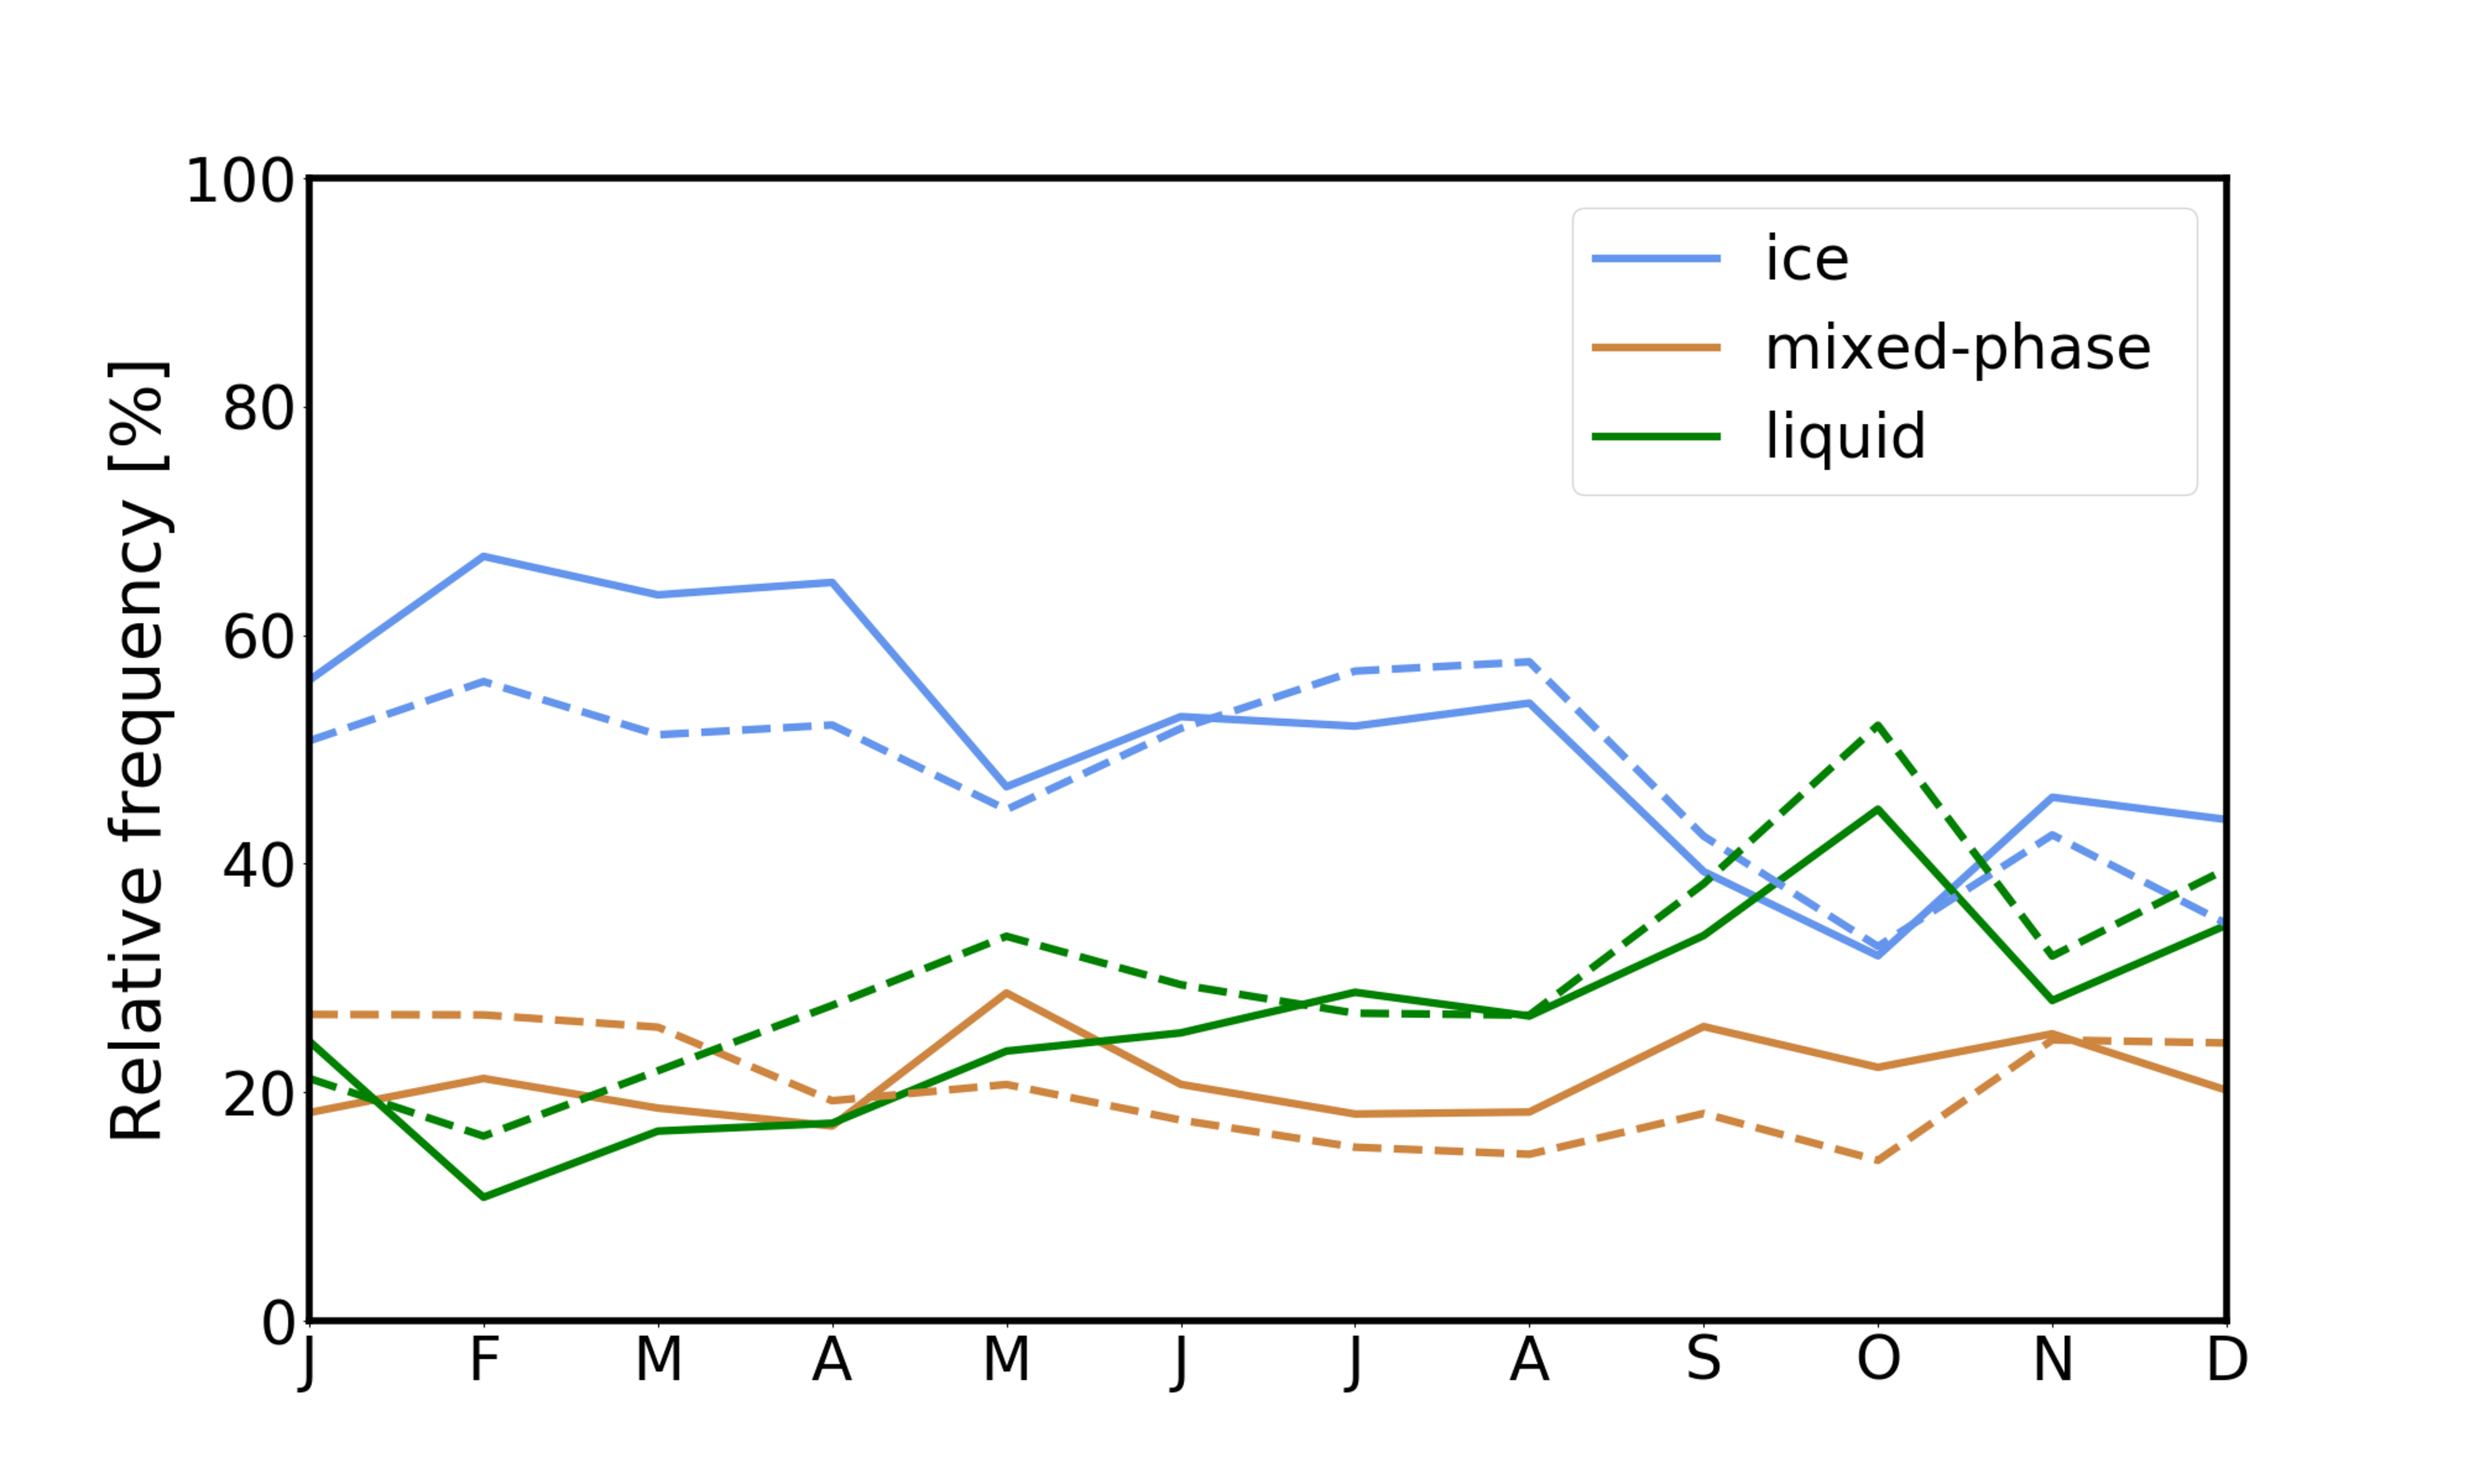
\includegraphics[height=1.5in]{monthly_cldphase_monsoonmode.png}
  \label{fig:monthly_cldphase2}
    \end{subfigure}
    
    \bigskip

    \begin{subfigure}[b]{0.5\textwidth}
        \centering
        \caption{westerly-dominated}        
        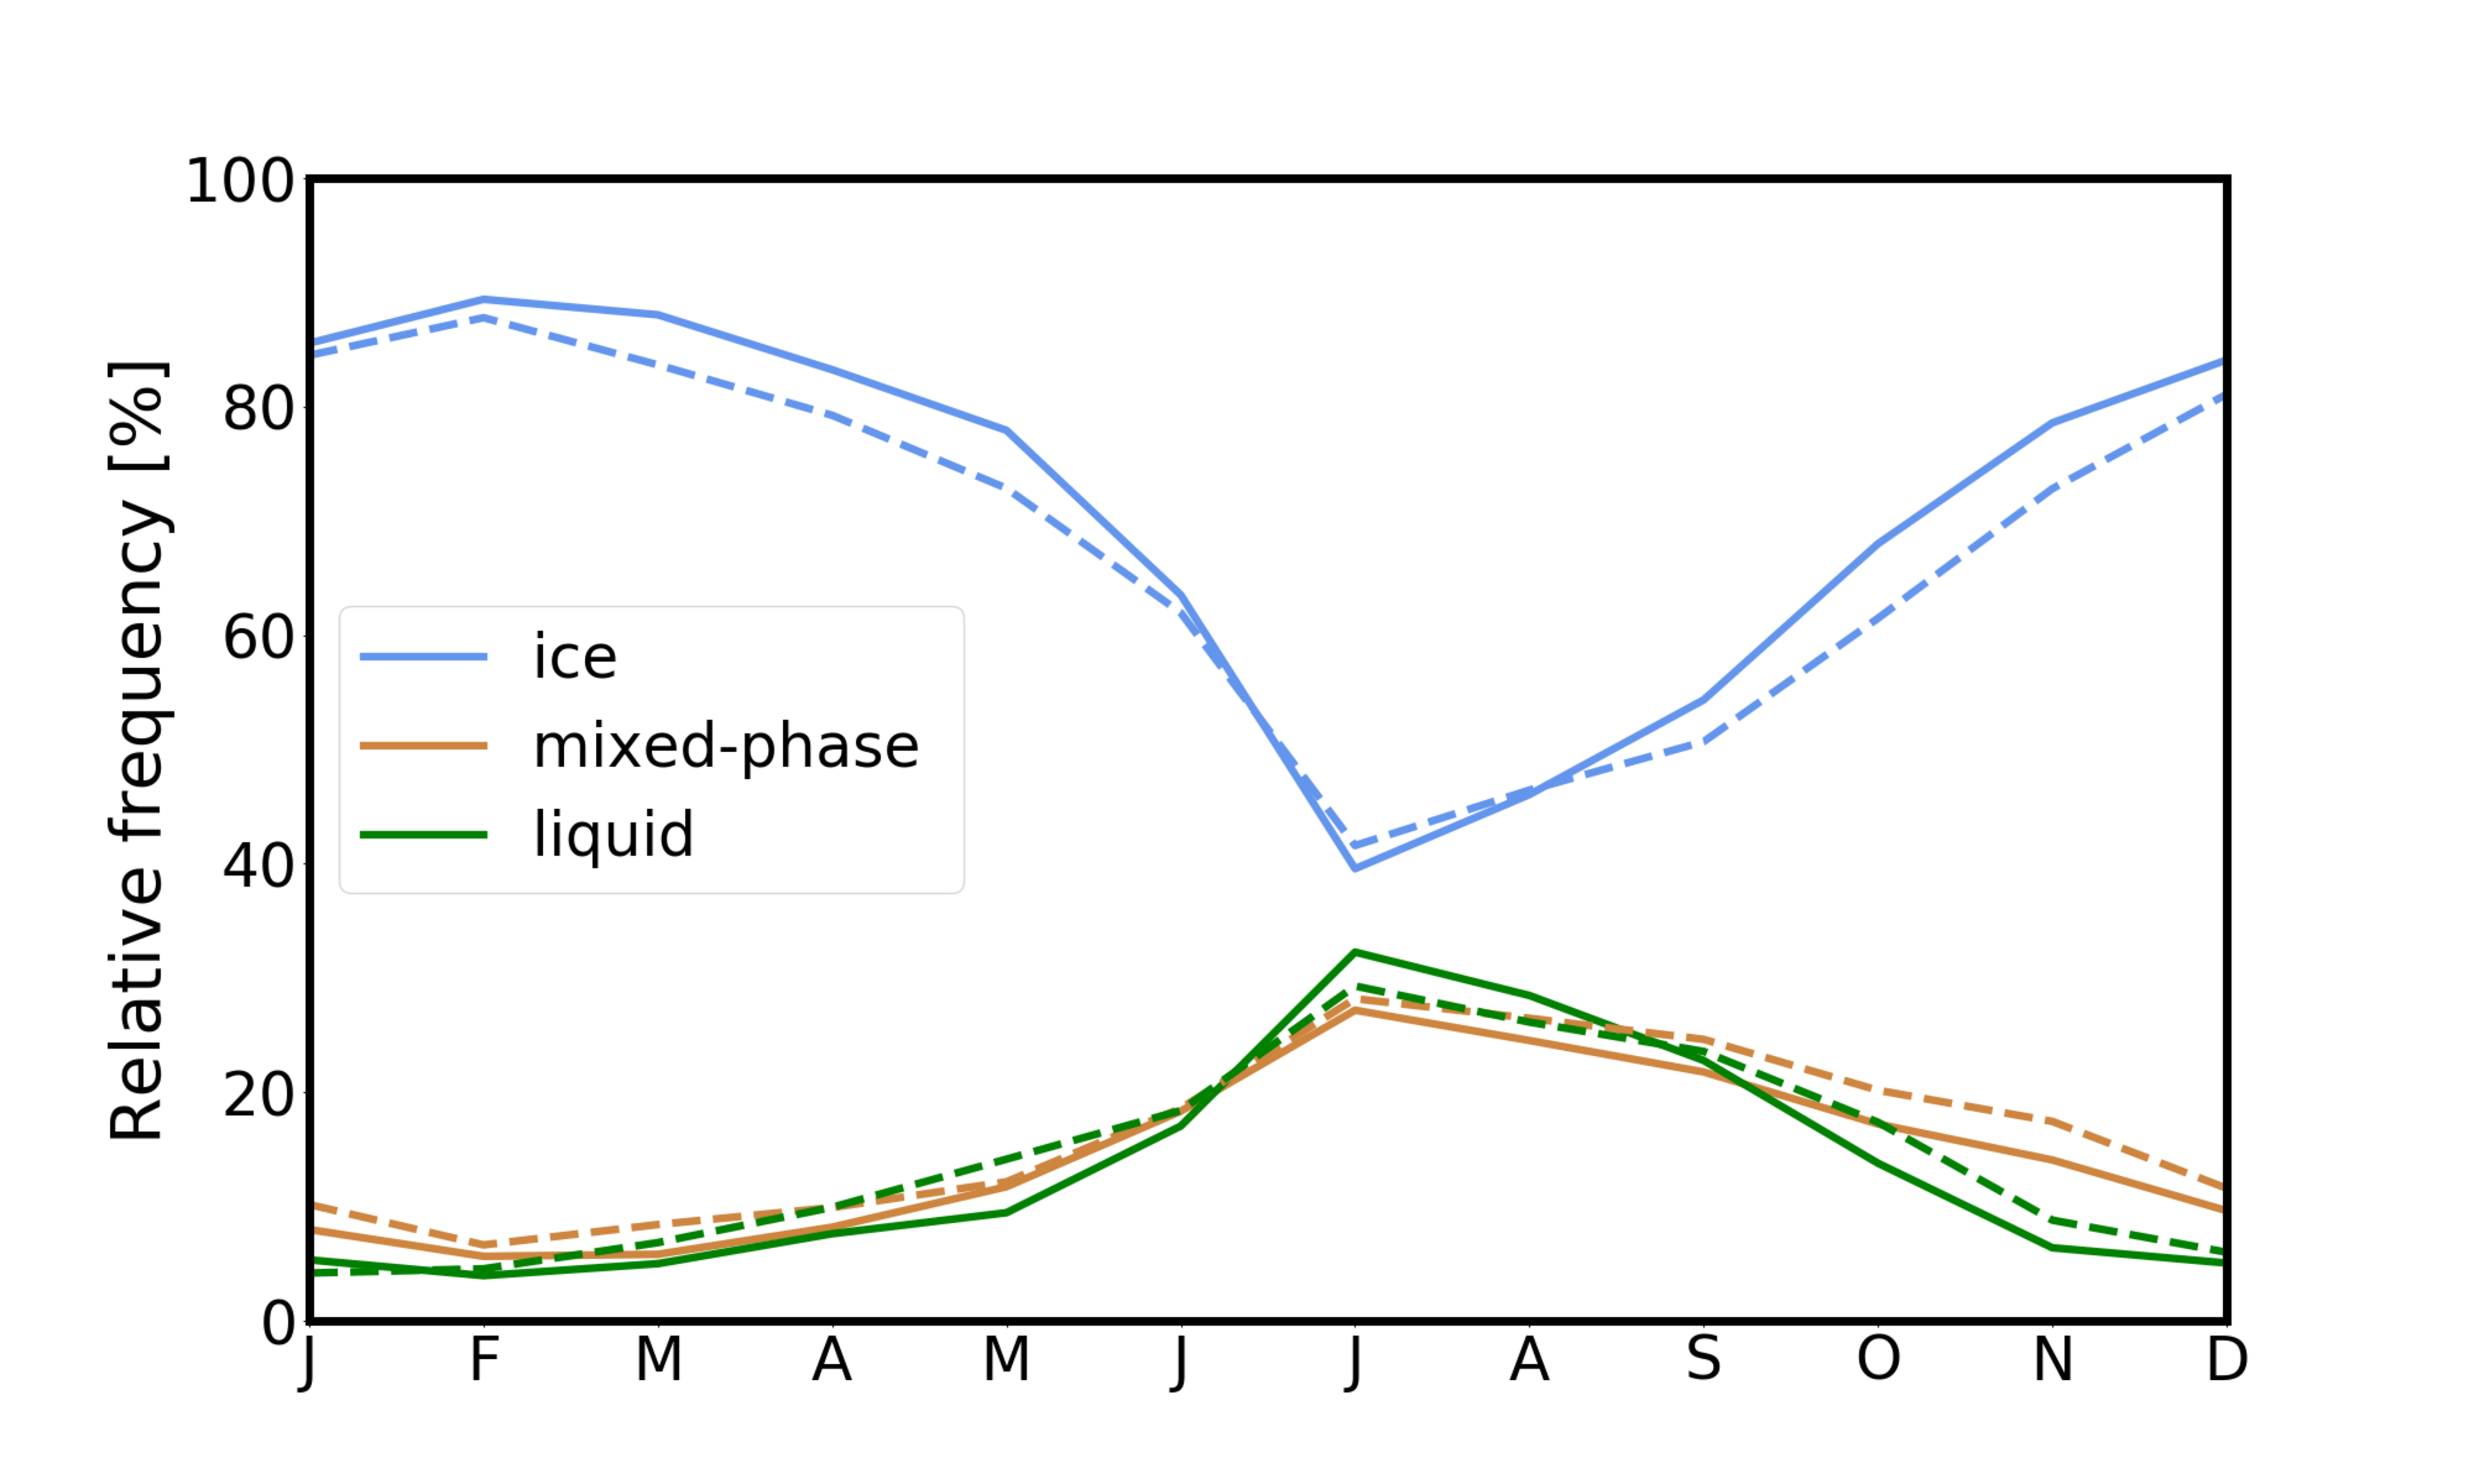
\includegraphics[height=1.5in]{monthly_cldphase_westerlymode.png}
  \label{fig:monthly_cldphase3}
    \end{subfigure}%
        ~ 
    \begin{subfigure}[b]{0.5\textwidth}
        \centering
        \caption{transition zone } 
        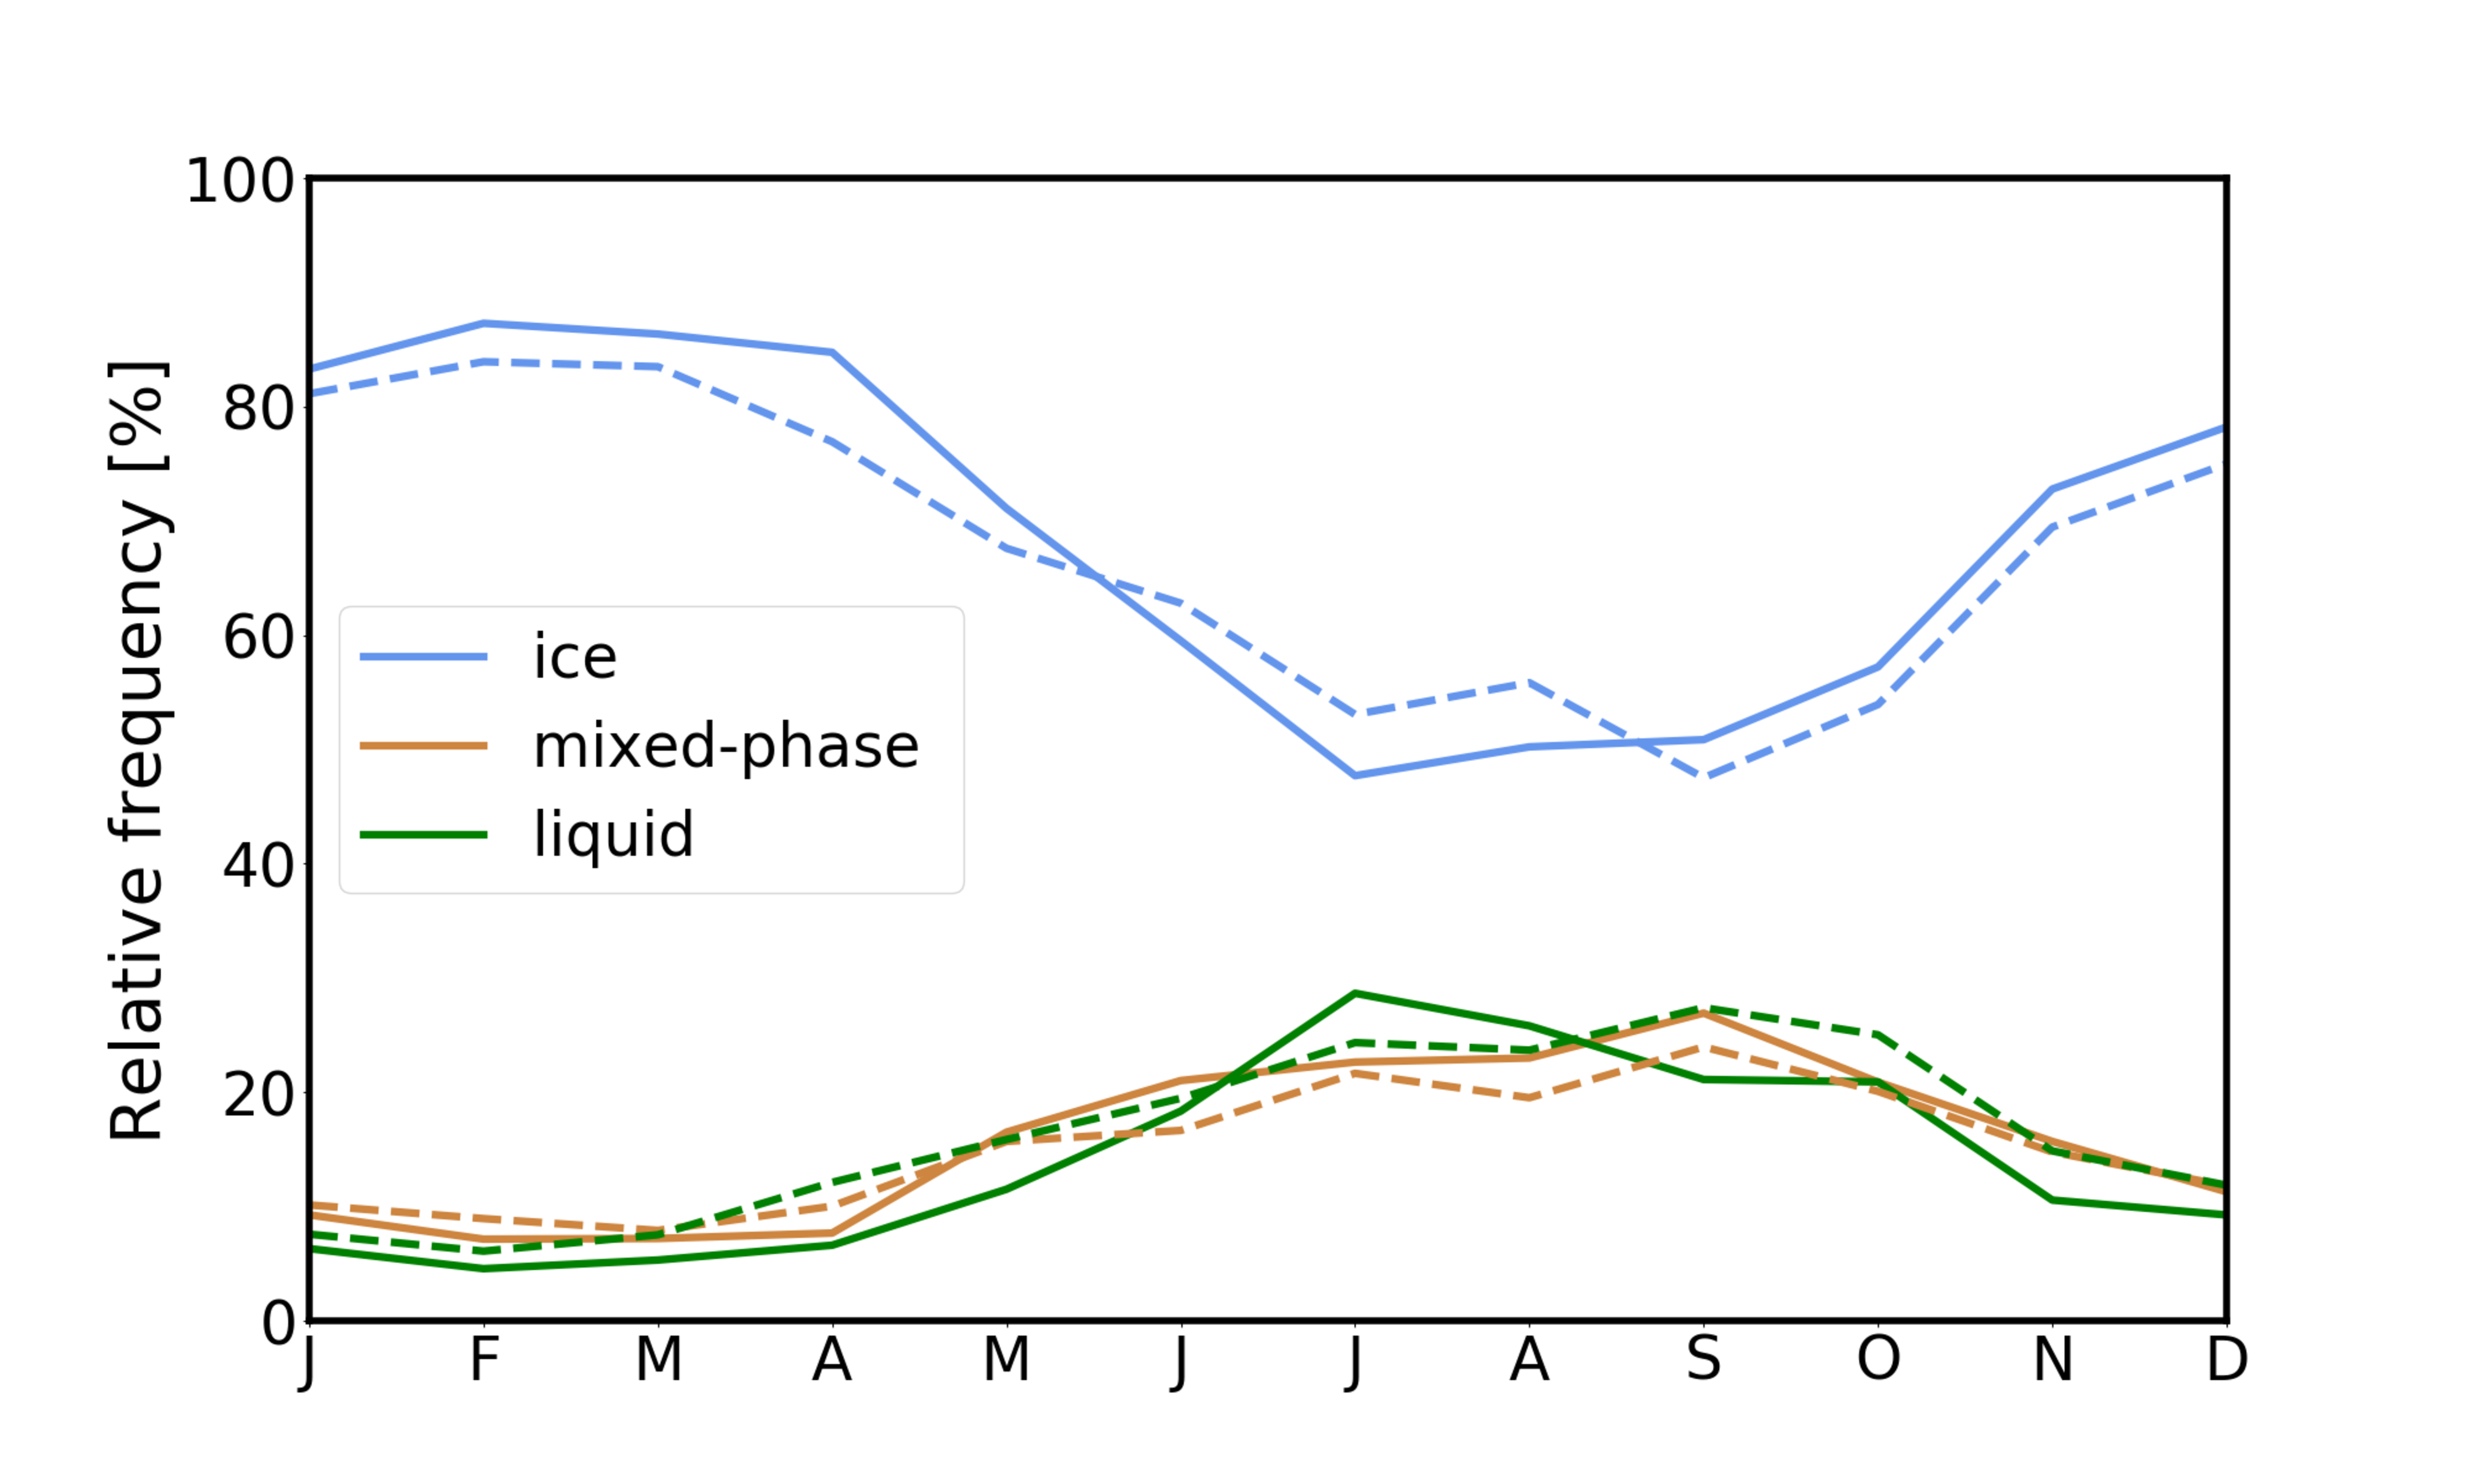
\includegraphics[height=1.5in]{monthly_cldphase_transitionzone.png}
  \label{fig:monthly_cldphase4}
    \end{subfigure}
    \caption{Monthly occurrence frequencies (%) of ice, liquid and mixed-phase cloud layers
for the TP domain (a), monsoon-dominated domain (b), westerly-dominated domain (c)
and transition zone (d) based on 2B-CLDCLASS-LIDAR (2007– 2010). The dashed line
indicates the occurrence frequency of the respective cloud phase types during nighttime
while the solid line describes the occurrence frequency of the cloud phase types during
daytime.}
    \label{fig:monthly_cldphase}
\end{figure}

Figure \ref{fig:od} displays average optical depth values during the monsoon vs. the westerly season for all profiles (Fig. \ref{fig:od1} -- \ref{fig:od2}) , profiles with cloud layer detections (Fig. \ref{fig:od3} -- \ref{fig:od4}) and profiles with liquid cloud layers (Fig. \ref{fig:od5} -- \ref{fig:od6}). While more than half of the optical depth values in the samples of the TP domain are between 0 and 1, its maximum values are above 300 for liquid cloud layers. Fig. \ref{fig:od1} -- \ref{fig:od4} show that the higher mean optical depth values during the monsoon season are also visible when only the optical depth values of the cloudy profiles is taken into account. This indicates that the reason for the higher optical depth values are not only the higher cloud occurrences in general, but also due to the cloud properties. Figure \ref{fig:od5} -- \ref{fig:od6} show evidence that the spatial pattern of mean optical depth values is the same as for the contribution of liquid cloud layers. In addition, cloud layer bases above the surface are generally lower over the TP compared to the surrounding regions (Fig. \ref{fig:od7} -- \ref{fig:od8}). The higher occurrence frequency of ice and mixed-phase cloud layers at higher heights during the westerly season (cf. section 4.3) can therefore together with the generally lower cloud occurrence explain the lower mean optical depth. This effect is less pronounced at the southern edges of the TP and shows therefore once again both the seasonal and regional dependence of cloud properties over the TP. 





\begin{figure}[!htbp]
\centering
        \begin{subfigure}[b]{0.5\textwidth}
       \centering
        \caption{OD, May -- Sep }       
        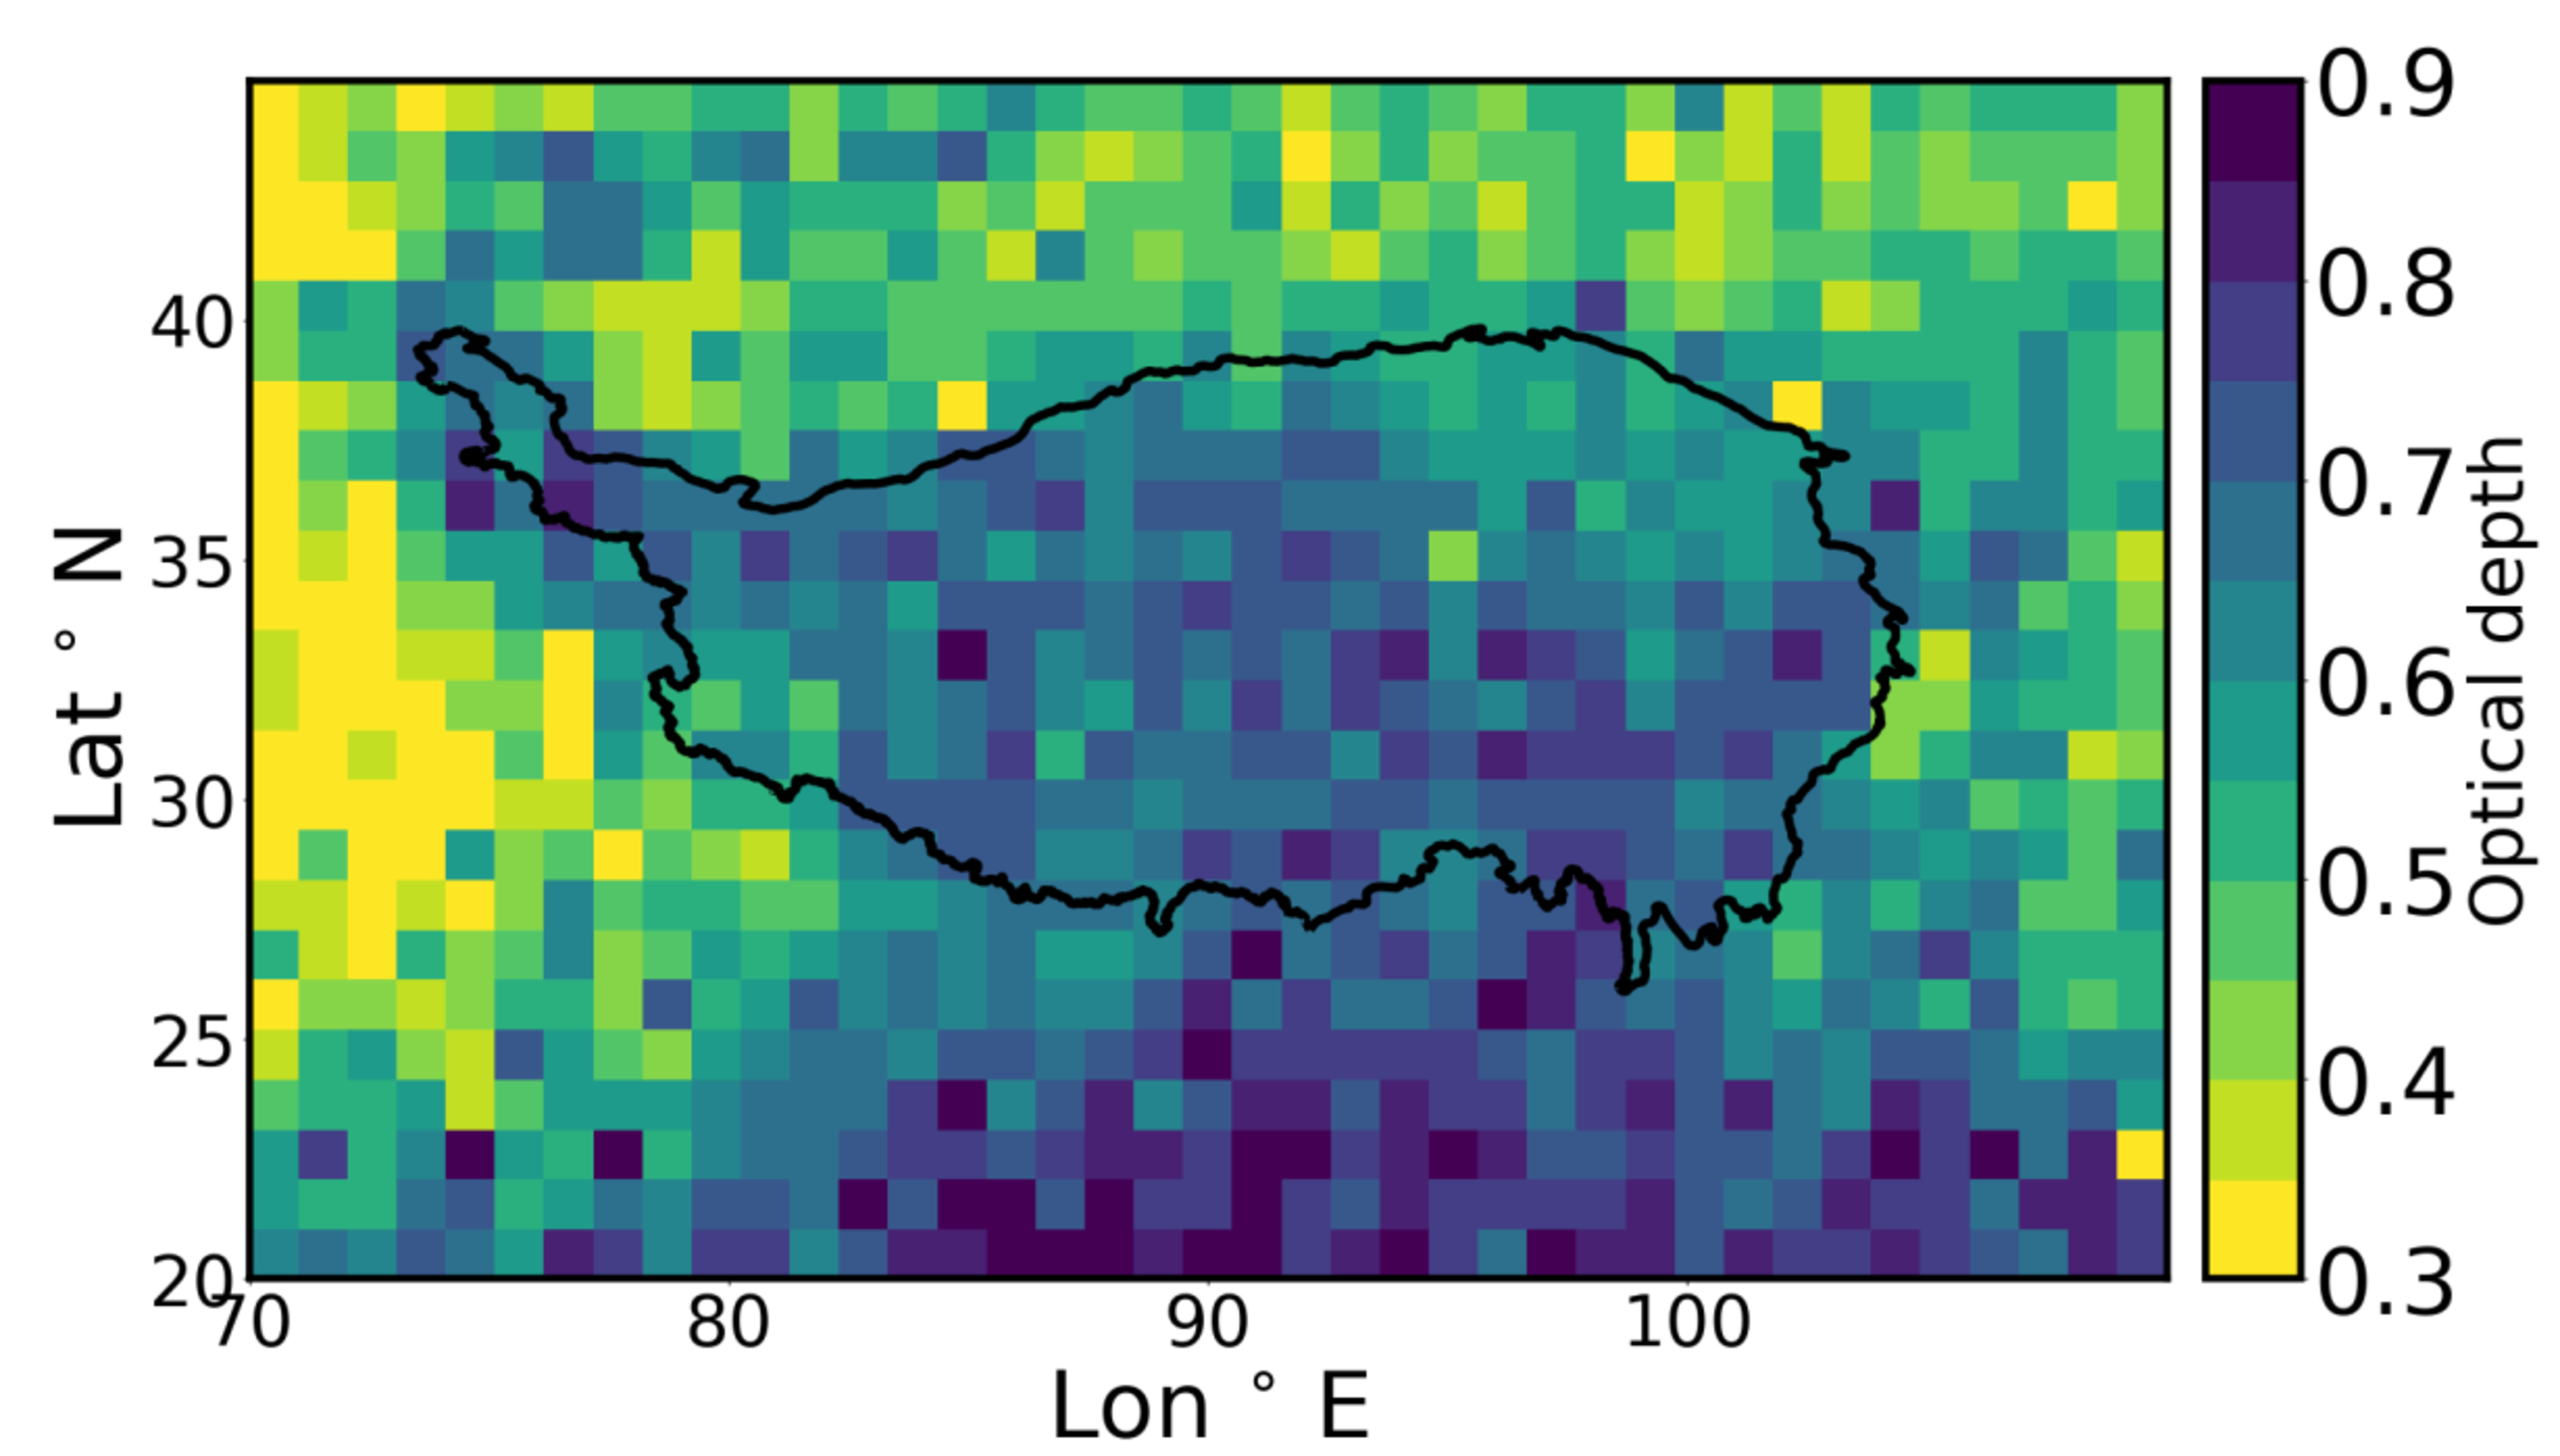
\includegraphics[width=\textwidth]{optical_depth_monsoonseason.png}
        \label{fig:od1}
    \end{subfigure}%
    \begin{subfigure}[b]{0.5\textwidth}
        \centering
        \caption{OD, Oct -- Apr} 
        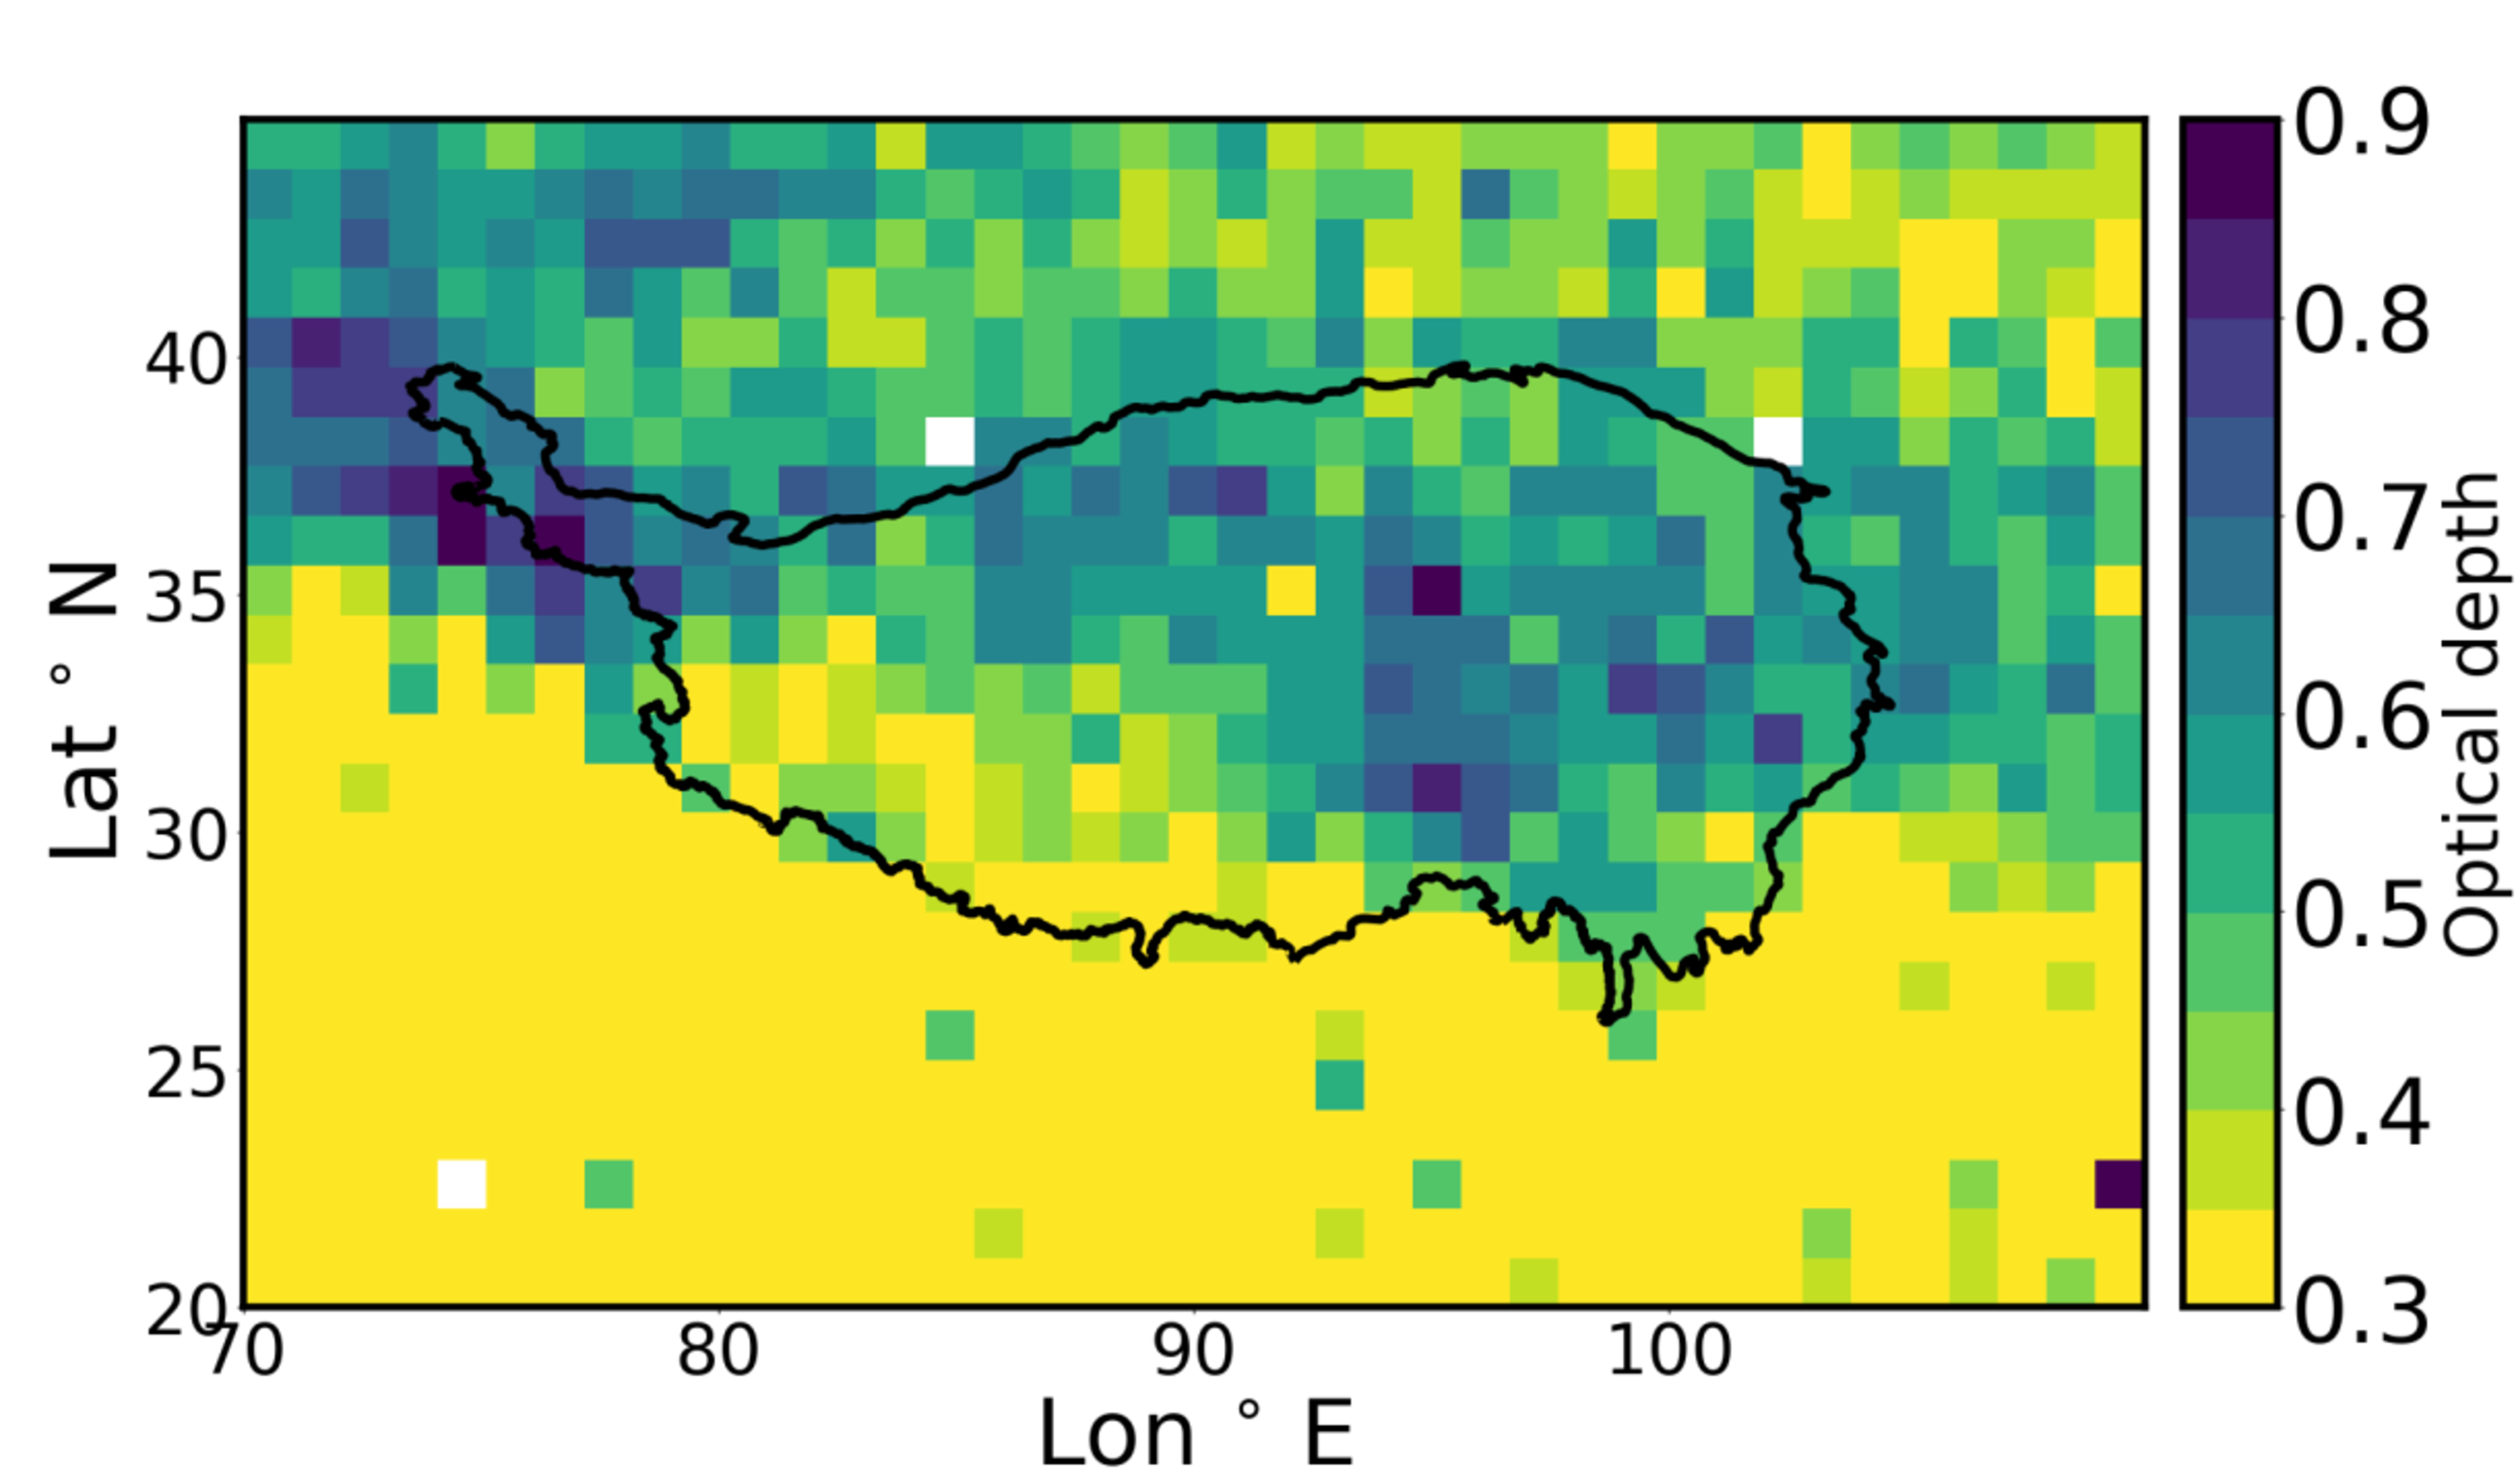
\includegraphics[width=\textwidth]{optical_depth_westerlyseason.png}
         \label{fig:od2}
    \end{subfigure}   
    
        \begin{subfigure}[b]{0.5\textwidth}
       \centering
        \caption{OD cloud layers, May -- Sep }       
        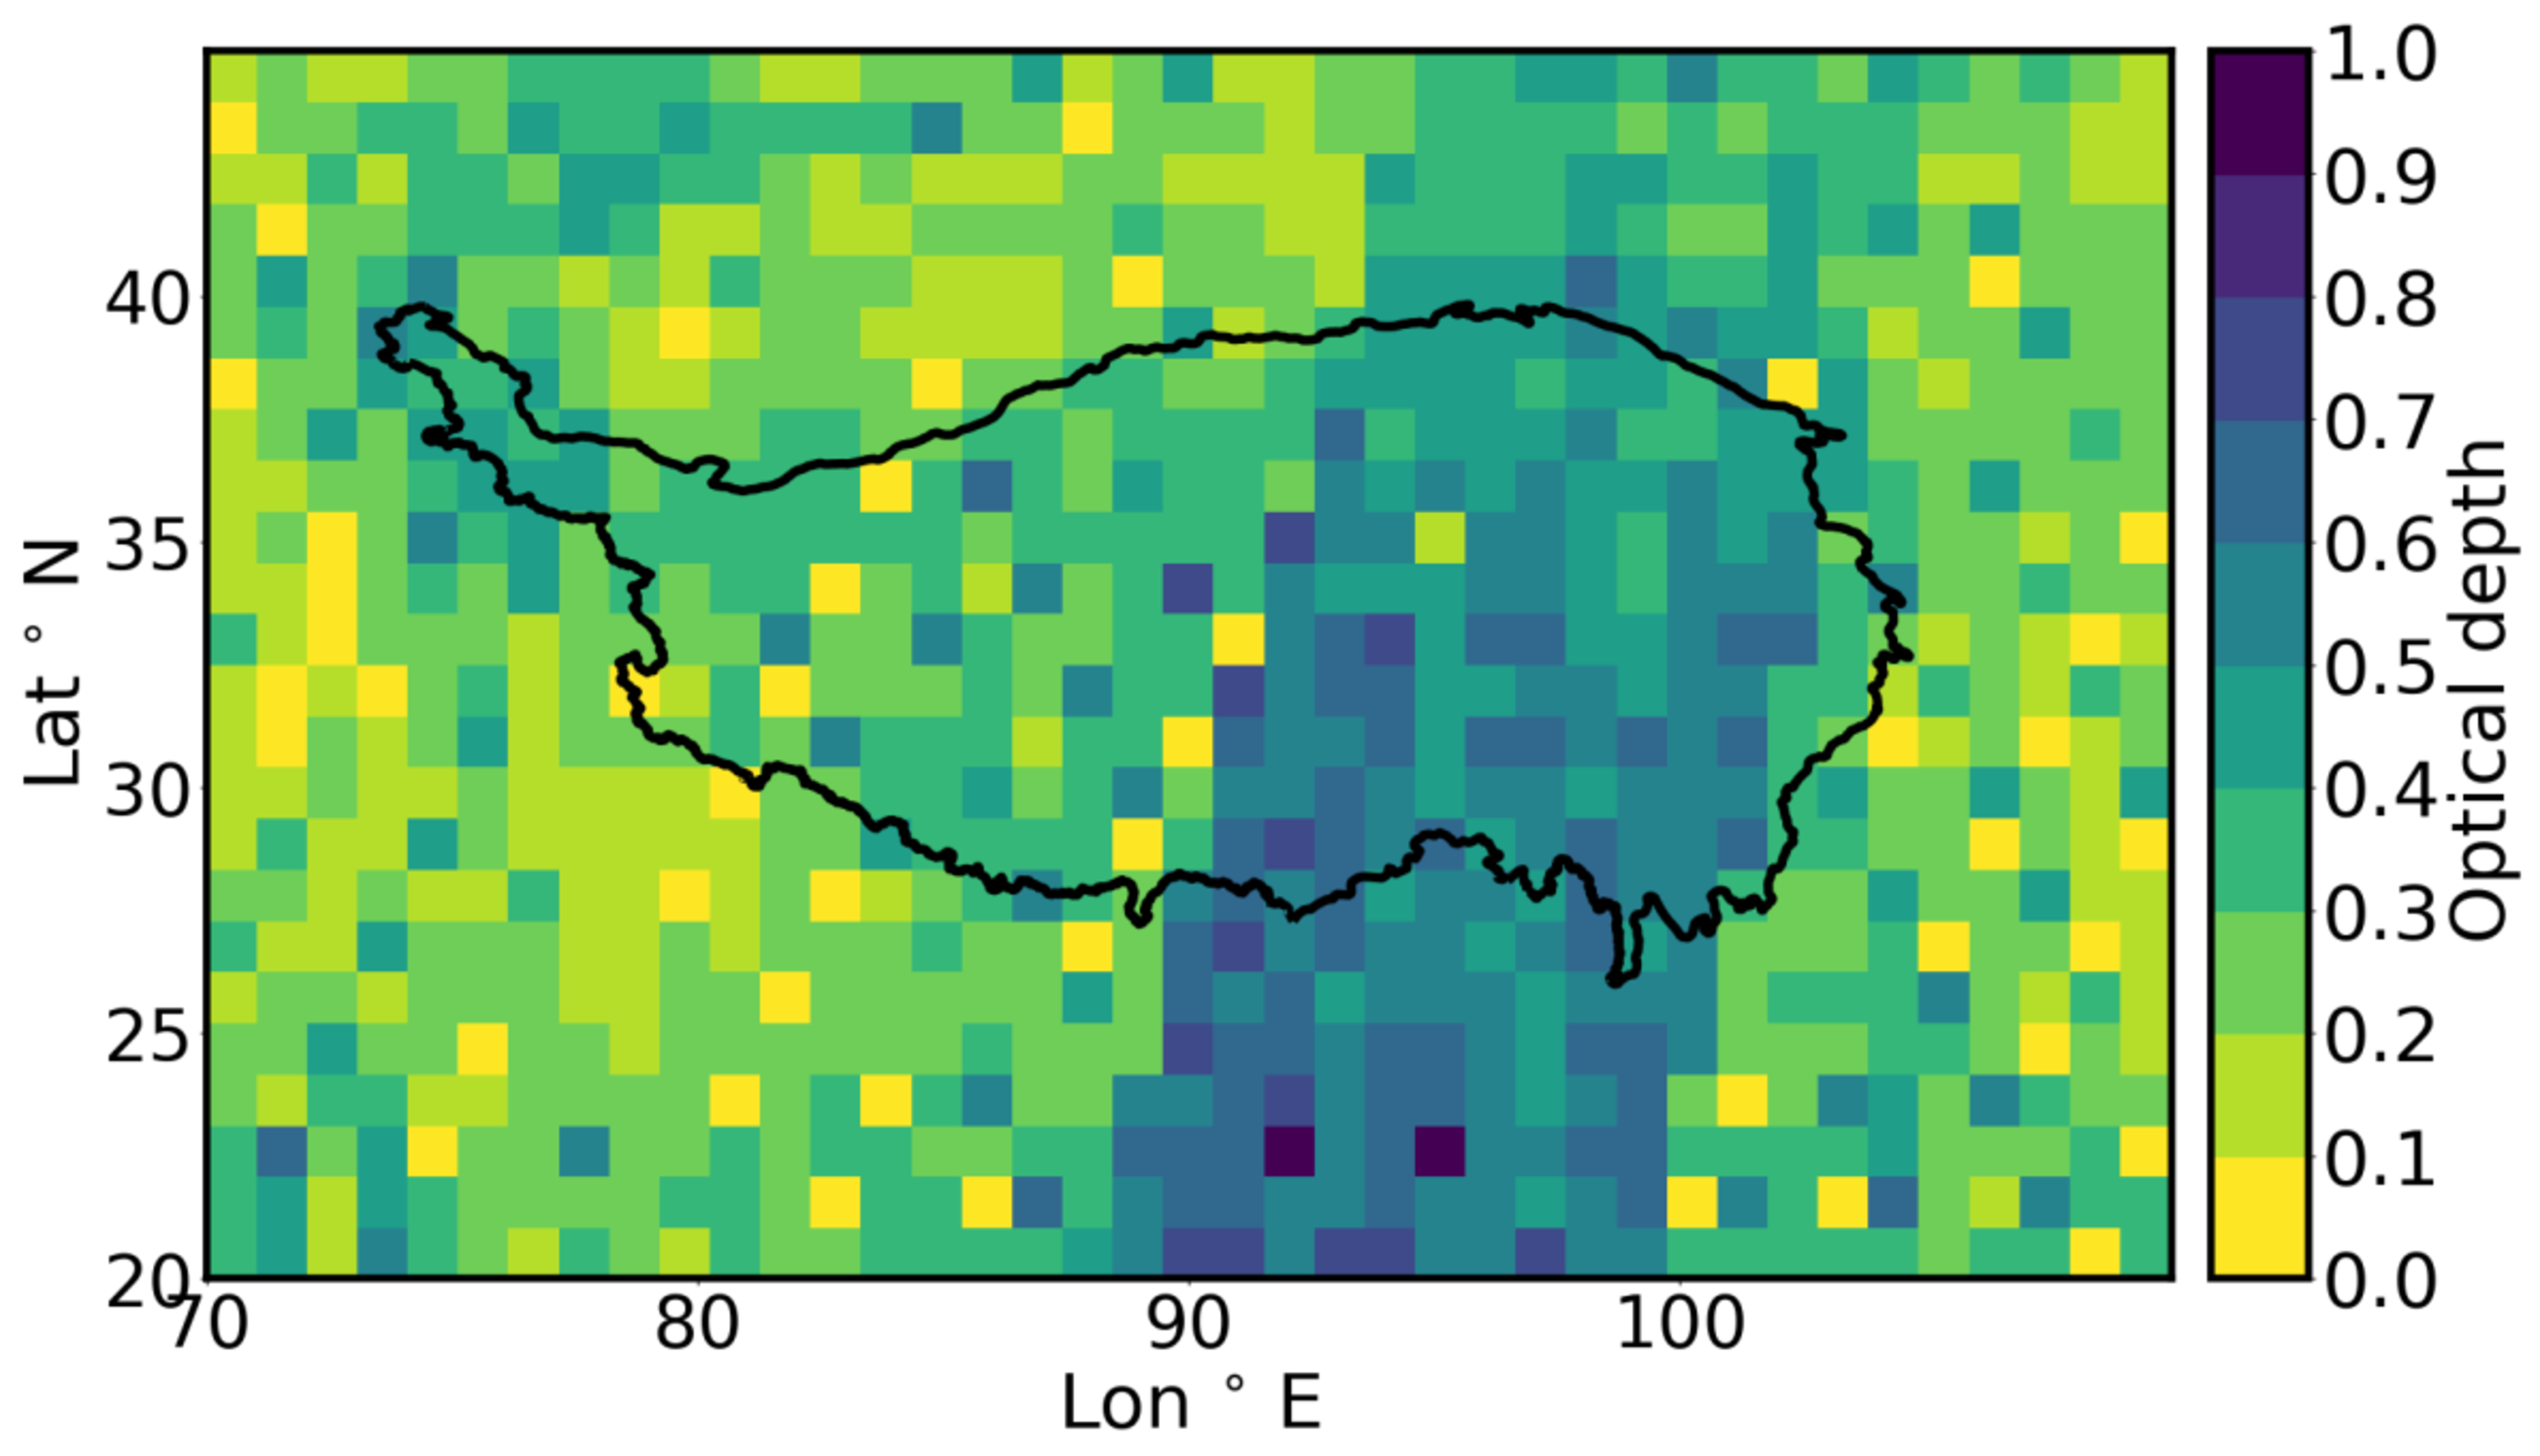
\includegraphics[width=\textwidth]{2C-ICE_OD_cld_occ_monsoon.png}
        \label{fig:od3}
    \end{subfigure}%
    \begin{subfigure}[b]{0.5\textwidth}
        \centering
        \caption{OD cloud layers, Oct -- Apr} 
        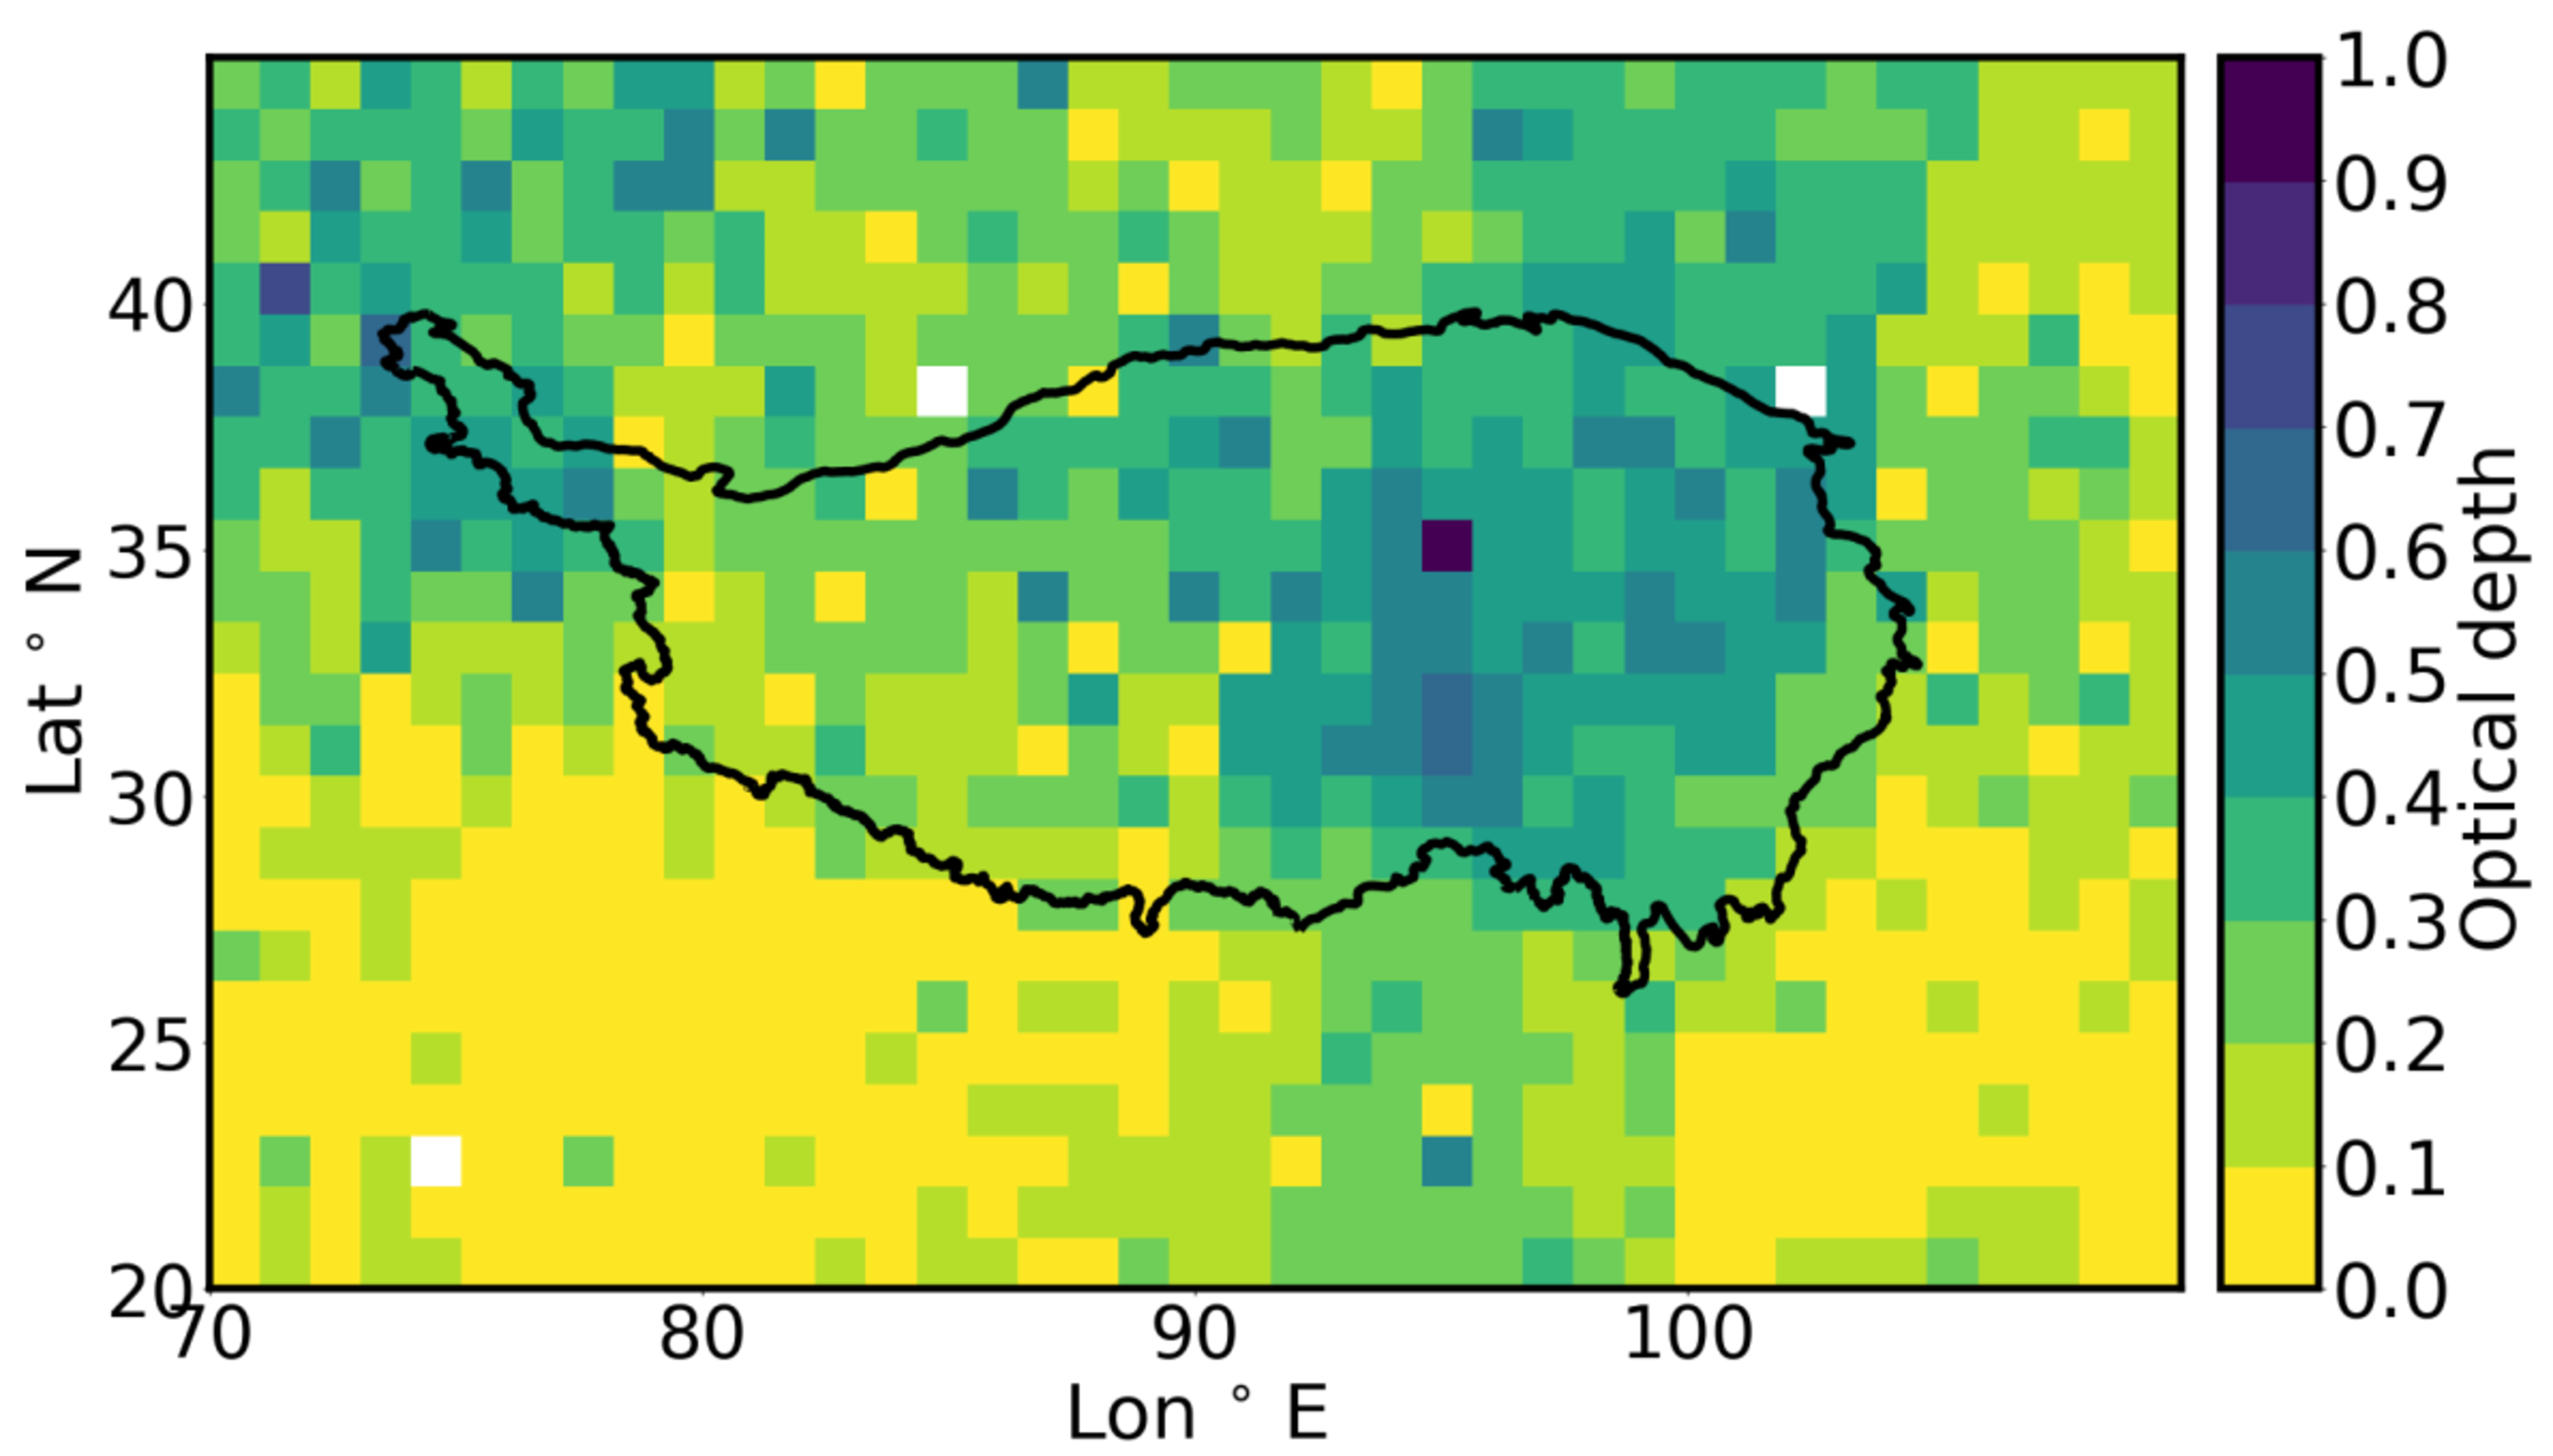
\includegraphics[width=\textwidth]{2C-ICE_OD_cld_occ_westerly.png}
         \label{fig:od4}
    \end{subfigure}   
    

    \begin{subfigure}[b]{0.5\textwidth}
       \centering
        \caption{liquid cloud layers, May -- Sep }       
        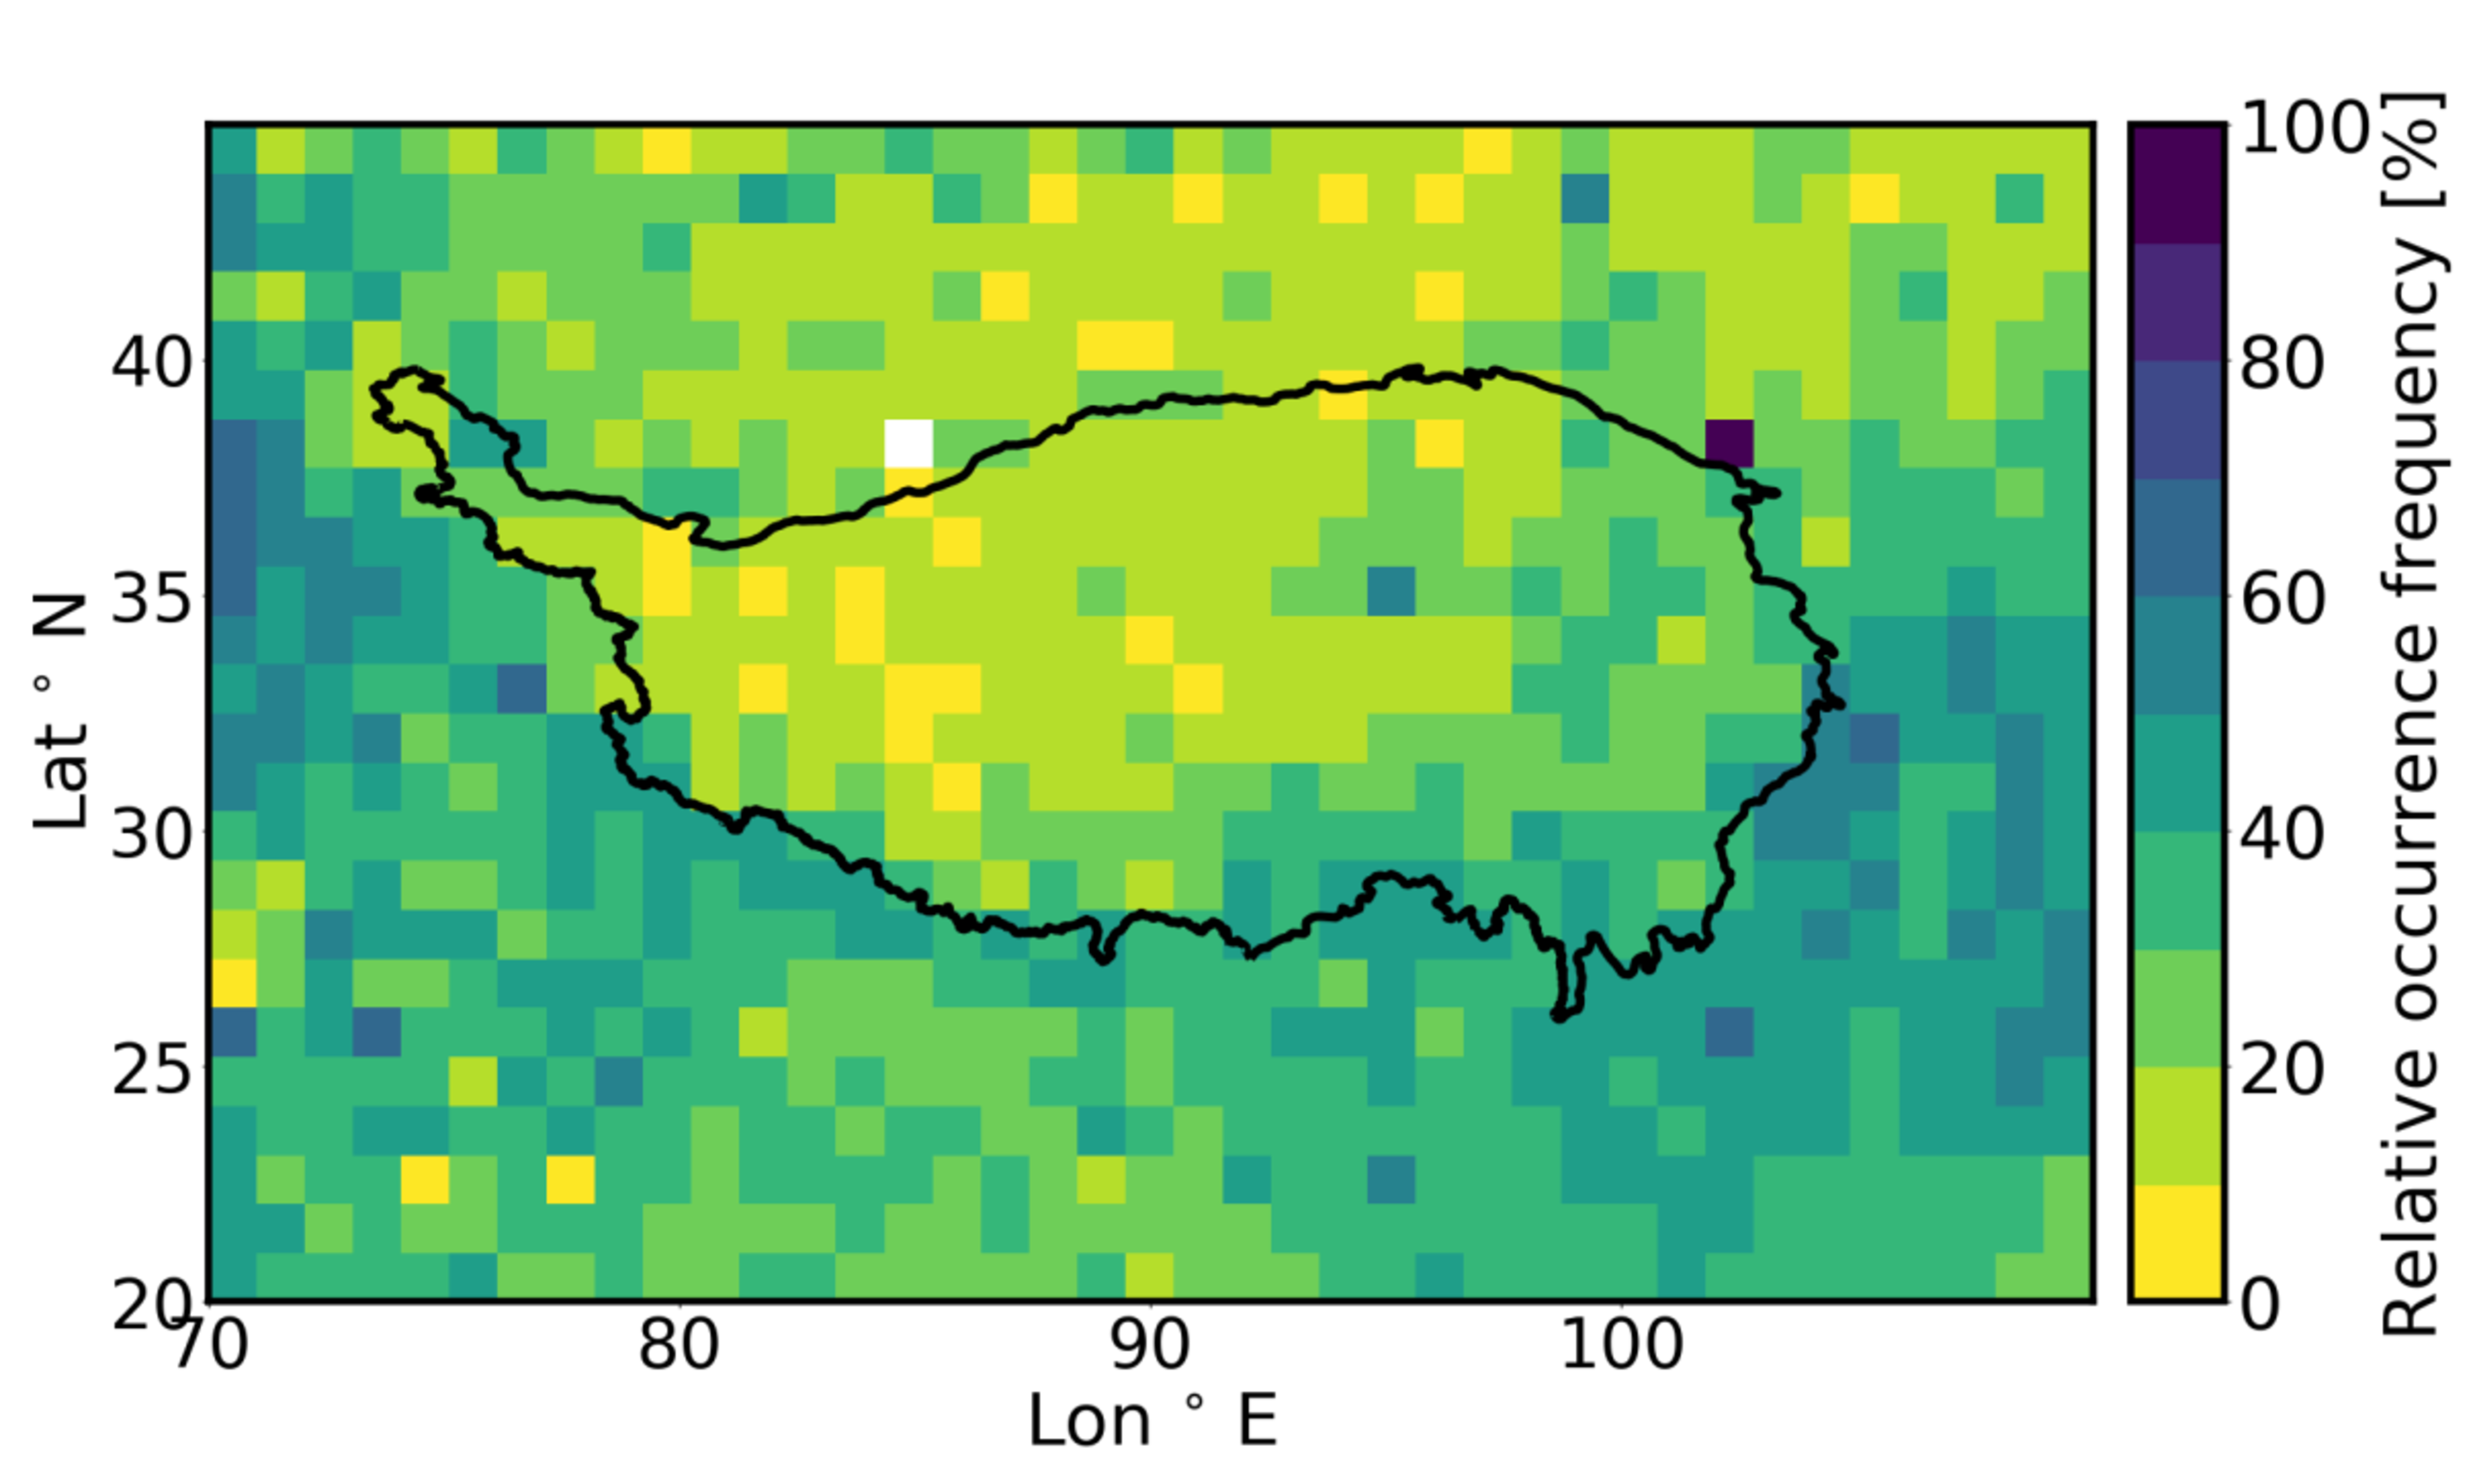
\includegraphics[width=\textwidth]{2B_CLDCLASS_liquid_monsoon.png}
        \label{fig:od5}
    \end{subfigure}%
    \begin{subfigure}[b]{0.5\textwidth}
        \centering
        \caption{liquid cloud layers, Oct -- Apr} 
        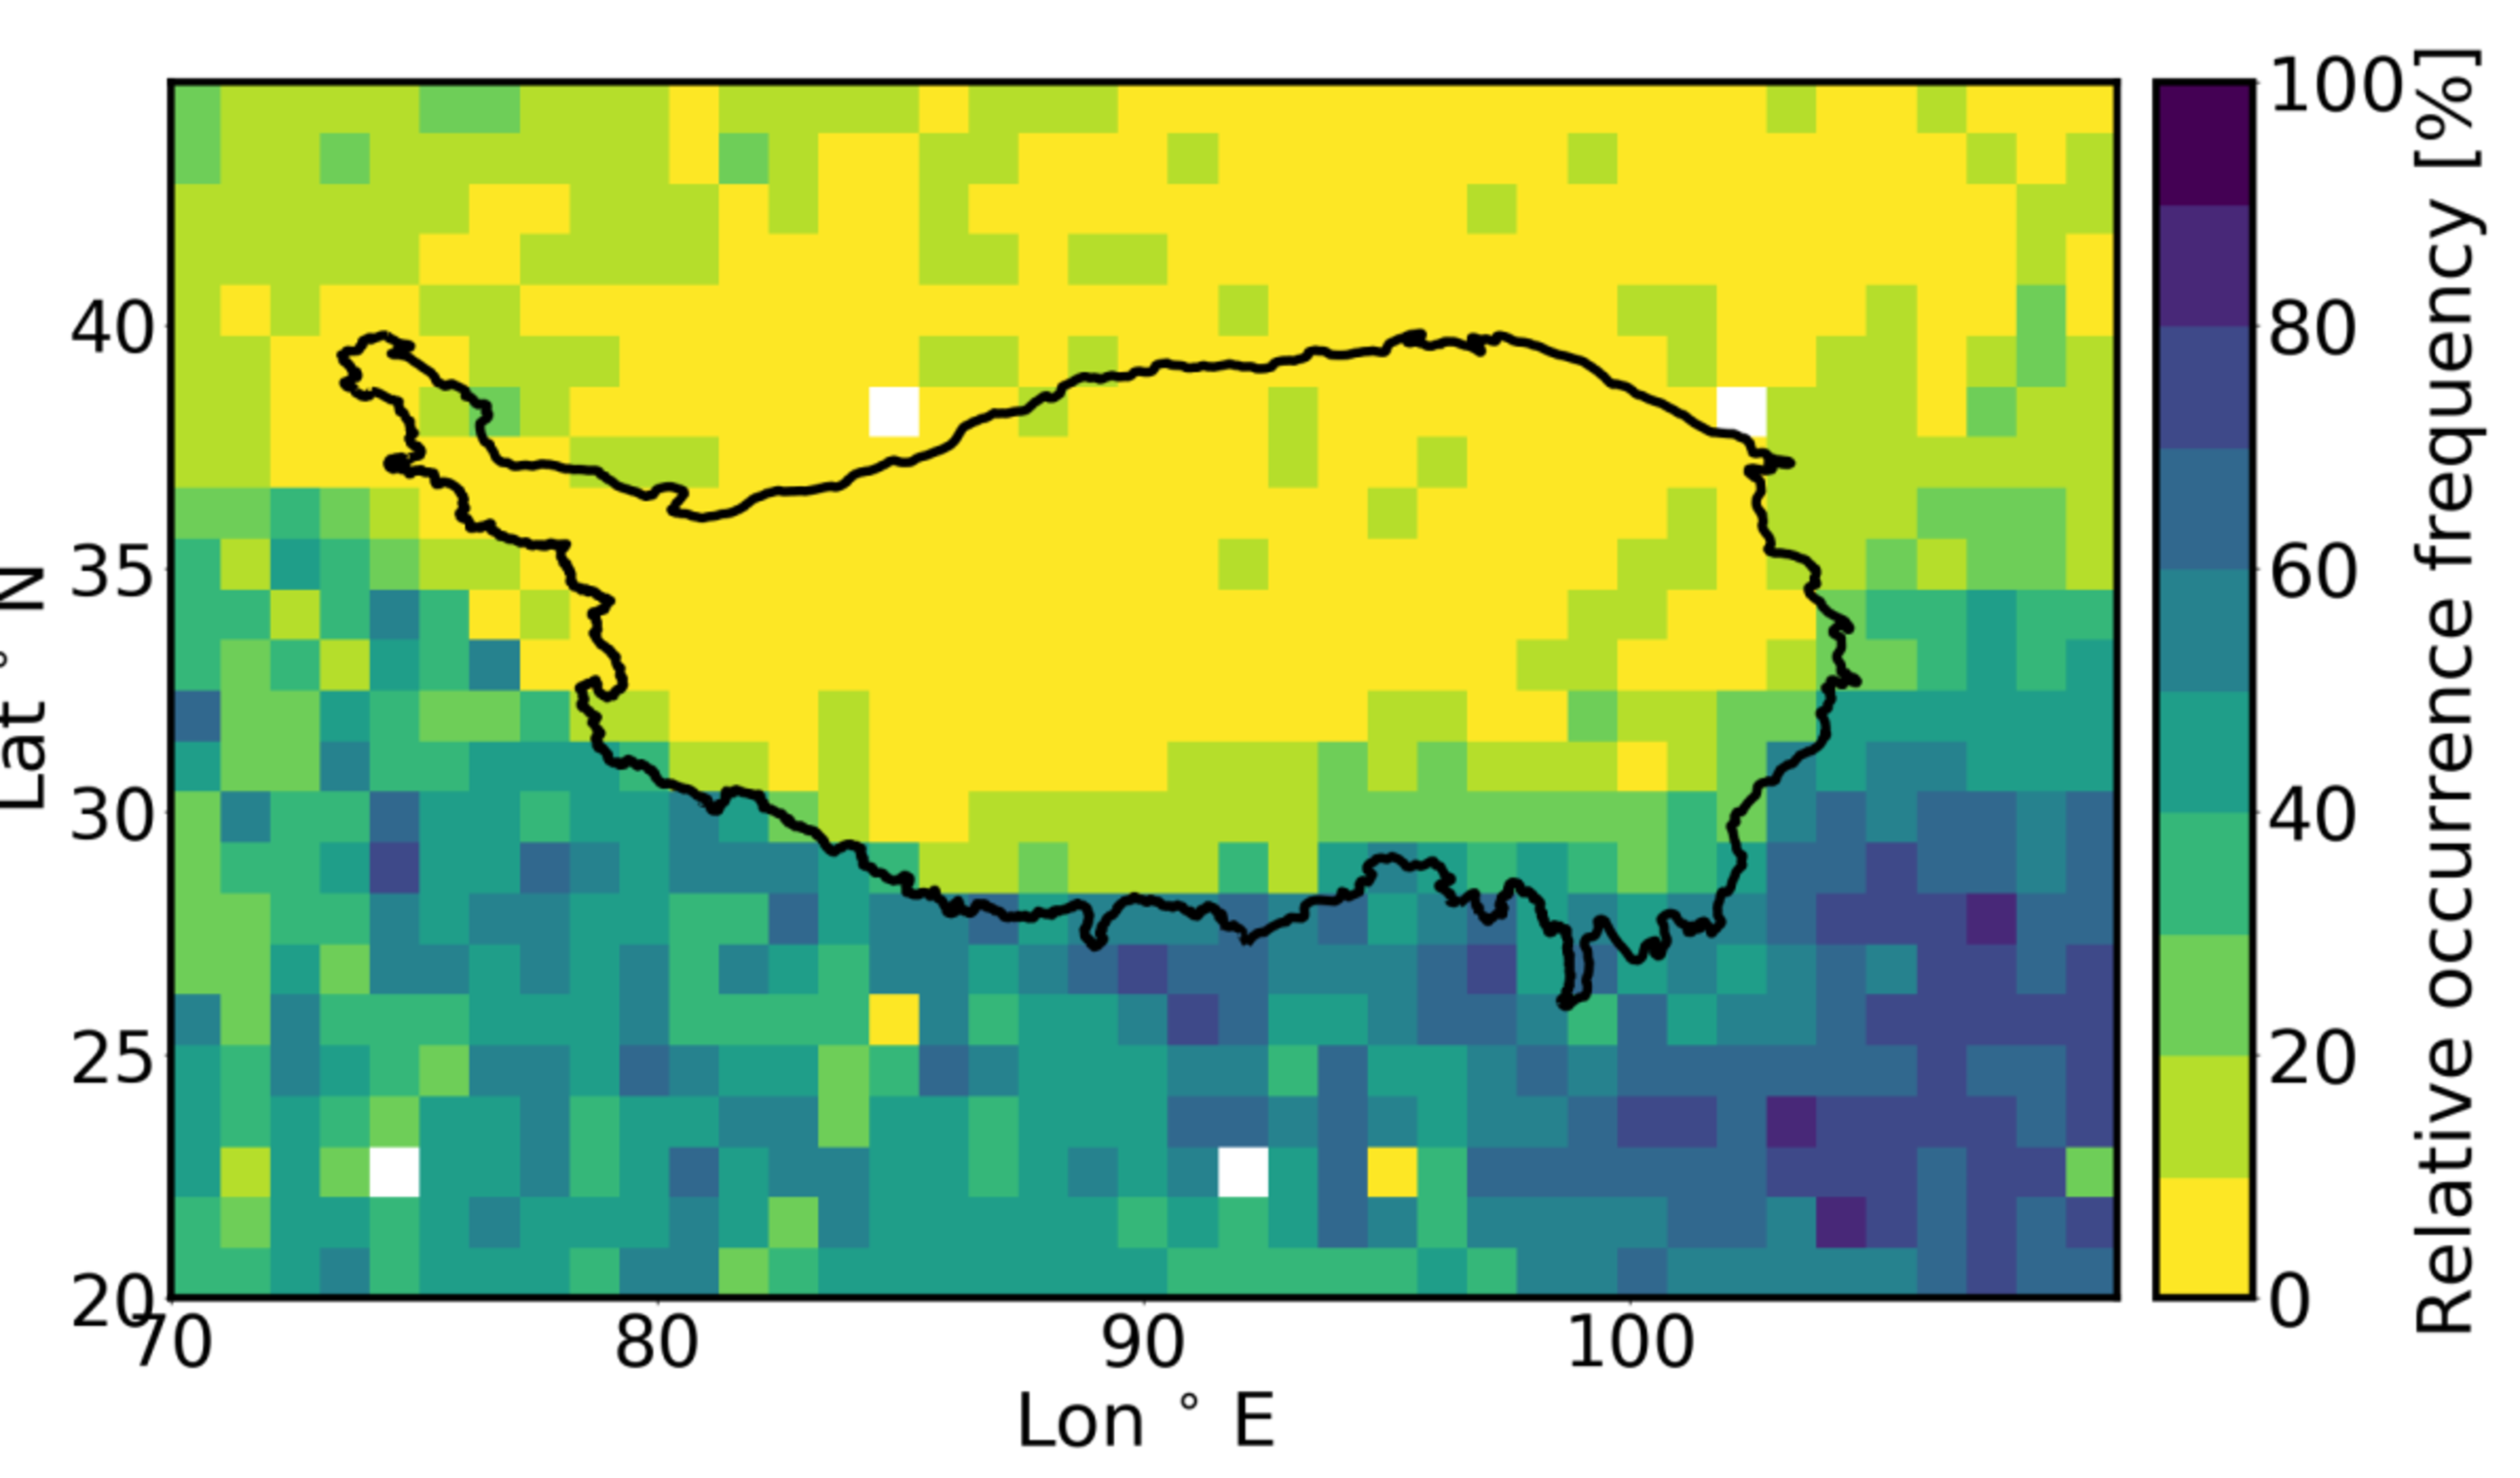
\includegraphics[width=\textwidth]{2B_CLDCLASS_liquid_westerly.png}
         \label{fig:od6}
    \end{subfigure}   
    
   
%\begin{figure}\ContinuedFloat
        \begin{subfigure}[b]{0.5\textwidth}
       \centering
        \caption{cloud layer base, May -- Sep }       
        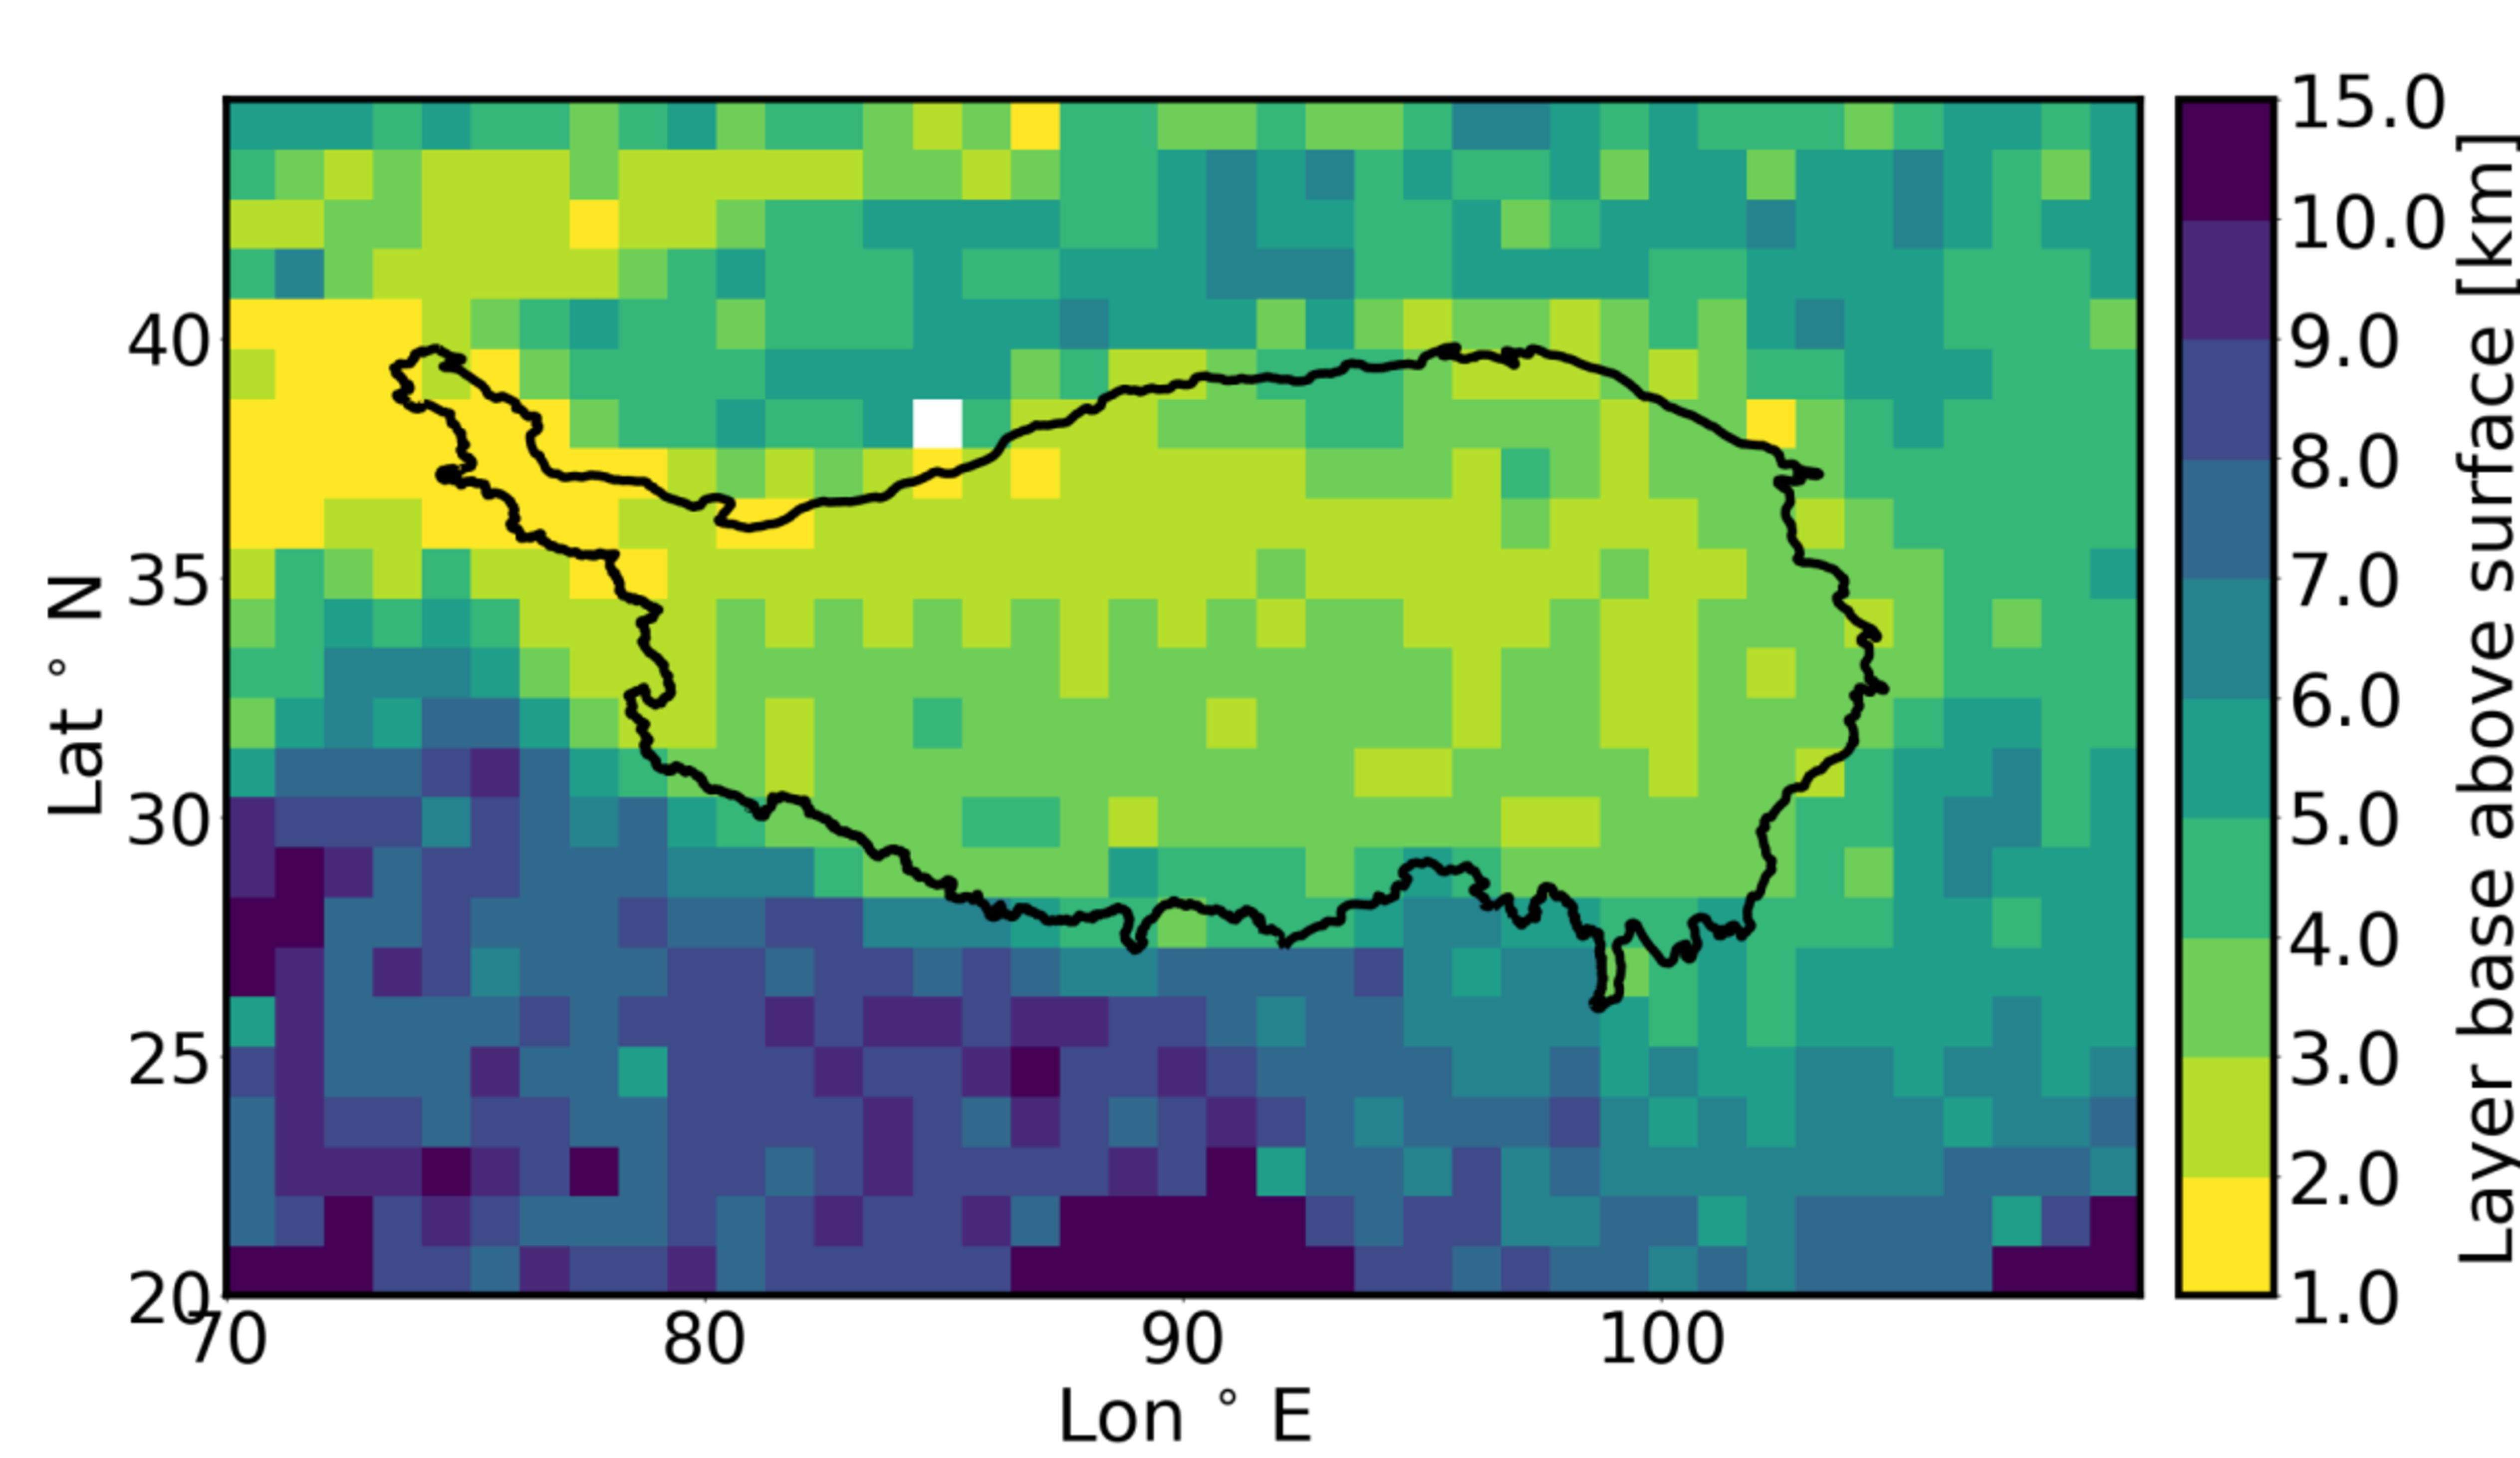
\includegraphics[width=\textwidth]{layerbase_median_monsoonseason.png}
        \label{fig:od7}
    \end{subfigure}%
    \begin{subfigure}[b]{0.5\textwidth}
        \centering
        \caption{cloud layer base, Oct -- Apr} 
        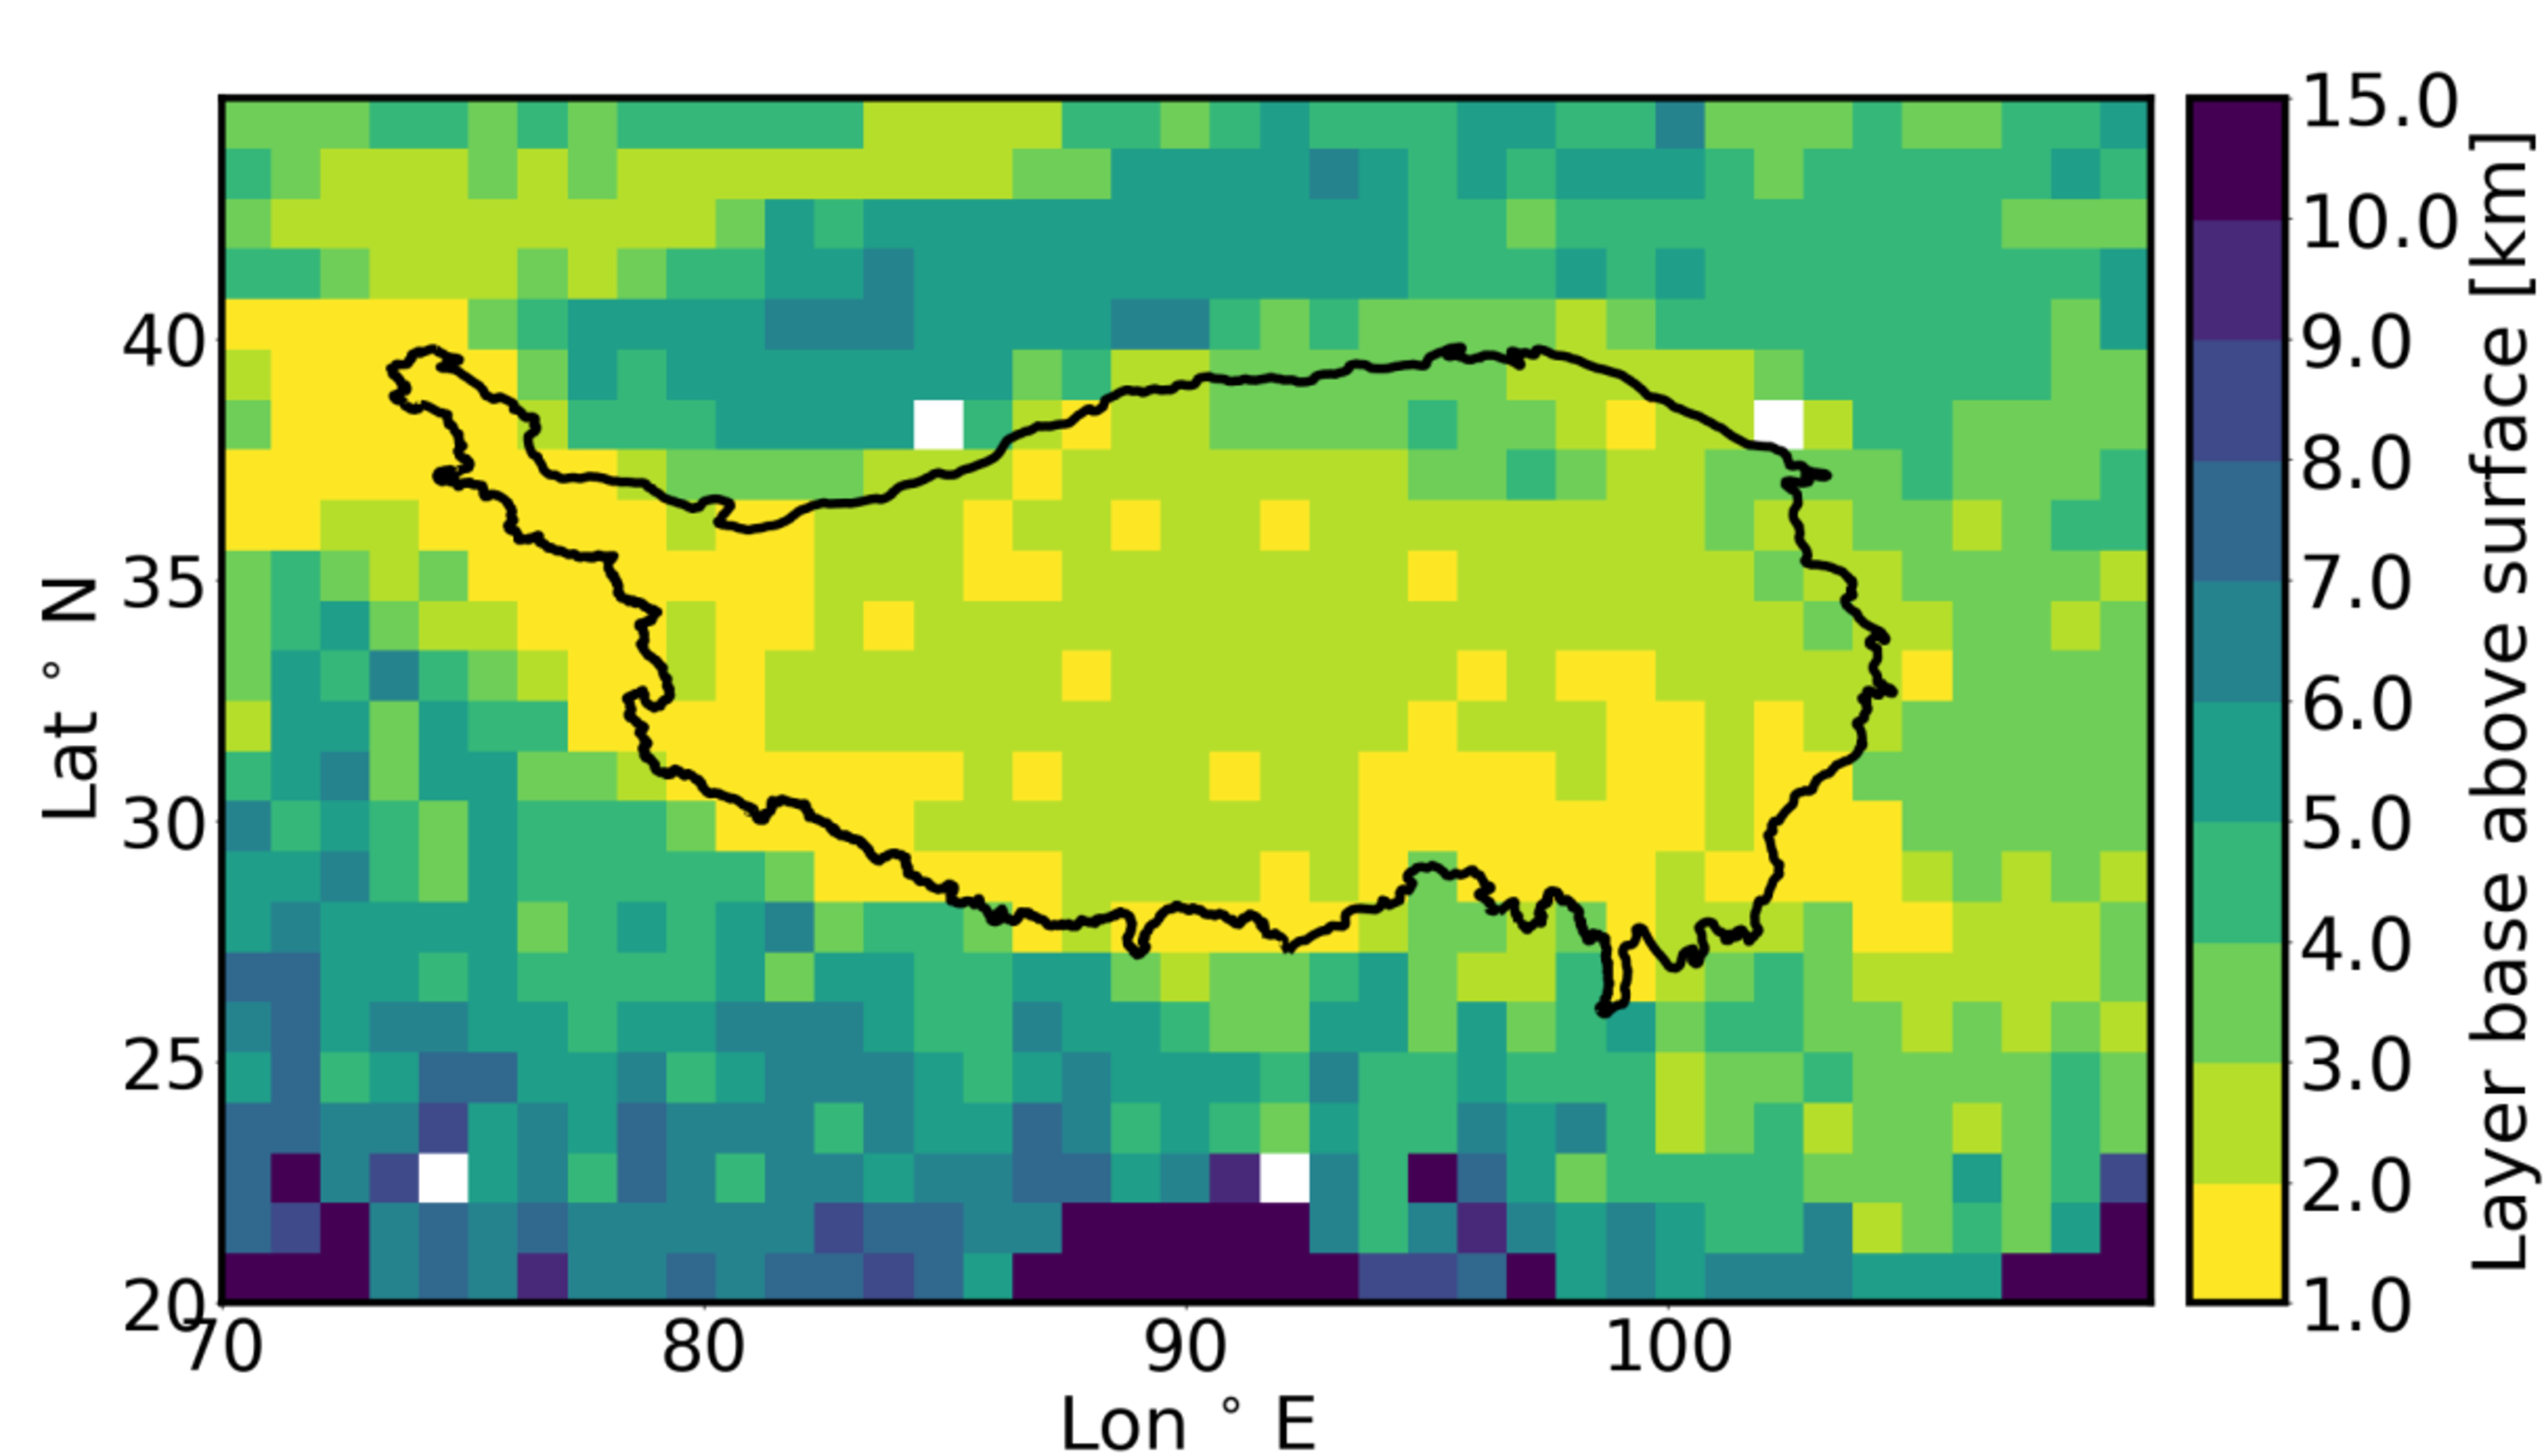
\includegraphics[width=\textwidth]{layerbase_median_westerlyseason.png}
       \label{fig:od8}
    \end{subfigure}   
    
    \caption{Optical depth (OD) and cloud properties over the TP for the monsoon season (May -- Sep) and (b) westerly season (Oct -- Apr) based on 2C-ICE (2007 – 2010).
    Figure (a) and (b) display the seasonal mean optical depth, (c) and (d) the seasonal optical depth values when at least one cloud layer is present, (e) and (f) the seasonal relative occurrence frequency of liquid cloud layers and (g) and (h) the seasonal median cloud layer base height for detected cloud layers.}
    \label{fig:od}
\end{figure}



\section{Conclusions and discussion}


In this study seasonal and diurnal variations of cloud occurrences, cloud types, cloud vertical structure and ice clouds have been investigated and compared between three subregions of the Tibetan Plateau. The results complement findings based on previous satellite observations and reveal significant differences in cloud characteristics between the examined seasons and regions. 
It was confirmed that low-level single-layer clouds generally dominate the TP during all seasons. Further, three key features of spatial and temporal variations in clouds over the TP have been established: 1) the significant contribution of stratiform and ice clouds, 2) the observed seasonality and 3) the observed regional differences according to the framework of \citet{cu13_2}. Since this study can serve as a pilot study to provide an overview of general variations in cloud properties, the elaborated key findings below can help to design future studies on convection processes and precipitation over the TP:


First, high occurrence frequencies of ice clouds and stratiform cloud types have been observed, especially in the westerly-dominated north and during the westerly season. This, for example, implies that a strengthening of westerlies in the future could lead to an enhanced effect of ice clouds on the thermal forcing. Further, the stratification of ice cloud layers can contribute to a possible mechanism for precipitation formation in addition to shallow convection, which could be important for the regional climate. We suggest therefore to further study the role of stratiform ice cloud layers for convection and precipitation.


Second, the monsoon season affects the TP in all three subregions and gives signals of increases in total cloud occurrences, liquid cloud layers and convective cloud types during the summer months. By taking advantage of the \textit{CloudSat-CALIPSO} daytime and nighttime overpasses, diurnal variations have been compared to the seasonal variations in this study. In general, the day-night differences are not as pronounced as variations between the westerly and monsoon season, even though hydrometeor and cloud layer occurrences during daytime are slightly higher than those during nighttime. 


Third, significant differences in cloud characteristics between the monsoon-dominated and westerly-dominated domains match with the differences associated with the respective seasons. During the monsoon season and in the monsoon-dominated south, higher variations in cloud types and cloud vertical structure could be observed due to the co-occurrence of high cirrus clouds and lower level cumulus. While both the monsoon season and the monsoon-dominated domain exhibit higher occurrence frequencies of low-level and convective cloud types with higher mean cloud thicknesses and optical depths, the dominating cloud type of in the westerly-dominated domain are ice clouds. This should be considered in future studies on changes in large-scale moisture transport and cloud feedbacks. Further, the cloud characteristics in the westerly-dominated domain appears to be closely linked with those in the transition zone, suggesting that the westerlies may have affected a larger region than assumed in the applied framework. 


An important implication of these three key findings is that changes in large-scale circulation might result in altered cloud patterns. Increases of snowfall in the northern TP due to a strengthening of westerlies, as suggested by \citet{c17}, could for example lead to an even stronger domination of ice clouds and hence an enhanced positive cloud radiative effect when these have high cloud top heights and low optical thicknesses.
Hence, future changes of westerlies and monsoon circulation might be crucial for cloud-radiation interactions, which at the current state are still dominated by a negative forcing/cooling effect \citep{cu16_2}. 
However, this study shows also that clouds over the TP are highly heterogenous. As a result, different regions might be unequally sensitive to changes of hydro-climatic regimes. \citet{karakoram2014snowfall} argue that precipitation over the Karakoram region is, for example, much less sensitive to the observed warming than the Himalayas, because it is dominated by the non-monsoonal moisture transport. For monsoon-associated convection, it remains unclear which of the two following processes dominates: shallow convection that prevents the formation of large-scale stratiform precipitation \citep{cu17_6} or the development of mesoscale convective systems during summertime \citep{cu08,cu16_4,cu17} resulting in higher occurrence frequencies of deep convection cells and cirrus clouds. Since the magnitude of elevation-dependent warming in the TP region in the future will also depend on cloud properties \citep{EDW2015}, the relative importance of stratification, mesoscale convective systems and advection for cloud formation need to be quantified. 


The nocturnal precipitation peaks over the TP which have been identified by several studies \citep[Kukulies et. al, \textit{unpublished manuscript}]{m10, m11, m11_2, m12_2} are not represented as larger cloud layer occurrences in the used data products, but as generally stronger \textit{CPR} signals. However, the fact that cloud layer occurrences are lower during night could be due to the coarse temporal resolution of \textit{CloudSat} and \textit{CALIPSO}. 



It should also be noted that the used datasets are global data products, so general retrieval assumptions might deviate from the climate conditions of the TP. In order to validate the importance of ice clouds in the TP region, the 2C-ICE product needs therefore to be calibrated with data from geostationary satellites. Furthermore, we suggest that the boundary of the westerly-dominated zone of the TP can be more south, because the transition zone showed more similar cloud properties to the westerly-dominated domain. The gridded data also revealed significant east-west differences in cloud properties, so this study together with Part 2 of this paper (\textit{and other research?}) could be used to determine new borders for regions of large-scale impact \citep{cu13_2}. 


Finally, the regional and seasonal division in this paper focuses on linkages between cloud formation and the large-scale circulation. However, other factors such as aerosol forcing and local surface heating control convection. \citet{d2007summer} found that a significant portion of dust aerosols from the Taklimakan Desert affects the TP during the summer months. The reason for the increase in cloud occurrences during summer in the westerly-dominated domain and transition zone may not only indicate the transport of moisture and cloud systems by the monsoon circulation, but could also be attributed to higher surface temperatures as a control for local convection and a higher availability of CCN and IN from dust aerosols. 


\clearpage

%%%%%%%%%%%%%%%%%%%%%%%%%%%%%%%%%%%%%%%%%%%%%%%%%%% tables %%%%%%%%%%%%%%%%%%%%%%%%%%%%%%%%%%%%%%%%%%%%%%%%%%

\begin{table}[h!]
\centering
\scriptsize
\caption{Overview of combined \textit{CloudSat-CALIPSO} data products used in this study.}
\begin{threeparttable}
\begin{tabular}{lccrrr}
\headrow
\thead{Satellite} & \thead{Data product} & \thead{Parameters} & \thead{Sensor} & \thead{Resolution} & \thead{Period}\\
\textit{CloudSat} & \textbf{2B-GEOPROF}&  CPR mask, radar reflectivity & CPR & 0.24 km vertical, 1.3 x 1.7 km horizontal &2006 -- 2011 \\
\textit{CloudSat, CALIPSO } & \textbf{2B-GEOPROF-LIDAR } & lidar cloud fraction, layer amount & CPR, CALIOP  &0.24km vertical, 1.3 x 1.7 km horizontal & 2006 -- 2011 \\
\textit{CloudSat, CALIPSO } & \textbf{2B-CLDCLASS-LIDAR }& layer type, particle phase, layer base and top height  & CPR, CALIOP& 5 layers vertical, 1.3 x 1.7 km horizontal &2007--2010 \\
\textit{CloudSat, CALIPSO } & \textbf{2C-ICE} &  column-integrated optical depth &   CPR, CALIOP  &0.24km vertical, 1.3 x 1.7 km horizontal  & 2007--2010\\
\hline  % Please only put a hline at the end of the table
\end{tabular}
\end{threeparttable}
\label{tab:data}
\end{table}




\begin{table}[h!]
\centering
\caption{Number of profiles in  2B-GEOPROF/2B-GEOPROF-LIDAR (2006 -- 2011).}
\scriptsize\begin{tabular}{l l l l}
\hline
domain & day overpass& night overpass & total \\
monsoon-dominated&  254 354              & 252 347         &  506 701 \\
transition zone & 825 414 &   824 772    & 1 650 186 \\
westerly-dominated &   595 436   &  598 725   &1 194 161 \\
total & 1 675 204 &  1 675 844 & 3 351 048  \\
\end{tabular}
\label{tab:profilenr}
\end{table}


\begin{table}[!h]
\centering
\caption{Contribution of profile samples (\%) from 2B-GEOPROF/2B-GEOPROF-LIDAR (2006 -- 2011) which were found to be cloudy, separated into profiles which contain hydrometeors and profiles with at least one continuous cloud layer. All cloud occurrences are displayed for different subregions and separated into day and nighttime.}
\label{tab:profile_stats}
\noindent{\small\begin{tabular}{l l l l l l l}
domain & hydrometeors & cloud layer &  hydrometeors&  cloud layer & hydrometeors & cloud layer \\
& daytime  & daytime  & nighttime  & nighttime  & total  &  total  \\
monsoon-dominated&  76& 75 &  70& 67 & 73& 71  \\
transition zone & 75& 74  &   66& 64 & 70& 69  \\
westerly-dominated &  73& 72   &  71& 68    & 72& 70 \\
total &  75& 74   &  68& 66   & 72& 70  \\        
\end{tabular}}
\end{table}





\clearpage

%-------------------------------------end of article------------------------------------------------------------------
\section*{acknowledgements}
This research was part of the Swedish National strategic research programs BECC and MERGE.

\section*{conflict of interest}
%You may be asked to provide a conflict of interest statement during the submission process. Please check the journal's author guidelines for details on what to include in this section. Please ensure you liaise with all co-authors to confirm agreement with the final statement.
No competing interests. 

%\printendnotes

% Submissions are not required to reflect the precise reference formatting of the journal (use of italics, bold etc.), however it is important that all key elements of each reference are included.


% USING BIBTEX: 
\bibliographystyle{apa}  % choose reference style 
\bibliography{references.bib}


\end{document}
